\documentclass[12pt,usenames,dvipsnames]{beamer}
\mode<presentation>
{
  \usetheme{default}      % or try Darmstadt, Madrid, Warsaw, ...
  \usecolortheme{default} % or try albatross, beaver, crane, ...
  \usefonttheme{serif}  % or try serif, structurebold, ...
  \setbeamertemplate{navigation symbols}{}
  \addtobeamertemplate{navigation symbols}{}{%
  	\usebeamerfont{footline}%
    \usebeamercolor[fg]{footline}%
    \hspace{1em}%
    \insertframenumber
  } 
  \setbeamertemplate{caption}[numbered]
}

\usepackage{newpxtext}
\usepackage{newpxmath}

\usepackage[english]{babel}
\usepackage[utf8x]{inputenc}
\usepackage{changepage}
\usepackage{filecontents}
\usepackage{lipsum}
\usepackage{pgfplots}
\usepackage{physics}
\usepackage{siunitx}

\pgfplotsset{compat=1.14}

\usetikzlibrary{external}
\tikzexternalize

\newcommand\pro{\item[$\textcolor{ForestGreen}{+}$]}
\newcommand\con{\item[$\textcolor{BrickRed}{-}$]}
\definecolor{IMS}{RGB}{41, 120, 138}

\setbeamercolor{title}{fg=IMS!70!black}
\setbeamercolor{frametitle}{fg=IMS!70!black}
\setbeamercolor{itemize item}{fg=IMS!70!black}

\title{{\small\textsc{Tu1E}}\\A self-consistent integral equation framework for simulating optically-active media}
\author[shortname]{Connor Glosser\inst{1,2} \and B.\ Shanker \inst{2} \and \mbox{Carlo Piermarocchi\inst{1}}}
\institute[MSU]{
  \inst{1} Michigan State University, Dept.\ of Physics \& Astronomy \and %
    \inst{2} Michigan State University, Dept.\ of Electrical \& Computer Engineering
}

\date{\today}

\setbeamertemplate{background}{
  \includegraphics[width=\paperwidth,height=\paperheight,keepaspectratio]{figures/background}
}

\begin{document}

\begin{frame}
  \titlepage
\end{frame}

\begin{frame}{We study quantum dots because \\ of their technological applications}
  \vspace{-1cm}
  \begin{columns}
    \begin{column}{0.25\textwidth}
      \begin{center}
        Photovoltaics
      \end{center}
    \end{column}

    \begin{column}{0.25\textwidth}
      \begin{center}
        Next-gen displays
      \end{center}
    \end{column}

    \begin{column}{0.25\textwidth}
      \begin{center}
        Biological contrast
      \end{center}
    \end{column}

    \begin{column}{0.25\textwidth}
      \begin{center}
        Quantum computing
      \end{center}
    \end{column}

  \end{columns}

  \begin{columns}
    \begin{column}{0.25\textwidth}
      \begin{figure}
        \includegraphics[width=\textwidth]{figures/devices/quantum_dot_solar_cell.jpg}
      \end{figure}
    \end{column}

    \begin{column}{0.25\textwidth}
      \begin{figure}
        \includegraphics[width=\textwidth]{figures/devices/quantum_dot_tv.jpg}
      \end{figure}
    \end{column}

    \begin{column}{0.25\textwidth}
      \begin{figure}
        \vspace{-1.2em}
        \includegraphics[width=\textwidth, height=0.4\textheight]{figures/devices/contrast.jpg}
      \end{figure}
    \end{column}

    \begin{column}{0.25\textwidth}
      \begin{figure}
        \includegraphics[width=\textwidth]{figures/devices/quantum_computer.jpg}
      \end{figure}
    \end{column}
  \end{columns}
\end{frame}

\begin{frame}{We need a fast, high-resolution model}
  \vspace{-0.2cm}
  \begin{columns}[t]
    \begin{column}{0.33\textwidth}
      \centering
      Macroscopic coupled PDEs
      \begin{itemize}
        \pro Easy
        \pro Fast
        \con Low resolution
        \con No mechanism for disorder
      \end{itemize}
      ``Maxwell-Bloch''
    \end{column}
    \vrule
    \begin{column}{0.33\textwidth}
      \centering
      Mesh-based models
      \begin{itemize}
        \pro Higher resolution
        \con Expensive
        \con Long-range sensitivities
        \con Short-range sensitivities
      \end{itemize}
      FEM/FDTD
    \end{column}
    \vrule
    \begin{column}{0.33\textwidth}
      \centering
      \emph{Ab initio} quantum simulation
      \begin{itemize}
        \pro Highest resolution
        \pro No quantum approximations
        \con Statistical or \emph{crazy} expensive
      \end{itemize}
      DFT, Quantum Monte Carlo
    \end{column}
  \end{columns}
  \begin{center}
    \textcolor{BrickRed}{We're interested in devices with randomness; \\ so-called ``random lasers''} 
  \end{center}
\end{frame}

\begin{frame}{The Liouville equation governs \\ internal QD dynamics}
  \begin{columns}
    \begin{column}{0.5\textwidth}
      \begin{equation*}
          \pdv{\hat{\rho}}{t} = \frac{-i}{\hbar} \commutator{\hat{\mathcal{H}}(t)}{\hat{\rho}} - \hat{\mathcal{D}}\qty[\hat{\rho}]
        \end{equation*}
        \begin{itemize}
          \item Mixed-state analogue of the Schr\"odinger equation
          \item Incorporate emission effects through $\hat{\mathcal{D}}[\hat{\rho}]$
          \item Rabi cycle; nonlinear system
        \end{itemize}
    \end{column}
    \begin{column}{0.5\textwidth}  %%<--- here
      \includegraphics[width=0.95\textwidth]{figures/rabi_oscillations}
      \begin{align*}
          \hat{\mathcal{H}}(t) &\equiv \mqty(0 & \vb{d} \cdot \vb{E}(t) \\ \vb{d}^* \cdot \vb{E}^*(t) & \hbar \omega_0) \\
            \hat{\mathcal{D}}[\hat{\rho}] &\equiv \mqty( (\rho_{00} - 1)/T_1 & \rho_{01}/T_2 \\ \rho_{10}/T_2 & \rho_{11}/T_1)
        \end{align*}
    \end{column}
  \end{columns}
\end{frame}

\begin{frame}{A rotating-frame transformation \\ affords \emph{much} larger timesteps}
  \begin{equation*}
    \dv{\tilde{\rho}}{t} = \frac{-i}{\hbar} \commutator{\hat{U} \hat{\mathcal{H}} \hat{U}^\dagger - i \hbar \hat{V}}{\tilde{\rho}} - \hat{\mathcal{D}}\qty[\tilde{\rho}], \quad \hat{V} \equiv \hat{U} \dv{\hat{U}^\dagger}{t}
  \end{equation*}
  \begin{columns}
    \begin{column}{0.4\textwidth}
      \begin{equation*}
        \hat{U} = \mathrm{diag}(1, e^{i \omega_L t})
      \end{equation*}
      \vspace{-0.5cm}
      \begin{alertblock}{Problem}
        Larger $\Delta t$ means larger ``spheres of influence.'' How do we maintain phase information?
      \end{alertblock}
    \end{column}
    \begin{column}{0.6\textwidth}
      \begin{filecontents}{fourier_pseudospin_zoom.dat}
2.5007077522574755  -80.28204547494957  -59.32281412952867  -59.40014806421626  -58.69284778426713
2.503849344911065 -80.19542002393177  -59.05702547174588  -59.426189934574765 -58.7023401775675
2.506990937564655 -80.10815921351903  -58.91100901450181  -59.174865815543704 -58.7118322308395
2.5101325302182445  -80.02025473662691  -59.040195629110485 -59.184786381668  -58.721292475496895
2.5132741228718346  -79.9316984431648 -58.696611083659405 -59.01655046723582  -58.730753442421644
2.5164157155254243  -79.84248205589894  -58.79382206181233  -58.929511817086215 -58.740184352810054
2.519557308179014 -79.75259673225341  -58.50127709905604  -58.744064527497144 -58.74961471366203
2.522698900832604 -79.66203380727421  -58.51521996026008  -58.75743213753444  -58.7590126700285
2.5258404934861937  -79.57078461392274  -58.2893366409114 -58.612636931589044 -58.768414409996
2.5289820861397834  -79.47883939705187  -58.34938071118141  -58.40672329873932  -58.777782555285555
2.532123678793373 -79.38618921217038  -58.203721749747004 -58.37781198922408  -58.78715129054602
2.535265271446963 -79.29282610070105  -57.97940703443358  -58.451256161961695 -58.796492950571384
2.538406864100553 -79.19873615979719  -58.04225577536915  -58.026383883109744 -58.80582589248755
2.5415484567541425  -79.10391500804276  -57.87732285617808  -58.12409452612849  -58.815143642134615
2.544690049407732 -79.0083486367428 -57.68940373589502  -58.01414394251224  -58.82444101713532
2.5478316420613223  -78.91202869182192  -57.689877887759934 -57.684450525388506 -58.833732277876784
2.550973234714912 -78.81494353622118  -57.468852204574226 -57.861909486203885 -58.842997742114484
2.5541148273685017  -78.71708337510425  -57.4524109338342 -57.553369064444084 -58.85225888444589
2.557256420022092 -78.6184377089067 -57.27246002812822  -57.46045300082091  -58.861497620203245
2.5603980126756815  -78.51899434705952  -57.18426183463248  -57.43349942174217  -58.870723168589805
2.563539605329271 -78.41874171166981  -57.088859025423766 -57.213867317998634 -58.879937279023125
2.566681197982861 -78.31766954755443  -56.98263350878577  -57.182856765519915 -58.889130750883865
2.569822790636451 -78.21576604419514  -56.779782782487786 -57.01199774064825  -58.89831617421984
2.5729643832900406  -78.11301753030469  -56.8159964032167 -56.96244981977226  -58.90747917506555
2.5761059759436303  -78.00941290666438  -56.60194650412003  -56.73225212885736  -58.91663480605565
2.57924756859722  -77.9049396860828 -56.48412011787717  -56.73246260818752  -58.92577084312754
2.58238916125081  -77.79958430680797  -56.42055063948923  -56.58256197285091  -58.93489317942677
2.5855307539043997  -77.69333390126019  -56.24726065710901  -56.380314639531676 -58.94400326466932
2.5886723465579894  -77.58617555597337  -56.19486821719549  -56.394203603442  -58.95309453081998
2.5918139392115795  -77.47809464164159  -56.010498671064404 -56.17285921893977  -58.9621752311653
2.594955531865169 -77.36907782897028  -55.95370020711161  -56.12598321007722  -58.97123979839107
2.598097124518759 -77.25911032850865  -55.74358188329565  -55.852882995186654 -58.980287365982626
2.6012387171723485  -77.14817801927543  -55.65092221648272  -55.90190750277743  -58.98932606734513
2.6043803098259386  -77.03626513703955  -55.54524648312749  -55.606871663786286 -58.99834378761475
2.6075219024795283  -76.92335703626941  -55.3743787376857 -55.63408145967304  -59.0073530857709
2.610663495133118 -76.80943758035113  -55.32008882877335  -55.35486852056926  -59.016342932833766
2.613805087786708 -76.69449100781367  -55.16109973766206  -55.38663722492983  -59.02532180967414
2.6169466804402978  -76.5785004751143 -55.06698142328755  -55.18626112260078  -59.03428485426697
2.6200882730938874  -76.46144980530664  -54.86158678294933  -55.099028324325666 -59.043234355945096
2.623229865747477 -76.34332107953621  -54.885260901515366 -54.8327937234954 -59.05216718868018
2.6263714584010672  -76.22409679336668  -54.567186763436254 -54.894100449561776 -59.06109008259822
2.629513051054657 -76.10375958166935  -54.57028849283052  -54.626722344029766 -59.069994982303996
2.6326546437082466  -75.98229089185223  -54.36755471954364  -54.51305394525726  -59.07888666366756
2.6357962363618362  -75.85966837430574  -54.22702501356673  -54.39434502819757  -59.08776565317741
2.6389378290154264  -75.73588086107529  -54.1534942389795 -54.21310455611098  -59.09662743090298
2.642079421669016 -75.61089773317241  -53.9442456198305 -54.1653939831763 -59.105479563069885
2.6452210143226057  -75.48470726597358  -53.84919322596179  -53.89683258198731  -59.114312477741606
2.648362606976196 -75.35728457951632  -53.720224842631474 -53.9115648195591 -59.12313502140435
2.6515041996297855  -75.22860866352252  -53.56508436730235  -53.66248811650369  -59.13194295442895
2.654645792283375 -75.09865778147118  -53.47536109137751  -53.58231617068837  -59.14073523597124
2.657787384936965 -74.96740992951561  -53.27974234538701  -53.391927893473614 -59.149515138415055
2.660928977590555 -74.83484128949956  -53.123110990703346 -53.28356135485289  -59.15828000719098
2.6640705702441446  -74.70092797815254  -53.02357550679082  -53.12149365679989  -59.16703219526554
2.6672121628977343  -74.56564632445455  -52.87960035968189  -53.01300813996522  -59.175770031533254
2.670353755551324 -74.42897076600187  -52.72535258290464  -52.76269771244238  -59.184491794154454
2.673495348204914 -74.29087593864095  -52.53841368553921  -52.715211573806315 -59.19320440971033
2.6766369408585037  -74.15133512917919  -52.44217513042657  -52.57561707535032  -59.20189850257563
2.6797785335120934  -74.01032139993958  -52.257394899378326 -52.30895623925987  -59.21058136718101
2.6829201261656835  -73.86780683902342  -52.09541682081671  -52.20262191801342  -59.219250503514324
2.686061718819273 -73.72376305036607  -51.96342182688041  -52.08848789369975  -59.22790337807981
2.689203311472863 -73.57816015545393  -51.817814740156294 -51.9164781101393 -59.23654783295963
2.6923449041264525  -73.43096818253008  -51.645124651662414 -51.73031706005334  -59.24517166314223
2.6954864967800427  -73.28215601702857  -51.50001347907256  -51.641135716537235 -59.25378772911103
2.6986280894336323  -73.13169140552606  -51.37920159332731  -51.3799686744599 -59.2623877217905
2.701769682087222 -72.97954161829591  -51.14917346289922  -51.35100509293356  -59.27097173659848
2.7049112747408117  -72.82567251222966  -51.04925735500949  -51.066049972574696 -59.279550175069815
2.708052867394402 -72.67004929250052  -50.83865853024899  -50.985094515892165 -59.28810228759225
2.7111944600479915  -72.5126360527942 -50.70693810373862  -50.74564209056004  -59.29665514738798
2.714336052701581 -72.35339535089179  -50.52169064573577  -50.633805597603505 -59.305183298259394
2.7174776453551713  -72.19228948786457  -50.348558111726945 -50.41846378153874  -59.31370360091524
2.720619238008761 -72.02927868746232  -50.14685531499961  -50.25674936817309  -59.322209424678725
2.7237608306623506  -71.86432254912464  -50.02788344104482  -50.11238503861638  -59.33070076761487
2.7269024233159403  -71.69737923999719  -49.88840507587959  -49.905965162070125 -59.33918089793386
2.7300440159695304  -71.52840543194793  -49.63730723659026  -49.78524049745245  -59.34764455120102
2.73318560862312  -71.35735623483717  -49.51791835960424  -49.555937589536576 -59.35609857499006
2.7363272012767097  -71.18418731555765  -49.31224722028816  -49.43081034122124  -59.364535050961244
2.7394687939302994  -71.00884762238358  -49.1786586611482 -49.19697248432697  -59.37296290019251
2.7426103865838895  -70.83129239478441  -48.90631572668041  -49.01136718569269  -59.381373777346205
2.745751979237479 -70.65146761909014  -48.79251432751648  -48.851781009272074 -59.38977261738903
2.748893571891069 -70.46932239249826  -48.57359333257337  -48.66301909739768  -59.398158791022134
2.752035164544659 -70.28480210389358  -48.413190028213904 -48.44800590859155  -59.40653302599507
2.7551767571982487  -70.09785073343585  -48.17755150414509  -48.280900154348444 -59.414888482104175
2.7583183498518383  -69.90841011420939  -48.018015629358864 -48.042226495329714 -59.4232398486386
2.761459942505428 -69.71642036713101  -47.81252533377335  -47.90716746316441  -59.431568189023835
2.764601535159018 -69.52181924596557  -47.62906160843012  -47.67468742580678  -59.43989313862691
2.767743127812608 -69.32454210762288  -47.41075919856122  -47.491278442391675 -59.44819603689887
2.7708847204661975  -69.1245224333276 -47.23774772849309  -47.26499778631877  -59.45649308047134
2.774026313119787 -68.92169076511487  -47.031007309469885 -47.11880601870017  -59.46477277113303
2.7771679057733772  -68.71597544999578  -46.80284614629298  -46.83523892330622  -59.47304144324575
2.780309498426967 -68.50730176066845  -46.59649236236984  -46.669613152812175 -59.481296076420506
2.7834510910805566  -68.29559253831002  -46.38974451583323  -46.436454375824184 -59.489539016816536
2.7865926837341467  -68.08076727951017  -46.197511747894765 -46.24219242189515  -59.497767325116754
2.7897342763877364  -67.86274257853891  -45.9523926440057 -46.021620851252095 -59.505985805854245
2.792875869041326 -67.6414316777396 -45.74094729777671  -45.76580666779503  -59.51418668410632
2.7960174616949157  -67.416744064076  -45.49495245455549  -45.57652958768713  -59.52237928818139
2.799159054348506 -67.1885862804894 -45.33585184249765  -45.3365400316573 -59.53055746180055
2.8023006470020955  -66.95686017106175  -45.016401978450375 -45.11297898463997  -59.53872089514891
2.805442239655685 -66.72146401226229  -44.8531002776395 -44.869570814707586 -59.546875722766586
2.808583832309275 -66.48229174001953  -44.63110514159459  -44.659581052387516 -59.55501275600219
2.811725424962865 -66.2392326664573 -44.35496431411725  -44.44519921987097  -59.56314295061692
2.8148670176164546  -65.99217134874746  -44.151004234666516 -44.13571664652805  -59.571253773465116
2.8180086102700443  -65.74098728254667  -43.84892338438522  -43.93900355404877  -59.57935810950498
2.8211502029236344  -65.48555456531476  -43.65823142242338  -43.66195411701977  -59.58744587237213
2.824291795577224 -65.22574182390075  -43.37882472131697  -43.432321974593656 -59.59552191211643
2.8274333882308138  -64.96141133303112  -43.11562497513108  -43.145813546065966 -59.603587701136505
2.8305749808844034  -64.69241919245479  -42.858709750748346 -42.904746087109764 -59.61163556774122
2.8337165735379936  -64.41861475008984  -42.60966125948264  -42.63079929610359  -59.61967800512048
2.836858166191583 -64.13984008679006  -42.327387786772974 -42.37060220181868  -59.627700984843045
2.839999758845173 -63.85592966150778  -42.06179485121305  -42.08563522362023  -59.63571691833077
2.8431413514987626  -63.56670970219568  -41.78386310285747  -41.81887430623114  -59.64371634368531
2.8462829441523527  -63.27199770773014  -41.522732533214864 -41.56440856164684  -59.65170664350712
2.8494245368059424  -62.97160215234022  -41.25233084857768  -41.2622108614127 -59.65968167917532
2.852566129459532 -62.665321382618124 -40.924357856011014 -40.9631637879246 -59.66764667521835
2.855707722113122 -62.352943236321785 -40.63052955846641  -40.65482091364095  -59.675596876218876
2.858849314766712 -62.034244220616124 -40.35498604571946  -40.387658773976874 -59.68353688556755
2.8619909074203015  -61.70898871103879  -40.03167681995148  -40.051600848631324 -59.69146380145327
2.865132500073891 -61.37692810195405  -39.71309222535695  -39.73848865628013  -59.699377792023434
2.8682740927274813  -61.037799826356725 -39.411876165530025 -39.43738830980868  -59.70727988336563
2.871415685381071 -60.69132625870283  -39.1056583077545 -39.11998460996935  -59.71517034344686
2.8745572780346606  -60.33721365353129  -38.749489659265095 -38.788234595717064 -59.72304789794704
2.8776988706882503  -59.97515080487969  -38.41270338543875  -38.42281736019612  -59.73091264184614
2.8808404633418404  -59.60480783494855  -38.10211468650375  -38.122189767480506 -59.73876659070094
2.88398205599543  -59.22583438551356  -37.74849388775382  -37.76871720292152  -59.74660738814804
2.8871236486490197  -58.83785821331011  -37.399112645942296 -37.418698020664806 -59.75443677925259
2.89026524130261  -58.44048324966881  -37.00874423063448  -37.033687840851414 -59.7622520919787
2.8934068339561995  -58.0332875071547 -36.66835189475958  -36.674606287190485 -59.77005837207851
2.896548426609789 -57.61582093739642  -36.27479826246648  -36.29767122865417  -59.777849763872766
2.899690019263379 -57.18760273106124  -35.88225236917958  -35.89121196833677  -59.785630775182
2.902831611916969 -56.748118767048936 -35.475660827629426 -35.502999660661345 -59.79339858516276
2.9059732045705587  -56.29681834833395  -35.098239893816206 -35.10374470119683  -59.801155641408535
2.9091147972241483  -55.833110647152644 -34.68414514652515  -34.69946876447946  -59.80889954543046
2.912256389877738 -55.3563610124316 -34.23959325039847  -34.250629417497166 -59.81663191155711
2.915397982531328 -54.86588646374705  -33.79799108083175  -33.813658494916304 -59.82435250506204
2.918539575184918 -54.360950671946256 -33.3713747182111 -33.38448970598157  -59.83206059971779
2.9216811678385075  -53.84075863429389  -32.922343406739245 -32.93087169461845  -59.83975720217611
2.9248227604920976  -53.30445008904255  -32.438527499583145 -32.44610562501708  -59.847442376944365
2.9279643531456873  -52.751092552049776 -31.947826819346652 -31.965982384951094 -59.855114587458935
2.931105945799277 -52.17967306136437  -31.479267585479818 -31.477467904448808 -59.86277468970779
2.9342475384528666  -51.58908875372801  -30.935065437648568 -30.958835474091735 -59.87042526010001
2.9373891311064567  -50.97813685422807  -30.412258705802458 -30.40642861843105  -59.8780618154655
2.9405307237600464  -50.34550031660758  -29.854575729416872 -29.870836489010784 -59.885685947753856
2.943672316413636 -49.6897372547872 -29.324433209664885 -29.327147375868265 -59.893301563962034
2.9468139090672257  -49.00926020689561  -28.734536704719137 -28.745007918268016 -59.90090235283528
2.949955501720816 -48.302320121583115 -28.114170681396157 -28.120752054949143 -59.90849251635001
2.9530970943744055  -47.56698234781278  -27.502731725289756 -27.505828585663185 -59.9160708166346
2.956238687027995 -46.80110064482619  -26.86730646479758  -26.872820105385067 -59.92363775526864
2.9593802796815853  -46.00228595852987  -26.19187588497923  -26.200069680056075 -59.931192836818525
2.962521872335175 -45.16786947276495  -25.488979506130185 -25.492333703492132 -59.93873628262848
2.9656634649887646  -44.29485850437622  -24.772280473381176 -24.77649857502522  -59.946266549980656
2.9688050576423543  -43.3798836651949 -24.026127465588978 -24.02864884104183  -59.95378982483121
2.9719466502959444  -42.41913523303053  -23.21257195906755  -23.21899249895914  -59.961294534983665
2.975088242949534 -41.40828596631145  -22.36738493542682  -22.368488520013603 -59.968794238624184
2.978229835603124 -40.342397212694834 -21.50093077069694  -21.505375196880998 -59.97627841796373
2.9813714282567134  -39.21580382262452  -20.597815906881962 -20.60012460765279  -59.983751880077484
2.9845130209103036  -38.02197274298746  -19.619671036390297 -19.62124042683079  -59.991215844711604
2.9876546135638932  -36.75332848078747  -18.577047230075227 -18.5798250582508 -59.99866470319533
2.990796206217483 -35.40103758605673  -17.496221694744442 -17.498608491098565 -60.00610495368166
2.993937798871073 -33.954743318059066 -16.337222430479212 -16.338127552977383 -60.01353348300397
2.9970793915246627  -32.40224255122897  -15.074033327795046 -15.075825361235836 -60.020947850473505
3.0002209841782524  -30.729102830926976 -13.723364583823876 -13.724327280612368 -60.0283559986405
3.003362576831842 -28.91823660445099  -12.281579538292744 -12.282579290490585 -60.035745952686796
3.006504169485432 -26.94950342269083  -10.696573533662804 -10.697869809635158 -60.043131581814
3.009645762139022 -24.799555642991074 -8.923297425868055  -8.923804252591685  -60.05049976517356
3.0127873547926115  -22.442532785384696 -6.965968584116765  -6.966288999365803  -60.05786178121939
3.015928947446201 -19.853273104466123 -4.725567927576577  -4.726142163464211  -60.06520663658517
3.0190705400997913  -17.01770122899723  -2.472609019811249  -2.4731148852592875 -60.07254719694501
3.022212132753381 -13.936204773646848 2.73602804294204  2.736068069887434 -60.079870787177484
3.0253537254069706  -14.415307352494882 11.751889756344088  11.75180832693921 -60.08718500818317
3.0284953180605607  14.83732721336384 27.700054585008537  27.700053299967262  -60.09448823914375
3.0316369107141504  38.867247494353634  41.79180279891996 41.79180082398784 -60.10178248471355
3.03477850336774  54.3081569602076  52.73357678108969 52.73357691721867 -60.10905820518944
3.0379200960213298  61.242851382182465  58.94610996195457 58.94610976337493 -60.11633275965208
3.04106168867492  60.74842545994041 58.481124913819656  58.48112520099791 -60.123587998544146
3.0442032813285095  52.740780465165955  51.43589432758724 51.43589446243247 -60.13083577511918
3.047344873982099 36.03892511687513 40.13107457947888 40.13107830624623 -60.13807344584123
3.0504864666356893  11.006558984323135  25.21964686579468 25.219644210788367  -60.14529408787952
3.053628059289279 -15.104657069965263 11.155152783263366  11.155177022843208  -60.15251443371404
3.0567696519428687  -16.958157663208635 0.37739131527880065 0.37744871955768133 -60.15970911127713
3.0599112445964583  -20.91555582017349  -2.6603730338904805 -2.6609666700384853 -60.166909188690745
3.0630528372500485  -24.588934997855787 -5.292246744796021  -5.292635872158227  -60.17408251576007
3.066194429903638 -27.996540119554734 -7.427026175493214  -7.427755176688384  -60.18125640774709
3.069336022557228 -31.167986170934018 -9.323518885124564  -9.323858772587796  -60.18841465331285
3.0724776152108175  -34.13836063560718  -11.030792558275637 -11.032132272887345 -60.19555923714692
3.0756192078644076  -36.94091906149482  -12.612435604629402 -12.613160317207592 -60.20270054961891
3.0787608005179973  -39.605364610430016 -14.060688906783616 -14.062385745810955 -60.2098208845183
3.081902393171587 -42.15798265173858  -15.372355386492256 -15.373727088586215 -60.21694087143257
3.085043985825177 -44.622353094077724 -16.591425305178007 -16.592482739613146 -60.22404076713872
3.0881855784787667  -47.02022414220589  -17.750149109206554 -17.753156063859514 -60.231135225372874
3.0913271711323564  -49.37244596593574  -18.830978966576083 -18.832415659160656 -60.238217128652224
3.094468763785946 -51.69999325871689  -19.83316835451427  -19.836358305535278 -60.245288966621644
3.097610356439536 -54.02518473846405  -20.792059243871623 -20.793332226532296 -60.25234697228679
3.100751949093126 -56.37330033825951  -21.71933468064926  -21.72500487003041  -60.25939987693987
3.1038935417467155  -58.77496221037515  -22.594666112352204 -22.59538615153058  -60.2664348281667
3.107035134400305 -61.26999689929764  -23.395181641388092 -23.400446083942636 -60.273467119567876
3.1101767270538953  -63.914315321676625 -24.174410097614782 -24.177998984237338 -60.28047868297449
3.113318319707485 -66.79348735742929  -24.940820723975182 -24.946137846148485 -60.287490561877746
3.1164599123610747  -70.05314320925262  -25.669160182419496 -25.672474111493653 -60.29448240149617
3.119601505014665 -73.98027065592376  -26.345288457356183 -26.35045023291854  -60.30146882362086
3.1227430976682544  -79.2928289464859 -27.004072361624676 -27.01325652412992  -60.308442790703864
3.125884690321844 -89.05089428658114  -27.66412098659071  -27.666201076326775 -60.31540613634016
3.129026282975434 -92.3368608216862 -28.26827753181288  -28.274617670211537 -60.322359193771035
3.132167875629024 -82.96921119531791  -28.84543559633194  -28.85613112571443  -60.32930021211524
3.1353094682826136  -79.27875112531456  -29.433183288663116 -29.43815826178014  -60.33623477590723
3.1384510609362032  -77.16411280848618  -30.004760038137086 -30.01354490184894  -60.343150228569286
3.141592653589793 -75.79316872303022  -30.559307230147535 -30.565008086249293 -60.35006753116715
3.144734246243383 -74.8514478385155 -31.05081803120118  -31.064731025870085 -60.35696062410048
3.1478758388969727  -74.18623587861408  -31.574189368039043 -31.580703788894713 -60.36385464626431
3.1510174315505624  -73.71196591051066  -32.07476697059279  -32.084006965445916 -60.370729829815836
3.1541590242041525  -73.37603116769168  -32.551208591698064 -32.564438660462336 -60.37759994968716
3.157300616857742 -73.14388423896085  -33.009674046684964 -33.01951102713433  -60.38445728089549
3.160442209511332 -72.99169948072151  -33.472958416419516 -33.48592264646996  -60.39130239174659
3.1635838021649215  -72.90241094413051  -33.92920242750204  -33.93908432979895  -60.3981415529297
3.1667253948185116  -72.86342108101644  -34.34621704460434  -34.36156913914316  -60.404966262039885
3.1698669874721013  -72.86519871067088  -34.7515214327948 -34.76739473499259  -60.411780772324626
3.173008580125691 -72.90038651505981  -35.17501878337074  -35.183636178497785 -60.41858895685191
3.1761501727792806  -72.96320484657392  -35.59207584834717  -35.61294849004122  -60.42537948767901
3.1792917654328708  -73.04904952372506  -35.98753673035859  -35.99976188998173  -60.432168749509316
3.1824333580864604  -73.15420437796183  -36.35607329590468  -36.3741981137627 -60.43893781214487
3.18557495074005  -73.2756382106944 -36.74517835000451  -36.76285445236254  -60.44570518041084
3.18871654339364  -73.41085502558064  -37.116251783382175 -37.13186562933841  -60.45245591146265
3.19185813604723  -73.55778149932361  -37.473462914183585 -37.49528050724619  -60.45920055300401
3.1949997287008196  -73.71468347987309  -37.80056419963834  -37.82227369873175  -60.46593102870393
3.1981413213544092  -73.88009960880565  -38.18901341636562  -38.19988306629503  -60.47265595923566
3.2012829140079994  -74.05279320147316  -38.51544827960846  -38.54462368993427  -60.47936493792057
3.204424506661589 -74.23170937432705  -38.833860068581856 -38.85501778870013  -60.4860689544326
3.2075660993151787  -74.41594706392634  -39.14791992491166  -39.17610393018816  -60.49275940149108
3.2107076919687684  -74.60473045115094  -39.487706342382666 -39.491076766573215 -60.49943987699425
3.2138492846223585  -74.79739137933669  -39.79415320581119  -39.843943543068654 -60.506111470208346
3.216990877275948 -74.99335086648999  -40.10281376371918  -40.114508517378404 -60.51277363524301
3.220132469929538 -75.19210618729963  -40.420609147622706 -40.44782046370454  -60.51942034272123
3.223274062583128 -75.39321998843076  -40.707732553072695 -40.74064363134562  -60.52606490204842
3.2264156552367176  -75.5963096812438 -41.02334142275964  -41.03944925792979  -60.532692022338
3.2295572478903073  -75.80104147211932  -41.280675548142895 -41.33070036743725  -60.53931352520696
3.232698840543897 -76.00712206626562  -41.57340841212469  -41.579248026330816 -60.54592295841463
3.235840433197487 -76.21429496132988  -41.85619695366485  -41.904708685497745 -60.55252205701869
3.2389820258510767  -76.4223325494091 -42.14524281095355  -42.1750709916669 -60.55911315607318
3.2421236185046664  -76.63103664792108  -42.39667665161925  -42.418134058206796 -60.56569130293079
3.245265211158256 -76.84023170216803  -42.63969898796121  -42.689979565138536 -60.57226134274537
3.248406803811846 -77.04976260996655  -42.934680309228774 -42.953324028303335 -60.57882030479253
3.251548396465436 -77.25949345693893  -43.1734470641834 -43.233622487920236 -60.585370896445596
3.2546899891190255  -77.46930264800267  -43.439826279778075 -43.454770154672374 -60.591908131706916
3.2578315817726157  -77.67908453371298  -43.69718619722937  -43.72711457652561  -60.598439601816445
3.2609731744262053  -77.88874505635005  -43.93494995171642  -44.0164091856202 -60.60495720081167
3.264114767079795 -78.09820184164518  -44.22322278548019  -44.22301530382069  -60.611467896954096
3.2672563597333847  -78.30738096896224  -44.390939772558866 -44.455588835111904 -60.61796594004654
3.270397952386975 -78.516219483701  -44.664743932571405 -44.693033026156506 -60.62445634347966
3.2735395450405645  -78.72465981356922  -44.9044024635963 -44.952703041557854 -60.63093517708068
3.276681137694154 -78.93265374088996  -45.10626329410275  -45.1649831846384 -60.637404920547276
3.279822730347744 -79.14015684822175  -45.351405960329274 -45.39014081456407  -60.64386474328769
3.282964323001334 -79.34713220427462  -45.57604508548425  -45.60342407355989  -60.65031405554089
3.2861059156549236  -79.55354707511218  -45.776973860597884 -45.85785164978275  -60.656753457708135
3.2892475083085133  -79.75937277668885  -46.02096606125179  -46.05070270046076  -60.663185453375306
3.2923891009621034  -79.96458552576202  -46.21025696801152  -46.27420765290375  -60.6696023958696
3.295530693615693 -80.16916405686588  -46.45175964122313  -46.4822627727325 -60.676015347402775
3.2986722862692827  -80.37309168937742  -46.65493830603963  -46.76139696521854  -60.68241483227493
3.3018138789228724  -80.57635306989792  -46.8967658392953 -46.868491061692296 -60.68880500206278
3.3049554715764625  -80.77893692047233  -47.03325264976535  -47.16550809431244  -60.69518671829218
3.308097064230052 -80.98083280479564  -47.26713809763417  -47.294802976969066 -60.701557062896356
3.311238656883642 -81.18203432015902  -47.47910099081253  -47.551043409682556 -60.70791849643968
3.3143802495372315  -81.38253468011669  -47.68605530788975  -47.70824174934464  -60.71427067465707
3.3175218421908216  -81.58233082576547  -47.83647917315211  -47.946554896909454 -60.72061142438387
3.3206634348444113  -81.78142016331385  -48.05785970508663  -48.10094219004309  -60.72694412675255
3.323805027498001 -81.97980157684675  -48.267872677683116 -48.34195627362285  -60.73326692975601
3.326946620151591 -82.17747565847463  -48.43643144938045  -48.48332595151692  -60.73957782221945
3.330088212805181 -82.37444360394261  -48.58833654875217  -48.66634184477383  -60.745884017228995
3.3332298054587704  -82.57070771224461  -48.844694184462114 -48.916411805594194 -60.752172890205046
3.33637139811236  -82.76627299958005  -48.980056384458265 -49.07573542082141  -60.75846107778678
3.3395129907659502  -82.96113774268633  -49.231780070768146 -49.242269780914  -60.76473249429708
3.34265458341954  -83.15531935941458  -49.32046306178328  -49.45409337574262  -60.770996847187845
3.3457961760731296  -83.34880743578384  -49.57082773213283  -49.60982984255642  -60.77725298645154
3.3489377687267192  -83.54162077433564  -49.703122226576994 -49.803404571903194 -60.78349735420439
3.3520793613803094  -83.73375991975243  -49.88365420705888  -49.954160939131015 -60.78973255745689
3.355220954033899 -83.92523465281954  -50.06744535354557  -50.1362641850644 -60.79595960257143
3.3583625466874887  -84.11605078840473  -50.19550178533465  -50.31381411091745  -60.80217544825484
3.361504139341079 -84.30621767582002  -50.451500978297574 -50.4548349281465 -60.80838211782697
3.3646457319946685  -84.4957433436704 -50.499431403425476 -50.692124969849814 -60.814580636298814
3.367787324648258 -84.6846366466059 -50.73998268320669  -50.73847204136413  -60.82076703728306
3.370928917301848 -84.87290533662288  -50.885308603561406 -51.042303863606364 -60.8269465577511
3.374070509955438 -85.06056079247124  -51.12035783006302  -51.117560623943334 -60.83311482163979
3.3772121026090276  -85.24760994221042  -51.17198789156092  -51.376070033266885 -60.839275288184815
3.3803536952626173  -85.43406534525973  -51.41976699003689  -51.41333262335628  -60.84542301053738
3.383495287916207 -85.61993267354488  -51.51361586624833  -51.71481556250961  -60.85156670952696
3.386636880569797 -85.8052256824779 -51.75407856485782  -51.71369311543149  -60.85769441764501
3.3897784732233868  -85.98995251375597  -51.7536436392372 -51.98025045368493  -60.86381885272988
3.3929200658769764  -86.17412321087735  -52.0363116277938 -52.07738347088486  -60.869929579121575
3.3960616585305665  -86.35774797119993  -52.16420391167748  -52.24982363670749  -60.8760317556839
3.399203251184156 -86.54083771283186  -52.268093466890946 -52.43067620639635  -60.88212868468817
3.402344843837746 -86.72340164171518  -52.492747615003324 -52.52203813068143  -60.88820740055749
3.4054864364913356  -86.9054516919597 -52.55303858639565  -52.75772658120638  -60.89428743421142
3.4086280291449257  -87.08699558511988  -52.801269232078106 -52.77719063888236  -60.90034886607575
3.4117696217985153  -87.26804652997353  -52.85010847311707  -53.13741971102145  -60.90640744692229
3.414911214452105 -87.4486111809506 -53.10390961434162  -53.04834967437927  -60.91245333926983
3.418052807105695 -87.62870608550182  -53.1449276198351 -53.37536295057318  -60.918489467270135
3.421194399759285 -87.80833479187764  -53.3743304713893 -53.398614946991174 -60.92452108484593
3.4243359924128745  -87.9875096136033 -53.434642847630734 -53.67006256082385  -60.93053551715852
3.427477585066464 -88.1662441152737 -53.61456013857155  -53.613661460650654 -60.9365486580213
3.4306191777200543  -88.34454534561685  -53.713890375179815 -53.973277451685114 -60.942547495221966
3.433760770373644 -88.52242382033319  -53.97131983855246  -53.89174467509009  -60.94853834264646
3.4369023630272336  -88.69988452306609  -53.9064256384188 -54.2744997495013 -60.954521010591264
3.4400439556808233  -88.87696025397153  -54.22187607600053  -54.18622642651574  -60.960494058629365
3.4431855483344134  -89.05361668251757  -54.2352473864746 -54.429365283464215 -60.96645503843025
3.446327140988003 -89.22991620446737  -54.435298237759255 -54.54231106680921  -60.972413122985536
3.4494687336415927  -89.40582923281934  -54.54735541389765  -54.70932135560501  -60.97835487105858
3.452610326295183 -89.58138225248275  -54.67885407897118  -54.773498433353055 -60.9842926933191
3.4557519189487725  -89.75658304892622  -54.816669150833334 -55.01760554434861  -60.990218686974096
3.458893511602362 -89.93144090238614  -55.00563835231307  -55.08666161154725  -60.99613711209389
3.462035104255952 -90.10596306517473  -55.03965821725534  -55.22106667045358  -61.00204410651406
3.465176696909542 -90.28016134201764  -55.19953685639365  -55.31745579516169  -61.00794591676282
3.4683182895631317  -90.45404504719554  -55.326574791651154 -55.47609103945923  -61.013832969354986
3.4714598822167213  -90.62762096652015  -55.422406659412545 -55.630134088780466 -61.019717697751155
3.474601474870311 -90.80090094255155  -55.55797588114735  -55.65027732774666  -61.02558715765403
3.477743067523901 -90.97389319515814  -55.74733749667505  -55.86499651740331  -61.03145127586429
3.480884660177491 -91.14660496426184  -55.72289194132273  -55.94842601098681  -61.03730567268897
3.4840262528310805  -91.31904600720233  -55.99137979500409  -56.179160590881175 -61.04314960162039
3.4871678454846706  -91.491226621716  -56.04811087032091  -56.11603009107703  -61.04898650780424
3.4903094381382602  -91.66315277863718  -56.216826422025875 -56.41892803696072  -61.05481289023395
3.49345103079185  -91.83483165655305  -56.28535265960459  -56.44638409541554  -61.0606310990351
3.4965926234454396  -92.00627657371945  -56.43133853244975  -56.653165130446496 -61.066439308115946
3.4997342160990297  -92.17749128707257  -56.58579087340662  -56.67099264283456  -61.072241431050635
\end{filecontents}

\begin{filecontents}{fourier_pseudospin.dat}
0.  -97.69881305724304  -80.5719458797288 -86.62201620695221  40.53265863516899
.003141592653589793 -97.69879458769952  -83.81906223786359  -96.60914895618218  66.58561849709025
.006283185307179586 -97.6987473307034 -81.65952261787069  -87.51531450685934  51.11279508428311
.00942477796076938  -97.69866941023531  -82.0153559886794 -96.92536858887115  40.50911081794406
.012566370614359172  -97.69855375681922  -83.68958594525537  -85.49677149439381  21.767315806613425
.015707963267948966  -97.69841462914741  -81.5791013428921 -93.81701330780038  14.871834669797872
.01884955592153876 -97.69823471820983  -81.17199398064551  -87.21407081040441  1.084808664822873
.021991148575128552  -97.69802913300772  -84.20034768892432  -91.8405981044927 -0.11034175923662161
.025132741228718345  -97.69779035510943  -80.87849310970782  -90.41309903631797  -4.516758121199995
.028274333882308138  -97.69751696088257  -83.770974271506  -92.38192413586557  -7.885810223255781
.03141592653589793 -97.69721480745878  -80.93993664322244  -91.70772852583116  -11.135225426652413
.03455751918948772 -97.69687844684665  -84.65480310059795  -90.9514629169353 -14.181811554224442
.03769911184307752 -97.69651219826633  -80.00952070012278  -89.21685618978759  -17.112202592441708
.040840704496667314  -97.69611158619568  -84.29896015069178  -93.33780020406604  -19.975121505639745
.043982297150257104  -97.69568120414071  -80.75381693495281  -89.85721238467791  -22.819185041031837
.04712388980384689 -97.69521794672399  -84.10640308115605  -94.00472233089091  -25.695989430032288
.05026548245743669 -97.69472158559181  -81.77212349642895  -88.83187213137516  -28.662085357752453
.05340707511102649 -97.69419572466632  -81.41289137103541  -92.68481662967923  -31.77009447420366
.056548667764616276  -97.69363595926231  -83.16559889479993  -88.6471490451011 -35.033318188723264
.059690260418206066  -97.69304566474844  -81.03897877706535  -90.93461285907486  -38.272160367124336
.06283185307179586 -97.69242074554708  -83.52604542458752  -96.06367229342504  -40.76371454885109
.06597344572538566 -97.69176708762821  -82.41499608950394  -88.30246326383366  -41.46061760983542
.06911503837897544 -97.69107919709042  -81.0313729969057 -90.96821885143811  -40.70054516782528
.07225663103256524 -97.69036181576178  -84.03256360888327  -91.67006489632809  -39.57367989667923
.07539822368615503 -97.68960780465972  -81.31045557135883  -88.75439013145167  -38.566727450715916
.07853981633974483 -97.68882724570858  -82.73887871330453  -90.70899352184429  -37.766452722693096
.08168140899333463 -97.68801238038995  -81.58257150443174  -94.49442275574248  -37.15335397119721
.08482300164692441 -97.68716213929989  -83.02326706184586  -88.51283813932372  -36.68723778432415
.08796459430051421 -97.68628709782365  -82.99773018031283  -97.39390070533855  -36.335746771621736
.091106186954104 -97.68537335184632  -80.6625450576155 -86.51142376570702  -36.07405939018838
.09424777960769379 -97.68443072403554  -83.29159199823778  -97.11764738636971  -35.883210919548866
.09738937226128358 -97.68345631110323  -81.33608605660979  -88.51517873740548  -35.74783307703006
.10053096491487338  -97.6824482408066 -84.17184371536399  -94.91665071363525  -35.656180032156065
.10367255756846318  -97.68140826351055  -80.5423679592204 -90.66054246089956  -35.60038418223394
.10681415022205297  -97.68034028271029  -83.23588993239883  -90.02015662573339  -35.574322190022116
.10995574287564276  -97.67923262252862  -81.65104597629524  -90.10666665668536  -35.57177566323113
.11309733552923255  -97.67810067234134  -83.65617581947626  -92.47650912752798  -35.5884438474651
.11623892818282235  -97.67693086938675  -80.2565974171739 -90.00698068373154  -35.62151675640811
.11938052083641213  -97.67573191963731  -84.05339706844897  -94.37008969598315  -35.66812703267363
.12252211349000193  -97.67450249672292  -81.84568360268989  -88.42411206326274  -35.72601421920896
.12566370614359172  -97.67323464090721  -83.02106369577957  -95.00002896012974  -35.792701667169105
.1288052987971815 -97.6719420343696 -80.2268935023355 -88.23823443526202  -35.86754576498022
.13194689145077132  -97.67061273582968  -84.48756189704562  -91.32565912171147  -35.949107994779425
.1350884841043611 -97.66925282530322  -81.77192399633576  -90.30651409940828  -36.03579391357043
.13823007675795088  -97.66786071632781  -82.83790995167729  -94.48926273766577  -36.12720061995021
.1413716694115407 -97.66643654644002  -81.02677672609224  -93.18762464820692  -36.2219447925682
.14451326206513048  -97.66498028728901  -81.75311566736377  -84.5593096824477 -36.320578180320545
.1476548547187203 -97.66349064041603  -84.0984725422112 -93.72860926340215  -36.42119414066525
.15079644737231007  -97.66197090032608  -82.58192285005535  -93.56947526869956  -36.523941156325115
.15393804002589985  -97.6604177557027 -81.32215028752925  -89.6223078400296 -36.62871280781928
.15707963267948966  -97.65883229262998  -80.68072631566287  -88.46769805307875  -36.734439980748746
.16022122533307945  -97.65721441598905  -82.7129036254052 -87.12915654304304  -36.8416822603609
.16336281798666926  -97.65556586150896  -84.62941180073649  -92.6935117113304 -36.949068319154904
.16650441064025904  -97.65388574323906  -81.39642556699526  -92.85914948874805  -37.05750572248316
.16964600329384882  -97.65216837166184  -80.465108624389  -86.44785507705096  -37.166266901889436
.17278759594743863  -97.65042213395162  -82.18386511471122  -94.83712984464302  -37.27504514014534
.17592918860102841  -97.6486483974915 -84.66919263650972  -88.10545328324302  -37.38403935167523
.1790707812546182 -97.6468326714023 -80.697567063028  -90.1591700678979 -37.49274061869378
.182212373908208  -97.64499110798684  -83.56556035467938  -101.04283194897297 -37.60166825769916
.1853539665617978 -97.64311775875873  -80.84407875649767  -84.52054968118951  -37.70990536629133
.18849555921538757  -97.64120844278558  -83.15463835516589  -95.04264114593569  -37.81795079103515
.19163715186897738  -97.63926853164166  -82.15846732099021  -89.84410723547818  -37.92563577980889
.19477874452256717  -97.63729709713799  -81.92313627304792  -95.81343525406105  -38.0327610706318
.19792033717615698  -97.63529425150195  -81.91987998480462  -87.03265168640876  -38.139435665023434
.20106192982974676  -97.6332514708241 -83.18996097487953  -92.36240206176724  -38.24526319493376
.20420352248333654  -97.63119136073155  -82.15554611491582  -89.36172265327323  -38.350803127012526
.20734511513692635  -97.62908151979319  -80.68662255755086  -92.12843657965192  -38.45550177150309
.21048670779051614  -97.62695442446592  -84.6518061354729 -88.58848194275383  -38.55957407372527
.21362830044410595  -97.62478158247822  -80.38576051819632  -91.87545088669535  -38.66286383368009
.21676989309769573  -97.62258719086638  -83.93053187694322  -91.90248268684351  -38.76552406375676
.2199114857512855 -97.62035784420141  -81.13296171683947  -89.44915501854354  -38.86744950914527
.22305307840487532  -97.61808675885521  -82.787227759112  -87.05805505730032  -38.96849476301546
.2261946710584651 -97.61579900719612  -81.226150986844  -102.81830229598113 -39.068855512823326
.2293362637120549 -97.61346688297641  -83.12065212513878  -87.89963448899145  -39.16844142573736
.2324778563656447 -97.61110552059361  -81.5958977552913 -90.2452422836306 -39.26729123868686
.23561944901923448  -97.60871244837912  -80.88838499784507  -88.2922584444244 -39.365264379846856
.23876104167282426  -97.6062892496342 -85.80896491196854  -89.0041036526535 -39.462439533701136
.24190263432641407  -97.6038257500949 -80.19722690936013  -90.79590626890926  -39.5589555253493
.24504422698000386  -97.60134006733776  -82.76442619758782  -88.03165794092008  -39.65456353525258
.24818581963359367  -97.59881261162114  -81.66348552475974  -92.91287967690104  -39.749440578523874
.25132741228718345  -97.596258535896  -82.97632261204998  -91.53358882631302  -39.84347326712387
.25446900494077323  -97.59366935229336  -81.34557693436219  -88.12952142552558  -39.936820087452524
.257610597594363  -97.59104918152667  -82.87003582406984  -92.021922004184  -40.02936169968294
.26075219024795285  -97.58839228997388  -81.14132508402906  -88.64894793402732  -40.12102806750462
.26389378290154264  -97.58570946738743  -82.89233620501491  -93.95611533839995  -40.21203756208561
.2670353755551324 -97.58298931235471  -81.59373949158612  -90.0985398981274 -40.30225783704615
.2701769682087222 -97.58023454415466  -82.50493532885821  -89.02989252303662  -40.39172073274489
.273318560862312  -97.57745464254242  -80.80545321677903  -90.85746436832879  -40.48042615119286
.27646015351590177  -97.57463270161716  -84.77188892549962  -87.57692813045337  -40.56832444361116
.2796017461694916 -97.57178785401388  -81.04230783930248  -89.2935328379866 -40.65565957515568
.2827433388230814 -97.56890114311582  -81.1609794007654 -93.73441336157006  -40.742073785365854
.28588493147667117  -97.56598759670104  -82.82520813283628  -87.47486725524755  -40.82786740353854
.28902652413026095  -97.56303991277618  -81.85104791963931  -92.57391637206007  -40.91292569776293
.29216811678385073  -97.56005587724027  -82.83161142008117  -90.05005227316181  -40.99728779286393
.2953097094374406 -97.55704675090216  -81.57885437724346  -88.22295599159307  -41.08098279621786
.29845130209103036  -97.55399625428734  -81.80589853064961  -91.98842319170488  -41.163866841719226
.30159289474462014  -97.55091747774395  -82.43697496365941  -90.37026041393449  -41.24619496629492
.3047344873982099 -97.54780818404255  -82.01645674727958  -90.19440885909559  -41.32781191183089
.3078760800517997 -97.54465798250774  -81.50620732532018  -90.58488952487083  -41.40872619362832
.31101767270538954  -97.541485249398  -83.64845233248028  -87.52347541036613  -41.48902494964143
.3141592653589793 -97.53826900523657  -80.51854897316335  -91.54811510531599  -41.56862007660342
.3173008580125691 -97.53502796638486  -83.8793546814651 -92.77764728265791  -41.647666903259896
.3204424506661589 -97.53175057189435  -80.49102030826505  -86.55536765242155  -41.72598351380174
.3235840433197487 -97.52844159321528  -82.69371384055202  -94.70947885508014  -41.803674353648546
.3267256359733385 -97.52509588550559  -81.73820205984144  -88.42730209641168  -41.8808450942616
.3298672286269283 -97.5217216138403 -83.61619951536352  -90.0941880367664 -41.957291295242804
.3330088212805181 -97.51831305838692  -80.4441555804373 -88.6559325359991 -42.03323494794742
.33615041393410786  -97.51486920485192  -82.89173798163407  -94.06666682726708  -42.10847011778181
.33929200658769764  -97.51139555227527  -81.53465997772417  -87.03676424494246  -42.18320358076109
.3424335992412874 -97.50788640124418  -81.98939574012027  -91.80266494094332  -42.25735975336421
.34557519189487726  -97.50434398143732  -82.27553861212711  -89.78246465388658  -42.330857907825546
.34871678454846705  -97.50077238156757  -81.69144708291411  -87.24885821809792  -42.403875060820496
.35185837720205683  -97.49715981291547  -81.57460034101913  -94.5609247398256 -42.47629075517624
.3549999698556466 -97.49352342022206  -82.4353207404687 -87.49779164510977  -42.548193837797456
.3581415625092364 -97.48984617629509  -82.28050127135363  -91.2371733246082 -42.61949667071914
.36128315516282623  -97.4861386812062 -80.29646609586857  -89.45083450423303  -42.69028381063406
.364424747816416  -97.48239867508885  -84.03923116275664  -90.05411607661648  -42.76057099526029
.3675663404700058 -97.47862582483491  -82.18070099162856  -88.40397516209038  -42.83030567125237
.3707079331235956 -97.47481383864786  -80.70909886461143  -89.35382840648379  -42.89953194959473
.37384952577718536  -97.4709783197372 -82.23338459192333  -89.07356698689136  -42.96821603970673
.37699111843077515  -97.4670999381077 -81.39350747451148  -87.61042682069039  -43.0364727554805
.380132711084365  -97.46319552664428  -83.10909800687135  -94.20762688736586  -43.10414812911657
.38327430373795477  -97.45925090613184  -80.7979016266364 -87.16599258310029  -43.17138074338458
.38641589639154455  -97.45527963190492  -83.4389694766742 -89.42159705218978  -43.23810342722433
.38955748904513433  -97.451269119241  -81.09795853524025  -90.4721784016459 -43.304365456576605
.3926990816987241 -97.44722949818366  -81.34396492205863  -88.38116355418805  -43.370180599873066
.39584067435231395  -97.44315247232664  -83.03686804045066  -89.29482108756956  -43.43544217803981
.39898226700590374  -97.4390458399371 -80.9929502362424 -90.3037672356412 -43.50032507650967
.4021238596594935 -97.43490160209751  -82.66619326466417  -90.10275720797195  -43.56474026594293
.4052654523130833 -97.43072791331386  -81.76390503331801  -88.60631826789351  -43.62866143176343
.4084070449666731 -97.42651555882355  -82.10736172369978  -90.1078734000802 -43.69220500701496
.4115486376202629 -97.42227517488416  -81.01530017336518  -89.36180158239453  -43.75522843560782
.4146902302738527 -97.41799663429859  -82.18821141699237  -88.07542532516129  -43.817919768261305
.4178318229274425 -97.41368754162325  -81.54622706066853  -89.7930162240676 -43.88010317565544
.42097341558103227  -97.40934081307452  -83.77524794553631  -88.3076906468228 -43.941869970697354
.42411500823462205  -97.40496403194126  -79.9701312271169 -94.14666499526133  -44.00327671762521
.4272566008882119 -97.40055265224719  -82.09399534355443  -85.13054320786975  -44.06420613255478
.4303981935418017 -97.39610632037417  -81.88718655622152  -96.02487828148087  -44.124791444619945
.43353978619539146  -97.39162598742622  -81.90415573701978  -86.20223389326136  -44.18490442094355
.43668137884898124  -97.3871130890607 -81.88151948942134  -90.71537572193945  -44.2446686678944
.439822971502571  -97.38256575199422  -81.01588702992997  -89.47919533943136  -44.30405478841944
.4429645641561608 -97.37798396271019  -82.4693801636616 -90.13582251182511  -44.362985806160715
.44610615680975064  -97.37336871741532  -81.52106267601488  -87.72022793571843  -44.42160980622421
.4492477494633404 -97.3687185736732 -81.46451209163689  -87.61314124263578  -44.479793147302345
.4523893421169302 -97.36403595776467  -81.57637751729645  -89.21134334149997  -44.53766610640169
.45553093477052 -97.35931810487483  -82.64857746202748  -87.61648450761157  -44.595113457030195
.4586725274241098 -97.35456579320146  -81.78915024421875  -90.90088618347876  -44.652201115459256
.4618141200776996 -97.34978087919117  -80.77293815952787  -87.96986413413447  -44.7089720148924
.4649557127312894 -97.34496028197287  -82.82508290814394  -89.35367550401564  -44.765341835074835
.4680973053848792 -97.3401058141927 -80.66172329505653  -89.08907716538451  -44.821378686769
.47123889803846896  -97.3352182133587 -83.0581627190263 -87.39638880199949  -44.8770599869943
.47438049069205874  -97.33029485145303  -81.05042507434092  -91.12203079571294  -44.932392797481064
.4775220833456485 -97.32533670299622  -81.62421376240472  -89.17241935854479  -44.987422678984856
.48066367599923836  -97.32034765213305  -81.3308231005165 -88.85391636465562  -45.042041655349706
.48380526865282815  -97.31532118788417  -81.37124714882171  -87.17928344064083  -45.09639906712019
.48694686130641793  -97.31025894396076  -82.06144573071326  -88.85705131541171  -45.150395514208476
.4900884539600077 -97.30516696268592  -81.30419389798882  -88.59861836926635  -45.20406862717377
.4932300466135975 -97.30003701257557  -81.3304101484141 -90.00180235619744  -45.25743836786798
.49637163926718733  -97.29487273408884  -82.42797253498422  -86.91804794041647  -45.310429192437425
.4995132319207771 -97.2896753632817 -81.43403291162882  -88.20376249803505  -45.363209666127275
.5026548245743669 -97.28444237073917  -80.94678698390723  -87.33108649437114  -45.41557140422582
.5057964172279567 -97.27917532495522  -81.90707324701064  -89.02737075089499  -45.46770056247556
.50893800988154646  -97.27387288362917  -81.25458280917039  -89.21279771339896  -45.51948385509452
.5120796025351362 -97.26853735202656  -82.5581942267255 -88.95406390203178  -45.57098329031489
.515221195188726  -97.26316417471344  -80.3099269613346 -86.83407253339453  -45.62220615757448
.5183627878423158 -97.25775950483295  -82.58695230242253  -92.82684181635895  -45.673064369062914
.5215043804959057 -97.2523181503974 -81.4321609399279 -85.34246121526637  -45.72371549675863
.5246459731494955 -97.24684334849687  -81.41835242496283  -90.03535193263359  -45.77402787159145
.5277875658030853 -97.24132998895983  -81.30462436485176  -87.80453364984936  -45.82406919516549
.530929158456675  -97.23578931299852  -81.8230323829458 -90.49196308129697  -45.873832243738235
.5340707511102648 -97.23020295591809  -81.30097839396754  -88.38239597873839  -45.92329222103936
.5372123437638546 -97.22459168694245  -82.21208145708263  -86.8665743368395 -45.972521926211634
.5403539364174444 -97.21894203614484  -81.4130249305573 -89.38947575597857  -46.02143314090438
.5434955290710342 -97.21325097655938  -80.9630858668549 -88.47288327568333  -46.07008828663708
.546637121724624  -97.20753870911449  -81.80956853099696  -87.16849977612517  -46.118491011111246
.5497787143782137 -97.20177320841928  -80.78768811324686  -89.95120628501627  -46.166611873717976
.5529203070318035 -97.19599358470737  -82.24349400506087  -87.07832742758646  -46.21448215898109
.5560618996853934 -97.19015690136678  -80.93154744668645  -87.26456425610183  -46.26207451141454
.5592034923389832 -97.18430169769394  -83.05315046337276  -89.40623676540454  -46.30942372139741
.562345084992573  -97.17840450477124  -79.75168991903429  -84.37894752593714  -46.35653500642406
.5654866776461628 -97.1724712596672 -82.93449932483901  -93.24377261712979  -46.40335721066468
.5686282702997526 -97.16650349843881  -80.34229421322055  -86.91223416037111  -46.44995546123187
.5717698629533423 -97.16050352232119  -81.75379068713953  -87.34058074901512  -46.49631067561547
.5749114556069321 -97.15446083756106  -82.69427895571002  -88.35598320361993  -46.54239654389576
.5780530482605219 -97.14839459560994  -80.00472488141159  -88.89260239836646  -46.5882812923985
.5811946409141117 -97.14227618208693  -83.06707729381685  -86.65473884128552  -46.63386306373574
.5843362335677015 -97.13613850474657  -79.47279011881274  -89.50988640671882  -46.67928536957936
.5874778262212914 -97.12995480880663  -83.21116893249688  -88.13037734753732  -46.7244187316139
.5906194188748811 -97.12373969995774  -80.818036344408  -86.4567183139747 -46.769330835625674
.5937610115284709 -97.11748791684738  -81.75938595434044  -88.51661774950384  -46.81403145970475
.5969026041820607 -97.11120046947029  -81.13914598526557  -90.67945150782974  -46.858466693887415
.6000441968356505 -97.10487715308835  -81.84775014764702  -85.20460107354153  -46.902736197509554
.6031857894892403 -97.09851822821261  -80.15950028862216  -87.72043425486041  -46.94670962802665
.6063273821428301 -97.0921222492427 -82.37941031168018  -90.87469708864823  -46.990516835681156
.6094689747964198 -97.08569295589027  -80.96423140761657  -85.15801151730612  -47.034088972832734
.6126105674500096 -97.07922481871014  -82.39129713233302  -89.00723992695659  -47.077427258962736
.6157521601035994 -97.07272249800107  -79.91831620544552  -87.04392290780649  -47.12058326779987
.6188937527571892 -97.06618335944444  -83.35629706442214  -88.9209919458408 -47.16347449984421
.6220353454107791 -97.0596097494535 -79.1233674880627 -86.09102225357506  -47.206220577547256
.6251769380643689 -97.05299324677284  -83.35407501450733  -88.5788589405022 -47.248710101466074
.6283185307179587 -97.04635426217044  -80.25513797123065  -86.34983620047264  -47.29099686693405
.6314601233715484 -97.0396627627718 -82.16114255601605  -90.11496220284567  -47.33310424304982
.6346017160251382 -97.0329490399912 -80.28718049364127  -87.52923424134558  -47.37497758201754
.637743308678728  -97.02618623694158  -82.08678171330824  -86.1651383375277 -47.416674041974254
.6408849013323178 -97.0194045403285 -79.97862708531139  -85.82375347159822  -47.4581533578625
.6440264939859076 -97.0125563050152 -82.8457593214884 -90.18310541489421  -47.499433248506875
.6471680866394973 -97.00571155089017  -80.35245180349145  -86.08764926329803  -47.540549930151236
.6503096792930871 -96.99879999329949  -82.12754412794988  -89.28989141468173  -47.581422169510425
.653451271946677  -96.99185867198757  -79.98020633246564  -86.14069056310336  -47.62213843036318
.6565928646002668 -96.98488957577621  -83.18016204549095  -88.60289815249442  -47.662648223703705
.6597344572538566 -96.97787220531902  -79.54666119683479  -86.03408853347311  -47.70297032793246
.6628760499074464 -96.97082773033877  -82.67982373739825  -87.41045107437743  -47.743120905527334
.6660176425610362 -96.96373933724544  -80.15018816934969  -88.03979906708409  -47.78305005386821
.6691592352146259 -96.95661848956127  -82.01373231880935  -87.33744562539697  -47.82283044495648
.6723008278682157 -96.94945902185395  -80.90504032877999  -88.39655542909117  -47.86242224077778
.6754424205218055 -96.94226321218358  -80.74916000692731  -84.74114331547537  -47.90180160973814
.6785840131753953 -96.93502879247202  -81.46542545030948  -90.10337998174778  -47.94104991673322
.6817256058289851 -96.92776059233915  -81.3298884493141 -83.78913393555777  -47.980072077898
.6848671984825748 -96.92045188941611  -80.68771144788593  -90.61449332581367  -48.01896396413703
.6880087911361647 -96.91310802699098  -80.83523625377805  -84.89040362220335  -48.05764550311132
.6911503837897545 -96.90572764169448  -81.60190543262432  -87.24645408417801  -48.0961624863713
.6942919764433443 -96.89830728894458  -80.41362171080058  -84.38806894302328  -48.13451922199094
.6974335690969341 -96.89085132795722  -81.71946975408656  -86.63369923478584  -48.17269441218984
.7005751617505239 -96.88335867323312  -80.3586331945874 -82.64210630037796  -48.2107042721849
.7037167544041137 -96.87582830591717  -80.6674663706903 -87.93660104025071  -48.248536726097285
.7068583470577034 -96.86825881499915  -81.10539158187689  -83.9907185395295 -48.28622941531702
.7099999397112932 -96.86065198535022  -81.39372166715359  -90.70113505429886  -48.3237220817064
.713141532364883  -96.85301389843362  -80.8215711050438 -84.94584643508807  -48.361087355716194
.7162831250184728 -96.84532591852553  -80.36400279686738  -86.93980286635609  -48.398245600575464
.7194247176720626 -96.83761112776482  -81.42115346504254  -86.21516333349268  -48.43529638605066
.7225663103256525 -96.82985472449869  -80.47147491129992  -88.89323484813357  -48.47214683168904
.7257079029792422 -96.82206121124445  -80.61964406750329  -85.5100945884451 -48.50885389954491
.728849495632832  -96.81422586463492  -82.16555728579982  -86.72724206066478  -48.54540574263898
.7319910882864218 -96.80636086288047  -79.81749310582192  -86.63353689947908  -48.58179403493605
.7351326809400116 -96.79844543657612  -82.3166131280309 -88.51790112059365  -48.61804364180348
.7382742735936014 -96.79050893196958  -79.76610697625519  -83.5453351345576 -48.65411517872046
.7414158662471912 -96.782519311787  -80.4587697694817 -90.81240003160195  -48.69005703576008
.744557458900781  -96.77449571167719  -81.82380608953581  -85.97466664841484  -48.72584032073769
.7476990515543707 -96.76644092516646  -81.04942365938392  -84.60962127554042  -48.76147808551653
.7508406442079605 -96.75833534268841  -80.5902921764824 -89.64791201256625  -48.796951309127515
.7539822368615503 -96.75020770125413  -80.18098609234207  -86.14629908332032  -48.832301101636524
.7571238295151402 -96.7420224755942 -81.52703425352634  -85.28043728183029  -48.86748560494844
.76026542216873 -96.73381499336215  -80.01498140740503  -85.67319782363785  -48.90254088334079
.7634070148223198 -96.72556068845743  -81.90301928428782  -89.07102322392515  -48.93743697186814
.7665486074759095 -96.71727046286773  -79.8039501802354 -84.71353993418553  -48.97219641144618
.7696902001294993 -96.70894037570784  -82.09320537196632  -86.96410271672788  -49.00682918518248
.7728317927830891 -96.70057369755358  -79.49910445164062  -86.5919757494376 -49.0412912628483
.7759733854366789 -96.69216495253332  -82.17758476655553  -84.89274903560728  -49.07563892642748
.7791149780902687 -96.68372078908867  -79.41373636954626  -85.232145924639  -49.109838364002336
.7822565707438584 -96.6752362566981 -81.54381083480376  -87.65473734358937  -49.143903050480105
.7853981633974482 -96.66671059415407  -81.03859150903823  -84.90467631570014  -49.177833296939696
.7885397560510381 -96.6581513159552 -80.42798462131998  -87.89647534485569  -49.211621574742665
.7916813487046279 -96.64954789676074  -80.3257509213617 -85.45588172205848  -49.24527656115838
.7948229413582177 -96.64090749208555  -80.86626795753881  -85.81206455683784  -49.278816519434514
.7979645340118075 -96.63222724470388  -81.30367513543513  -84.75249029880153  -49.3121922745464
.8011061266653973 -96.62350928891968  -79.56752609982233  -88.15621112621118  -49.34546241869618
.804247719318987  -96.61475030067486  -81.62233348485195  -84.54320868815427  -49.37859553176019
.8073893119725768 -96.60595150981992  -79.84977004331773  -87.87487867964984  -49.41159287053004
.8105309046261666 -96.59711573972702  -81.42380937455681  -83.95040581502897  -49.444475857168825
.8136724972797564 -96.58823755299727  -80.25037097714986  -86.27090190785904  -49.47720505622654
.8168140899333462 -96.57932188939745  -80.45108108707691  -84.75165736493416  -49.50984453317244
.819955682586936  -96.57036700090723  -80.63706587049239  -85.6602966909349 -49.54232765973835
.8230972752405258 -96.5613682642433 -80.47257527446143  -85.15903147520996  -49.57470392471005
.8262388678941156 -96.55233354938073  -80.19139297542294  -85.23663466857917  -49.606944563020406
.8293804605477054 -96.54325999860218  -81.66307834306762  -85.13850559576399  -49.639073495387684
.8325220532012952 -96.53414229244353  -79.03357864342999  -87.03636233723643  -49.67107590753899
.835663645854885  -96.52498867450886  -82.11231089780088  -84.63242908994432  -49.702950332527834
.8388052385084748 -96.51579084100743  -79.16058369946994  -84.7756332573226 -49.73471551484387
.8419468311620645 -96.50655763786119  -80.9134927771698 -88.56464430036304  -49.7663557173151
.8450884238156543 -96.49727980967594  -80.17148089198272  -83.94161974018901  -49.79788159659782
.8482300164692441 -96.4879646306389 -81.36446668572519  -85.62765315395735  -49.8292809869767
.8513716091228339 -96.47860766100916  -79.87536062174898  -86.29442118358557  -49.860570908273864
.8545132017764238 -96.46921037818058  -80.21589831894538  -84.09325375556902  -49.89174346921479
.8576547944300136 -96.45977311433553  -80.48987338069924  -85.97186189037332  -49.92280532053401
.8607963870836033 -96.45029491711584  -80.07156313424656  -85.3451140316212 -49.953736545300124
.8639379797371931 -96.44077650453161  -80.50143599323674  -85.24526858708094  -49.98457840120913
.8670795723907829 -96.43121593210138  -80.74477189025154  -83.8424169314169 -50.01528434706428
.8702211650443727 -96.42161657067035  -80.27868025691222  -88.27981475290484  -50.04589990251398
.8733627576979625 -96.41197462607713  -80.0536391851929 -84.54799037681545  -50.07637823443371
.8765043503515523 -96.40229301889009  -79.72476123918614  -84.10967295153281  -50.10677170269324
.879645943005142  -96.39256886315158  -80.6570226025818 -85.0867826519935 -50.13703976631941
.8827875356587318 -96.38280481647891  -79.90743247581088  -86.15110622955136  -50.16720797478358
.8859291283123216 -96.37300115991168  -80.19443047157607  -84.72044725846986  -50.197254236326316
.8890707209659115 -96.36315006653994  -80.1813443483764 -84.21347980555319  -50.22721152081468
.8922123136195013 -96.3532659684544 -80.27853953349485  -86.72870581762666  -50.257043704647984
.8953539062730911 -96.34333408074207  -79.7455971405777 -84.26216130723317  -50.28679049382986
.8984954989266809 -96.33336338741287  -80.57341167460552  -83.94324902988023  -50.31640209108382
.9016370915802706 -96.32335141875232  -79.84108990269262  -87.05780930741717  -50.34594518481232
.9047786842338604 -96.31329514079363  -80.94289040872232  -83.67590507799417  -50.37535485955112
.9079202768874502 -96.30320102845856  -79.26100326012696  -86.34700593371787  -50.404677609054374
.91106186954104 -96.29306170665012  -81.01602406036233  -83.26222618738173  -50.43388859217213
.9142034621946298 -96.28288233887832  -79.50645539433896  -86.32144656252486  -50.46299922422686
.9173450548482195 -96.27266082531521  -80.4358062769463 -82.93281994458852  -50.49202203060893
.9204866475018093 -96.26239432871117  -79.81860276639372  -86.15726504496075  -50.520918605826765
.9236282401553992 -96.25208996457346  -80.3840189272668 -84.36871679459728  -50.5497381677749
.926769832808989  -96.24174525776641  -79.5036158540808 -86.66066123288277  -50.578447845315424
.9299114254625788 -96.23134760158877  -80.61199399861164  -82.95424145786086  -50.60705661734977
.9330530181161686 -96.22091784326672  -79.88334493176993  -83.87727181431424  -50.63558332384126
.9361946107697584 -96.21044336055066  -80.22381295501296  -87.33346199690979  -50.66397648109145
.9393362034233481 -96.19992290819701  -79.29027108704128  -82.53531175563985  -50.692328393399315
.9424777960769379 -96.18936220054904  -80.28248905854774  -86.33584812774387  -50.720527313576284
.9456193887305277 -96.17876029567745  -80.23461224800387  -83.69633377329839  -50.748668999616015
.9487609813841175 -96.16811138880601  -80.13581385886597  -85.8837104636639 -50.77670092869376
.9519025740377073 -96.157424341568  -79.42247076247808  -82.93214372683664  -50.80463055369367
.955044166691297  -96.1466885461236 -80.38241180952022  -86.08719806093454  -50.83249731421401
.958185759344887  -96.13591684515092  -79.42644576854478  -82.18673261795871  -50.86022215140844
.9613273519984767 -96.12509521081986  -80.25228623253632  -89.03136194146855  -50.88790641853345
.9644689446520665 -96.11423340425219  -78.92211042958591  -81.45646375246014  -50.91545828104137
.9676105373056563 -96.10332938795659  -80.95727627503047  -85.70250680572417  -50.942942143485155
.9707521299592461 -96.09237899040403  -79.45946236514555  -84.19999249038234  -50.97032670951107
.9738937226128359 -96.08138653764351  -79.5290125641425 -84.67197847256705  -50.997613189819795
.9770353152664256 -96.07035081157122  -79.92325563549971  -83.1190014773853 -51.02483322724745
.9801769079200154 -96.05927196674317  -79.55588373652914  -85.21007305657918  -51.05193741745697
.9833185005736052 -96.0481454934619 -80.11432954968038  -84.4630884918628 -51.078970481855265
.986460093227195  -96.03697896862981  -79.49503798268884  -82.6798308213018 -51.10590589429073
.9896016858807849 -96.0257689948903 -80.88628723008638  -85.51684290554542  -51.13276081777276
.9927432785343747 -96.01450954432951  -77.84192600306517  -84.46442341146039  -51.15952415952829
.9958848711879644 -96.00321271347822  -81.21092151445711  -82.604447353092  -51.18619958889846
.9990264638415542 -95.99186652621226  -79.56155853295436  -83.85561866768143  -51.21279301237248
1.002168056495144 -95.98047818577614  -78.80540003403756  -84.81340619853316  -51.239301064940854
1.0053096491487338  -95.96904439187921  -80.00132501861772  -83.7366681766728 -51.265722759477185
1.0084512418023236  -95.95756679734363  -79.89632297665108  -83.40922835357517  -51.292050101406204
1.0115928344559134  -95.94604482319242  -78.78251214905403  -83.28652909856261  -51.31831992643704
1.0147344271095031  -95.93447489936148  -80.25935543641836  -85.24176285091653  -51.34446717237367
1.0178760197630929  -95.9228639736726 -79.04107007764095  -81.79144379507234  -51.370581645704654
1.0210176124166827  -95.91120984080129  -79.53306170303408  -85.09944584361988  -51.39655232490907
1.0241592050702725  -95.8995042807255 -79.91840989370866  -84.5263957790405 -51.42250586233983
1.0273007977238624  -95.88774982321473  -78.83996817341574  -82.4391171053222 -51.44832167288429
1.030442390377452 -95.87596855429854  -80.28265984065625  -85.17328580231145  -51.47409679370167
1.033583983031042 -95.86412534580269  -79.15168846634646  -82.74370508626576  -51.499763620235505
1.0367255756846316  -95.85223823944887  -79.62476780818345  -83.66193942775959  -51.52536824990234
1.0398671683382215  -95.8403120434893 -79.23594540140988  -83.33877024210665  -51.550888436564655
1.0430087609918114  -95.82833747037937  -79.18616049797035  -82.60782086649023  -51.57632182307047
1.046150353645401 -95.81631333972283  -78.92255961923338  -85.6411915314531 -51.60168739231935
1.049291946298991 -95.80424747955156  -80.62414883726007  -81.22138539658812  -51.626963893563925
1.0524335389525806  -95.79213581456763  -78.69528306764823  -85.10610878925549  -51.652180321821824
1.0555751316061705  -95.77997389593398  -79.87001744516499  -82.62059050051631  -51.67728752972917
1.0587167242597602  -95.76776958980238  -78.73324386668328  -83.88696656057755  -51.70236401591728
1.06185831691335  -95.75551882540981  -79.35197567169368  -83.9852421024367 -51.7273053942975
1.0649999095669398  -95.74321933844553  -79.86496760396999  -81.75528263853218  -51.75224037150112
1.0681415022205297  -95.73087240025473  -78.58847000289185  -83.83317453628189  -51.77702489105475
1.0712830948741193  -95.71848485865897  -80.00911148833644  -84.18233965418791  -51.801796557231654
1.0744246875277092  -95.70604343636728  -79.20716125914863  -82.78868983956818  -51.82645888982863
1.0775662801812991  -95.69355774531446  -78.88181493928805  -82.64405703571015  -51.85105369195259
1.0807078728348888  -95.68102730844916  -78.95740332461655  -83.60245293482348  -51.87558684542957
1.0838494654884787  -95.66844677261508  -79.56792632039843  -82.84246463852188  -51.9000199630187
1.0869910581420684  -95.65581851105408  -78.77265731725467  -82.45115377441194  -51.924415396039066
1.0901326507956583  -95.64314710303867  -79.3638290488999 -82.61329019867779  -51.948702079827626
1.093274243449248 -95.63042410756557  -78.91946755046546  -85.09090200004805  -51.972946765409475
1.0964158361028378  -95.6176517732181 -80.3068758571894 -81.81941833314475  -51.99709253501402
1.0995574287564275  -95.6048419938896 -78.64828361205736  -83.7471115765522 -52.02119545499351
1.1026990214100174  -95.59196990363921  -78.60287907901792  -83.09864395574758  -52.04519816594875
1.105840614063607 -95.57905832366353  -80.08173303786522  -80.95472345443554  -52.06915431718212
1.108982206717197 -95.56610248080729  -77.86630350372073  -85.67319856187979  -52.093017108436605
1.1121237993707869  -95.55309023023325  -78.94264247261988  -80.30665123089696  -52.11683758514924
1.1152653920243765  -95.54002602890952  -80.01200379554828  -83.97891624829795  -52.140558631205735
1.1184069846779664  -95.52693064128326  -78.42341401045903  -81.75670332398538  -52.164234778856404
1.121548577331556 -95.51377920698435  -80.37584661785829  -84.03503113198154  -52.18782456883935
1.124690169985146 -95.5005653613484 -77.56449280796099  -82.52051006415317  -52.211359753097156
1.1278317626387357  -95.4873092456262 -79.91700443704525  -82.07212687268279  -52.23481625748556
1.1309733552923256  -95.47402238865068  -78.34457647941547  -82.42950329227945  -52.25820653014348
1.1341149479459152  -95.46066899164315  -79.20824911239728  -82.10260821757528  -52.28153936450049
1.1372565405995051  -95.44726347126365  -78.54536554916082  -81.52055595714995  -52.30478624509307
1.140398133253095 -95.43382103521772  -79.24571633507294  -84.98479566672603  -52.32799458324866
1.1435397259066847  -95.42032300593695  -78.0177067986011 -80.02773385891427  -52.35109426346904
1.1466813185602746  -95.4067726311685 -79.78738134534555  -84.66872578699801  -52.37418037776489
1.1498229112138642  -95.3931777998994 -78.2969666462816 -81.97387131751606  -52.397151486478336
1.1529645038674541  -95.37953142108285  -78.75164870367644  -80.83380946177323  -52.42009031177375
1.1561060965210438  -95.36583415089764  -78.30393102101281  -83.18918303962514  -52.44295329211069
1.1592476891746337  -95.35208335864019  -78.83395862133112  -81.83887072289446  -52.46573913861616
1.1623892818282234  -95.33829676165809  -78.4590253760901 -82.75757433891133  -52.48849419781317
1.1655308744818133  -95.32443792072013  -77.76293540003125  -80.6657109191035 -52.51114012609301
1.168672467135403 -95.3105461008752 -79.77681214078066  -83.52282035476016  -52.533761474550495
1.1718140597889928  -95.29659707795454  -78.36997084943535  -80.77111790001996  -52.556298678346856
1.1749556524425827  -95.28259734315972  -78.20974307535874  -82.76738701147556  -52.57877700618024
1.1780972450961724  -95.26854701428532  -79.01180304869165  -82.53832337991176  -52.60119791460575
1.1812388377497623  -95.25444714391533  -77.88772195614958  -80.44650527533994  -52.623545184857704
1.184380430403352 -95.24029454774237  -79.8903688610045 -83.57838000384871  -52.645844741149865
1.1875220230569419  -95.22608913871849  -77.45502531493322  -80.3343742835409 -52.66806816822757
1.1906636157105315  -95.21183874805793  -79.36195980764113  -84.67025768699727  -52.690244055541285
1.1938052083641214  -95.19752642805337  -77.36007052127326  -80.2696501151452 -52.71234104383559
1.196946801017711 -95.18317394421105  -79.41020929970311  -83.65264704203088  -52.73440074472984
1.200088393671301 -95.16875935384205  -78.61009105134684  -79.70577847029678  -52.75637886342523
1.2032299863248907  -95.15430117442142  -77.8635990866589 -84.5880898407847 -52.77830364001399
1.2063715789784806  -95.13978510779495  -78.09782023879521  -79.78853344198062  -52.80017819560982
1.2095131716320705  -95.12521812717578  -79.43795149019635  -84.24628430584528  -52.821970125716945
1.2126547642856601  -95.11060032957708  -77.61867126054457  -80.26567880495162  -52.84373819296271
1.21579635693925  -95.09593012313645  -78.57572727930236  -82.1015567792505 -52.86540063647567
1.2189379495928397  -95.08120386907461  -78.77459459909642  -81.75572648147357  -52.88705412587139
1.2220795422464296  -95.06642713933273  -77.99678451145027  -80.33740447523108  -52.90860563726167
1.2252211349000193  -95.05159862970532  -78.26363084360955  -82.74502819218799  -52.93013261949251
1.2283627275536091  -95.03671339129221  -77.9496319525691 -80.15473719240094  -52.95157443784849
1.2315043202071988  -95.02178181959718  -79.12617083513628  -82.39776815599951  -52.97298073565375
1.2346459128607887  -95.00678500233437  -77.41210061700541  -81.52856881883466  -52.99431610482672
1.2377875055143784  -94.99174713266873  -79.47514346773684  -80.7718102813972 -53.01559940746244
1.2409290981679683  -94.97664728904778  -77.2374309977789 -82.08282991673988  -53.03682685431368
1.2440706908215582  -94.961496700644  -78.45406399171277  -80.85185914725764  -53.05798812247373
1.2472122834751478  -94.94629057221186  -77.55337974411972  -81.93597423025142  -53.07911708400718
1.2503538761287377  -94.93103355147078  -79.16620139124417  -80.22575906164724  -53.10015274940401
1.2534954687823274  -94.91571640363615  -77.33721867807922  -81.97344809638466  -53.12117550822846
1.2566370614359173  -94.90035080645598  -78.58103250180855  -82.08748511825166  -53.142102009949284
1.259778654089507 -94.8849257594967 -77.44739254978687  -80.44599796830538  -53.163008117441194
1.2629202467430969  -94.86944935013236  -79.14960351173808  -81.2577602551  -53.18383554350743
1.2660618393966865  -94.85391454141956  -76.63873501575782  -80.64166483389086  -53.20461338861182
1.2692034320502764  -94.83832845187018  -79.42522115354171  -81.579401323399  -53.22535074238243
1.272345024703866 -94.8226830465693 -77.05252114004632  -80.7991437234311 -53.24601222872661
1.275486617357456 -94.80698475735468  -78.45962574025575  -81.34944533103149  -53.266637008766374
1.278628210011046 -94.79123054715697  -77.52992051975964  -80.78365688424623  -53.287201796318286
1.2817698026646356  -94.77541862629708  -78.33978601757528  -80.14675474528298  -53.307706787375366
1.2849113953182255  -94.75955225347747  -77.19089542329189  -81.30128393235626  -53.32817597105083
1.2880529879718151  -94.7436323031973 -78.62545528477455  -80.80935401723329  -53.34857258910994
1.291194580625405 -94.72764777613094  -76.68592245139666  -80.04293960403571  -53.36892436093093
1.2943361732789947  -94.71161654025241  -78.91440502504422  -81.63027771964542  -53.389237220424654
1.2974777659325846  -94.69552333623456  -77.54870657463486  -80.65039420315966  -53.40946690350865
1.3006193585861743  -94.67937218080401  -78.06001203768565  -79.8126511517871 -53.429682687552145
1.3037609512397642  -94.66316810039702  -76.88582328239086  -81.30014163813621  -53.44980794004979
1.306902543893354 -94.6469021662096 -78.40151740404531  -80.44402962927526  -53.469917144892975
1.3100441365469437  -94.63058470278627  -77.28840769789606  -80.781651976116  -53.489949681138135
1.3131857292005336  -94.61420277440658  -77.21885120241899  -80.41067147639893  -53.50994296898765
1.3163273218541233  -94.59776790202717  -77.84624378283166  -80.47900910068832  -53.52988471713394
1.3194689145077132  -94.58127476017326  -78.4926497415702 -80.47955324301196  -53.549772199591416
1.3226105071613028  -94.56472111297347  -76.33015260622926  -80.85259327937281  -53.56961288443236
1.3257520998148927  -94.54811091053355  -78.52056803520841  -79.51465377053289  -53.589403529170596
1.3288936924684824  -94.53144242965311  -76.49563246060814  -81.02767632775988  -53.60913496631217
1.3320352851220723  -94.51471298428612  -78.67277359173801  -79.55824978421018  -53.62884039194368
1.335176877775662 -94.49792870455518  -77.23293803146865  -80.84099180580205  -53.64846290054385
1.3383184704292519  -94.48108157270632  -76.88714793791758  -80.3098927723276 -53.66806882906548
1.3414600630828418  -94.464177822576  -77.883388085344  -80.91377344080388  -53.68760184325683
1.3446016557364314  -94.44721211800729  -77.69425369531108  -79.40434479733212  -53.70709662813755
1.3477432483900213  -94.43019025830161  -76.69674560303879  -80.29734144794608  -53.7265521436685
1.350884841043611 -94.41310454665006  -77.69282245935051  -79.7125108495934 -53.7459255666463
1.354026433697201 -94.39596371913566  -76.90732635650937  -80.97846898258209  -53.76530600945551
1.3571680263507906  -94.37875647346915  -77.46235480568693  -79.1423280576437 -53.78457381668207
1.3603096190043805  -94.3614953357433 -77.71038804890128  -81.50747249302458  -53.8038572830576
1.3634512116579701  -94.34416910492402  -76.37343768387724  -79.14485902260046  -53.82303654725999
1.36659280431156  -94.32678409395956  -78.1261662400867 -79.3712193025394 -53.84221387964952
1.3697343969651497  -94.30933721190691  -76.47542112401845  -81.25257152625846  -53.86131707670376
1.3728759896187396  -94.29183094443168  -77.55337981107364  -78.75514053552497  -53.880379914497865
1.3760175822723295  -94.27425994110196  -76.96316033984212  -80.12197031589454  -53.89940527262587
1.3791591749259192  -94.25663047692132  -76.82521632206344  -80.29216956706247  -53.91836711181906
1.382300767579509 -94.23893951032164  -78.28742037091774  -79.67343850677337  -53.93730060600884
1.3854423602330987  -94.22118272775528  -76.18942881897306  -79.20880465903436  -53.95617503504689
1.3885839528866886  -94.20336676982474  -77.439415205252  -80.2426484920266 -53.97500874675177
1.3917255455402783  -94.18549102724563  -76.53357450962712  -79.57890430724132  -53.99379617974115
1.3948671381938682  -94.16754407294904  -77.51351262242304  -79.53762457435434  -54.01254513485441
1.3980087308474579  -94.14954462304769  -76.33286227943233  -79.04369201114893  -54.031227303396506
1.4011503235010478  -94.13147400900701  -78.27049459973979  -80.46028494172342  -54.0498985631218
1.4042919161546374  -94.11334655183853  -75.72172972589578  -79.1379766971232 -54.06848439739841
1.4074335088082273  -94.09515047167027  -77.33674045805701  -80.16133684047304  -54.08706811950411
1.4105751014618172  -94.07689200379653  -77.40321323847559  -78.2024111502192 -54.10556713614808
1.4137166941154069  -94.05857262338648  -75.90923545664685  -80.4304231848075 -54.124054496640994
1.4168582867689968  -94.0401859219084 -77.48056418322668  -78.244962371538  -54.142474948616474
1.4199998794225864  -94.02173533292714  -76.68388337934252  -80.27295044046865  -54.160866125457325
1.4231414720761763  -94.00322090894997  -76.74857943046207  -79.2309428063418 -54.17920578316849
1.426283064729766 -93.98464321761749  -76.717600526694  -79.27934810294656  -54.19749925286268
1.429424657383356 -93.96599490447855  -76.71102045933887  -78.54484484878733  -54.21576611592254
1.4325662500369456  -93.94729071540996  -77.09808214803898  -79.87276274335542  -54.23396231474956
1.4357078426905355  -93.9285112110949 -76.14681762615132  -78.87941164104825  -54.252146399084836
1.4388494353441251  -93.90967270161443  -76.4873632097007 -79.05617242521836  -54.270257728013895
1.441991027997715 -93.89076490137718  -77.1769701666719 -78.83127386873308  -54.28835279052627
1.445132620651305 -93.87179254819367  -76.50016696090913  -80.09520645343976  -54.30638521782826
1.4482742133048946  -93.85275353310115  -76.3833191362917 -77.84145059924379  -54.32438806243788
1.4514158059584845  -93.83364713961109  -76.82729451530167  -79.87793568744537  -54.342340133396874
1.4545573986120742  -93.81447448567548  -76.06228516735653  -78.05243971375998  -54.36026030749314
1.457698991265664 -93.7952350698769 -76.94014333690973  -80.0465945816631 -54.37812540683726
1.4608405839192537  -93.77592748324973  -75.62882725143693  -77.85480326780755  -54.39596263727057
1.4639821765728436  -93.7565528816515 -77.38604853751961  -78.98406936500217  -54.41374496565906
1.4671237692264333  -93.73711041644069  -76.07131525890244  -79.2567897051562 -54.43150038522322
1.4702653618800232  -93.71759955307272  -76.2863089316307 -78.53911903101105  -54.44920226573594
1.4734069545336129  -93.69801992676237  -76.27769989284957  -78.6680617657202 -54.46686822243514
1.4765485471872028  -93.67837379751798  -75.93027634338691  -78.20390738292699  -54.48449749019642
1.4796901398407927  -93.6586564088463 -76.66175061243906  -79.266210587979  -54.50207522024873
1.4828317324943823  -93.6388692040603 -76.18105753844544  -77.67232019134838  -54.51962766345193
1.4859733251479722  -93.61901904516799  -75.99203755539065  -79.48562536370109  -54.53712129766333
1.489114917801562 -93.59908993140196  -76.30439821110001  -77.8364799382864 -54.55459373549366
1.4922565104551518  -93.57909605694593  -76.52299155669367  -79.70392340251458  -54.57201260399074
1.4953981031087415  -93.5590374130969 -75.72999283664016  -76.46034604196173  -54.58939694068797
1.4985396957623313  -93.53889167801125  -76.20082019756563  -80.11524369642163  -54.6067421293349
1.501681288415921 -93.51870397214975  -75.8772191910149 -77.6764468021135 -54.624043337449905
1.504822881069511 -93.49840243496251  -75.85738595154805  -78.56859383286056  -54.6413153017485
1.5079644737231006  -93.47807786742301  -76.59486550385432  -77.94081382550888  -54.65853081572203
1.5111060663766905  -93.45764827808851  -75.52972339163232  -78.69223056161186  -54.67573170303091
1.5142476590302804  -93.43715854417124  -76.68751983940729  -77.65657227254292  -54.6928617515825
1.51738925168387  -93.41659660577727  -74.92564145668203  -79.09867499409513  -54.70999359400139
1.52053084433746  -93.39596378838472  -77.49047587701892  -76.4952114755595 -54.72703971320588
1.5236724369910496  -93.37525246402217  -74.00414697043146  -80.44926244156996  -54.74409295385142
1.5268140296446395  -93.35447464250987  -77.74577162218696  -76.10192214479662  -54.761071896431176
1.5299556222982292  -93.33362293653367  -75.32878030580218  -79.86215199196106  -54.77803860264322
1.533097214951819 -93.31269118873357  -75.7566480421215 -77.22574754611755  -54.79494794728872
1.5362388076054087  -93.29169585175528  -75.59200037819235  -78.05209595355518  -54.81183432341684
1.5393804002589986  -93.27061905562965  -76.2433023507718 -78.30715214132509  -54.82867010106236
1.5425219929125885  -93.24947006330308  -74.96746412754283  -77.03647445211362  -54.84548378244831
1.5456635855661782  -93.22824888798571  -76.10182972357376  -78.15197524013377  -54.862239677983396
1.548805178219768 -93.20694980617974  -75.73446203032367  -77.2969690744682 -54.878980984975755
1.5519467708733578  -93.18557672974475  -75.25866252434867  -78.79608180138115  -54.89566423341549
1.5550883635269477  -93.16412728756225  -75.8819580618257 -76.74956955566223  -54.912329704664984
1.5582299561805373  -93.14260725233501  -75.42540389795465  -78.64041407711264  -54.92893856606615
1.5613715488341272  -93.12100117350063  -75.86008929936297  -76.51939536534356  -54.945529842878386
1.564513141487717 -93.09932896058973  -75.09169932927807  -78.19729244221747  -54.962068047257986
1.5676547341413068  -93.07757435432463  -75.50961810550473  -76.92862133452248  -54.97858535681839
1.5707963267948965  -93.05574520152715  -75.18240299367457  -78.4015587488244 -54.995050768352925
1.5739379194484864  -93.03383508292826  -75.97208122421063  -76.7935391812631 -55.011490510033205
1.5770795121020763  -93.01185506626254  -75.07377230572939  -76.9580497441916 -55.02789756777668
1.580221104755666 -92.98978795728509  -75.57843632041939  -78.44887130788253  -55.044246889412904
1.5833626974092558  -92.96764897033016  -75.12493772638412  -76.84493707202714  -55.06059803383052
1.5865042900628455  -92.9454294700501 -74.91848093614098  -76.65803211471228  -55.076866756465364
1.5896458827164354  -92.92313325696139  -75.56084635491358  -77.36025072406646  -55.09315043769642
1.592787475370025 -92.90074763264425  -75.39673374223844  -77.68421190277574  -55.109351225603874
1.595929068023615 -92.87830450512502  -74.99389099238431  -76.26339545492017  -55.12555356165607
1.5990706606772046  -92.85575546421244  -74.9957079639899 -78.30881641120693  -55.14169809233308
1.6022122533307945  -92.83314661095073  -75.52636498764984  -76.31956833211518  -55.157819040937795
1.6053538459843842  -92.81044420494712  -74.92924930285783  -77.35975723341936  -55.17390130539741
1.608495438637974 -92.78766598858029  -74.84383418375106  -76.55850046917189  -55.18994658478449
1.611637031291564 -92.76481427673468  -75.05327842509286  -76.93170046724686  -55.20596499296648
1.6147786239451536  -92.74186347311752  -75.18806954536792  -77.03903359544152  -55.22193787648111
1.6179202165987435  -92.71884835198713  -74.62332904113147  -77.09721492832873  -55.23788987297408
1.6210618092523332  -92.69574024017194  -75.35486131076264  -76.27328520318899  -55.253789464969216
1.624203401905923 -92.67255471854043  -74.37647748729803  -77.52415191530118  -55.26967911369763
1.6273449945595128  -92.64928182006246  -75.55161310845234  -75.94181656561544  -55.28550922244841
1.6304865872131027  -92.6259327859669 -74.32889634115655  -76.91029981763319  -55.30132697503386
1.6336281798666923  -92.60249217988438  -74.91265546520123  -77.0291258398277 -55.317096240409064
1.6367697725202822  -92.57897360760914  -74.37895021788692  -75.68840629136284  -55.332837383469254
1.639911365173872 -92.55536704338029  -75.43572271244183  -77.96116068530492  -55.348553418888784
1.6430529578274618  -92.53167836575193  -74.69410956133488  -75.3372985177573 -55.364209821399164
1.6461945504810517  -92.50790281719259  -73.97845481588413  -77.4307936727831 -55.37987763334657
1.6493361431346414  -92.48404348091823  -75.55726439444899  -76.05285728273289  -55.395452337010134
1.6524777357882313  -92.46009565005346  -73.81967685571367  -76.59999049873096  -55.41106545956222
1.655619328441821 -92.43606615489637  -75.05290735253949  -75.70469058899351  -55.42656920237594
1.6587609210954108  -92.41194473589515  -74.287335379532  -76.75044212870333  -55.442110655645166
1.6619025137490005  -92.38774138972732  -74.63645972236259  -75.94702142404905  -55.45756703401209
1.6650441064025904  -92.36344701058137  -74.36620445449262  -76.64843819504013  -55.47301839631373
1.66818569905618  -92.33906745901379  -74.67814004653634  -75.70069022566001  -55.488436495337154
1.67132729170977  -92.31459785550227  -73.86134085143036  -76.51706145550664  -55.50379837181542
1.6744688843633596  -92.2900424492233 -75.31580601735159  -75.24448782948488  -55.51917064391746
1.6776104770169495  -92.26539375047048  -73.44637294691324  -77.01925240351427  -55.53445946398311
1.6807520696705394  -92.24066161790839  -74.57219168502766  -75.4880351749808 -55.549766216354016
1.683893662324129 -92.21583400932353  -74.16288253311826  -75.92102981521668  -55.56499809622266
1.687035254977719 -92.19092179014066  -74.65827226276504  -75.94743409400871  -55.580234488555966
1.6901768476313086  -92.16591270809641  -73.82750961823454  -75.8441493327064 -55.59540911652317
1.6933184402848985  -92.14082228931315  -74.36855080306742  -75.53181228219853  -55.61057684625616
1.6964600329384882  -92.11562785119114  -73.77926938022705  -76.38245422365523  -55.6256904090408
1.699601625592078 -92.09035226897441  -74.38909899491166  -74.85562246328034  -55.64079736105732
1.7027432182456678  -92.06498198500915  -73.81807176962569  -76.4154542695144 -55.65584905595092
1.7058848108992577  -92.0395145822151 -73.9756379605016 -75.25043657692164  -55.67088522032031
1.7090264035528476  -92.01396245238877  -74.07460001979413  -75.83451181336065  -55.68588951209226
1.7121679962064372  -91.98830486537767  -74.67156411129984  -75.17778109153261  -55.700848742219556
1.7153095888600271  -91.96256794535788  -72.48347348068977  -76.0407461870382 -55.71580408545738
1.7184511815136168  -91.93672465496212  -75.49735830598263  -75.16363429692598  -55.73069124716521
1.7215927741672067  -91.91079377478289  -72.98341722675201  -75.01854963752314  -55.74559112194001
1.7247343668207964  -91.8847637974237 -73.96845061933097  -75.819190905963  -55.76041973236918
1.7278759594743863  -91.85864125519834  -73.86055360799074  -75.07188627119172  -55.77525172510878
1.731017552127976 -91.83242016678122  -73.72607245380647  -75.82608621683025  -55.7900255845529
1.7341591447815658  -91.80610313767572  -73.30590216812422  -75.08443615164828  -55.80479279658972
1.7373007374351555  -91.7796902968216 -74.46373814935836  -74.50077341833048  -55.81951239233251
1.7404423300887454  -91.75317911149148  -72.99578501042105  -76.31923540254165  -55.83421283699231
1.7435839227423353  -91.72656924178429  -73.80364796768384  -73.98463136510232  -55.84887648281079
1.746725515395925 -91.69986293572634  -73.03694766745834  -76.38874412593503  -55.86351726291735
1.7498671080495149  -91.67305574457698  -74.23132683469477  -73.97204015765303  -55.87812162252021
1.7530087007031045  -91.6461507245472 -73.24141988504869  -75.64195520748834  -55.892701751286396
1.7561502933566944  -91.61914503347701  -73.45897348265123  -74.91070935561625  -55.90724650641454
1.759291886010284 -91.59203945572436  -73.23920119955628  -74.65180738191945  -55.92177076889239
1.762433478663874 -91.56483247553707  -73.48654434217454  -75.17193057331747  -55.93625579043036
1.7655750713174637  -91.53752507065944  -73.05514398409707  -74.2912323818007 -55.95071974255858
1.7687166639710535  -91.51011556745844  -73.73334336710589  -74.97845341503083  -55.965148701174535
1.7718582566246432  -91.48260338178062  -72.5665243734474 -74.47985273337802  -55.97955475379582
1.7749998492782331  -91.45498820928525  -74.02309209822762  -75.05502802501168  -55.993924133874
1.778141441931823 -91.42727169157493  -72.5566650821998 -74.30659699075531  -56.008274241457684
1.7812830345854127  -91.39944808846559  -73.5929500159116 -74.78007346269466  -56.02258458330736
1.7844246272390026  -91.3715236211186 -72.85641485694617  -74.15611297163404  -56.03687914372901
1.7875662198925922  -91.34349127398544  -73.14479580007594  -74.30382410023726  -56.05113213939596
1.7907078125461821  -91.315355950437  -72.85336181189979  -75.33472139602546  -56.06536885371753
1.7938494051997718  -91.28711227964683  -72.98548609875364  -73.28467759740141  -56.079564195814484
1.7969909978533617  -91.25876555289443  -73.05139661469872  -75.05991758503336  -56.09374764718102
1.8001325905069514  -91.23030816957701  -72.72068155729184  -74.29557752131271  -56.10788425892315
1.8032741831605413  -91.20174613768478  -73.41908660567539  -74.16419668373509  -56.122011638136854
1.806415775814131 -91.1730735678485 -72.11865178915667  -74.07355694999926  -56.13609217825426
1.8095573684677208  -91.14429399179187  -73.13321555680682  -73.96922445967168  -56.15016680174767
1.8126989611213107  -91.11540607449129  -72.77423684843119  -74.76709527960395  -56.16418735873954
1.8158405537749004  -91.0864055884187 -72.35770009710043  -73.23882066121135  -56.178208197026066
1.8189821464284903  -91.05729742728302  -72.73733154388418  -74.44065559588506  -56.19217552347312
1.82212373908208  -91.0280766698126 -73.2152281972255 -73.76298316260093  -56.206136262411846
1.8252653317356699  -90.99874515555288  -71.87869986684467  -74.501391900375  -56.22005873450522
1.8284069243892595  -90.96930295620268  -72.92944115234714  -73.50042628106814  -56.23394923273247
1.8315485170428494  -90.93974305288143  -72.36409301160745  -73.59729048732129  -56.24783271803214
1.834690109696439 -90.91007900581073  -72.66595327834786  -74.02959268703044  -56.26165889828574
1.837831702350029 -90.88029096022646  -72.07208174756215  -73.50180300429807  -56.275492547976576
1.8409732950036187  -90.85039525298762  -72.44532686345094  -73.66058635952209  -56.289261964402606
1.8441148876572086  -90.82038269341909  -72.25048842847923  -73.71243489911255  -56.30304405392537
1.8472564803107985  -90.79025348851515  -72.8061132748262 -73.77653838895694  -56.3167605560879
1.8503980729643881  -90.76000930381086  -71.88952930042147  -72.99525385545846  -56.33048603834258
1.853539665617978 -90.7296478245355 -72.1361073494051 -74.02305137223314  -56.3441501043833
1.8566812582715677  -90.69916820733296  -72.44735728472261  -73.2554135236762 -56.35782367356363
1.8598228509251576  -90.66857140575993  -71.56954745409789  -73.00396256560465  -56.37143573598425
1.8629644435787473  -90.63785546351656  -72.50564992665123  -73.9584652760582 -56.38505208379329
1.8661060362323371  -90.60701997324635  -71.98443714209527  -72.43063349340336  -56.398616419042725
1.8692476288859268  -90.57606401090825  -71.86356642704972  -74.25293818523909  -56.41217501419111
1.8723892215395167  -90.54498839694178  -72.07600207294476  -72.82145573101336  -56.42569543204874
1.8755308141931064  -90.51379062569242  -71.87993911840407  -73.03550448058334  -56.439188856369356
1.8786724068466963  -90.48247024501491  -71.71768438001277  -73.14815157971852  -56.45267134675298
1.8818139995002862  -90.45102834935028  -71.91292272437852  -72.76985730435543  -56.466100981204974
1.8849555921538758  -90.41946262349498  -71.87981377162637  -73.25413484761353  -56.47954160677244
1.8880971848074657  -90.38777172130614  -71.37241075351332  -72.78369044427625  -56.49291343051904
1.8912387774610554  -90.35595826109814  -72.09113842112023  -72.97650388280891  -56.50630145527002
1.8943803701146453  -90.32401682827421  -71.76503818037978  -72.82842838067529  -56.51963028058597
1.897521962768235 -90.29195057074945  -71.2026113181881 -72.71960924722548  -56.53295724561825
1.9006635554218249  -90.25975778470155  -71.89211041816536  -72.83379769738966  -56.546242457268356
1.9038051480754145  -90.22743523017999  -71.37441962740863  -72.51093604746474  -56.559514865442615
1.9069467407290044  -90.19498806183044  -71.4193315611335 -72.75618928642436  -56.572750081955846
1.910088333382594 -90.16240762364043  -71.5016565395828 -72.54003380304732  -56.585974127065924
1.913229926036184 -90.12970003268215  -71.37189334347751  -72.49367897554745  -56.59915654520182
1.916371518689774 -90.09686118484639  -71.5962097334767 -72.54625024026383  -56.61232828385184
1.9195131113433636  -90.063891056883  -71.06669527190937  -72.4223677548415 -56.625468766311585
1.9226547039969535  -90.030788504872  -71.17550383600337  -72.45162368509031  -56.63858211606356
1.9257962966505431  -89.9975538517868 -71.47638176957415  -72.03916435870377  -56.65167691248775
1.928937889304133 -89.96418421949825  -70.95376865568713  -72.50889869218163  -56.66474121496339
1.9320794819577227  -89.9306832431408 -71.2525000587107 -71.84884122705738  -56.67778324621443
1.9352210746113126  -89.89704167402614  -71.04512003762397  -72.72065616532905  -56.69080344757633
1.9383626672649023  -89.86327058727836  -70.89006820623631  -71.97145202996491  -56.70379076637512
1.9415042599184922  -89.82935782161636  -71.31177033869496  -72.05514409887513  -56.716764973222936
1.944645852572082 -89.79530957890628  -70.95191931045709  -71.68158284286409  -56.72970537165214
1.9477874452256717  -89.7611230188713 -70.70358263410466  -72.3975326301123 -56.742626098863994
1.9509290378792616  -89.72679678492068  -70.83112148533539  -71.65732942981984  -56.75552173829456
1.9540706305328513  -89.6923302343593 -70.91013584310872  -71.93644578326628  -56.768391660095155
1.9572122231864412  -89.6577234746058 -70.65497582103693  -71.46723689302222  -56.78124106346171
1.9603538158400308  -89.62297493104626  -71.00447416479524  -72.11754768493714  -56.794062902988486
1.9634954084936207  -89.58808280101381  -70.40394461635564  -71.8879785121595 -56.80686076598331
1.9666370011472104  -89.55304851970546  -70.68128563502269  -71.12775361198334  -56.81964043415888
1.9697785938008003  -89.51786986236255  -70.89970631298709  -72.32586791034733  -56.83238606072457
1.97292018645439  -89.48254510064098  -69.93382495458806  -70.89621488834072  -56.84512012295116
1.9760617791079799  -89.44707335167922  -71.2274043806206 -71.87891197671607  -56.857817467889554
1.9792033717615698  -89.41145838310271  -69.92158873592622  -71.21528925659248  -56.870504828888244
1.9823449644151594  -89.3756925084383 -70.56605197661486  -71.61623596932884  -56.883156314120086
1.9854865570687493  -89.33977807522483  -70.54983183196157  -71.64022008633306  -56.89579347258193
1.988628149722339 -89.3037141236417 -70.23956779366334  -70.64618105227846  -56.90840109418281
1.991769742375929 -89.26750012642842  -70.4131414664474 -71.65374224355313  -56.92098861105629
1.9949113350295186  -89.23113433658658  -69.85836087863676  -71.33878734483092  -56.93355479909424
1.9980529276831085  -89.19461583040787  -70.4823889582654 -70.64185990636194  -56.94608771650525
2.0011945203366981  -89.15794377104872  -69.846576712059  -71.38941019229745  -56.95861650697604
2.004336112990288 -89.12111766346932  -70.25463434999585  -70.738400025444  -56.97109666696322
2.0074777056438777  -89.0841354018665 -70.05473423357938  -71.413447745403  -56.98358279115422
2.0106192982974676  -89.04699711526682  -69.88173764189737  -70.65156287960892  -56.996016407997566
2.0137608909510575  -89.00970252431561  -70.11935164848963  -70.8262018902797 -57.00845367115255
2.0169024836046472  -88.97224702107246  -69.59820893510171  -70.98037565345504  -57.020847467742406
2.020044076258237 -88.9346347188649 -69.95558990386952  -70.46528533782448  -57.03323422594266
2.0231856689118267  -88.89686011822262  -69.7698081519866 -70.90736720311567  -57.04558550795012
2.0263272615654166  -88.85892475011806  -69.59059052594534  -70.15285825536488  -57.05792316330668
2.0294688542190063  -88.82082665104241  -69.71818800246737  -71.11471771190837  -57.07023589043439
2.0326104468725962  -88.78256541437268  -69.66645626991772  -70.36686581043804  -57.08252160392192
2.0357520395261859  -88.74413868645668  -69.56725981822682  -70.26015642249287  -57.09479270322281
2.0388936321797758  -88.70554703301997  -69.31616389351738  -70.66744660147832  -57.107034826921854
2.0420352248333654  -88.66678828112325  -69.86714574797494  -69.8825199821789 -57.11925795452227
2.0451768174869553  -88.62786072959224  -68.95513166901735  -70.8823876119464 -57.13146063304927
2.048318410140545 -88.58876570362197  -69.3776799314151 -69.68787030829137  -57.14363187066884
2.051460002794135 -88.54949890365805  -69.54427116163097  -70.40408433336133  -57.15579709852413
2.054601595447725 -88.51006224236994  -69.12046124360751  -70.00623326212201  -57.16792253530525
2.0577431881013144  -88.47045193054888  -69.30693016891352  -70.2592380262612 -57.180039369340385
2.060884780754904 -88.43066838055407  -68.96870912692762  -69.88090820650896  -57.19212866724298
2.0640263734084942  -88.39071072036799  -69.27780220876659  -69.94951142040759  -57.20419281039827
2.067167966062084 -88.35057613644538  -68.88123288969817  -69.91559462082694  -57.21624827162927
2.0703095587156736  -88.31026461781042  -69.14651268153118  -69.56466047339327  -57.228258225522175
2.0734511513692632  -88.26977462238757  -68.67136314285175  -70.07326632277451  -57.24027995349636
2.0765927440228534  -88.22910733351671  -69.1176923626206 -69.48025387894049  -57.25223883537015
2.079734336676443 -88.18825202174396  -68.80721553953356  -69.9448201500121 -57.26422433362518
2.0828759293300327  -88.1472272465247 -68.83068696205233  -69.45787949329264  -57.27613494194423
2.086017521983623 -88.10600355126054  -68.88161676582496  -69.48571778247367  -57.288078117090386
2.0891591146372125  -88.06461022073282  -68.50717746375128  -69.59043789313378  -57.29995008379306
2.092300707290802 -88.02301961767358  -68.71518648817496  -69.55319449870801  -57.31184388202824
2.095442299944392 -87.98124812669892  -68.47342663732667  -69.04842484770167  -57.3236807660068
2.098583892597982 -87.93928596949078  -68.63403979243627  -69.37748747287371  -57.33552363804843
2.1017254852515716  -87.8971337458143 -68.43618681106263  -69.40810927640203  -57.34732661948057
2.1048670779051613  -87.8547915025657 -68.38087319692318  -69.1051438237978 -57.35912186458709
2.108008670558751 -87.81225578127768  -68.41333313164776  -69.13188936911381  -57.370883734361044
2.111150263212341 -87.7695264434761 -68.27547935095866  -68.90985625495892  -57.38263718288753
2.1142918558659308  -87.72660156725422  -68.25912150101858  -69.09258210180148  -57.39435805546549
2.1174334485195204  -87.68348016609137  -68.16128435855038  -68.85639730348535  -57.406069143916994
2.1205750411731105  -87.64016140725315  -68.07200382978718  -68.86970064031938  -57.41774782891005
2.1237166338267 -87.59664087268177  -68.07141669888857  -68.72072650366864  -57.42941732846985
2.12685822648029  -87.55292201911345  -68.16542385244925  -68.90969108524195  -57.44105521352702
2.1299998191338796  -87.50899885860076  -67.8940955573284 -68.67787487961704  -57.452684533715626
2.1331414117874697  -87.46487304583974  -67.76454714600798  -68.39744454646032  -57.46427631927554
2.1362830044410593  -87.42053950995401  -68.107893900445  -68.89671053104985  -57.47587081840344
2.139424597094649 -87.37600205660806  -67.71080115946835  -68.17347063106568  -57.48741716568844
2.1425661897482387  -87.33125390434046  -67.4185839596453 -68.60124702370254  -57.498973819088654
2.145707782401829 -87.28629612171673  -67.98259588982854  -68.27217562264651  -57.51047554585274
2.1488493750554185  -87.24112784844672  -67.59242519752014  -68.30702781234919  -57.52199478676189
2.151990967709008 -87.19574406048133  -67.47526029260702  -68.23190856546404  -57.533455260293664
2.1551325603625983  -87.15014840764755  -67.47889518840331  -68.4305750058868 -57.5449330501396
2.158274153016188 -87.10433400593314  -67.66289132459788  -67.94968496740341  -57.55635439339734
2.1614157456697776  -87.05830200709445  -67.31868096168122  -67.99908640119254  -57.56778918953951
2.1645573383233673  -87.01205112824205  -67.25998101777205  -68.31590879840535  -57.57917632173339
2.1676989309769574  -86.96557833240882  -67.40306843289426  -67.47880830818256  -57.590563532743595
2.170840523630547 -86.91888144430166  -67.13583191140918  -68.37177069606125  -57.60191527244106
2.1739821162841367  -86.87196185062743  -67.09356157613628  -67.4566268567092 -57.61326243252541
2.1771237089377264  -86.82481445536845  -67.31759278282054  -68.1172989876626 -57.62457264224638
2.1802653015913165  -86.77743739056824  -67.03735309762033  -67.31965629235884  -57.635882940256906
2.183406894244906 -86.72983300196222  -66.80298933114904  -67.88896776079277  -57.64714905425282
2.186548486898496 -86.68199456941336  -67.04308124983952  -67.51016353013839  -57.658424678561026
2.189690079552086 -86.63392420648405  -66.731075932605  -67.37415251503616  -57.66964951223475
2.1928316722056757  -86.58561617410055  -66.83060775854074  -67.35199735754448  -57.68088505081362
2.1959732648592653  -86.53707199425293  -66.76265980343658  -67.24217884800731  -57.6920712445795
2.199114857512855 -86.48828883889948  -66.60621566949348  -67.61595712979614  -57.703269058533536
2.202256450166445 -86.43926356699772  -66.49971141866891  -66.9774106060862 -57.71441598650573
2.205398042820035 -86.38999530167303  -66.91008340921312  -67.26790199622265  -57.72557208479978
2.2085396354736245  -86.34048275580076  -66.13571242385228  -66.91743340762001  -57.73668405882815
2.211681228127214 -86.29072156766368  -66.63366604032046  -67.14711980895072  -57.74779921315553
2.2148228207808042  -86.24071323907218  -66.14945342728588  -66.82701366647487  -57.75887388113027
2.217964413434394 -86.19045188163973  -66.35617286458951  -66.94524183436069  -57.76995019810588
2.2211060060879836  -86.13993894728048  -66.26750534931264  -66.65793199463322  -57.78098516153757
2.2242475987415737  -86.08916963444096  -66.15433655966997  -66.96924425145582  -57.79202560504668
2.2273891913951634  -86.03814327230353  -66.13756617456276  -66.4253233067856 -57.80302216021889
2.230530784048753 -85.98685906986242  -66.06604616577953  -67.01616691723356  -57.81402062637849
2.2336723767023427  -85.93530778421886  -65.89159083125085  -66.21004823422633  -57.8249854839514
2.236813969355933 -85.88350159125005  -66.04788290101982  -66.55076513210977  -57.83594065851052
2.2399555620095225  -85.83142096281362  -65.8180913472468 -66.54392035029494  -57.84687216392048
2.243097154663112 -85.77907663583929  -65.70992108130855  -66.12546392719258  -57.85778536564088
2.2462387473167023  -85.72646029165368  -65.77040162091433  -66.2990702595678 -57.86868236640374
2.249380339970292 -85.67357177432612  -65.61576686900099  -66.39486771847886  -57.879556368257504
2.2525219326238816  -85.62040727742833  -65.6987146360551 -65.88210207840567  -57.89041885322837
2.2556635252774713  -85.56696613209203  -65.42748551397437  -66.12407900468831  -57.90124963720238
2.2588051179310614  -85.51324443008679  -65.4148373236242 -66.05213091283986  -57.912082473121046
2.261946710584651 -85.45924072503622  -65.5018439111694 -65.7106409073541 -57.92286977807622
2.2650883032382408  -85.40495236305517  -65.12031313077041  -66.01680898709837  -57.933670077813716
2.2682298958918304  -85.35037618582565  -65.26408088697801  -65.45840220587297  -57.94441732496352
2.2713714885454206  -85.29551104867296  -65.2415470311632 -65.84602691640323  -57.9551808300349
2.2745130811990102  -85.24035315980635  -64.98877907696718  -65.63443987959619  -57.96589630684758
2.2776546738526 -85.18490039017277  -65.20083691487629  -65.42962165623638  -57.9766159160861
2.28079626650619  -85.1291500059822 -64.94648944764754  -65.66771174219258  -57.98729934783743
2.2839378591597797  -85.07310043231301  -64.84685223536027  -65.25088209912498  -57.99798214883008
2.2870794518133694  -85.01674654001123  -64.86041094553977  -65.43114150600125  -58.008627069133354
2.290221044466959 -84.96008800848045  -64.94005858114764  -65.16036833921046  -58.01927625863585
2.293362637120549 -84.90312172266428  -64.37507560554099  -65.13075299716894  -58.029882507867015
2.296504229774139 -84.84584291166682  -64.8732284006251 -65.21725475183064  -58.040496732430185
2.2996458224277285  -84.78825155887719  -64.47731813071381  -65.05228859234529  -58.05106875684998
2.302787415081318 -84.73034259393073  -64.6198864338959 -64.83217107408267  -58.06164264336331
2.3059290077349083  -84.67211449259813  -64.28211155080878  -64.93874006563584  -58.07218338572569
2.309070600388498 -84.61356339301248  -64.3654564170034 -64.85539877972839  -58.0827178445486
2.3122121930420876  -84.55468698812153  -64.33544839877543  -64.637878436722  -58.09322552836743
2.3153537856956777  -84.49548152934355  -64.06374738608405  -64.67321016685518  -58.10372434130961
2.3184953783492674  -84.43594507127833  -64.09976566169946  -64.34008677015113  -58.11419326503316
2.321636971002857 -84.3760729517825 -64.25863523105197  -64.76683892009005  -58.124660132431984
2.3247785636564467  -84.31586337334818  -63.6296320031434 -64.26140011941635  -58.135094170082375
2.327920156310037 -84.25531292089873  -64.2039257671412 -64.43112972190819  -58.14552051025166
2.3310617489636265  -84.19441673837542  -63.60541734174465  -64.07660027277772  -58.15592592150512
2.334203341617216 -84.13317561679052  -63.9862800799218 -64.34949112804254  -58.16631255842533
2.337344934270806 -84.07157927900681  -63.54951828274849  -64.04945655324579  -58.17668627568221
2.340486526924396 -84.00963266903588  -63.4589761673351 -63.90414555814611  -58.18703520973952
2.3436281195779857  -83.94732536703187  -63.72889530153003  -64.07274254230802  -58.197374301889084
2.3467697122315753  -83.8846583897664 -63.385096165863615 -63.819688943533244 -58.207692328544375
2.3499113048851655  -83.82162552731656  -63.390384167539594 -63.70315465007171  -58.21799045809364
2.353052897538755 -83.75822459427607  -63.36258997063911  -63.83560980798437  -58.228279734758075
2.356194490192345 -83.69445170770416  -63.13841374188378  -63.66108022205389  -58.2385398757759
2.3593360828459345  -83.63030276080093  -63.23529429348194  -63.548494981931995 -58.248795264632626
2.3624776754995246  -83.56577438806248  -63.21843414258079  -63.298556695338064 -58.25902325264401
2.3656192681531143  -83.50086238890087  -62.64679398084341  -63.487090247757  -58.269240054022966
2.368760860806704 -83.43556395822374  -63.08510790199818  -63.23004728887636  -58.27943837895059
2.3719024534602936  -83.36987346212929  -62.77510163461344  -63.26733738097417  -58.289617829897864
2.3750440461138837  -83.30378856596437  -62.759947468080306 -62.915092698872066 -58.2997846052772
2.3781856387674734  -83.23730434240161  -62.59394334924366  -63.245323191155826 -58.30992829532491
2.381327231421063 -83.17041679768921  -62.69253517198406  -62.85702171708783  -58.320060792043876
2.384468824074653 -83.10312182557229  -62.462770622372055 -62.92427874449149  -58.33017365159492
2.387610416728243 -83.03541569638364  -62.42027241558118  -62.74317841850589  -58.3402694274291
2.3907520093818325  -82.9672934844673 -62.252300046172124 -62.685731443904444 -58.35034916948292
2.393893602035422 -82.89875036243942  -62.45669675780597  -62.66751519987618  -58.36041236275756
2.3970351946890123  -82.8297836966156 -62.07368957284544  -62.48620896510965  -58.3704595722888
2.400176787342602 -82.76038719327288  -62.08945990228169  -62.45819713882524  -58.380485516222784
2.4033183799961917  -82.69055736272114  -62.073595302503506 -62.49130667357037  -58.3905033725587
2.4064599726497813  -82.62028873460075  -61.98338792514434  -62.10585575693017  -58.40049431400898
2.4096015653033714  -82.54957748932206  -61.82189053514911  -62.36258569512499  -58.41047801615713
2.412743157956961 -82.478418355929  -61.74014455020434  -61.9760563899997 -58.42043949679146
2.415884750610551 -82.40680673806227  -61.615494579590305 -61.95625646345488  -58.43038508404345
2.419026343264141 -82.33473660868262  -61.74344208508608  -62.07739440526225  -58.44031773092043
2.4221679359177306  -82.26220537540198  -61.30586396191184  -61.635934311025224 -58.45022960008209
2.4253095285713202  -82.18920518923684  -61.476963043861296 -61.7609566875834 -58.460126430423614
2.42845112122491  -82.11573281039662  -61.39765275728663  -61.68366802958989  -58.470011156192776
2.4315927138785 -82.0417816126911 -61.22201850058147  -61.619712148505165 -58.47986866920628
2.4347343065320897  -81.96734779552295  -61.145540958128024 -61.38098627355647  -58.48972736424433
2.4378758991856794  -81.89242461532382  -61.072283057174836 -61.41944484969596  -58.4995486759052
2.441017491839269 -81.81700692953619  -61.069705825164256 -61.35314419185032  -58.50937300615254
2.444159084492859 -81.74108939092645  -60.80088916384263  -61.05675365396813  -58.519168167320494
2.447300677146449 -81.66466568157787  -60.8185700888541 -61.15802307501884  -58.52895398582683
2.4504422698000385  -81.58773066711598  -60.70714693856462  -61.03934779049191  -58.538720587800825
2.4535838624536286  -81.5102791529493 -60.63671063567249  -60.88710309552997  -58.548473070963055
2.4567254551072183  -81.43230139294344  -60.5962355322492 -60.83816829867813  -58.55820705882259
2.459867047760808 -81.35379711589734  -60.44202475910865  -60.70103982212207  -58.56793060792347
2.4630086404143976  -81.27475499926794  -60.21913169607883  -60.678376302710326 -58.57762654741616
2.4661502330679878  -81.19517184185523  -60.40836738104103  -60.47059760748847  -58.58732527276699
2.4692918257215774  -81.1150393952141 -60.06639388101646  -60.442403464938266 -58.59698437584659
2.472433418375167 -81.03435219707278  -60.01415461106356  -60.30959859988172  -58.60665342678672
2.4755750110287568  -80.95310282177587  -60.07972611539359  -60.182121532157815 -58.61628260279406
2.478716603682347 -80.87128533338631  -59.772315084976  -60.288747017629376 -58.62591357266805
2.4818581963359366  -80.7888922680252 -59.88358774009323  -59.93554276860998  -58.635521129107346
2.484999788989526 -80.70591624925923  -59.57758537395048  -59.967909425801636 -58.64511121840067
2.4881413816431163  -80.62235130247224  -59.72048849385136  -59.852498196145525 -58.65469376744875
2.491282974296706 -80.5381886508461 -59.42798733107367  -59.75683683695517  -58.664248738421165
2.4944245669502957  -80.4534221900152 -59.39975804942123  -59.66391489910204  -58.67380313873541
2.4975661596038854  -80.3680438422006 -59.242929341715886 -59.517158951994205 -58.68332516620712
2.5007077522574755  -80.28204547494957  -59.32281412952867  -59.40014806421626  -58.69284778426713
2.503849344911065 -80.19542002393177  -59.05702547174588  -59.426189934574765 -58.7023401775675
2.506990937564655 -80.10815921351903  -58.91100901450181  -59.174865815543704 -58.7118322308395
2.5101325302182445  -80.02025473662691  -59.040195629110485 -59.184786381668  -58.721292475496895
2.5132741228718346  -79.9316984431648 -58.696611083659405 -59.01655046723582  -58.730753442421644
2.5164157155254243  -79.84248205589894  -58.79382206181233  -58.929511817086215 -58.740184352810054
2.519557308179014 -79.75259673225341  -58.50127709905604  -58.744064527497144 -58.74961471366203
2.522698900832604 -79.66203380727421  -58.51521996026008  -58.75743213753444  -58.7590126700285
2.5258404934861937  -79.57078461392274  -58.2893366409114 -58.612636931589044 -58.768414409996
2.5289820861397834  -79.47883939705187  -58.34938071118141  -58.40672329873932  -58.777782555285555
2.532123678793373 -79.38618921217038  -58.203721749747004 -58.37781198922408  -58.78715129054602
2.535265271446963 -79.29282610070105  -57.97940703443358  -58.451256161961695 -58.796492950571384
2.538406864100553 -79.19873615979719  -58.04225577536915  -58.026383883109744 -58.80582589248755
2.5415484567541425  -79.10391500804276  -57.87732285617808  -58.12409452612849  -58.815143642134615
2.544690049407732 -79.0083486367428 -57.68940373589502  -58.01414394251224  -58.82444101713532
2.5478316420613223  -78.91202869182192  -57.689877887759934 -57.684450525388506 -58.833732277876784
2.550973234714912 -78.81494353622118  -57.468852204574226 -57.861909486203885 -58.842997742114484
2.5541148273685017  -78.71708337510425  -57.4524109338342 -57.553369064444084 -58.85225888444589
2.557256420022092 -78.6184377089067 -57.27246002812822  -57.46045300082091  -58.861497620203245
2.5603980126756815  -78.51899434705952  -57.18426183463248  -57.43349942174217  -58.870723168589805
2.563539605329271 -78.41874171166981  -57.088859025423766 -57.213867317998634 -58.879937279023125
2.566681197982861 -78.31766954755443  -56.98263350878577  -57.182856765519915 -58.889130750883865
2.569822790636451 -78.21576604419514  -56.779782782487786 -57.01199774064825  -58.89831617421984
2.5729643832900406  -78.11301753030469  -56.8159964032167 -56.96244981977226  -58.90747917506555
2.5761059759436303  -78.00941290666438  -56.60194650412003  -56.73225212885736  -58.91663480605565
2.57924756859722  -77.9049396860828 -56.48412011787717  -56.73246260818752  -58.92577084312754
2.58238916125081  -77.79958430680797  -56.42055063948923  -56.58256197285091  -58.93489317942677
2.5855307539043997  -77.69333390126019  -56.24726065710901  -56.380314639531676 -58.94400326466932
2.5886723465579894  -77.58617555597337  -56.19486821719549  -56.394203603442  -58.95309453081998
2.5918139392115795  -77.47809464164159  -56.010498671064404 -56.17285921893977  -58.9621752311653
2.594955531865169 -77.36907782897028  -55.95370020711161  -56.12598321007722  -58.97123979839107
2.598097124518759 -77.25911032850865  -55.74358188329565  -55.852882995186654 -58.980287365982626
2.6012387171723485  -77.14817801927543  -55.65092221648272  -55.90190750277743  -58.98932606734513
2.6043803098259386  -77.03626513703955  -55.54524648312749  -55.606871663786286 -58.99834378761475
2.6075219024795283  -76.92335703626941  -55.3743787376857 -55.63408145967304  -59.0073530857709
2.610663495133118 -76.80943758035113  -55.32008882877335  -55.35486852056926  -59.016342932833766
2.613805087786708 -76.69449100781367  -55.16109973766206  -55.38663722492983  -59.02532180967414
2.6169466804402978  -76.5785004751143 -55.06698142328755  -55.18626112260078  -59.03428485426697
2.6200882730938874  -76.46144980530664  -54.86158678294933  -55.099028324325666 -59.043234355945096
2.623229865747477 -76.34332107953621  -54.885260901515366 -54.8327937234954 -59.05216718868018
2.6263714584010672  -76.22409679336668  -54.567186763436254 -54.894100449561776 -59.06109008259822
2.629513051054657 -76.10375958166935  -54.57028849283052  -54.626722344029766 -59.069994982303996
2.6326546437082466  -75.98229089185223  -54.36755471954364  -54.51305394525726  -59.07888666366756
2.6357962363618362  -75.85966837430574  -54.22702501356673  -54.39434502819757  -59.08776565317741
2.6389378290154264  -75.73588086107529  -54.1534942389795 -54.21310455611098  -59.09662743090298
2.642079421669016 -75.61089773317241  -53.9442456198305 -54.1653939831763 -59.105479563069885
2.6452210143226057  -75.48470726597358  -53.84919322596179  -53.89683258198731  -59.114312477741606
2.648362606976196 -75.35728457951632  -53.720224842631474 -53.9115648195591 -59.12313502140435
2.6515041996297855  -75.22860866352252  -53.56508436730235  -53.66248811650369  -59.13194295442895
2.654645792283375 -75.09865778147118  -53.47536109137751  -53.58231617068837  -59.14073523597124
2.657787384936965 -74.96740992951561  -53.27974234538701  -53.391927893473614 -59.149515138415055
2.660928977590555 -74.83484128949956  -53.123110990703346 -53.28356135485289  -59.15828000719098
2.6640705702441446  -74.70092797815254  -53.02357550679082  -53.12149365679989  -59.16703219526554
2.6672121628977343  -74.56564632445455  -52.87960035968189  -53.01300813996522  -59.175770031533254
2.670353755551324 -74.42897076600187  -52.72535258290464  -52.76269771244238  -59.184491794154454
2.673495348204914 -74.29087593864095  -52.53841368553921  -52.715211573806315 -59.19320440971033
2.6766369408585037  -74.15133512917919  -52.44217513042657  -52.57561707535032  -59.20189850257563
2.6797785335120934  -74.01032139993958  -52.257394899378326 -52.30895623925987  -59.21058136718101
2.6829201261656835  -73.86780683902342  -52.09541682081671  -52.20262191801342  -59.219250503514324
2.686061718819273 -73.72376305036607  -51.96342182688041  -52.08848789369975  -59.22790337807981
2.689203311472863 -73.57816015545393  -51.817814740156294 -51.9164781101393 -59.23654783295963
2.6923449041264525  -73.43096818253008  -51.645124651662414 -51.73031706005334  -59.24517166314223
2.6954864967800427  -73.28215601702857  -51.50001347907256  -51.641135716537235 -59.25378772911103
2.6986280894336323  -73.13169140552606  -51.37920159332731  -51.3799686744599 -59.2623877217905
2.701769682087222 -72.97954161829591  -51.14917346289922  -51.35100509293356  -59.27097173659848
2.7049112747408117  -72.82567251222966  -51.04925735500949  -51.066049972574696 -59.279550175069815
2.708052867394402 -72.67004929250052  -50.83865853024899  -50.985094515892165 -59.28810228759225
2.7111944600479915  -72.5126360527942 -50.70693810373862  -50.74564209056004  -59.29665514738798
2.714336052701581 -72.35339535089179  -50.52169064573577  -50.633805597603505 -59.305183298259394
2.7174776453551713  -72.19228948786457  -50.348558111726945 -50.41846378153874  -59.31370360091524
2.720619238008761 -72.02927868746232  -50.14685531499961  -50.25674936817309  -59.322209424678725
2.7237608306623506  -71.86432254912464  -50.02788344104482  -50.11238503861638  -59.33070076761487
2.7269024233159403  -71.69737923999719  -49.88840507587959  -49.905965162070125 -59.33918089793386
2.7300440159695304  -71.52840543194793  -49.63730723659026  -49.78524049745245  -59.34764455120102
2.73318560862312  -71.35735623483717  -49.51791835960424  -49.555937589536576 -59.35609857499006
2.7363272012767097  -71.18418731555765  -49.31224722028816  -49.43081034122124  -59.364535050961244
2.7394687939302994  -71.00884762238358  -49.1786586611482 -49.19697248432697  -59.37296290019251
2.7426103865838895  -70.83129239478441  -48.90631572668041  -49.01136718569269  -59.381373777346205
2.745751979237479 -70.65146761909014  -48.79251432751648  -48.851781009272074 -59.38977261738903
2.748893571891069 -70.46932239249826  -48.57359333257337  -48.66301909739768  -59.398158791022134
2.752035164544659 -70.28480210389358  -48.413190028213904 -48.44800590859155  -59.40653302599507
2.7551767571982487  -70.09785073343585  -48.17755150414509  -48.280900154348444 -59.414888482104175
2.7583183498518383  -69.90841011420939  -48.018015629358864 -48.042226495329714 -59.4232398486386
2.761459942505428 -69.71642036713101  -47.81252533377335  -47.90716746316441  -59.431568189023835
2.764601535159018 -69.52181924596557  -47.62906160843012  -47.67468742580678  -59.43989313862691
2.767743127812608 -69.32454210762288  -47.41075919856122  -47.491278442391675 -59.44819603689887
2.7708847204661975  -69.1245224333276 -47.23774772849309  -47.26499778631877  -59.45649308047134
2.774026313119787 -68.92169076511487  -47.031007309469885 -47.11880601870017  -59.46477277113303
2.7771679057733772  -68.71597544999578  -46.80284614629298  -46.83523892330622  -59.47304144324575
2.780309498426967 -68.50730176066845  -46.59649236236984  -46.669613152812175 -59.481296076420506
2.7834510910805566  -68.29559253831002  -46.38974451583323  -46.436454375824184 -59.489539016816536
2.7865926837341467  -68.08076727951017  -46.197511747894765 -46.24219242189515  -59.497767325116754
2.7897342763877364  -67.86274257853891  -45.9523926440057 -46.021620851252095 -59.505985805854245
2.792875869041326 -67.6414316777396 -45.74094729777671  -45.76580666779503  -59.51418668410632
2.7960174616949157  -67.416744064076  -45.49495245455549  -45.57652958768713  -59.52237928818139
2.799159054348506 -67.1885862804894 -45.33585184249765  -45.3365400316573 -59.53055746180055
2.8023006470020955  -66.95686017106175  -45.016401978450375 -45.11297898463997  -59.53872089514891
2.805442239655685 -66.72146401226229  -44.8531002776395 -44.869570814707586 -59.546875722766586
2.808583832309275 -66.48229174001953  -44.63110514159459  -44.659581052387516 -59.55501275600219
2.811725424962865 -66.2392326664573 -44.35496431411725  -44.44519921987097  -59.56314295061692
2.8148670176164546  -65.99217134874746  -44.151004234666516 -44.13571664652805  -59.571253773465116
2.8180086102700443  -65.74098728254667  -43.84892338438522  -43.93900355404877  -59.57935810950498
2.8211502029236344  -65.48555456531476  -43.65823142242338  -43.66195411701977  -59.58744587237213
2.824291795577224 -65.22574182390075  -43.37882472131697  -43.432321974593656 -59.59552191211643
2.8274333882308138  -64.96141133303112  -43.11562497513108  -43.145813546065966 -59.603587701136505
2.8305749808844034  -64.69241919245479  -42.858709750748346 -42.904746087109764 -59.61163556774122
2.8337165735379936  -64.41861475008984  -42.60966125948264  -42.63079929610359  -59.61967800512048
2.836858166191583 -64.13984008679006  -42.327387786772974 -42.37060220181868  -59.627700984843045
2.839999758845173 -63.85592966150778  -42.06179485121305  -42.08563522362023  -59.63571691833077
2.8431413514987626  -63.56670970219568  -41.78386310285747  -41.81887430623114  -59.64371634368531
2.8462829441523527  -63.27199770773014  -41.522732533214864 -41.56440856164684  -59.65170664350712
2.8494245368059424  -62.97160215234022  -41.25233084857768  -41.2622108614127 -59.65968167917532
2.852566129459532 -62.665321382618124 -40.924357856011014 -40.9631637879246 -59.66764667521835
2.855707722113122 -62.352943236321785 -40.63052955846641  -40.65482091364095  -59.675596876218876
2.858849314766712 -62.034244220616124 -40.35498604571946  -40.387658773976874 -59.68353688556755
2.8619909074203015  -61.70898871103879  -40.03167681995148  -40.051600848631324 -59.69146380145327
2.865132500073891 -61.37692810195405  -39.71309222535695  -39.73848865628013  -59.699377792023434
2.8682740927274813  -61.037799826356725 -39.411876165530025 -39.43738830980868  -59.70727988336563
2.871415685381071 -60.69132625870283  -39.1056583077545 -39.11998460996935  -59.71517034344686
2.8745572780346606  -60.33721365353129  -38.749489659265095 -38.788234595717064 -59.72304789794704
2.8776988706882503  -59.97515080487969  -38.41270338543875  -38.42281736019612  -59.73091264184614
2.8808404633418404  -59.60480783494855  -38.10211468650375  -38.122189767480506 -59.73876659070094
2.88398205599543  -59.22583438551356  -37.74849388775382  -37.76871720292152  -59.74660738814804
2.8871236486490197  -58.83785821331011  -37.399112645942296 -37.418698020664806 -59.75443677925259
2.89026524130261  -58.44048324966881  -37.00874423063448  -37.033687840851414 -59.7622520919787
2.8934068339561995  -58.0332875071547 -36.66835189475958  -36.674606287190485 -59.77005837207851
2.896548426609789 -57.61582093739642  -36.27479826246648  -36.29767122865417  -59.777849763872766
2.899690019263379 -57.18760273106124  -35.88225236917958  -35.89121196833677  -59.785630775182
2.902831611916969 -56.748118767048936 -35.475660827629426 -35.502999660661345 -59.79339858516276
2.9059732045705587  -56.29681834833395  -35.098239893816206 -35.10374470119683  -59.801155641408535
2.9091147972241483  -55.833110647152644 -34.68414514652515  -34.69946876447946  -59.80889954543046
2.912256389877738 -55.3563610124316 -34.23959325039847  -34.250629417497166 -59.81663191155711
2.915397982531328 -54.86588646374705  -33.79799108083175  -33.813658494916304 -59.82435250506204
2.918539575184918 -54.360950671946256 -33.3713747182111 -33.38448970598157  -59.83206059971779
2.9216811678385075  -53.84075863429389  -32.922343406739245 -32.93087169461845  -59.83975720217611
2.9248227604920976  -53.30445008904255  -32.438527499583145 -32.44610562501708  -59.847442376944365
2.9279643531456873  -52.751092552049776 -31.947826819346652 -31.965982384951094 -59.855114587458935
2.931105945799277 -52.17967306136437  -31.479267585479818 -31.477467904448808 -59.86277468970779
2.9342475384528666  -51.58908875372801  -30.935065437648568 -30.958835474091735 -59.87042526010001
2.9373891311064567  -50.97813685422807  -30.412258705802458 -30.40642861843105  -59.8780618154655
2.9405307237600464  -50.34550031660758  -29.854575729416872 -29.870836489010784 -59.885685947753856
2.943672316413636 -49.6897372547872 -29.324433209664885 -29.327147375868265 -59.893301563962034
2.9468139090672257  -49.00926020689561  -28.734536704719137 -28.745007918268016 -59.90090235283528
2.949955501720816 -48.302320121583115 -28.114170681396157 -28.120752054949143 -59.90849251635001
2.9530970943744055  -47.56698234781278  -27.502731725289756 -27.505828585663185 -59.9160708166346
2.956238687027995 -46.80110064482619  -26.86730646479758  -26.872820105385067 -59.92363775526864
2.9593802796815853  -46.00228595852987  -26.19187588497923  -26.200069680056075 -59.931192836818525
2.962521872335175 -45.16786947276495  -25.488979506130185 -25.492333703492132 -59.93873628262848
2.9656634649887646  -44.29485850437622  -24.772280473381176 -24.77649857502522  -59.946266549980656
2.9688050576423543  -43.3798836651949 -24.026127465588978 -24.02864884104183  -59.95378982483121
2.9719466502959444  -42.41913523303053  -23.21257195906755  -23.21899249895914  -59.961294534983665
2.975088242949534 -41.40828596631145  -22.36738493542682  -22.368488520013603 -59.968794238624184
2.978229835603124 -40.342397212694834 -21.50093077069694  -21.505375196880998 -59.97627841796373
2.9813714282567134  -39.21580382262452  -20.597815906881962 -20.60012460765279  -59.983751880077484
2.9845130209103036  -38.02197274298746  -19.619671036390297 -19.62124042683079  -59.991215844711604
2.9876546135638932  -36.75332848078747  -18.577047230075227 -18.5798250582508 -59.99866470319533
2.990796206217483 -35.40103758605673  -17.496221694744442 -17.498608491098565 -60.00610495368166
2.993937798871073 -33.954743318059066 -16.337222430479212 -16.338127552977383 -60.01353348300397
2.9970793915246627  -32.40224255122897  -15.074033327795046 -15.075825361235836 -60.020947850473505
3.0002209841782524  -30.729102830926976 -13.723364583823876 -13.724327280612368 -60.0283559986405
3.003362576831842 -28.91823660445099  -12.281579538292744 -12.282579290490585 -60.035745952686796
3.006504169485432 -26.94950342269083  -10.696573533662804 -10.697869809635158 -60.043131581814
3.009645762139022 -24.799555642991074 -8.923297425868055  -8.923804252591685  -60.05049976517356
3.0127873547926115  -22.442532785384696 -6.965968584116765  -6.966288999365803  -60.05786178121939
3.015928947446201 -19.853273104466123 -4.725567927576577  -4.726142163464211  -60.06520663658517
3.0190705400997913  -17.01770122899723  -2.472609019811249  -2.4731148852592875 -60.07254719694501
3.022212132753381 -13.936204773646848 2.73602804294204  2.736068069887434 -60.079870787177484
3.0253537254069706  -14.415307352494882 11.751889756344088  11.75180832693921 -60.08718500818317
3.0284953180605607  14.83732721336384 27.700054585008537  27.700053299967262  -60.09448823914375
3.0316369107141504  38.867247494353634  41.79180279891996 41.79180082398784 -60.10178248471355
3.03477850336774  54.3081569602076  52.73357678108969 52.73357691721867 -60.10905820518944
3.0379200960213298  61.242851382182465  58.94610996195457 58.94610976337493 -60.11633275965208
3.04106168867492  60.74842545994041 58.481124913819656  58.48112520099791 -60.123587998544146
3.0442032813285095  52.740780465165955  51.43589432758724 51.43589446243247 -60.13083577511918
3.047344873982099 36.03892511687513 40.13107457947888 40.13107830624623 -60.13807344584123
3.0504864666356893  11.006558984323135  25.21964686579468 25.219644210788367  -60.14529408787952
3.053628059289279 -15.104657069965263 11.155152783263366  11.155177022843208  -60.15251443371404
3.0567696519428687  -16.958157663208635 0.37739131527880065 0.37744871955768133 -60.15970911127713
3.0599112445964583  -20.91555582017349  -2.6603730338904805 -2.6609666700384853 -60.166909188690745
3.0630528372500485  -24.588934997855787 -5.292246744796021  -5.292635872158227  -60.17408251576007
3.066194429903638 -27.996540119554734 -7.427026175493214  -7.427755176688384  -60.18125640774709
3.069336022557228 -31.167986170934018 -9.323518885124564  -9.323858772587796  -60.18841465331285
3.0724776152108175  -34.13836063560718  -11.030792558275637 -11.032132272887345 -60.19555923714692
3.0756192078644076  -36.94091906149482  -12.612435604629402 -12.613160317207592 -60.20270054961891
3.0787608005179973  -39.605364610430016 -14.060688906783616 -14.062385745810955 -60.2098208845183
3.081902393171587 -42.15798265173858  -15.372355386492256 -15.373727088586215 -60.21694087143257
3.085043985825177 -44.622353094077724 -16.591425305178007 -16.592482739613146 -60.22404076713872
3.0881855784787667  -47.02022414220589  -17.750149109206554 -17.753156063859514 -60.231135225372874
3.0913271711323564  -49.37244596593574  -18.830978966576083 -18.832415659160656 -60.238217128652224
3.094468763785946 -51.69999325871689  -19.83316835451427  -19.836358305535278 -60.245288966621644
3.097610356439536 -54.02518473846405  -20.792059243871623 -20.793332226532296 -60.25234697228679
3.100751949093126 -56.37330033825951  -21.71933468064926  -21.72500487003041  -60.25939987693987
3.1038935417467155  -58.77496221037515  -22.594666112352204 -22.59538615153058  -60.2664348281667
3.107035134400305 -61.26999689929764  -23.395181641388092 -23.400446083942636 -60.273467119567876
3.1101767270538953  -63.914315321676625 -24.174410097614782 -24.177998984237338 -60.28047868297449
3.113318319707485 -66.79348735742929  -24.940820723975182 -24.946137846148485 -60.287490561877746
3.1164599123610747  -70.05314320925262  -25.669160182419496 -25.672474111493653 -60.29448240149617
3.119601505014665 -73.98027065592376  -26.345288457356183 -26.35045023291854  -60.30146882362086
3.1227430976682544  -79.2928289464859 -27.004072361624676 -27.01325652412992  -60.308442790703864
3.125884690321844 -89.05089428658114  -27.66412098659071  -27.666201076326775 -60.31540613634016
3.129026282975434 -92.3368608216862 -28.26827753181288  -28.274617670211537 -60.322359193771035
3.132167875629024 -82.96921119531791  -28.84543559633194  -28.85613112571443  -60.32930021211524
3.1353094682826136  -79.27875112531456  -29.433183288663116 -29.43815826178014  -60.33623477590723
3.1384510609362032  -77.16411280848618  -30.004760038137086 -30.01354490184894  -60.343150228569286
3.141592653589793 -75.79316872303022  -30.559307230147535 -30.565008086249293 -60.35006753116715
3.144734246243383 -74.8514478385155 -31.05081803120118  -31.064731025870085 -60.35696062410048
3.1478758388969727  -74.18623587861408  -31.574189368039043 -31.580703788894713 -60.36385464626431
3.1510174315505624  -73.71196591051066  -32.07476697059279  -32.084006965445916 -60.370729829815836
3.1541590242041525  -73.37603116769168  -32.551208591698064 -32.564438660462336 -60.37759994968716
3.157300616857742 -73.14388423896085  -33.009674046684964 -33.01951102713433  -60.38445728089549
3.160442209511332 -72.99169948072151  -33.472958416419516 -33.48592264646996  -60.39130239174659
3.1635838021649215  -72.90241094413051  -33.92920242750204  -33.93908432979895  -60.3981415529297
3.1667253948185116  -72.86342108101644  -34.34621704460434  -34.36156913914316  -60.404966262039885
3.1698669874721013  -72.86519871067088  -34.7515214327948 -34.76739473499259  -60.411780772324626
3.173008580125691 -72.90038651505981  -35.17501878337074  -35.183636178497785 -60.41858895685191
3.1761501727792806  -72.96320484657392  -35.59207584834717  -35.61294849004122  -60.42537948767901
3.1792917654328708  -73.04904952372506  -35.98753673035859  -35.99976188998173  -60.432168749509316
3.1824333580864604  -73.15420437796183  -36.35607329590468  -36.3741981137627 -60.43893781214487
3.18557495074005  -73.2756382106944 -36.74517835000451  -36.76285445236254  -60.44570518041084
3.18871654339364  -73.41085502558064  -37.116251783382175 -37.13186562933841  -60.45245591146265
3.19185813604723  -73.55778149932361  -37.473462914183585 -37.49528050724619  -60.45920055300401
3.1949997287008196  -73.71468347987309  -37.80056419963834  -37.82227369873175  -60.46593102870393
3.1981413213544092  -73.88009960880565  -38.18901341636562  -38.19988306629503  -60.47265595923566
3.2012829140079994  -74.05279320147316  -38.51544827960846  -38.54462368993427  -60.47936493792057
3.204424506661589 -74.23170937432705  -38.833860068581856 -38.85501778870013  -60.4860689544326
3.2075660993151787  -74.41594706392634  -39.14791992491166  -39.17610393018816  -60.49275940149108
3.2107076919687684  -74.60473045115094  -39.487706342382666 -39.491076766573215 -60.49943987699425
3.2138492846223585  -74.79739137933669  -39.79415320581119  -39.843943543068654 -60.506111470208346
3.216990877275948 -74.99335086648999  -40.10281376371918  -40.114508517378404 -60.51277363524301
3.220132469929538 -75.19210618729963  -40.420609147622706 -40.44782046370454  -60.51942034272123
3.223274062583128 -75.39321998843076  -40.707732553072695 -40.74064363134562  -60.52606490204842
3.2264156552367176  -75.5963096812438 -41.02334142275964  -41.03944925792979  -60.532692022338
3.2295572478903073  -75.80104147211932  -41.280675548142895 -41.33070036743725  -60.53931352520696
3.232698840543897 -76.00712206626562  -41.57340841212469  -41.579248026330816 -60.54592295841463
3.235840433197487 -76.21429496132988  -41.85619695366485  -41.904708685497745 -60.55252205701869
3.2389820258510767  -76.4223325494091 -42.14524281095355  -42.1750709916669 -60.55911315607318
3.2421236185046664  -76.63103664792108  -42.39667665161925  -42.418134058206796 -60.56569130293079
3.245265211158256 -76.84023170216803  -42.63969898796121  -42.689979565138536 -60.57226134274537
3.248406803811846 -77.04976260996655  -42.934680309228774 -42.953324028303335 -60.57882030479253
3.251548396465436 -77.25949345693893  -43.1734470641834 -43.233622487920236 -60.585370896445596
3.2546899891190255  -77.46930264800267  -43.439826279778075 -43.454770154672374 -60.591908131706916
3.2578315817726157  -77.67908453371298  -43.69718619722937  -43.72711457652561  -60.598439601816445
3.2609731744262053  -77.88874505635005  -43.93494995171642  -44.0164091856202 -60.60495720081167
3.264114767079795 -78.09820184164518  -44.22322278548019  -44.22301530382069  -60.611467896954096
3.2672563597333847  -78.30738096896224  -44.390939772558866 -44.455588835111904 -60.61796594004654
3.270397952386975 -78.516219483701  -44.664743932571405 -44.693033026156506 -60.62445634347966
3.2735395450405645  -78.72465981356922  -44.9044024635963 -44.952703041557854 -60.63093517708068
3.276681137694154 -78.93265374088996  -45.10626329410275  -45.1649831846384 -60.637404920547276
3.279822730347744 -79.14015684822175  -45.351405960329274 -45.39014081456407  -60.64386474328769
3.282964323001334 -79.34713220427462  -45.57604508548425  -45.60342407355989  -60.65031405554089
3.2861059156549236  -79.55354707511218  -45.776973860597884 -45.85785164978275  -60.656753457708135
3.2892475083085133  -79.75937277668885  -46.02096606125179  -46.05070270046076  -60.663185453375306
3.2923891009621034  -79.96458552576202  -46.21025696801152  -46.27420765290375  -60.6696023958696
3.295530693615693 -80.16916405686588  -46.45175964122313  -46.4822627727325 -60.676015347402775
3.2986722862692827  -80.37309168937742  -46.65493830603963  -46.76139696521854  -60.68241483227493
3.3018138789228724  -80.57635306989792  -46.8967658392953 -46.868491061692296 -60.68880500206278
3.3049554715764625  -80.77893692047233  -47.03325264976535  -47.16550809431244  -60.69518671829218
3.308097064230052 -80.98083280479564  -47.26713809763417  -47.294802976969066 -60.701557062896356
3.311238656883642 -81.18203432015902  -47.47910099081253  -47.551043409682556 -60.70791849643968
3.3143802495372315  -81.38253468011669  -47.68605530788975  -47.70824174934464  -60.71427067465707
3.3175218421908216  -81.58233082576547  -47.83647917315211  -47.946554896909454 -60.72061142438387
3.3206634348444113  -81.78142016331385  -48.05785970508663  -48.10094219004309  -60.72694412675255
3.323805027498001 -81.97980157684675  -48.267872677683116 -48.34195627362285  -60.73326692975601
3.326946620151591 -82.17747565847463  -48.43643144938045  -48.48332595151692  -60.73957782221945
3.330088212805181 -82.37444360394261  -48.58833654875217  -48.66634184477383  -60.745884017228995
3.3332298054587704  -82.57070771224461  -48.844694184462114 -48.916411805594194 -60.752172890205046
3.33637139811236  -82.76627299958005  -48.980056384458265 -49.07573542082141  -60.75846107778678
3.3395129907659502  -82.96113774268633  -49.231780070768146 -49.242269780914  -60.76473249429708
3.34265458341954  -83.15531935941458  -49.32046306178328  -49.45409337574262  -60.770996847187845
3.3457961760731296  -83.34880743578384  -49.57082773213283  -49.60982984255642  -60.77725298645154
3.3489377687267192  -83.54162077433564  -49.703122226576994 -49.803404571903194 -60.78349735420439
3.3520793613803094  -83.73375991975243  -49.88365420705888  -49.954160939131015 -60.78973255745689
3.355220954033899 -83.92523465281954  -50.06744535354557  -50.1362641850644 -60.79595960257143
3.3583625466874887  -84.11605078840473  -50.19550178533465  -50.31381411091745  -60.80217544825484
3.361504139341079 -84.30621767582002  -50.451500978297574 -50.4548349281465 -60.80838211782697
3.3646457319946685  -84.4957433436704 -50.499431403425476 -50.692124969849814 -60.814580636298814
3.367787324648258 -84.6846366466059 -50.73998268320669  -50.73847204136413  -60.82076703728306
3.370928917301848 -84.87290533662288  -50.885308603561406 -51.042303863606364 -60.8269465577511
3.374070509955438 -85.06056079247124  -51.12035783006302  -51.117560623943334 -60.83311482163979
3.3772121026090276  -85.24760994221042  -51.17198789156092  -51.376070033266885 -60.839275288184815
3.3803536952626173  -85.43406534525973  -51.41976699003689  -51.41333262335628  -60.84542301053738
3.383495287916207 -85.61993267354488  -51.51361586624833  -51.71481556250961  -60.85156670952696
3.386636880569797 -85.8052256824779 -51.75407856485782  -51.71369311543149  -60.85769441764501
3.3897784732233868  -85.98995251375597  -51.7536436392372 -51.98025045368493  -60.86381885272988
3.3929200658769764  -86.17412321087735  -52.0363116277938 -52.07738347088486  -60.869929579121575
3.3960616585305665  -86.35774797119993  -52.16420391167748  -52.24982363670749  -60.8760317556839
3.399203251184156 -86.54083771283186  -52.268093466890946 -52.43067620639635  -60.88212868468817
3.402344843837746 -86.72340164171518  -52.492747615003324 -52.52203813068143  -60.88820740055749
3.4054864364913356  -86.9054516919597 -52.55303858639565  -52.75772658120638  -60.89428743421142
3.4086280291449257  -87.08699558511988  -52.801269232078106 -52.77719063888236  -60.90034886607575
3.4117696217985153  -87.26804652997353  -52.85010847311707  -53.13741971102145  -60.90640744692229
3.414911214452105 -87.4486111809506 -53.10390961434162  -53.04834967437927  -60.91245333926983
3.418052807105695 -87.62870608550182  -53.1449276198351 -53.37536295057318  -60.918489467270135
3.421194399759285 -87.80833479187764  -53.3743304713893 -53.398614946991174 -60.92452108484593
3.4243359924128745  -87.9875096136033 -53.434642847630734 -53.67006256082385  -60.93053551715852
3.427477585066464 -88.1662441152737 -53.61456013857155  -53.613661460650654 -60.9365486580213
3.4306191777200543  -88.34454534561685  -53.713890375179815 -53.973277451685114 -60.942547495221966
3.433760770373644 -88.52242382033319  -53.97131983855246  -53.89174467509009  -60.94853834264646
3.4369023630272336  -88.69988452306609  -53.9064256384188 -54.2744997495013 -60.954521010591264
3.4400439556808233  -88.87696025397153  -54.22187607600053  -54.18622642651574  -60.960494058629365
3.4431855483344134  -89.05361668251757  -54.2352473864746 -54.429365283464215 -60.96645503843025
3.446327140988003 -89.22991620446737  -54.435298237759255 -54.54231106680921  -60.972413122985536
3.4494687336415927  -89.40582923281934  -54.54735541389765  -54.70932135560501  -60.97835487105858
3.452610326295183 -89.58138225248275  -54.67885407897118  -54.773498433353055 -60.9842926933191
3.4557519189487725  -89.75658304892622  -54.816669150833334 -55.01760554434861  -60.990218686974096
3.458893511602362 -89.93144090238614  -55.00563835231307  -55.08666161154725  -60.99613711209389
3.462035104255952 -90.10596306517473  -55.03965821725534  -55.22106667045358  -61.00204410651406
3.465176696909542 -90.28016134201764  -55.19953685639365  -55.31745579516169  -61.00794591676282
3.4683182895631317  -90.45404504719554  -55.326574791651154 -55.47609103945923  -61.013832969354986
3.4714598822167213  -90.62762096652015  -55.422406659412545 -55.630134088780466 -61.019717697751155
3.474601474870311 -90.80090094255155  -55.55797588114735  -55.65027732774666  -61.02558715765403
3.477743067523901 -90.97389319515814  -55.74733749667505  -55.86499651740331  -61.03145127586429
3.480884660177491 -91.14660496426184  -55.72289194132273  -55.94842601098681  -61.03730567268897
3.4840262528310805  -91.31904600720233  -55.99137979500409  -56.179160590881175 -61.04314960162039
3.4871678454846706  -91.491226621716  -56.04811087032091  -56.11603009107703  -61.04898650780424
3.4903094381382602  -91.66315277863718  -56.216826422025875 -56.41892803696072  -61.05481289023395
3.49345103079185  -91.83483165655305  -56.28535265960459  -56.44638409541554  -61.0606310990351
3.4965926234454396  -92.00627657371945  -56.43133853244975  -56.653165130446496 -61.066439308115946
3.4997342160990297  -92.17749128707257  -56.58579087340662  -56.67099264283456  -61.072241431050635
3.5028758087526194  -92.34848162124615  -56.543824939666465 -56.786883332629436 -61.07802849280073
3.506017401406209 -92.51926200898147  -56.87879657652155  -56.98453567073855  -61.08381478862973
3.5091589940597987  -92.68983576833952  -56.82425094961204  -57.03495589887233  -61.0895849007274
3.512300586713389 -92.86020588749281  -56.97110119812781  -57.19903929154603  -61.09535045839596
3.5154421793669785  -93.03038743653343  -57.137732493729594 -57.235828811233276 -61.10110478471774
3.518583772020568 -93.20038670133908  -57.259776630438196 -57.47094144302247  -61.106852165994056
3.5217253646741583  -93.37020357504564  -57.25828405330467  -57.51084537772681  -61.11258878340445
3.524866957327748 -93.5398462504985 -57.48058680708576  -57.51301125065423  -61.11831713587618
3.5280085499813376  -93.70932698362631  -57.499615190305406 -57.88157620905036  -61.12403777591939
3.5311501426349273  -93.87864798478131  -57.696988939501146 -57.77887288630158  -61.12974734175936
3.5342917352885174  -94.04781153427021  -57.78217093152839  -57.98807960296426  -61.13545055116327
3.537433327942107 -94.21683047348188  -57.91022640341765  -58.106243049120195 -61.14114236341276
3.5405749205956968  -94.38569636081402  -57.96804205198232  -58.15682094815106  -61.146827956481744
3.5437165132492864  -94.55444096025147  -58.06934851288672  -58.41852498662086  -61.15250163266552
3.5468581059028766  -94.72303282715319  -58.32671131639667  -58.30103804425917  -61.15817065710236
3.5499996985564662  -94.89150490346502  -58.1866158872774 -58.515749098928595 -61.16382627851786
3.553141291210056 -95.05984810950288  -58.4005231762298 -58.67778978206968  -61.16947626214423
3.556282883863646 -95.22806904272827  -58.62706521363366  -58.68414615074219  -61.175117509191814
3.5594244765172357  -95.39617012129477  -58.45013179993431  -58.84076490604049  -61.180746901768686
3.5625660691708254  -95.56415544377134  -58.86280021803189  -58.89006788060993  -61.18637204003518
3.565707661824415 -95.73202493051005  -58.67654964300196  -59.063827545954496 -61.19198400327705
3.568849254478005 -95.89978304862095  -59.074680431152515 -59.22328359757596  -61.19759104992809
3.571990847131595 -96.06742970228615  -58.96674738972525  -59.18568358386386  -61.20318662270029
3.5751324397851845  -96.23496743588964  -59.11125513893126  -59.365477665692325 -61.2087749217016
3.578274032438774 -96.40239293997594  -59.29081835945163  -59.516541609883326 -61.2143539082409
3.5814156250923643  -96.56971311228388  -59.288765026829665 -59.544804814973006 -61.219925129279396
3.584557217745954 -96.73691792201014  -59.44932395957419  -59.589908825382494 -61.22548552288602
3.5876988103995436  -96.90401604994015  -59.3836688564462 -59.81254144004873  -61.23104095079178
3.5908404030531337  -97.07099831097437  -59.82086552223336  -59.88147451022026  -61.23658282407582
3.5939819957067234  -97.23786523472248  -59.64725270836129  -59.96174242094 -61.24212167385182
3.597123588360313 -97.40461562335031  -59.775407002633436 -60.0486676920352 -61.24764607308332
3.6002651810139027  -97.57123901184298  -59.97006366244914  -60.13373480159987  -61.253167880013244
3.603406773667493 -97.73773907725587  -59.92416746935744  -60.38207238812919  -61.258674040593434
3.6065483663210825  -97.90410516978613  -60.18418709247921  -60.16893691022716  -61.264180085246196
3.609689958974672 -98.07033170068371  -60.05687480443042  -60.486345220605884 -61.26966928940532
3.612831551628262 -98.23641415287523  -60.328948503681715 -60.58760160606533  -61.27515490535612
3.615973144281852 -98.40234070473265  -60.394397750219476 -60.62599137542546  -61.28063224303727
3.6191147369354417  -98.56810468179013  -60.44731078565279  -60.68065127642987  -61.286096024887
3.6222563295890313  -98.73369573633254  -60.578851823185786 -60.888480071347345 -61.29155876522105
3.6253979222426215  -98.89910598218842  -60.5923645709423 -60.94739218989969  -61.297004826089385
3.628539514896211 -99.06431549426699  -60.8323383877077 -60.98536620550255  -61.302450668123775
3.631681107549801 -99.2293188306951 -60.87008538365244  -61.14882288231725  -61.30787938242557
3.6348227002033905  -99.39409364005053  -60.77227269443193  -61.178622814880825 -61.31330887065155
3.6379642928569806  -99.55864098144161  -61.099135014904874 -61.31226705111636  -61.31871995645522
3.6411058855105703  -99.72291661928126  -61.16021035744181  -61.38518574098332  -61.324132234714675
3.64424747816416  -99.88692302853053  -61.10386920344962  -61.51703642144837  -61.32952792827795
3.6473890708177496  -100.05064187370343 -61.24047984499204  -61.48547929047972  -61.33492136102166
3.6505306634713397  -100.21403007470484 -61.49028442240745  -61.769437920878254 -61.34030114330223
3.6536722561249294  -100.37709386772326 -61.47269499180537  -61.7577929351353 -61.34567769659019
3.656813848778519 -100.53978197716498 -61.296132009029805 -61.70002512986105  -61.35104111763468
3.659955441432109 -100.7020874410051  -61.79755304487963  -62.06001897526434  -61.35639888960749
3.663097034085699 -100.86397005699811 -61.657758864634616 -61.86841242198227  -61.36174761729862
3.6662386267392885  -101.02540831155193 -61.689681162131855 -62.15271243430312  -61.36708803773257
3.669380219392878 -101.1863642776187  -61.99861271874826  -62.22122847611716  -61.37241925339975
3.6725218120464683  -101.34680895217241 -61.833341541313196 -62.26584602993859  -61.377743419478975
3.675663404700058 -101.5067020041466  -62.2414822348065 -62.414517566568634 -61.383058743292835
3.6788049973536477  -101.6660142280746  -62.0995621360174 -62.48685773794446  -61.38836391187917
3.6819465900072373  -101.82469050397557 -62.079343544810044 -62.47827233348353  -61.393665407039386
3.6850881826608274  -101.98271014474523 -62.42390812433215  -62.71028902481244  -61.39895210477658
3.688229775314417 -102.14000780515678 -62.3563195288652 -62.64785936129529  -61.40423607812519
3.691371367968007 -102.29655230775977 -62.41494953431059  -62.782782514270686 -61.40950970938519
3.694512960621597 -102.45228668117092 -62.540105313899026 -62.9497073163717 -61.41477305003687
3.6976545532751866  -102.6071638125735  -62.62588368875409  -62.90151940627588  -61.420032176709995
3.7007961459287762  -102.76113002293839 -62.705620367930536 -63.06824572675111  -61.425278844013135
3.703937738582366 -102.91412695889713 -62.77364953192176  -63.11805296100676  -61.43052094468533
3.707079331235956 -103.06609975938302 -62.77247561959911  -63.11375657558922  -61.43575150558867
3.7102209238895457  -103.21698743159884 -62.99875302558355  -63.47988186503832  -61.44097670498993
3.7133625165431354  -103.36672380443945 -63.01383537429838  -63.1281686385909 -61.446190964453386
3.716504109196725 -103.51525079548344 -62.95728750266677  -63.65413016739832  -61.451399924399155
3.719645701850315 -103.66249542263645 -63.346166289537294 -63.44506467747462  -61.456597417621
3.722787294503905 -103.80838916352107 -63.16341796735121  -63.6215321422018 -61.46178955707856
3.7259288871574945  -103.95286218180013 -63.43743314782559  -63.81264756910541  -61.46697211813121
3.7290704798110846  -104.09584001294829 -63.28242245197814  -63.91058414745921  -61.47214544043379
3.7322120724646743  -104.23724673297039 -63.671530400580814 -63.54236488674446  -61.477314765635015
3.735353665118264 -104.37701074634232 -63.498574329912614 -64.32762233355086  -61.48246874623312
3.7384952577718536  -104.51503882878706 -63.60191746284219  -63.81072960246183  -61.48762287214713
3.7416368504254438  -104.65126187203063 -63.586844457697566 -64.07040298015042  -61.49276201300242
3.7447784430790334  -104.78562084634852 -63.980036736832275 -64.32740646101139  -61.49789718932265
3.747920035732623 -104.91796480809555 -63.70100403861758  -63.9824098025302 -61.50302160163178
3.7510616283862128  -105.04829918265429 -64.08477905007125  -64.7514478689082 -61.5081412521961
3.754203221039803 -105.17646683792178 -63.81807572463083  -63.98779290896559  -61.51324726517813
3.7573448136933926  -105.30243225072101 -64.25177818016945  -64.92136051354518  -61.51835245952369
3.760486406346982 -105.42608496309268 -64.04964364323891  -64.21871083820479  -61.52344216749487
3.7636279990005723  -105.54735254410215 -64.18542022783262  -64.77406486080005  -61.528529101392024
3.766769591654162 -105.66615187739302 -64.29790881197114  -64.64964477367569  -61.533606724090845
3.7699111843077517  -105.78240164051454 -64.40213163060204  -64.81223940220289  -61.538672903550264
3.7730527769613414  -105.89602236889716 -64.36431068146591  -64.9756934836296 -61.54373742805603
3.7761943696149315  -106.00693489990147 -64.6270407728306 -64.82064078499168  -61.54878725410366
3.779335962268521 -106.11506514726375 -64.51362048282765  -65.06058338935043  -61.55383347639649
3.782477554922111 -106.22035088288874 -64.8619559768387 -65.20294365331112  -61.55887065925347
3.7856191475757005  -106.32269769356819 -64.3642211138605 -65.15986285946715  -61.56389758317056
3.7887607402292906  -106.42207910298609 -65.1206373707459 -65.11807969586347  -61.56892071101556
3.7919023328828803  -106.51839008038482 -64.80090899915221  -65.52315164556634  -61.57393185394355
3.79504392553647  -106.61161519314129 -64.95551945401118  -65.14353957045095  -61.5789366813389
3.79818551819006  -106.7016709616687  -64.87054477620947  -65.7472618940817 -61.5839344406683
3.8013271108436497  -106.7885232949624  -65.22157209316903  -65.51316939653381  -61.58892213199454
3.8044687034972394  -106.87214702547186 -65.15468045080333  -65.42739569074713  -61.593903689334624
3.807610296150829 -106.95246747014635 -65.1994918402159 -65.87056668536442  -61.59887627791033
3.810751888804419 -107.02949459830384 -65.19545081187968  -65.64619765126524  -61.60384108603024
3.813893481458009 -107.10318643398622 -65.32681791881556  -65.83139209109035  -61.60879861354036
3.8170350741115985  -107.17352554728939 -65.35683862217509  -65.8585660701753 -61.61374691025444
3.820176666765188 -107.24050233560193 -65.58152848714633  -65.85680641873722  -61.618688801370915
3.8233182594187783  -107.30413194260663 -65.37503673272107  -66.2079028808308 -61.623621168091574
3.826459852072368 -107.36437908127883 -65.81567524488067  -65.95527796032725  -61.628547848184986
3.8296014447259577  -107.4212949063253  -65.53385397808212  -66.3346211999706 -61.633463766584846
3.832743037379548 -107.47486438526653 -65.81949835174849  -66.36091528533214  -61.63837439283772
3.8358846300331375  -107.52513132992325 -65.89808018919997  -65.99008383423613  -61.64327565552293
3.839026222686727 -107.57210955983089 -65.78045450453195  -66.58152641124025  -61.64816963440383
3.842167815340317 -107.61585495371548 -65.92496760504837  -66.64302581033827  -61.653055212722464
3.845309407993907 -107.656370133687 -66.04457447117446  -66.17234690674533  -61.657934280432386
3.8484510006474966  -107.69375903312216 -66.05878093802117  -67.02797740237892  -61.66280262897977
3.8515925933010863  -107.7280178786057  -66.37915107954963  -66.238295621617  -61.667668288643554
3.8547341859546764  -107.75923697857036 -65.94322164099478  -67.26744191142187  -61.67251902307776
3.857875778608266 -107.78747274966835 -66.38628404409802  -66.40933037339592  -61.67736897547365
3.8610173712618557  -107.81279039860293 -66.23242205210781  -67.22796802000761  -61.682206413467696
3.8641589639154454  -107.83524511510609 -66.51582379987475  -66.47399594785128  -61.687037887778274
3.8673005565690355  -107.8549397347054  -66.3843452646749 -67.43495841733537  -61.691861947825174
3.870442149222625 -107.87192741231324 -66.36634449499459  -66.68410853672489  -61.69667623060355
3.873583741876215 -107.88629330978478 -66.72589611891507  -67.59309412061046  -61.701486103120445
3.8767253345298045  -107.89812765797319 -66.63935389624311  -66.81614701600745  -61.70628382782256
3.8798669271833946  -107.90750884636552 -66.67166239123196  -67.46906749200423  -61.71107868883965
3.8830085198369843  -107.91450166100311 -66.79637866914018  -67.25983055425228  -61.71586103084486
3.886150112490574 -107.91924800575516 -66.7669129219722 -67.50721912942453  -61.720639195689714
3.889291705144164 -107.92176204980977 -66.82925259514846  -67.30824351111066  -61.72540905673131
3.8924332977977538  -107.92218851060021 -66.9393267752677 -67.5448617704031 -61.730168020331504
3.8955748904513434  -107.9205778663262  -67.22943760588257  -67.62903631139663  -61.734924219813
3.898716483104933 -107.91704834972293 -66.72737131636117  -67.5597214589336 -61.73966946773875
3.9018580757585232  -107.91167443998582 -67.4276600348128 -68.04400769889638  -61.744406542789235
3.904999668412113 -107.90450606402845 -67.07535316112663  -67.5723638547686 -61.7491399986811
3.9081412610657026  -107.8956949388706  -67.45275834740237  -67.98081564549669  -61.75385931221828
3.9112828537192922  -107.8852790561477  -67.20929270617125  -67.82002570660839  -61.75857838708376
3.9144244463728824  -107.87333719346927 -67.32837678449938  -68.17960955335722  -61.76328290675669
3.917566039026472 -107.85998042350103 -67.36926945255404  -67.94868841289782  -61.76798506127898
3.9207076316800617  -107.84526497633894 -67.7335182358667 -67.9453266141576 -61.77267604488663
3.923849224333652 -107.82926019848244 -67.35966043263043  -68.57243487261988  -61.777361087293784
3.9269908169872415  -107.81207219389358 -67.8100431023574 -67.90551998812963  -61.78203973048405
3.930132409640831 -107.79374200651955 -67.45048216479165  -68.60805708429655  -61.786705633875115
3.933274002294421 -107.77434570777231 -67.87919824561556  -68.16548646558977  -61.791371817520385
3.936415594948011 -107.75398053741631 -67.73810572319475  -68.52359325010815  -61.79602246573602
3.9395571876016006  -107.73265292254786 -67.64663536900187  -68.17067477470358  -61.80067188706316
3.9426987802551903  -107.71049675116754 -68.09659327095798  -68.77679554490815  -61.80530766574254
3.94584037290878  -107.68752470990826 -67.75637159156193  -68.71174755423417  -61.8099447140802
3.94898196556237  -107.66379563823821 -68.14753791782007  -68.30250922280037  -61.81456037224998
3.9521235582159597  -107.6394001393214  -67.991824281101  -69.15906782044969  -61.81918658199788
3.9552651508695494  -107.61435432194432 -68.25147365200112  -68.47409100567668  -61.82378632633136
3.9584067435231395  -107.58874876662055 -67.98462517424679  -69.07602247548706  -61.82839357837915
3.961548336176729 -107.56258429555751 -68.25841786871875  -68.74930302381301  -61.832984858614225
3.964689928830319 -107.5359536289125  -68.3009669138002 -68.96925972937392  -61.83757172161472
3.9678315214839085  -107.50887679027244 -68.4395550617597 -69.07617275459268  -61.84214957608809
3.9709731141374987  -107.48140613958998 -68.14272912715867  -69.03389066837374  -61.84672194829504
3.9741147067910883  -107.45357319965993 -68.83780142006125  -69.08321552745376  -61.851285353623496
3.977256299444678 -107.42543725969442 -68.1364091439037 -69.32299797812274  -61.855839656826326
3.9803978920982677  -107.39700307346442 -69.05327819323985  -69.25435869963806  -61.86039199769452
3.983539484751858 -107.36834271078338 -68.24018976839372  -69.14715836981657  -61.864929049514586
3.9866810774054475  -107.33946088599411 -68.75421141326301  -69.72701332177711  -61.86946627756215
3.989822670059037 -107.31039578649133 -68.85047127984505  -69.21968046469135  -61.8739898547848
3.9929642627126273  -107.28120307396779 -68.64005408551277  -69.58945403692059  -61.87851119798669
3.996105855366217 -107.25184667221883 -68.8877516072729 -69.58916467814036  -61.88301879913641
3.9992474480198066  -107.22244882760435 -69.05635618238092  -69.63670703410374  -61.887528179245265
4.0023890406733963  -107.19294414271019 -68.81421866631183  -69.80076665736652  -61.892018291005115
4.0055306333269864  -107.16339808435946 -69.01841783916709  -69.59692535418799  -61.89651290209481
4.008672225980576 -107.13384741547748 -69.14980839505915  -69.94181306059158  -61.90099048836857
4.0118138186341657  -107.10427310981167 -68.84110768849337  -69.62690856336829  -61.90546780089966
4.0149554112877554  -107.07473147436852 -69.29503242696507  -70.21970613811204  -61.90993131052605
4.0180970039413455  -107.04521233634786 -69.07847368217658  -69.56215966235439  -61.914394245508994
4.021238596594935 -107.01576564138271 -69.42718787199858  -70.4468499608001 -61.91884315730289
4.024380189248525 -106.98636649736326 -69.16220077376933  -69.8421511441246 -61.92328991988818
4.027521781902115 -106.95707503208844 -69.43587248540483  -70.51668832127179  -61.92772573958122
4.0306633745557046  -106.9278606390746  -69.42175811332302  -69.70905953326931  -61.93215740330078
4.0338049672092943  -106.89878292759585 -69.31905894297888  -70.58089057856424  -61.9365762582097
4.036946559862884 -106.86980013355503 -69.5938498473157 -69.96857258217342  -61.94099755127938
4.040088152516474 -106.84099783319  -69.35406115104337  -70.8209928398641 -61.94539794132573
4.043229745170064 -106.81229764232684 -69.87477820695358  -69.9270048920261 -61.94980471940341
4.0463713378236534  -106.78377366154507 -69.30278704068661  -70.84379005233765  -61.95419453753357
4.049512930477243 -106.75544099141547 -70.4237897773296 -70.43523485324171  -61.95858115367025
4.0526545231308332  -106.72723774536459 -69.003284667898  -70.67511326930881  -61.962959201503324
4.055796115784423 -106.69925790325694 -70.39519758083539  -70.37351132598079  -61.96733234921058
4.0589377084380126  -106.6714437612653  -69.44055283493823  -71.04450802729227  -61.97169285073318
4.0620793010916027  -106.64384388226307 -70.20424098263534  -70.45504207282485  -61.97605286858106
4.0652208937451924  -106.61643698984761 -69.90590767046571  -70.91990847593055  -61.98040030990437
4.068362486398782 -106.58924538115058 -69.90669597485089  -70.86597427231499  -61.98474240474101
4.0715040790523717  -106.56226536327708 -70.17073750245159  -71.23064394413163  -61.98907771910569
4.074645671705962 -106.5355112131335  -70.25683022523461  -70.61841554111574  -61.9934057584576
4.0777872643595515  -106.50897048846605 -69.97219665189378  -71.29587062861741  -61.99772385528636
4.080928857013141 -106.48266823305815 -70.3206679873083 -70.80201817603901  -62.00203922855928
4.084070449666731 -106.45658845279902 -70.04297198771391  -71.36729405750236  -62.0063445999058
4.087212042320321 -106.4307474666112  -70.509316138289  -71.10595523803082  -62.0106406908383
4.0903536349739106  -106.40514492299164 -70.2941897666129 -70.9397472797478 -62.01493596966645
4.0934952276275003  -106.37977655032057 -70.54701885656439  -71.43600667645599  -62.01921669844178
4.09663682028109  -106.35465055931859 -70.38888733800611  -72.00585218157224  -62.02349464196023
4.09977841293468  -106.32977837780794 -70.37183424543568  -70.55711180460666  -62.027765739125655
4.10292000558827  -106.30512822440274 -71.14251774300809  -72.26317956833711  -62.03202512238484
4.106061598241859 -106.28075196769996 -69.75240799296826  -71.01453497873523  -62.036283864057225
4.10920319089545  -106.2565999103027  -71.54414720392637  -71.71927161122034  -62.04052869879889
4.112344783549039 -106.23270952164063 -70.2396706510213 -71.79393692298565  -62.04477285800689
4.115486376202629 -106.2090589237866  -70.56266565958852  -71.34943402339664  -62.04900255881466
4.118627968856219 -106.18566906891908 -71.35763703647632  -72.26546016027226  -62.053233602008916
4.121769561509808 -106.16251122511804 -70.59588501095321  -71.13958170182885  -62.057449634378486
4.124911154163398 -106.13962035645928 -70.98373197186216  -72.3009817806379 -62.061662828942865
4.1280527468169885  -106.11696402985876 -70.55333519183603  -71.6424497204846 -62.06586904264356
4.131194339470578 -106.09456564568497 -71.36207201741585  -72.10661147000656  -62.07006551405452
4.134335932124168 -106.07241293951249 -70.75490898618145  -71.5668962151804 -62.074256716925504
4.137477524777758 -106.0505112092884  -71.26998193577865  -72.36190051921292  -62.07844141328014
4.140619117431347 -106.02883917781202 -70.9561692986398 -71.99368893024928  -62.08261652087937
4.143760710084937 -106.00744828954284 -71.16793703701818  -72.44756431550567  -62.08678704165731
4.1469023027385265  -105.98627014122806 -71.23503070945213  -71.93910235100083  -62.09094926620166
4.150043895392117 -105.96534726563658 -71.28345915910639  -72.09423750227958  -62.09510420217476
4.153185488045707 -105.94467341253748 -71.0491030232091 -72.46889728482229  -62.09925229229559
4.156327080699296 -105.92423720544863 -71.23343025322052  -72.48230975286202  -62.10339435687018
4.159468673352886 -105.90403740479891 -71.87812906437004  -71.72076025933524  -62.107527564826775
4.162610266006476 -105.88408933770145 -70.6801718044884 -73.43006406114367  -62.11165362304495
4.165751858660065 -105.86436460128814 -72.33588366319762  -71.73931348679179  -62.1157769244289
4.1688934513136555  -105.84488998920767 -71.03191585519598  -73.12781646799411  -62.1198848478916
4.172035043967246 -105.82564113648317 -71.79598611322072  -72.20730092933476  -62.12399534882817
4.175176636620835 -105.80662848267042 -71.14266289970108  -72.88524342115348  -62.12809078205023
4.178318229274425 -105.78785216701398 -72.27404802188174  -72.4533127856782 -62.13218432108545
4.181459821928014 -105.76929970461921 -71.13969222474006  -72.86094364475103  -62.13626814715707
4.184601414581604 -105.75098054075866 -72.08876119960894  -72.64958860262738  -62.14034665523441
4.187743007235194 -105.73288579778387 -71.70795984543687  -73.02236558277959  -62.14441609963873
4.190884599888784 -105.71501896170011 -71.6184855788532 -72.96236268833768  -62.14848054217387
4.194026192542374 -105.69736637476859 -72.21940590447836  -72.5216084952824 -62.152537859665955
4.197167785195964 -105.67995498723911 -71.73711257145203  -73.08607574338012  -62.15658533335299
4.200309377849553 -105.6627359024799  -71.6808310559979 -73.41257706350781  -62.16063051484022
4.203450970503143 -105.64576098034222 -72.22118010881127  -72.46985865273479  -62.164664560426814
4.206592563156733 -105.62898333738623 -72.01476991821936  -73.32102546763912  -62.168693760393865
4.209734155810323 -105.612429955576 -72.00572674028984  -73.51972966055324  -62.17271542356016
4.212875748463913 -105.59608157308062 -72.01224836400019  -72.88850741201536  -62.17673054869654
4.216017341117502 -105.57995037822117 -72.4771508989507 -73.26151590190845  -62.18073718688932
4.219158933771092 -105.56401966064581 -71.89355355518656  -73.31598539299733  -62.18474021359328
4.222300526424682 -105.54830190663303 -72.02652009792257  -73.39892037887233  -62.18873135779357
4.225442119078271 -105.53278534551794 -72.74800822700114  -73.35538781676135  -62.192720786142026
4.2285837117318615  -105.51746916136706 -71.74951999489701  -73.3490723661769 -62.19669921409893
4.231725304385452 -105.50235694171626 -72.88381021116703  -73.58123024783335  -62.20067320508704
4.234866897039041 -105.4874371577224  -72.30029003579317  -73.81190415102179  -62.20463902340725
4.238008489692631 -105.47272320938848 -72.21618351665933  -73.56467070977966  -62.20859779435135
4.241150082346221 -105.45820278460127 -72.85245027632376  -73.11183625196398  -62.212552101770044
4.24429167499981  -105.44385066764758 -72.31543970121054  -74.3549476167536 -62.2164945223073
4.2474332676534 -105.42973108094253 -72.42305152046525  -73.27002464361692  -62.220436339597214
4.25057486030699  -105.41576259687398 -72.98721586969492  -73.78799209342552  -62.22436526582821
4.25371645296058  -105.40200298947383 -72.04682415662373  -74.23541387797104  -62.22829206630274
4.25685804561417  -105.38841748963199 -73.22059534002348  -73.59737707329492  -62.23220892727806
4.259999638267759 -105.37501958095098 -72.98650876330625  -74.19613617831693  -62.23612031065833
4.263141230921349 -105.3617973874778  -72.23314847521607  -73.59683810430906  -62.240024456307026
4.266282823574939 -105.3487585385275  -72.72886160495031  -74.60426376309019  -62.24392178371964
4.269424416228529 -105.3358965310039  -73.4900348034292 -73.66047499731714  -62.24781287638629
4.272566008882119 -105.32320780753946 -72.15711279331518  -74.13183897246846  -62.25169469083439
4.275707601535709 -105.31069262852719 -73.38860695496167  -73.9367544718909 -62.25557407827811
4.278849194189298 -105.29834760464915 -72.87459010311254  -74.48399689248988  -62.25944229848221
4.281990786842888 -105.28617488382187 -73.17136492231396  -74.75380636928455  -62.263305206801114
4.285132379496477 -105.27416672749973 -72.73533419356757  -73.56918337607824  -62.26716382988268
4.2882739721500675  -105.26232775269094 -73.30891690558595  -74.56017259354263  -62.271009584614646
4.291415564803658 -105.2506479739165  -73.29853608256828  -74.59598157195549  -62.274856644903934
4.294557157457247 -105.2391349896798  -72.65522516057908  -74.21631634397971  -62.278688796679646
4.297698750110837 -105.22778021388676 -73.347787529415  -74.76410915278058  -62.28251979703757
4.300840342764427 -105.2165832614328  -73.4549895427512 -73.93964066364569  -62.28634258664837
4.303981935418016 -105.20554376456822 -73.28143805992971  -75.64175505010009  -62.29015593059701
4.307123528071606 -105.19466224962754 -73.3061249733613 -73.65087627910447  -62.2939673872927
4.3102651207251965  -105.18392625751126 -73.05226989003276  -75.50651184927108  -62.29776704408928
4.313406713378786 -105.1733527520392  -73.77270032681538  -74.09867693446485  -62.301563745368604
4.316548306032376 -105.1629198827446  -73.09031953086259  -75.11726655340215  -62.30535145637448
4.319689898685965 -105.15263929202266 -73.67110565075782  -74.38720770034098  -62.30913398798762
4.322831491339555 -105.14250338064137 -73.45115311494905  -75.10217702917811  -62.312907158234346
4.325973083993145 -105.13251928242371 -73.34016146368995  -75.29065405914179  -62.31667798105552
4.329114676646735 -105.12265843644013 -73.975457113461  -74.29378619172604  -62.32043717090882
4.332256269300325 -105.11298051920753 -73.6116555220856 -75.54858781864371  -62.32419266574859
4.335397861953915 -105.10338289132736 -73.35624253995212  -74.7205576929317 -62.32794159242924
4.338539454607504 -105.09397969257068 -73.8056341742575 -75.09834406972723  -62.3316810267147
4.341681047261094 -105.08467650508292 -73.82102211818003  -75.18285214304416  -62.33541763529884
4.344822639914684 -105.07553445631613 -73.59690033446373  -75.1422959142937 -62.33914395032785
4.3479642325682735  -105.06650560964911 -73.8682894512655 -75.084038954738  -62.34286561595419
4.351105825221864 -105.0576156954993  -74.01284077124762  -75.28380791390008  -62.346580639126365
4.354247417875453 -105.04886295963992 -73.92466300272787  -75.80660506671165  -62.35028748056146
4.357389010529043 -105.04023179241536 -73.34950660054106  -74.46442140420469  -62.35398935948058
4.360530603182633 -105.03173296048297 -74.51534214771121  -76.41898116779105  -62.35768315441319
4.363672195836222 -105.02335437270956 -73.82211194943294  -74.42590541001559  -62.361371486451006
4.366813788489812 -105.0151048290841  -73.92659034612787  -76.25969925794364  -62.365052275828525
4.3699553811434025  -105.00698629920392 -74.10801092024353  -75.40821639227603  -62.368726205106654
4.373096973796992 -104.99897396360501 -74.2304415357549 -75.41214482774065  -62.37239512483932
4.376238566450582 -104.99108768043575 -74.23295325591957  -75.71648220512579  -62.376054951340045
4.379380159104172 -104.98332864371488 -73.74337588381412  -75.70055567418031  -62.379710216343
4.382521751757761 -104.9756802493699  -74.50292854430329  -75.37376770636983  -62.383358115580386
4.385663344411351 -104.96814780091292 -74.25560406514086  -76.05060873827442  -62.38699811873409
4.3888049370649405  -104.9607325359367  -73.93887266068151  -75.29244976255237  -62.39063455040808
4.391946529718531 -104.95342917793738 -74.5419649264238 -76.80897017704343  -62.39426069230612
4.395088122372121 -104.94624479116501 -74.57680851569899  -75.02908401486758  -62.39788324874426
4.39822971502571  -104.9391611229274  -74.24963676876853  -76.27604438482958  -62.40149687383054
4.4013713076793 -104.93219003488478 -74.27970071230425  -75.9719704937494 -62.405106701972045
4.40451290033289  -104.92533981008968 -74.46949549865175  -75.92435949018314  -62.4087054804332
4.407654492986479 -104.91857752981558 -74.70597520678476  -75.7545165176734 -62.41230338859063
4.41079608564007  -104.91193601839662 -73.91792648697164  -76.2922341111209 -62.41588941366277
4.41393767829366  -104.90539081474721 -75.53651285406224  -75.98433990157562  -62.41947181825247
4.417079270947249 -104.89895527065485 -74.00070031799245  -76.38020836290228  -62.423048301171455
4.420220863600839 -104.89261746408097 -75.10157766034767  -75.96210638799626  -62.426613688245865
4.423362456254428 -104.88638539915178 -73.96939261853302  -76.7858028015428 -62.4301796914068
4.426504048908018 -104.88024533898768 -75.37356309548778  -75.15777942945267  -62.43373148912269
4.4296456415616085  -104.87421927793476 -74.49565309282681  -77.05859783473846  -62.437283124033854
4.432787234215198 -104.86826989546498 -74.65334290955492  -76.62229136697962  -62.440822943693405
4.435928826868788 -104.8624383200824  -74.64279491625958  -75.4336263408287 -62.444361813789946
4.439070419522378 -104.85668285586368 -75.28503073624881  -78.27541604945351  -62.44788728239088
4.442212012175967 -104.85104438954197 -74.71753464728667  -75.25891709441254  -62.45141370744954
4.445353604829557 -104.84547567586146 -74.89898161091313  -76.75490748295485  -62.454926988725965
4.448495197483147 -104.84000961099126 -74.77824250345391  -76.82096432735528  -62.458437970241434
4.451636790136737 -104.83464526809038 -74.7040745197492 -76.84609326892948  -62.46194142942069
4.454778382790327 -104.8293493305796  -75.47715534360576  -75.83881731401965  -62.465436536098665
4.457919975443917 -104.82416167127296 -74.98266057796982  -77.27605732416791  -62.46892823340454
4.461061568097506 -104.81904767951418 -74.98098952499103  -76.54751599581664  -62.47241099035415
4.464203160751096 -104.81403287401432 -74.88484137769368  -77.38910581121552  -62.475887742654955
4.467344753404685 -104.80909498565  -75.61957918655634  -76.26143318796642  -62.47935962984019
4.470486346058276 -104.80424757299696 -74.75098305624526  -76.49430581553159  -62.48282171699617
4.473627938711866 -104.79948140850891 -75.21172554271931  -77.62765285316645  -62.486281765949016
4.476769531365455 -104.7947980595052  -75.3423013423062 -76.3939691093349 -62.489730540089
4.479911124019045 -104.79019788653076 -75.36169289641028  -77.47514235985165  -62.493177031433035
4.483052716672635 -104.78568074544648 -74.90739325845867  -76.79565119063571  -62.49661394063429
4.486194309326224 -104.78124028318085 -75.77512181214873  -77.17331800558898  -62.50004646555014
4.4893359019798145  -104.77687840164836 -75.37083723808992  -76.92621433794076  -62.50347155065377
4.492477494633405 -104.77260359874812 -75.266361488998  -77.23654636756875  -62.506889729732265
4.495619087286994 -104.76839286770067 -74.83391919642506  -76.7989105193096 -62.51030318592232
4.498760679940584 -104.76426781848429 -76.22678878189828  -77.58243312698008  -62.5137083065664
4.501902272594173 -104.76021983139012 -75.37145946202057  -76.99363780205316  -62.51710796847985
4.505043865247763 -104.75623529723086 -75.28770403551016  -77.33929584341055  -62.5205010134528
4.508185457901353 -104.75234043364516 -75.34298823050136  -77.93731497756671  -62.52388796104586
4.511327050554943 -104.7485064744073  -76.42919205373202  -76.54630475070422  -62.52726716822763
4.514468643208533 -104.74474818331598 -74.91035474819147  -78.01428672255355  -62.53064287328029
4.517610235862123 -104.74106372749135 -75.50906229519319  -76.96891855642784  -62.534007385557054
4.520751828515712 -104.7374494628597  -76.35772178598282  -77.69533954313115  -62.53737150217535
4.523893421169302 -104.733899234974 -75.07956287090173  -77.67777935857426  -62.54072330652609
4.527035013822892 -104.73042777296713 -76.21783078303893  -77.49729336418231  -62.544073549936215
4.5301766064764815  -104.7270145289972  -75.54120179947643  -77.338619921536  -62.547413375256504
4.533318199130072 -104.72367511591072 -75.97659019864777  -78.50352789207399  -62.550750932274546
4.536459791783661 -104.72039910494622 -75.65314251278204  -76.56671530610272  -62.554077697827566
4.539601384437251 -104.71719508493932 -75.79504707269118  -78.05402213634676  -62.55740194583034
4.542742977090841 -104.71403934931033 -76.1506024748496 -78.22740358407876  -62.56071756483615
4.54588456974443  -104.71097600144397 -75.48886060837673  -77.25411016047333  -62.56402662524883
4.5490261623980205  -104.70794812911669 -76.41094083439486  -78.12672931587727  -62.56733248218787
4.552167755051611 -104.70499889439138 -76.03684547532932  -78.03804275256644  -62.57062607846492
4.5553093477052 -104.70210725855208 -75.96580692351972  -77.62041728834174  -62.573920687412055
4.55845094035879  -104.69927805784495 -75.70690103680887  -77.8478995605863 -62.57720176684113
4.56159253301238  -104.69650931016872 -76.21427845626015  -78.16140533538675  -62.58048263074286
4.564734125665969 -104.69379967738774 -76.19705963465461  -77.64459211077597  -62.58375178243102
4.567875718319559 -104.69114961869239 -76.1664457497715 -78.03015155941415  -62.58701961739594
4.571017310973149 -104.68856146669522 -76.24079016201838  -78.50078008754201  -62.59027681429765
4.574158903626739 -104.68602313015099 -76.0553907170091 -78.30931893286633  -62.59353050072317
4.577300496280329 -104.68355312291746 -76.21463028837057  -77.52825233531412  -62.59677714094542
4.580442088933918 -104.68112966629029 -76.48017003344961  -78.8940612784611 -62.60001591076718
4.583583681587508 -104.67876872779308 -75.67290511139919  -76.97199010430688  -62.603251769314134
4.586725274241098 -104.67645943259757 -77.01766706804223  -79.61605724052772  -62.60647713680234
4.5898668668946875  -104.67420629044821 -75.77630969589617  -77.87308442528544  -62.60969993981952
4.593008459548278 -104.67200841966729 -76.88730629933983  -78.85234848200498  -62.6129139072626
4.596150052201868 -104.66986007579996 -76.22357783201208  -77.64373439146907  -62.616122915920144
4.599291644855457 -104.66777110878948 -76.74857216963126  -79.1459502754869 -62.61932510730433
4.602433237509047 -104.66572354618533 -76.02427253313985  -78.01186769569622  -62.622520976630724
4.605574830162636 -104.66374172668372 -76.22925764168711  -79.00964247037139  -62.62571118202538
4.608716422816226 -104.66180022393434 -76.69548319640965  -78.29505636709963  -62.62889372070699
4.611858015469817 -104.65991191907422 -76.81569974643253  -78.02761828965149  -62.6320724246854
4.614999608123406 -104.65807359948123 -76.83165533745631  -80.105168432554  -62.63524143594269
4.618141200776996 -104.65628659461919 -75.40561874474601  -77.71335123177931  -62.63840804136415
4.621282793430586 -104.65454413110493 -78.1042538395574 -79.27804839598889  -62.64156493581139
4.624424386084175 -104.6528555906133  -75.88624630158833  -77.72629534750354  -62.64471795475136
4.627565978737765 -104.65120853841364 -77.04480292231763  -79.95241565650583  -62.64786354255943
4.6307075713913555  -104.6496111943111  -76.39440740853195  -77.96394484703026  -62.65100321750813
4.633849164044945 -104.64806109779173 -76.99628176365242  -79.45413455972516  -62.65413709668341
4.636990756698535 -104.64655666034614 -76.83766191856043  -79.0953157449938 -62.657263141423996
4.640132349352124 -104.64509417114202 -76.85223629922419  -78.61116234699786  -62.66038599881895
4.643273942005714 -104.64368800857335 -76.5011311271435 -78.57617659541144  -62.66349824632529
4.646415534659304 -104.64230019277637 -77.0102848830072 -79.61652174437206  -62.666609446620996
4.6495571273128935  -104.64099388878023 -77.07310045151837  -78.36969094952316  -62.66970968979706
4.652698719966484 -104.63969802245735 -76.42697931108816  -79.46385259043714  -62.67280632688135
4.655840312620074 -104.63846226468732 -77.30585552645937  -79.24759608773047  -62.67589762766897
4.658981905273663 -104.63726275067641 -77.07836945822328  -78.77836802040895  -62.67897838272695
4.662123497927253 -104.63610693819705 -77.02319277587871  -79.75213966293983  -62.68205913101576
4.665265090580843 -104.63499165890579 -76.46077578136853  -78.63074428929365  -62.685128123479714
4.668406683234432 -104.63391872012296 -77.22715078297708  -79.26708452849161  -62.68819362394548
4.6715482758880225  -104.63288321084363 -77.37885743249797  -79.73741157723929  -62.691254203592315
4.674689868541612 -104.63189492323265 -76.5049856372105 -78.55411218464417  -62.694303979651416
4.677831461195202 -104.63093193021069 -77.35062099644266  -80.67242529256487  -62.69735365139476
4.680973053848792 -104.63002598733779 -77.36297901186165  -78.3513231813796 -62.70039134847154
4.684114646502381 -104.62914204931607 -77.07577054268444  -80.02310948253673  -62.70342791878039
4.687256239155971 -104.62830629237678 -76.40715642315985  -79.49144923118432  -62.70645362684771
4.6903978318095615  -104.62750999926257 -78.5255550762645 -79.34273843428721  -62.70947791317796
4.693539424463151 -104.6267381192874  -76.47560059747887  -78.9165303644297 -62.712491395917205
4.696681017116741 -104.62601735891552 -77.55855909069116  -80.58860618356175  -62.715502988125074
4.699822609770331 -104.6253235192791  -77.17885632959947  -79.70378934688739  -62.71850473008943
4.70296420242392  -104.62467446636362 -77.69804714496041  -79.29065479511553  -62.72150316835678
4.70610579507751  -104.6240462168823  -77.39154172276821  -79.47709554590955  -62.724493922111996
4.7092473877310995  -104.62346944401217 -76.8706785876653 -79.74753131834451  -62.727478862713525
4.71238898038469  -104.62291921629587 -78.43200616146774  -80.363382824639  -62.73045787935472
4.71553057303828  -104.62240485067575 -76.02259699333403  -78.78003111827479  -62.73343073783275
4.718672165691869 -104.62191769512305 -79.15645427096153  -80.43125827608719  -62.736397019922265
4.721813758345459 -104.62147924738989 -76.74618900224962  -79.72674747411882  -62.73935826372658
4.724955350999049 -104.62105840249934 -78.21150131815095  -80.04883850609104  -62.7423115443254
4.728096943652638 -104.62067805362467 -76.74373449186155  -79.99541467792577  -62.74526121408873
4.7312385363062285  -104.62032781873478 -77.88948514439156  -79.64355072414901  -62.74820204562971
4.734380128959819 -104.62001518211359 -77.24852061429013  -79.86940197537074  -62.7511397748484
4.737521721613408 -104.61972004169  -78.21560918966574  -80.36351374704971  -62.75406749226284
4.740663314266998 -104.61947541883673 -77.3696404805831 -80.01548645833701  -62.756994320336126
4.743804906920587 -104.61924218662254 -77.2203176578989 -80.21470884528186  -62.75990891323438
4.746946499574177 -104.61905621657102 -78.56597602830415  -80.16000733488201  -62.76282412130179
4.750088092227767 -104.61888807281461 -77.04076827158913  -79.21499146741843  -62.7657258657032
4.753229684881357 -104.61875324026562 -78.23774118731308  -81.28503684577232  -62.768629948725106
4.756371277534947 -104.61865531209241 -77.13159431129621  -79.23902099564611  -62.771518582351845
4.759512870188537 -104.61857009353393 -78.19862380291526  -80.791705975864  -62.774410863828855
4.762654462842126 -104.61853403956945 -78.18000595650686  -80.65211468475937  -62.777287781586075
4.765796055495716 -104.61850787113512 -77.26954646144839  -80.18717972752803  -62.780166910152595
4.768937648149306 -104.61852144182787 -78.70670964517711  -79.41198685006353  -62.783033044035285
4.772079240802896 -104.61855605947534 -77.14525464914648  -82.14581460441858  -62.785899309899335
4.775220833456486 -104.61862269634264 -78.3240024362611 -79.71103013751294  -62.78875243713284
4.778362426110075 -104.61871433121333 -77.66067592815752  -79.84925535010896  -62.79160933048526
4.781504018763665 -104.6188307109994  -77.91090716034256  -81.42043302943662  -62.79444713209649
4.784645611417255 -104.61897778659541 -78.82554584541555  -80.82457892730625  -62.79729365487121
4.787787204070844 -104.6191471693966  -76.91507686662288  -80.47411700014328  -62.80012061441176
4.7909287967244345  -104.61934263522848 -79.11278953966162  -79.84181887112643  -62.802951222424355
4.794070389378025 -104.61956678131381 -77.35232402004591  -81.99864590631881  -62.80577088144928
4.797211982031614 -104.61981037830007 -77.8749928502771 -79.51295794288121  -62.80858585515055
4.800353574685204 -104.62008701954741 -78.46866258773227  -81.23201589548486  -62.81139456846715
4.803495167338794 -104.62037990265515 -78.80258107919589  -79.5973829859584 -62.81419867660184
4.806636759992383 -104.62069978757341 -77.13240806390576  -81.69148750554571  -62.81699355971633
4.809778352645973 -104.62103873591272 -79.14638168116406  -81.43253899912486  -62.81978655874631
4.812919945299563 -104.62142487946076 -77.63989266003198  -79.19321749030777  -62.82256997440452
4.816061537953153 -104.62179921601214 -78.74948255633518  -82.28131847173445  -62.82534925944212
4.819203130606743 -104.62221855109112 -77.81599316732046  -79.80299448189206  -62.82812307509856
4.822344723260332 -104.62265426043226 -78.2905325074043 -82.63386867372732  -62.83088787508334
4.825486315913922 -104.62311992139237 -78.2668740608329 -80.51381288204014  -62.83365150425033
4.828627908567512 -104.62359194764004 -78.68893102978431  -80.76731767648619  -62.83640396607905
4.831769501221102 -104.62410470790581 -78.22292040543968  -81.03248568708702  -62.83915480014652
4.834911093874692 -104.62462383577964 -78.22421131097228  -81.61223637096009  -62.84189645617488
4.838052686528282 -104.62517576301497 -78.40019266987005  -80.16421927022972  -62.8446344413974
4.841194279181871 -104.62573362915234 -78.18118502133822  -82.96805017638513  -62.84736475241287
4.844335871835461 -104.62634249289519 -78.8550772289882 -79.27406908747984  -62.85009059822531
4.84747746448905  -104.62692605927396 -78.71336240922162  -84.38289182458439  -62.85280864529366
4.8506190571426405  -104.62756988143889 -78.31568822314532  -79.06494409076258  -62.855523481649236
4.853760649796231 -104.62822551280027 -78.40286293167713  -83.95997258207393  -62.85822848780611
4.85690224244982  -104.62888109352096 -78.1422704264397 -79.47758329998803  -62.86093233862512
4.86004383510341  -104.6295816292239  -78.97373743599866  -82.9112188907021 -62.86362516734712
4.863185427757  -104.6302796322893  -79.44571291427407  -80.83616551651903  -62.866316121424106
4.866327020410589 -104.63101728783764 -77.11239261822642  -81.02501189774551  -62.86899983632946
4.869468613064179 -104.63175675993418 -80.00452851921085  -83.9532250014959 -62.871675214590326
4.8726102057177695  -104.6325262169 -78.45242096642194  -79.43624474417493  -62.87434992125281
4.875751798371359 -104.63330257676168 -78.3618324199117 -82.7501664711218 -62.87701263474136
4.878893391024949 -104.63411768465832 -78.55859749372195  -80.26638126973762  -62.87967436106865
4.882034983678538 -104.6349185840011  -79.1738852355861 -84.40299717011112  -62.88232752847813
4.885176576332128 -104.63577248155144 -78.02480001170564  -79.66085306763793  -62.88497467454893
4.888318168985718 -104.6366160453946  -80.56059855467427  -83.56338782733273  -62.88761843691301
4.8914597616393075  -104.63749329436811 -76.88409227425291  -80.92747729098726  -62.890252843329236
4.894601354292898 -104.6383811010613  -81.15749280172297  -82.3592417692956 -62.89288349792298
4.897742946946488 -104.63928426854628 -77.58390030554855  -80.41363292499135  -62.89550879881624
4.900884539600077 -104.6402077308079  -79.0523317401127 -84.0613677723661 -62.898125254005855
4.904026132253667 -104.64114819107793 -79.32529505027748  -80.3677794703983 -62.9007395677353
4.907167724907257 -104.6420985002152  -78.24851240065045  -82.35907956689022  -62.90334532658
4.9103093175608465  -104.64307009014588 -79.9187869278478 -81.38996491301803  -62.90594568043854
4.913450910214437 -104.64406463727825 -78.30284843344194  -81.6456788309757 -62.908541418197046
4.916592502868026 -104.64504907952345 -79.44378940293878  -81.85992792144054  -62.91112989013145
4.919734095521616 -104.64608051679717 -77.72088033309585  -81.52080163655143  -62.913712597485386
4.922875688175206 -104.64710701216029 -81.04620201126002  -82.43041651798592  -62.91629032417611
4.926017280828795 -104.6481528491062  -78.0032288137101 -80.75087100904523  -62.91886201445128
4.929158873482385 -104.64921667557796 -78.7032891759059 -82.61944110743062  -62.9214259787016
4.9323004661359755  -104.65029163427283 -79.76467583836103  -82.91711836442231  -62.92398749272023
4.935442058789565 -104.65138352101151 -77.76986349315372  -81.50118794976851  -62.92654004204938
4.938583651443155 -104.6524816648047  -80.09438602377968  -81.22026052269871  -62.929087468069326
4.941725244096745 -104.65360792320276 -79.32567309315012  -82.70381209477962  -62.93163193197187
4.944866836750334 -104.65473536773334 -78.19188706675207  -82.72748100572139  -62.934164050021046
4.948008429403924 -104.65588175977393 -79.90405619607773  -81.70442181003946  -62.93669939532769
4.9511500220575135  -104.65704199122874 -78.58330593660858  -82.75143229812733  -62.93921874750605
4.954291614711104 -104.65820752338385 -78.98509544077298  -80.90574850486861  -62.9417419956037
4.957433207364694 -104.65940143776088 -79.69994743107173  -83.7526223427149 -62.9442513371571
4.960574800018283 -104.66059242847226 -79.35283656519702  -81.65563896997561  -62.946760285564494
4.963716392671873 -104.6618053050126  -79.31721590824505  -82.7550708027488 -62.94926111593731
4.966857985325463 -104.66302825313923 -79.44655804514926  -82.14370373928259  -62.95175559465831
4.969999577979052 -104.66426018139342 -79.412566893389  -81.6752163938178 -62.95424654464958
4.973141170632643 -104.66551164541166 -79.31850655910505  -82.80395227086558  -62.956728690741464
4.976282763286233 -104.66676508640845 -78.74768263585221  -81.19778790455783  -62.95920804807275
4.979424355939822 -104.66804034896305 -79.10338919402602  -83.48323640885722  -62.96167887034288
4.982565948593412 -104.6693211588873  -79.63309753361472  -81.53427515658869  -62.964145886468145
4.985707541247001 -104.67061205846389 -80.59726420393872  -83.4435268758235 -62.96660630085792
4.988849133900591 -104.67192152299567 -79.02529257733805  -84.07313893239517  -62.96906045681358
4.9919907265541815  -104.67322836297606 -79.19559741431654  -81.9275758896809 -62.971509966465746
4.995132319207771 -104.67456665986569 -79.97017380030607  -82.97174320759096  -62.97395266204896
4.998273911861361 -104.67589489357606 -79.260287398142  -81.57355463648527  -62.97638949870246
5.001415504514951 -104.67724832957313 -78.82025609567916  -83.55309971851183  -62.97882260659523
5.00455709716854  -104.67860256622916 -79.4132907500847 -81.48054562085129  -62.98124563716412
5.00769868982213  -104.67997348527751 -81.44683205809082  -83.91489735331412  -62.98366863306579
5.01084028247572  -104.6813515709128  -78.19136493008351  -84.24963018754173  -62.98608002207721
5.01398187512931  -104.68274000756502 -80.30954833363461  -81.58786228686321  -62.98849031120385
5.0171234677829 -104.68413895245956 -79.16182031705473  -83.72719975408465  -62.99089185895768
5.020265060436489 -104.6855466062899  -80.1198664020296 -82.44604803979443  -62.993289108525076
5.023406653090079 -104.68696269842133 -79.519161868293  -83.20623476466176  -62.995679625531515
5.026548245743669 -104.68839200013498 -79.73073406997544  -82.50929538249237  -62.998066490457774
5.029689838397258 -104.68982670590952 -79.33588860634993  -84.69783262490355  -63.00044300021103
5.032831431050849 -104.69127246351565 -80.68296511321586  -82.72340472969425  -63.00282062227737
5.035973023704439 -104.69272446988847 -79.07878239901534  -81.94113650768593  -63.00518509624929
5.039114616358028 -104.6941900631623  -80.05563628252804  -83.66991840710793  -63.007549644424856
5.042256209011618 -104.69565679855955 -79.0160111732988 -82.83032862183143  -63.00990562917328
5.045397801665208 -104.69714781623202 -79.75754458790675  -82.50118105873639  -63.01225517088659
5.048539394318797 -104.69861717551574 -80.09155836988091  -83.59975313317328  -63.01460276852495
5.0516809869723875  -104.70013335103238 -80.1853657675452 -81.60529165833937  -63.01693903670067
5.054822579625977 -104.70162129251223 -79.79275881250959  -84.1736143307125 -63.01927530532411
5.057964172279567 -104.70314769423595 -79.6229912666833 -83.91750442847359  -63.02160082728165
5.061105764933157 -104.70465706965194 -79.66787837485538  -81.92375746353422  -63.02392517712806
5.064247357586746 -104.70619160385054 -80.48210978345028  -84.47446825388455  -63.02623937298818
5.067388950240336 -104.7077212074067  -79.14851335124726  -82.60689460685983  -63.02855147421922
5.070530542893926 -104.70927257273564 -81.20260144497523  -83.75477689883601  -63.03085651973893
5.073672135547516 -104.71080688553351 -78.92572345531912  -84.15429431930804  -63.033153717602005
5.076813728201106 -104.71239028821225 -79.41193034479443  -82.96452383429006  -63.03545067241469
5.079955320854696 -104.7139226618109  -80.82242128209417  -82.80938105097292  -63.037734538400414
5.083096913508285 -104.71551934216008 -79.41225508294534  -84.58201640167388  -63.04002001670494
5.086238506161875 -104.71708426398217 -79.12513074105114  -83.51598795317997  -63.042294200987435
5.089380098815464 -104.7186664671088  -81.88932732658859  -83.22442610089169  -63.04456592718768
5.0925216914690545  -104.7202776283418  -78.63133776284724  -84.77104897567786  -63.04683026938463
5.095663284122645 -104.72184492224848 -80.92893986725103  -83.68828893913353  -63.049090492337356
5.098804876776234 -104.72347429813638 -80.49819130755688  -82.89743706103387  -63.05134263884001
5.101946469429824 -104.72506849797946 -79.177858174431  -85.03103597902646  -63.05359208317357
5.105088062083414 -104.72669338686558 -80.97873804383178  -82.52612605606394  -63.05583335881518
5.108229654737003 -104.72830912506186 -79.84597003596996  -84.32179724597933  -63.05806959056666
5.111371247390593 -104.72994272147518 -80.0805282842426 -85.60197600095407  -63.06030219365169
5.114512840044184 -104.73156907303095 -79.9321875538561 -80.82236427603803  -63.06252450658463
5.117654432697773 -104.7332151259446  -81.06354156184418  -87.70924461237043  -63.06474702221331
5.120796025351363 -104.7348530618195  -79.84482837044357  -81.42062899019189  -63.06695863073608
5.123937618004952 -104.73650972488466 -79.77308717113512  -88.0359940078852 -63.069167745911344
5.127079210658542 -104.73815686202302 -80.68188868379625  -81.71848474823832  -63.07137047282694
5.130220803312132 -104.73982638523267 -80.09338723020622  -85.65699063584097  -63.073566146854
5.133362395965722 -104.7414811935626  -81.22600572191016  -82.9685006330215 -63.07575888000074
5.136503988619312 -104.74316247594702 -79.76514929816463  -86.55486735518026  -63.07794281050757
5.139645581272902 -104.74482601398057 -80.26374616104567  -81.6332461563511 -63.08012402737315
5.142787173926491 -104.74651803136112 -80.42353134511475  -85.46328616411435  -63.08229708795447
5.145928766580081 -104.74818804185088 -80.73225725267267  -83.0310616232102 -63.084466507678826
5.149070359233671 -104.74989327172742 -80.01603807831953  -84.81585010918089  -63.08662884086486
5.1522119518872605  -104.75157038544185 -80.74225422949225  -84.63492923904715  -63.088786441774154
5.155353544540851 -104.75328353589875 -80.45468999917495  -83.92128766141171  -63.09093772066668
5.15849513719444  -104.75496814862878 -80.22462555757411  -85.52096581846841  -63.09308392843086
5.16163672984803  -104.7566896252742  -81.14279911216002  -82.54130170336705  -63.09522472613084
5.16477832250162  -104.75839323482752 -79.58333911053577  -84.29856893793658  -63.0973577233475
5.167919915155209 -104.76010574838598 -81.78331917344767  -84.9463119463903 -63.099489765843174
5.171061507808799 -104.76181903208365 -79.48829062332365  -84.82249826909788  -63.10160951759539
5.17420310046239  -104.76356293022575 -81.45584865118074  -83.51180913787425  -63.10373116098643
5.177344693115979 -104.76524893665231 -80.33806307668951  -86.1516074329414 -63.10583982073159
5.180486285769569 -104.76701129522597 -81.01853151380166  -83.40035461020415  -63.107949394228335
5.183627878423159 -104.76873688045856 -79.68335361605605  -85.00182121904679  -63.11004813764856
5.186769471076748 -104.77045630518417 -81.75754132438198  -84.58831609194233  -63.11214504043639
5.189911063730338 -104.77222065476276 -79.9560047407208 -84.60572040983399  -63.114233708272856
5.193052656383928 -104.77391914055417 -80.6660048093799 -84.69121648804557  -63.116318309611415
5.196194249037518 -104.77571913330286 -80.97061093244535  -84.75446272435383  -63.11839741792551
5.199335841691108 -104.77742670351914 -81.56082551550381  -83.92089523946998  -63.120468506909916
5.202477434344697 -104.77919166598893 -79.35555001938036  -86.01202189624432  -63.122538717331416
5.205619026998287 -104.78094293261935 -81.04388294890359  -83.66088500686693  -63.124596944044534
5.208760619651877 -104.78270591244018 -81.02621684571908  -85.66055242583955  -63.126656950904675
5.2119022123054665  -104.78444853841496 -80.44593457130898  -85.67071824540383  -63.12870330405059
5.215043804959057 -104.78622969102622 -81.49262586520013  -82.68063813469325  -63.13075267654999
5.218185397612647 -104.78797810182948 -80.14098706265389  -88.16983614574832  -63.13278744378035
5.221326990266236 -104.78975113789771 -80.60518867373695  -84.28035891697577  -63.1348260767221
5.224468582919826 -104.79151549575333 -80.46123672956845  -84.89919200264289  -63.13684935821836
5.227610175573416 -104.79329952292788 -81.19945899836966  -83.48144526243344  -63.13887632860552
5.230751768227005 -104.79504848935005 -80.72253562896574  -87.0670311760189 -63.14089036741622
5.2338933608805955  -104.79684588874349 -80.69633293480493  -84.63406744662933  -63.14290305543217
5.237034953534185 -104.7986092394929  -81.08821618746745  -84.38942845355733  -63.14490946487009
5.240176546187775 -104.80039654482425 -80.63754493939875  -83.79516831402407  -63.146908045794596
5.243318138841365 -104.802165568561 -81.44101978057205  -85.28627810965885  -63.14890515817763
5.246459731494954 -104.80396357749827 -80.46437332180503  -85.34988241011582  -63.15089206196238
5.249601324148544 -104.80573498418529 -81.11469339416914  -86.15258974756594  -63.152877526527575
5.2527429168021345  -104.80752068000388 -80.57965381042285  -83.73629165610424  -63.154854264690215
5.255884509455724 -104.80931838416232 -82.05232081180257  -87.14904608756667  -63.15682792525627
5.259026102109314 -104.81109682496437 -79.6529327152791 -84.71498888708963  -63.158793595514226
5.262167694762904 -104.81288826104837 -83.26093107756427  -83.05055368360522  -63.16075689673052
5.265309287416493 -104.81468464953156 -78.54340604707899  -84.89225063584794  -63.16271016415561
5.268450880070083 -104.81646749880161 -83.26829870645552  -84.17309825850731  -63.16466346434417
5.2715924727236725  -104.81826743629131 -79.5532203219785 -84.29083072135282  -63.1666056837591
5.274734065377263 -104.8200643191094  -82.77987324344103  -85.33112628575046  -63.168546333616604
5.277875658030853 -104.82185837655975 -80.35987832316941  -85.4941291306845 -63.170479989361326
5.281017250684442 -104.82362733997329 -81.04409368947785  -85.3419298486849 -63.17240727187646
5.284158843338032 -104.82549469803172 -81.21167585884827  -85.53253177376709  -63.17433112887539
5.287300435991622 -104.8272108935104  -81.13995817902564  -85.363849606596  -63.17624717903085
5.290442028645211 -104.82906203729686 -80.44520300427615  -87.33804363090167  -63.17815923480371
5.2935836212988015  -104.83083480188627 -82.6502152167684 -82.7045582584809 -63.18006541656477
5.296725213952392 -104.83265029901622 -80.85489269630142  -92.37847409102562  -63.181965610652064
5.299866806605981 -104.8344498392312  -80.80590461628434  -82.20956018051834  -63.18386067249334
5.303008399259571 -104.83623590843087 -81.15002529434499  -89.56929304153257  -63.18575047044992
5.30614999191316  -104.83805590163203 -80.83786128287814  -83.47851521301325  -63.18763406952408
5.30929158456675  -104.83984508293551 -82.96527966927303  -87.51755490784294  -63.18951247387698
5.31243317722034  -104.84164927765809 -79.24815236529527  -85.7385095857986 -63.191386357253315
5.31557476987393  -104.84345391102369 -83.71996083093404  -84.99209788171596  -63.19325142050594
5.31871636252752  -104.8452529456959  -79.82736176738796  -87.36150193208859  -63.19511754626211
5.32185795518111  -104.84705436537322 -81.83380922802519  -84.27180637251114  -63.19696818186906
5.324999547834699 -104.84886036978865 -81.26934673054922  -85.28032953531397  -63.19882555724995
5.328141140488289 -104.8506589113324  -81.61233060704312  -88.21150699710289  -63.20066467688572
5.331282733141879 -104.85246053582947 -80.73771685605183  -84.77936218614828  -63.20251048323273
5.334424325795469 -104.85426026902276 -81.98742522085416  -87.13517757481972  -63.20433943970044
5.337565918449059 -104.85606925573398 -81.58275335833365  -85.62696831185683  -63.20617301747065
5.340707511102648 -104.85786057419989 -80.68827007238173  -83.82766723402911  -63.207993393360304
5.343849103756238 -104.85966739542584 -81.68634837578354  -87.44584976827868  -63.20981233583085
5.346990696409828 -104.86146314500375 -81.35753768956994  -85.26210170348017  -63.21162594555588
5.350132289063417 -104.86326690343468 -81.80307804266464  -86.12703963066829  -63.213429721619356
5.3532738817170075  -104.86506430808903 -80.98160859691527  -86.4863906645532 -63.215236289729944
5.356415474370598 -104.86686068155338 -81.4780133645958 -86.12704199779797  -63.217025911485436
5.359557067024187 -104.8686595015454  -82.23398945794374  -85.5377062009692 -63.21882337270508
5.362698659677777 -104.87045587814598 -80.94099333988035  -86.06612381773627  -63.22060190776662
5.365840252331367 -104.87225510474515 -80.80364315315238  -86.71914000601743  -63.222386835509425
5.368981844984956 -104.87404813545061 -81.9803744941021 -85.30759770826087  -63.2241573956605
5.372123437638546 -104.87584269185211 -82.14623106215339  -86.36764041054059  -63.22592767732803
5.375265030292136 -104.87763265876262 -80.6109325683566 -82.41661073072419  -63.2276908279189
5.378406622945726 -104.87943300326461 -82.16796778920636  -86.50562007010618  -63.22944773611178
5.381548215599316 -104.8812175991661  -80.81103987617652  -84.68669504594871  -63.23120114943676
5.384689808252905 -104.88300745646052 -80.72441629258499  -87.83491064664202  -63.23294659457109
5.387831400906495 -104.88480332424902 -81.56779212127122  -84.8273516404201 -63.234689679181024
5.390972993560085 -104.8865786744663  -81.69757751738476  -87.53937675370037  -63.23642327283015
5.394114586213675 -104.88838445215812 -81.24245023208402  -86.14625040545816  -63.2381565404165
5.397256178867265 -104.89014933084333 -80.99503455093726  -87.1021344528337 -63.239878736975044
5.400397771520855 -104.89194617298212 -82.53688242707904  -85.57686217421768  -63.24160007021664
5.403539364174444 -104.89372504757577 -80.46892356758035  -87.14799899740692  -63.24331433297128
5.406680956828034 -104.89550261485441 -83.29051202869658  -85.38830139445932  -63.24502046482593
5.409822549481623 -104.89728454944604 -80.90145639429578  -89.1672448768598 -63.24672823604321
5.4129641421352135  -104.89906615916148 -81.94500661591903  -84.87488766997805  -63.24842018676756
5.416105734788804 -104.90083479662135 -82.02128637772262  -89.24408970369619  -63.25011859523337
5.419247327442393 -104.90261496093518 -80.22572479641357  -84.24935028817585  -63.251800263386684
5.422388920095983 -104.9043841534654  -83.9212477251295 -88.30696424692363  -63.25348529776622
5.425530512749573 -104.90615753947965 -80.25750686948646  -87.22854528975732  -63.2551597165299
5.428672105403162 -104.90792370940213 -82.90440996995444  -85.9811960438852 -63.25683010144422
5.431813698056752 -104.9096967719357  -81.02723454528389  -86.46825553476208  -63.25849696882798
5.4349552907103425  -104.91145331846317 -82.8290061907411 -88.13793849814395  -63.26015409705669
5.438096883363932 -104.91322521546947 -80.92767266011793  -84.51660428936344  -63.261811255724886
5.441238476017522 -104.91498042225669 -82.13017461187295  -87.15399236441492  -63.26345794443774
5.444380068671111 -104.91674236169253 -81.39569429723524  -86.85403253129317  -63.2651025563593
5.447521661324701 -104.91850099926123 -82.99552482410095  -88.13442755307008  -63.26674048092468
5.450663253978291 -104.92025072978224 -80.12780821398658  -87.96899792733623  -63.268372660839276
5.4538048466318805  -104.92200819483352 -83.93454991345878  -84.67460899367006  -63.27000084135722
5.456946439285471 -104.92375669757166 -81.24606531677779  -85.29512953650678  -63.271621431419476
5.460088031939061 -104.92550683723076 -81.90080412023974  -87.73207096118654  -63.273238928261534
5.46322962459265  -104.92725326893799 -81.80525490919825  -86.13114715174606  -63.274849803482326
5.46637121724624  -104.92899091459206 -82.06209947611832  -85.1840462300365 -63.276454172563554
5.46951280989983  -104.93073785614827 -81.18077660388212  -88.65997037657714  -63.27805680187686
5.4726544025534195  -104.93247361925907 -84.57318228057741  -83.99814249371659  -63.27964860973778
5.47579599520701  -104.93421603513713 -80.40816299475934  -89.47562855791602  -63.281241037488
5.478937587860599 -104.93593589677724 -81.58583104675262  -86.24055326945752  -63.282822552418374
5.482079180514189 -104.93768513536052 -82.47619045291029  -89.03493223951891  -63.284402665762784
5.485220773167779 -104.93939768273259 -82.15359015412571  -85.03475353478407  -63.28597566232233
5.488362365821368 -104.94113334465219 -82.00033699603993  -87.1141366435337 -63.28754255976427
5.491503958474958 -104.94285423064215 -81.71061899619686  -91.49911566841418  -63.28910669499932
5.4946455511285485  -104.94456522355935 -82.48658995355635  -83.19161904081736  -63.2906619720799
5.497787143782138 -104.9463030335842  -81.75216664598081  -93.78822234822556  -63.292214751151086
5.500928736435728 -104.94799596901842 -81.96112537560745  -85.50699566526359  -63.293761236557174
5.504070329089318 -104.94972116339872 -81.68511077153485  -88.54162153507438  -63.2953006428951
5.507211921742907 -104.95142776314303 -83.36641135831506  -86.66029583521757  -63.2968383468969
5.510353514396497 -104.95313112085145 -81.03391629177997  -88.08268537551386  -63.29836643685341
5.5134951070500865  -104.95483428856443 -82.86267855639396  -87.69190521005987  -63.299892618067084
5.516636699703677 -104.9565390548206  -80.35323765218769  -86.43128967510022  -63.30141159597655
5.519778292357267 -104.9582295708409  -83.75716711095669  -86.11120423560429  -63.302925003368664
5.522919885010856 -104.95992689355566 -81.55874922964034  -92.11706285790197  -63.304435169454166
5.526061477664446 -104.96161927402167 -82.64931253723304  -85.55526754368161  -63.30593631623493
5.529203070318036 -104.96330372239538 -81.90136750831462  -88.11207249892554  -63.30743688272595
5.532344662971625 -104.96498791068089 -82.23226403093024  -89.28023930079809  -63.30892644247358
5.535486255625216 -104.96667400697106 -81.45752959086678  -86.25013702608032  -63.310416802104015
5.538627848278806 -104.96834487968721 -82.9548477674919 -87.5161226864639 -63.3118956572395
5.541769440932395 -104.97002430928913 -81.88690381323651  -88.02499212798908  -63.313374588251214
5.544911033585985 -104.97169605795791 -81.6098885120087 -89.56472585707148  -63.31484428781948
5.548052626239574 -104.97335959620469 -82.53451023031792  -86.51723349505986  -63.31630971340134
5.551194218893164 -104.97502638192711 -82.7520286050545 -87.86245803866116  -63.31777294459077
5.5543358115467545  -104.97669130157688 -81.73777944304491  -86.46155537186486  -63.319222691831754
5.557477404200344 -104.97834491821419 -81.54004919168743  -88.62543409675473  -63.32067931811829
5.560618996853934 -104.97999491848581 -83.85679065124631  -86.95786470218783  -63.32211659313725
5.563760589507524 -104.9816478691576  -80.81388288065455  -89.6087380182032 -63.32356163406185
5.566902182161113 -104.98330613118023 -83.72356843094421  -85.95474354310495  -63.3249911111545
5.570043774814703 -104.984934995855 -81.26751775984175  -91.4652015120059 -63.326421523921645
5.573185367468293 -104.98658082622475 -83.60289166454558  -85.19821498743596  -63.327844429071405
5.576326960121883 -104.98821247703194 -81.77688146919267  -90.515980558168  -63.329260757356025
5.579468552775473 -104.98985319474214 -81.4289088298782 -85.06714834999455  -63.33067493543906
5.582610145429062 -104.9914738537099  -83.81083662994114  -92.16056176179899  -63.33208041687108
5.585751738082652 -104.99310092595604 -81.67520697871096  -85.50543769610604  -63.33348250104797
5.588893330736242 -104.99472293932259 -82.38077717630075  -89.01074126083671  -63.33487962383992
5.592034923389831 -104.99633874019374 -82.93697062670383  -85.6581920222962 -63.33626896436962
5.5951765160434215  -104.99795720800802 -81.0752967389744 -93.69785221188103  -63.3376563301379
5.598318108697012 -104.99955594714898 -82.44054727381994  -86.80483476191783  -63.33903552416566
5.601459701350601 -105.00117206665395 -82.1496014636255 -87.86750684703081  -63.34041088307053
5.604601294004191 -105.00276990505525 -82.69142792549835  -88.98717890752516  -63.34178068303473
5.607742886657781 -105.00436121015893 -83.12738057971711  -88.10655436655763  -63.343144909013056
5.61088447931137  -105.00596588294093 -81.36906192314476  -88.26755049184979  -63.34450368235921
5.6140260719649605  -105.00754815556311 -82.9651353212507 -89.33827499240712  -63.345858275030224
5.61716766461855  -105.00913331372757 -82.00612317306572  -87.58654642989528  -63.34720524361505
5.62030925727214  -105.01071846628605 -83.77892048035068  -85.17060885454727  -63.3485499950256
5.62345084992573  -105.01229587660832 -81.40680264665843  -102.3907815324921  -63.34988613087205
5.626592442579319 -105.01385982284194 -83.14841156577215  -83.23985025410056  -63.351220141022196
5.629734035232909 -105.0154422963922  -82.63049546149689  -91.81658309139274  -63.35254572812872
5.632875627886499 -105.0169985270831  -81.1552235116597 -86.95922301399963  -63.3538691143188
5.636017220540089 -105.0185591968944  -84.25192783687834  -90.4801918373922 -63.35518424380595
5.639158813193679 -105.02011537470209 -82.10298210148805  -86.98146025799625  -63.35649665140036
5.642300405847269 -105.02167526414014 -82.83877607163365  -88.6796498480663 -63.35780153539198
5.645441998500858 -105.0232064574094  -81.76333410711811  -88.56417656998752  -63.359102988337106
5.648583591154448 -105.02476325719071 -83.54725782412055  -88.66500982675825  -63.36039795685156
5.651725183808037 -105.02630711340949 -82.23071442035456  -88.35502629693083  -63.36168759347552
5.6548667764616275  -105.02781777092667 -82.53237726375352  -86.89108990000332  -63.36297327881384
5.658008369115218 -105.02935578195013 -82.2558943642543 -91.38217484762195  -63.36425164379392
5.661149961768807 -105.03091362532041 -84.69024800264532  -88.3896631583799 -63.36552647997229
5.664291554422397 -105.03241578432164 -80.58313608944351  -89.09816252564215  -63.36679503016698
5.667433147075987 -105.03389168164047 -83.72782646713107  -86.16452056182226  -63.368058596077354
5.670574739729576 -105.03544177593548 -82.29528186033764  -91.74646472382462  -63.36931678894853
5.673716332383166 -105.03696097025647 -83.23210001611712  -87.42359497237868  -63.37057029892801
5.676857925036757 -105.03844366582676 -82.49834056085453  -92.63702222277011  -63.37181654439406
5.679999517690346 -105.03993629809209 -81.40277318921379  -85.85672382399359  -63.37306137890997
5.683141110343936 -105.04144762421588 -84.62586482216437  -89.7451043388274 -63.374295083087276
5.686282702997525 -105.04293241914306 -82.36186757433347  -88.12890821450544  -63.37553116678593
5.689424295651115 -105.0444005107218  -81.02424012160091  -88.35391043592648  -63.376752860544656
5.692565888304705 -105.04590289047835 -86.16494796060084  -91.13388716725979  -63.37797911062319
5.695707480958295 -105.04736473476079 -80.49424387376237  -88.55337547454178  -63.379190349158634
5.698849073611885 -105.0488328776467  -84.48247875219751  -89.55925010487451  -63.38040569948361
5.701990666265475 -105.0503103134954  -81.9460159620391 -87.67362719174095  -63.381606047045906
5.705132258919064 -105.05175580220677 -83.98207736780518  -92.71092397729478  -63.382812110068194
5.708273851572654 -105.05322375761702 -81.33554386980698  -85.76970638914572  -63.384000528193276
5.711415444226244 -105.05466917292685 -82.91634306835459  -92.43224984705938  -63.38519634907441
5.7145570368798335  -105.05611727433296 -83.90875891784644  -90.63603953327346  -63.38637585181239
5.717698629533424 -105.05755189216472 -81.99227455792958  -87.46444688765462  -63.38755763066714
5.720840222187013 -105.058999700467 -82.41639460784722  -88.20640869734191  -63.38873106125795
5.723981814840603 -105.06042299615592 -83.9916862121626 -90.27214671648753  -63.389897979685756
5.727123407494193 -105.06184911439655 -82.57409191174482  -89.33563320373176  -63.39106453407739
5.730265000147782 -105.06327299595137 -81.70936501956916  -86.89409769866877  -63.39221790620887
5.733406592801372 -105.06469241246089 -83.80483152896926  -94.06514785296635  -63.39337649085327
5.736548185454963 -105.06609601676622 -82.94940477875559  -85.48192450237698  -63.39451738528535
5.739689778108552 -105.06750869144074 -83.21531374419406  -89.0750189071548 -63.395666559032406
5.742831370762142 -105.06890970147145 -82.00404201183973  -90.35191155629276  -63.3967966133141
5.745972963415732 -105.07030296441823 -83.22538597377901  -85.57459994050605  -63.39793502530416
5.749114556069321 -105.07169126060043 -82.19431250068797  -100.72351992862268 -63.399055586618616
5.752256148722911 -105.07309214330658 -83.52880080276299  -85.17830999631194  -63.400181243628644
5.755397741376501 -105.07445254798958 -83.52411595326161  -93.21999786658415  -63.40129491277591
5.758539334030091 -105.07583821630931 -81.4483707283066 -88.82114365655471  -63.40240560335923
5.761680926683681 -105.0772147136924  -84.1026381138799 -89.89054989798662  -63.403513272924634
5.76482251933727  -105.07857988412033 -82.5809551883078 -88.16024077043325  -63.40460957783806
5.76796411199086  -105.07991976770457 -82.41825715846252  -91.35651161035354  -63.40570958062334
5.77110570464445  -105.08129599201027 -84.2829440987481 -88.94014525617598  -63.40679414525744
5.7742472972980395  -105.08263867921335 -81.91012399922667  -91.85394780931696  -63.40788302969319
5.77738888995163  -105.08398179697207 -83.80178464917593  -86.79885405780838  -63.408959265371685
5.78053048260522  -105.08532433677789 -82.0470367624356 -96.28518417489036  -63.410034856795946
5.783672075258809 -105.08665445002974 -83.32495265345631  -85.9073958083791 -63.41110317895538
5.786813667912399 -105.08798434734277 -82.07866007845271  -92.68057674699428  -63.41216660300363
5.789955260565988 -105.08931061950436 -83.84737072020937  -88.8246676211162 -63.41322493233192
5.793096853219578 -105.09061981633022 -84.27023841088527  -89.43710455481451  -63.414278631855545
5.7962384458731685  -105.09194544309813 -81.50913325487397  -87.78036047063294  -63.41532492934765
5.799380038526758 -105.09323773813713 -82.000566072993  -86.67961981639971  -63.41636981789512
5.802521631180348 -105.0945502361532  -86.41669961691115  -93.56641386704473  -63.41740442403088
5.805663223833938 -105.09584016443368 -81.3058139769654 -88.23429063302156  -63.418439559891
5.808804816487527 -105.0971349038813  -83.39045032846263  -90.70429724227546  -63.41946344693882
5.811946409141117 -105.09841779512979 -82.88112634163383  -90.40263391123803  -63.42048799109202
5.815088001794707 -105.09969555690577 -83.85834283942432  -88.68314529649447  -63.421501763758116
5.818229594448297 -105.10097585736085 -81.7157225781933 -89.50872157087325  -63.42251557586111
5.821371187101887 -105.10223793365805 -84.7112073210534 -88.45904630888239  -63.4235191367914
5.824512779755476 -105.10350502699728 -81.54773414190186  -92.81921180334325  -63.424521885808616
5.827654372409066 -105.10476118844696 -83.01228846063378  -88.76504983290039  -63.42551633675485
5.830795965062656 -105.10601297816235 -84.18264083697505  -89.64455080038198  -63.42650676054955
5.8339375577162455  -105.10725928143833 -82.16578179411984  -89.70999097416197  -63.42749274010953
5.837079150369836 -105.10850393843425 -82.65846623199383  -90.57717147732392  -63.42847108928342
5.840220743023426 -105.10973250840345 -83.73540734091067  -88.73819849477485  -63.42944757849601
5.843362335677015 -105.11096371273237 -83.91761087153115  -93.03439891175276  -63.43041553513113
5.846503928330605 -105.11219140883102 -81.71925437560886  -89.2031200367333 -63.431380529489594
5.849645520984195 -105.1134125347711  -84.15414961462534  -90.3103804560316 -63.4323398510687
5.852787113637784 -105.11460673054897 -82.87193472920472  -91.32710169340473  -63.43329230275184
5.8559287062913745  -105.1158396109933  -83.8270172394856 -87.32049873922271  -63.43424330015529
5.859070298944964 -105.11702420719587 -82.02923290335684  -90.97284056380076  -63.435183791283166
5.862211891598554 -105.1182165735092  -83.6878147676198 -89.012660272972  -63.43612442127117
5.865353484252144 -105.11941850514924 -83.38446593086174  -89.49386854273597  -63.437056495773696
5.868495076905733 -105.12059551098261 -82.72615527414953  -92.58734263008465  -63.437983300759875
5.871636669559323 -105.12178126975377 -84.72930476539048  -87.0388991668413 -63.43890833574656
5.874778262212913 -105.12293537481342 -81.39408792534849  -90.38086087241265  -63.43982256403464
5.877919854866503 -105.12412295108545 -84.17311642632927  -95.01690745744463  -63.44073776997463
5.881061447520093 -105.12526876591158 -82.57678654347984  -88.25502414697603  -63.44164235493081
5.884203040173683 -105.1264320692998  -83.28784383962088  -92.7896244238817 -63.44254555290503
5.887344632827272 -105.12757717069393 -82.37825302854746  -87.9740045861105 -63.44344173739242
5.890486225480862 -105.12872200524566 -85.58660583165647  -92.80485446168609  -63.444332448556395
5.893627818134451 -105.12985871267766 -80.99234343819478  -90.2862488098418 -63.44522012649006
5.896769410788042 -105.13098616032387 -84.32647803422176  -86.59908778355499  -63.44609909560155
5.899911003441632 -105.13212223733254 -81.89596339735255  -91.33542509093006  -63.446976845714445
5.903052596095221 -105.13322999105978 -85.94303002921791  -92.03150063308918  -63.44784589960169
5.906194188748811 -105.13434976519315 -82.26269475791794  -95.28048095740012  -63.448712126331905
5.909335781402401 -105.1354580416001  -82.22867815553914  -84.52898434051284  -63.449572268270344
5.91247737405599  -105.1365554980907  -81.09427144147455  -91.25072896312561  -63.45042656453646
5.9156189667095805  -105.13765628071653 -86.32293440477744  -89.36200991762146  -63.451277549122445
5.918760559363171 -105.13874159445541 -83.16076055825536  -93.75990181573842  -63.452120936382926
5.92190215201676  -105.1398294805308  -82.64028114984477  -90.79491327305394  -63.45296149774609
5.92504374467035  -105.14090396557746 -81.97641697156104  -86.10246599428244  -63.453794339126645
5.928185337323939 -105.14197763808033 -83.51308669543545  -89.7019516266718 -63.45462567976856
5.931326929977529 -105.14304196494626 -85.62877207378939  -91.56916797417088  -63.455446151568424
5.934468522631119 -105.14410472838148 -81.94576766601328  -92.42526620264672  -63.45626901804236
5.937610115284709 -105.14515325419535 -82.4718466389077 -87.14940906170555  -63.45707815519029
5.940751707938299 -105.14620534293003 -85.2287778608381 -91.25821066151283  -63.45789035623356
5.943893300591889 -105.14724625058854 -81.95468163144406  -92.49680770066163  -63.4586907818845
5.947034893245478 -105.1482786834093  -85.02599616096015  -89.71020004305186  -63.459489724413764
5.950176485899068 -105.14930906425155 -81.53181665161397  -88.7273759516292 -63.46028338415863
5.953318078552658 -105.15033742016412 -84.65413312220177  -92.20642167585142  -63.461068606552615
5.956459671206248 -105.15134765535316 -81.62758820063513  -91.02859131427765  -63.46185419295523
5.959601263859838 -105.15235742514307 -85.7003709330553 -92.96843533576849  -63.46262823369973
5.962742856513427 -105.15337422253056 -82.35338248046041  -87.5982194134063 -63.46340281679079
5.965884449167017 -105.15435870843724 -82.12461929505511  -93.07443994413433  -63.46416845703517
5.969026041820607 -105.1553599360447  -84.62814560582714  -88.24371053433573  -63.46492978140037
5.972167634474196 -105.15633740334549 -83.22433083177671  -94.45376009896745  -63.46568851663556
5.9753092271277865  -105.15733076681482 -82.45160163771695  -88.08928970937261  -63.46643600803578
5.978450819781377 -105.15829198724393 -84.29672770790923  -97.37599161799307  -63.46718723052217
5.981592412434966 -105.15926784000841 -82.78725790564425  -87.21815628140016  -63.46792294353826
5.984734005088556 -105.16022452373349 -83.95730303930405  -96.77663382883539  -63.46866357964294
5.987875597742146 -105.16118194890143 -81.61116039832723  -88.57730350937666  -63.46939054808536
5.991017190395735 -105.16212916301804 -84.68041666890232  -90.38782015024606  -63.47011842035676
5.994158783049325 -105.1630744378617  -83.96934002148845  -96.77301773458726  -63.470838141107926
5.997300375702915 -105.1640116060649  -82.62568681817179  -91.37728860733219  -63.47155199341809
6.000441968356505 -105.16493420882819 -83.0012640508433 -88.15842700330708  -63.47226489314211
6.003583561010095 -105.16586829850667 -83.5274042019038 -90.50717562412137  -63.47296654589333
6.006725153663684 -105.16677893772282 -84.87759161964762  -94.24122634853563  -63.47366840445812
6.009866746317274 -105.1676898784271  -82.17395811142502  -87.59271544608318  -63.4743624770632
6.013008338970864 -105.16860179579007 -83.74680185372233  -96.79338775541527  -63.475050824031115
6.0161499316244535  -105.16949193129389 -83.88036797404499  -89.15729194205883  -63.475736741666836
6.019291524278044 -105.17039073594711 -83.41004093638396  -90.22531486424617  -63.476414265091364
6.022433116931634 -105.17127184127273 -82.7600600983507 -93.51434266478579  -63.47708862528943
6.025574709585223 -105.17215364128856 -83.75279271703573  -87.89527231134875  -63.47775868019633
6.028716302238813 -105.17302483775734 -83.38264256897443  -93.77542787371068  -63.47841868941366
6.031857894892402 -105.17390412211952 -84.45309852078594  -93.37843304019893  -63.479082694376984
6.034999487545992 -105.17473689151387 -81.52664617287556  -92.1203810832007 -63.47972919978844
6.038141080199583 -105.17562098374755 -85.70589340975884  -86.6032899541143 -63.48038388210287
6.041282672853172 -105.17644759892222 -82.1022503946928 -89.59658666136272  -63.481021442649
6.044424265506762 -105.17730287678953 -85.09881802236505  -93.2432538100752 -63.481663249803866
6.047565858160352 -105.17813138260549 -82.11661892835056  -90.68111431317388  -63.482292613107504
6.050707450813941 -105.17895168124352 -84.80481491654673  -93.62616831812973  -63.48292325977897
6.053849043467531 -105.17979277032504 -82.89434824378554  -89.11839300788046  -63.48354240561993
6.0569906361211215  -105.18058815074347 -83.16253412418163  -91.51854537613107  -63.484162398502384
6.060132228774711 -105.18141572446878 -85.24205439326941  -94.78294810019689  -63.48477248783731
6.063273821428301 -105.1822003945972  -81.88726351497047  -86.74070589096488  -63.485380018334965
6.066415414081891 -105.1830114047153  -82.86212707931531  -110.53888656148216 -63.48598260895167
6.06955700673548  -105.1837883299364  -86.41322815682986  -88.70127971228213  -63.48657692345162
6.07269859938907  -105.18458782478406 -81.50770473189466  -91.15609094013699  -63.48717139572395
6.0758401920426595  -105.18534634683435 -85.41893887716373  -91.55734351561846  -63.48775481802775
6.07898178469625  -105.18612626361798 -82.00176331836467  -91.50950047586008  -63.488337814752796
6.08212337734984  -105.18689164151928 -84.45569253472904  -90.5915456275109 -63.488913234326894
6.085264970003429 -105.18764385972567 -84.04030022977867  -94.28964811563178  -63.48948362308519
6.088406562657019 -105.18839519974827 -81.20364251923952  -91.66475534616785  -63.490050289694146
6.091548155310609 -105.1891422487752  -85.10529025180281  -88.2540283345172 -63.490609969498095
6.094689747964198 -105.1898776509603  -83.76546467224806  -92.58840880224855  -63.491165652095845
6.097831340617789 -105.19060644637561 -82.14064451674474  -89.01848242171964  -63.491716486065606
6.100972933271379 -105.19133702239019 -84.6003476806145 -90.796582691915  -63.492260449776325
6.104114525924968 -105.19205030886006 -82.67914334136921  -89.20972413689988  -63.49280164529194
6.107256118578558 -105.19275904353825 -84.33421798254655  -97.9852393583225 -63.49333594217999
6.110397711232147 -105.19347156553225 -83.12856996211336  -87.25768123361522  -63.49386516696523
6.113539303885737 -105.19416445585172 -84.21537689350158  -102.2143745685757  -63.494390954365244
6.1166808965393275  -105.19485669299839 -82.48633852784909  -88.49112644080087  -63.49490933617011
6.119822489192917 -105.19554032545626 -84.74585931005842  -95.14836023816514  -63.49542360282268
6.122964081846507 -105.19622452121332 -82.25867180571903  -90.83616233931164  -63.49593418585533
6.126105674500097 -105.19688629692914 -86.65859153603276  -92.41466489903063  -63.49643581695421
6.129247267153686 -105.19756483371097 -82.1489653690965 -91.12841232536366  -63.49693716628135
6.132388859807276 -105.19820656029438 -83.13825121913735  -90.59089287498482  -63.49742928857729
6.135530452460866 -105.19888018877522 -84.84115229272098  -92.17401724892329  -63.4979179433818
6.138672045114456 -105.19950371576451 -82.77919129177953  -90.30798970628645  -63.49840345324747
6.141813637768046 -105.2001406991596  -84.01167808902693  -91.23083413499597  -63.49887765770085
6.144955230421635 -105.20081029435246 -83.35317537766464  -92.84337436058689  -63.49935653132952
6.148096823075225 -105.20138961434044 -84.32791484954842  -89.77787602965982  -63.49981848292835
6.151238415728815 -105.20203620787032 -83.38986539766182  -95.00927681954545  -63.500287048592206
6.154380008382404 -105.20263344876717 -81.93696090411999  -92.84487351763698  -63.50074023551652
6.1575216010359945  -105.20325262234378 -85.61797477786406  -89.92617371430468  -63.5011965540055
6.160663193689585 -105.20383460562087 -82.670413180554  -93.01839653183944  -63.501641135765716
6.163804786343174 -105.2044439983589  -84.74678389732547  -92.98334101235619  -63.502086459712004
6.166946378996764 -105.20501568330633 -82.79081500440873  -88.94215047919712  -63.50252030610867
6.170087971650354 -105.20560171048746 -83.60983813602189  -91.58354248722455  -63.502956811718306
6.173229564303943 -105.20616922697414 -83.28880026249173  -88.50289825977015  -63.50337860279652
6.1763711569575335  -105.20673745205846 -84.09917084616892  -92.21480693414387  -63.5038064627209
6.179512749611123 -105.20729616072016 -84.01977460927938  -93.40746748900513  -63.504216933212575
6.182654342264713 -105.20784622614364 -83.42860954360407  -88.47696990677575  -63.50463480522289
6.185795934918303 -105.20839158530755 -83.0468628305765 -96.8165117543809 -63.5050356931547
6.188937527571892 -105.20892917767222 -84.08548758192629  -89.5953990789476 -63.505441731709425
6.192079120225482 -105.20946296014783 -83.69784623742531  -92.12919310810327  -63.505834773839716
6.195220712879072 -105.20998592146302 -82.95721191506902  -91.26146504386372  -63.506227393171095
6.198362305532662 -105.21050545021389 -84.48324870986909  -91.85082258064912  -63.50661372982542
6.201503898186252 -105.21101643708809 -84.58107081539252  -90.7541195674934 -63.50699319940041
6.204645490839842 -105.21151658048532 -82.2279430389332 -92.41816183489055  -63.50737040178718
6.207787083493431 -105.21202654014608 -83.85432225544733  -89.73849365303934  -63.507740698868304
6.210928676147021 -105.21250121519665 -83.53548690684214  -92.93300486019754  -63.508104901607254
6.21407026880061  -105.21299919707216 -85.44456692241187  -90.59938554632225  -63.5084685785062
6.2172118614542005  -105.21346754837948 -82.7846179319821 -94.81918298311543  -63.5088186515149
6.220353454107791 -105.21394617546898 -82.86666883389658  -90.00391675001308  -63.509175634319234
6.22349504676138  -105.2144046247698  -84.25096475658577  -93.40787488724277  -63.509513140039004
6.22663663941497  -105.21486415128913 -83.41203604714701  -93.11392661890382  -63.5098602304214
6.22977823206856  -105.21530864177159 -84.32457339474554  -88.03289856461681  -63.51018907752943
6.232919824722149 -105.21577084401342 -83.08205295981335  -93.96611242211515  -63.51052311068338
6.236061417375739 -105.21617733386192 -84.45108861118243  -90.30109508830785  -63.510845004651046
6.23920301002933  -105.21664024769035 -83.44947905624879  -89.99721259756083  -63.51116569174999
6.242344602682919 -105.21703779115347 -82.92397267463792  -97.242899921549  -63.51147956812348
6.245486195336509 -105.21746783083252 -83.78019912054144  -89.90297405002133  -63.5117893769369
6.248627787990098 -105.21787188156763 -83.79064324806514  -94.08950716073414  -63.51209188533999
6.251769380643688 -105.21827769999382 -84.05082919466844  -91.81611164390537  -63.51239379776712
6.254910973297278 -105.21867568006104 -84.03058734254543  -93.65652182295696  -63.51268344412129
6.258052565950868 -105.21905864597336 -82.47721086785212  -90.30643213788387  -63.51297726967503
6.261194158604458 -105.21944638111137 -84.11221649258283  -91.7826575584808 -63.51325553290145
6.264335751258048 -105.21981863050614 -83.5953267254027 -94.63709899250219  -63.513539028744496
6.267477343911637 -105.22018938576747 -83.9812169612836 -90.90747506064875  -63.513808304285845
6.270618936565227 -105.22054906541373 -84.0679996616771 -94.41847747532437  -63.51407945899637
6.273760529218817 -105.22091026796502 -82.44943919005989  -90.83807515366955  -63.51434115329486
6.2769021218724065  -105.22124662277585 -84.6703549581747 -91.86743256785554  -63.51459940789465
6.280043714525997 -105.22160061893919 -83.3734057004391 -91.11317419010314  -63.514852808050925
6.283185307179586 -105.22192812634879 -84.40807866871924  -97.49083992084577  -63.51510018809557
6.286326899833176 -105.22225660105165 -82.38982088449004  -88.42266471639545  -63.51534284135213
6.289468492486766 -105.22257784345712 -86.66152687163185  -98.27709222099955  -63.51558101355472
6.292610085140355 -105.22289397634472 -81.86420643250585  -90.01842297919677  -63.51581238387719
6.295751677793945 -105.22319829796076 -84.23700715049961  -92.56014301267024  -63.516041450470546
6.2988932704475355  -105.22349533030214 -82.97776120070003  -92.24793587493534  -63.51626150134489
6.302034863101125 -105.22379887341275 -85.40458018304163  -95.22463467263648  -63.51648076036778
6.305176455754715 -105.22407753319524 -81.36596094040229  -90.75958807371903  -63.51669148324109
6.308318048408305 -105.22435508574168 -83.92525893108443  -92.22101880888158  -63.51689839667184
6.311459641061894 -105.22463632509923 -84.01046923094401  -93.82834291002524  -63.517101504198195
6.314601233715484 -105.2248941956237  -81.0543222589429 -89.17265723049395  -63.51729581244702
6.317742826369074 -105.22515861448247 -90.38624075389575  -93.67781054176609  -63.51749039609387
6.320884419022664 -105.22540760890861 -81.07675984629971  -91.01831291956341  -63.51767379603692
6.324026011676254 -105.22565465305766 -85.25920256688337  -95.71704815523458  -63.51785783240753
6.327167604329843 -105.22589075251469 -83.16678754114271  -90.59917755484237  -63.518031842330714
6.330309196983433 -105.22612542847625 -84.00445728040756  -90.85657276786907  -63.51820487228036
6.333450789637023 -105.22634744017921 -83.09133768279112  -99.79153703306194  -63.518369178433396
6.3365923822906125  -105.22656542046072 -85.5823611091376 -88.2973890783347 -63.51853175800013
6.339733974944203 -105.22677731152899 -82.34349996992974  -97.39986911174364  -63.51868577358701
6.342875567597793 -105.2269822267155  -84.81564517643574  -92.75202964885881  -63.51883851020971
6.346017160251382 -105.22717519169193 -84.01007355751202  -89.06219043983515  -63.518981614487124
6.349158752904972 -105.22736881787026 -82.4568524514848 -100.24860291258122 -63.519125259229234
6.352300345558561 -105.22754944833625 -84.56351732968342  -88.67477119848559  -63.51925637826525
6.355441938212151 -105.22773159478696 -84.177644026884  -102.62063389519327 -63.51939202889254
6.3585835308657415  -105.2278937281132  -84.23645800136313  -87.31719046218885  -63.51951107520254
6.361725123519331 -105.22805895384465 -82.51783560519087  -96.7444198242645 -63.519637151609196
6.364866716172921 -105.22821687650537 -83.30727188307436  -88.33448901940912  -63.519746623383135
6.368008308826511 -105.22836186571722 -83.95149753020803  -92.61285071809232  -63.51986111396785
6.3711499014801 -105.22850776784095 -83.45225897061005  -92.64427166225929  -63.51996186694956
6.37429149413369  -105.22863646947539 -85.16813345042866  -94.30639506518955  -63.5200649855248
6.37743308678728  -105.22877158546873 -82.54803244754348  -90.64761558560886  -63.52015586748122
6.38057467944087  -105.22888716444321 -83.96180241295292  -93.37791484983043  -63.52024950650922
6.38371627209446  -105.22900565025581 -84.32795890730424  -93.47384595860109  -63.52032858392033
6.386857864748049 -105.22910953500926 -83.29523096205193  -89.76861127061758  -63.52041382360913
6.389999457401639 -105.2292102624426  -84.44620160995083  -93.77028094623466  -63.520481233359696
6.393141050055229 -105.22930597128916 -83.0224441807441 -91.03319568853259  -63.52055682636645
6.3962826427088185  -105.22938972521007 -84.78475895311956  -89.99475613748533  -63.52061491203568
6.399424235362409 -105.22947403078044 -83.01303687292744  -92.65798490015092  -63.520677659320015
6.402565828015999 -105.22953747815424 -82.88664105077845  -92.24272065096314  -63.52072937890555
6.405707420669588 -105.22961235582885 -84.39299147986732  -94.58170673710012  -63.52077798938212
6.408849013323178 -105.22966953661596 -85.16607334447406  -90.45239304228467  -63.520822474739006
6.411990605976768 -105.22971499570014 -82.40177457526856  -97.87610723508729  -63.520859134183866
6.415132198630357 -105.2297678926959  -83.98981921743047  -89.00103765530098  -63.52089426174836
6.4182737912839475  -105.22980152503726 -83.52459063896191  -93.05634755639586  -63.52092004464054
6.421415383937537 -105.22983435144008 -83.86936127399038  -93.16581947138988  -63.52094613934574
6.424556976591127 -105.22985837528351 -84.40887739483153  -91.8079530215431 -63.52095961226731
6.427698569244717 -105.22987359956736 -82.86472595292493  -93.80808738919285  -63.52097822194277
6.430840161898306 -105.22989075781564 -83.96131958267061  -90.27229676416229  -63.52097890648348
\end{filecontents}

\usetikzlibrary{colorbrewer}
\pgfplotsset{cycle list/Set1-4}
%\begin{tikzpicture}[
    %trim axis right
  %]
  %\begin{axis}[
      %xlabel = {Frequency (PHz)},
      %xlabel style = {at = {(axis description cs:0.5, -0.1)}, anchor = north},
      %%xtick  = {0, 3038.54, 6077.07},
      %%xticklabels = {0, \SI{2}{\eV}, \SI{4}{\eV}},
      %ylabel = {Density matrix (\si{\deci\bel})},
      %grid   = major,
      %cycle multi list = {Set1-4},
      %height=0.9\textheight,
    %]
    %\addplot+[smooth, thick, no marks] table[y index = {2}]{fourier_pseudospin.dat}; \addlegendentry{$\Re\rho_{01}$};
    %\addplot+[smooth, thick, no marks] table[y index = {3}]{fourier_pseudospin.dat}; \addlegendentry{$\Im\rho_{01}$};
    %\addplot+[smooth, thick, no marks] table[y index = {4}]{fourier_pseudospin.dat}; \addlegendentry{$\rho_{00}$};
    %\addplot+[smooth, thick, no marks, dashed] table[y index = {1}]{fourier_pseudospin.dat}; \addlegendentry{Laser};
  %\end{axis}
%\end{tikzpicture}

\begin{tikzpicture}[
    trim axis right
  ]
  \begin{axis}[
      xlabel = {Frequency (\si{\radian\per\femto\second})},
      xlabel style = {at = {(axis description cs:0.5, -0.1)}, anchor = north},
      %xtick  = {0, 3038.54, 6077.07},
      %xticklabels = {0, \SI{2}{\eV}, \SI{4}{\eV}},
      ylabel = {Intensity (\si{\deci\bel})},
      legend style={legend pos=north west},
      grid   = major,
      cycle multi list = {Set1-4},
      height=0.9\textheight,
    ]
    \addplot+[smooth, thick, no marks] table[y index = {2}]{fourier_pseudospin_zoom.dat};\addlegendentry{$\vb{J}_\text{sim}$} % \addlegendentry{$\Re\rho_{01}$};
    %\addplot+[smooth, thick, no marks] table[y index = {3}]{fourier_pseudospin_zoom.dat};% \addlegendentry{$\Im\rho_{01}$};
    %\addplot+[smooth, thick, no marks] table[y index = {4}]{fourier_pseudospin_zoom.dat};% \addlegendentry{$\rho_{00}$};
    \addplot+[smooth, thick, no marks] table[y index = {1}]{fourier_pseudospin_zoom.dat};\addlegendentry{$\vb{E}_\text{inc}$}% \addlegendentry{Laser};

    \draw[thick, black] (axis cs:3.07, -200) -- (axis cs:3.07, 200) node [midway, right, yshift=0.2cm] {$\leftarrow \omega_\text{max}$};

  \end{axis}
\end{tikzpicture}
 
    \end{column}
  \end{columns}
\end{frame}

\begin{frame}{We use an integral kernel to \\ describe radiation effects}
  \begin{columns}
    \begin{column}{0.5\textwidth}
      \begin{equation*}
        \tilde{\vb{E}}(\vb{r}, t) = \tilde{\vb{E}}_L(\vb{r}, t) + \tilde{\mathfrak{F}}\qty{\tilde{\vb{P}}(\vb{r}, t)}
      \end{equation*}

      \begin{equation*}
        \tilde{\vb{P}} = \vb{d} \tilde{\rho}_{01} 
      \end{equation*}
    \end{column}
    \begin{column}{0.5\textwidth}
      \begin{itemize}
        \item Maintains discrete energy structure but uses \emph{classical} field quantities
        \item Describes radiation without near-/far-field approximations
      \end{itemize}
    \end{column}
  \end{columns}
  \vfill
  \resizebox{0.7\linewidth}{!}{
    \begin{minipage}{\linewidth}
      \centering
      \begin{equation*}
        \begin{gathered}
          \tilde{\mathfrak{F}}\{ \tilde{\vb{P}}(\vb{r}, t) \} \equiv \frac{-1}{4\pi \varepsilon} \int
          \qty(\mathrm{I} -  \bar{\vb{r}}\bar{\vb{r}}^\dagger) \cdot \frac{\qty(\partial_t^2 \tilde{\vb{P}}(\vb{r}', t_R) + 2 i \omega_L \partial_t \tilde{\vb{P}}(\vb{r}', t_R) - \omega_L^2 \tilde{\vb{P}}(\vb{r}', t_R)) \textcolor{red}{e^{-i \omega_L \abs{\vb{r} - \vb{r}'}/c}}}{c^2 \abs{\vb{r}-\vb{r}'}} + \\
          \qty(\mathrm{I} - 3\bar{\vb{r}}\bar{\vb{r}}^\dagger) \cdot \frac{\qty(\partial_t \tilde{\vb{P}}(\vb{r}', t_R) + i \omega_L \tilde{\vb{P}}(\vb{r}', t_R)) \textcolor{red}{e^{-i \omega_L \abs{\vb{r} - \vb{r}'}/c}}}{c \abs{\vb{r}-\vb{r}'}^2} +
          \qty(\mathrm{I} - 3\bar{\vb{r}}\bar{\vb{r}}^\dagger) \cdot \frac{                \tilde{\vb{P}}(\vb{r}', t_R) \textcolor{red}{e^{-i \omega_L \abs{\vb{r} - \vb{r}'}/c}}}{\abs{\vb{r}-\vb{r}'}^3}
          \, \dd[3]{\vb{r'}}
        \end{gathered}
      \end{equation*}
    \end{minipage}
  }
\end{frame}

\begin{frame}
  \centering
  \begin{filecontents}{frames.dat}
0.  1.000000000001855 1.000000000001851
0.0078125 1.000000000099064 1.0000000000019755
0.015625  1.0000000001963325  1.000000000001922
0.0234375 1.0000000002930804  1.000000000001333
0.03125 1.0000000003887002  0.9999999999996733
0.0390625 1.0000000004816654  0.99999999999578
0.046875  1.0000000005701766  0.9999999999868765
0.0546875 1.000000000648538 0.999999999967912
0.0625  1.0000000007038823  0.9999999999284281
0.0703125 1.0000000007228276  0.9999999998480593
0.078125  1.0000000006597871  0.9999999996866216
0.0859375 1.0000000004196619  0.9999999993672697
0.09375 0.999999999913817 0.999999998743509
0.1015625 0.9999999988220319  0.9999999975472348
0.109375  0.9999999965210244  0.9999999952767697
0.1171875 0.999999992495834 0.9999999910144274
0.125 0.999999984749681 0.999999983117343
0.1328125 0.9999999696463988  0.999999968709761
0.140625  0.999999944574401 0.9999999426909157
0.1484375 0.9999998984012756  0.9999998962233709
0.15625 0.9999998122242137  0.9999998142275746
0.1640625 0.9999996745759964  0.9999996716013094
0.171875  0.9999994297548589  0.9999994261139672
0.1796875 0.9999989902485159  0.9999990082085595
0.1875  0.9999983132221766  0.9999983051436087
0.1953125 0.9999971480620461  0.9999971381500145
0.203125  0.9999951345961271  0.9999952222108605
0.2109375 0.9999921417268969  0.9999921112188368
0.21875 0.9999871541975468  0.9999871186923618
0.2265625 0.9999788578642649  0.9999792086530892
0.234375  0.9999669552750505  0.999966816490646
0.2421875 0.9999477381984327  0.9999476168903155
0.25  0.9999169738485708  0.9999182151963328
0.2578125 0.9998743637294126  0.999873741974957
0.265625  0.99980767794116  0.9998072351437279
0.2734375 0.9997049637635869  0.999708882963078
0.28125 0.9995675863746575  0.9995651136235735
0.2890625 0.9993590717629919  0.9993574572954752
0.296875  0.9990501873704873  0.9990609519240244
0.3046875 0.9986511506048743  0.9986423197103002
0.3125  0.9980634868593959  0.9980580611387568
0.3203125 0.9972267476443237  0.997252212373583
0.328125  0.9961824638596517  0.9961535437869212
0.3359375 0.9946899240673321  0.9946727073988877
0.34375 0.992649182213192 0.9927000143584426
0.3515625 0.9901887592838116  0.9901031269954944
0.359375  0.986776789247096 0.9867249236762389
0.3671875 0.9823030803488498  0.9823823547545908
0.375 0.9770950478054405  0.9768676559442772
0.3828125 0.9700944843845721  0.9699505060528694
0.390625  0.9613088848309946  0.961382322341978
0.3984375 0.951444634256464 0.9509035658116819
0.40625 0.9386164534254466  0.9382542473883523
0.4140625 0.9232415015740091  0.9231863590706296
0.421875  0.9066244654085627  0.9054790865778088
0.4296875 0.8857731477146324  0.8849573328595965
0.4375  0.8619532539265771  0.861507853220744
0.4453125 0.8372374076458438  0.8350955940124856
0.453125  0.807399607396371 0.8057775375556345
0.4609375 0.7749346211857239  0.7737150194202129
0.46875 0.7426950502672157  0.7391728479160571
0.4765625 0.7053389437418488  0.7025158862517759
0.484375  0.6665569214321613  0.6641971477031197
0.4921875 0.6298124494607032  0.6247395986046391
0.5 0.588990040104439 0.5847063225831133
0.5078125 0.5483009802567272  0.5446705525378415
0.515625  0.5115743243354371  0.5051830367462833
0.5234375 0.4724042158791771  0.46673629561749463
0.53125 0.43439374240395795 0.4297382500700015
0.5390625 0.401543969323369 0.39449067328032006
0.546875  0.3677568924000411  0.36117830297357223
0.5546875 0.33500332812090355 0.3298625024533398
0.5625  0.30733818378974814 0.3004980187241476
0.5703125 0.2797074923749053  0.2729524850232183
0.578125  0.25206040657657114 0.2470361293078564
0.5859375 0.22838311156005775 0.2225376170178301
0.59375 0.2054225126794082  0.19926468284697763
0.6015625 0.18148787188838852 0.1770807254158882
0.609375  0.1602790821756127  0.1559350345878618
0.6171875 0.14078025239518704 0.135892162867752
0.625 0.12054225557983804 0.1171359322294348
0.6328125 0.10259822385626297 0.09996485644779055
0.64  0.08810711896012689 0.08590234347027573
0.640078125 0.08814108013224162 0.08575994015812884
0.64015625  0.08820740455562986 0.08561777604236251
0.640234375 0.08827897706626837 0.08547585158440088
0.6403125 0.088328087682513 0.0853341672456689
0.640390625 0.08832993955631298 0.08519272348759069
0.64046875  0.0882657843872815  0.08505152077159096
0.640546875 0.08812528842769907 0.08491055955909446
0.640625  0.08790782690598993 0.08476984031152532
0.640625  0.08790782690598993 0.08476984031152532
0.640703125 0.08762255053414066 0.08462936349030827
0.64078125  0.08728721438033753 0.08448912955686802
0.640859375 0.08692591578047199 0.08434913897262872
0.6409375 0.08656603615500583 0.0842093921990151
0.641015625 0.08623476900186558 0.08406988969745187
0.64109375  0.08595567704531715 0.08393063192936318
0.641171875 0.0857457157484245  0.08379161935617395
0.64125 0.0856130926867289  0.08365285243930831
0.641328125 0.08555624377941436 0.083514331640191
0.64140625  0.08556404548384543 0.08337605742024673
0.641484375 0.08561723470782384 0.08323803024089965
0.6415625 0.08569086192458497 0.08310025056357448
0.641640625 0.08575745751699647 0.08296271884969593
0.64171875  0.08579051322370179 0.08282543556068817
0.641796875 0.08576783788264283 0.0826884011579759
0.641875  0.08567435938716023 0.08255161610298387
0.641953125 0.08550402384489701 0.08241508085713618
0.64203125  0.08526054974172712 0.0822787958818576
0.642109375 0.08495694122551838 0.08214276163857283
0.6421875 0.08461382976013858 0.082006978588706
0.642265625 0.08425685108265485 0.08187144719368204
0.64234375  0.08391339089112217 0.0817361679149251
0.642421875 0.08360911628330307 0.0816011412138599
0.6425  0.08336472618833213 0.08146636755191115
0.642578125 0.08319333903767537 0.08133184739050302
0.64265625  0.08309884364013581 0.0811975811910602
0.642734375 0.08307541683797595 0.08106356941500743
0.6428125 0.08310827858528745 0.08092981252376885
0.642890625 0.0831755758934856  0.08079631097876919
0.64296875  0.0832511592262399  0.08066306524143316
0.643046875 0.08330790171617586 0.08053007577318491
0.643125  0.08332113421617802 0.08039734303544936
0.643203125 0.08327176632738928 0.08026486748965064
0.64328125  0.08314869575005751 0.0801326495972135
0.643359375 0.08295020088022002 0.08000068981956263
0.6434375 0.0826841467591189  0.0798689886181222
0.643515625 0.08236697521888331 0.07973754645431691
0.64359375  0.08202160898574397 0.0796063637895715
0.643671875 0.08167454095406408 0.0794754410853101
0.64375 0.08135247326063887 0.07934477880295746
0.643828125 0.08107893562021959 0.07921437740393826
0.64390625  0.08087131138755854 0.07908423734967668
0.643984375 0.0807386424408842  0.07895435910159743
0.6440625 0.08068049917743224 0.07882474312112521
0.644140625 0.08068704906777732 0.0786953898696842
0.64421875  0.08074031322574558 0.07856629980869931
0.644296875 0.08081645858623532 0.07843747339959466
0.644375  0.08088882347043677 0.078308911103795
0.644453125 0.08093129844440325 0.07818061338272503
0.64453125  0.0809216326115854  0.0780525806978089
0.644609375 0.08084424424813852 0.07792481351047136
0.6446875 0.0806921859364035  0.07779731228213707
0.644765625 0.08046801112432066 0.07767007747423024
0.64484375  0.08018343544178011 0.07754310954817556
0.644921875 0.07985784117000153 0.07741640896539774
0.645 0.07951581066995092 0.07728997618732096
0.645078125 0.07918400482890496 0.0771638116753701
0.64515625  0.07888778444737768 0.07703791589096935
0.645234375 0.07864799858885671 0.07691228929554339
0.6453125 0.07847835202157986 0.07678693235051694
0.645390625 0.0783836806343218  0.07666184551731418
0.64546875  0.07835934949746455 0.07653703223473818
0.645546875 0.0783918574388659  0.07641250644045161
0.645625  0.07846055964083352 0.07628825212136112
0.645703125 0.07854029201556798 0.07616426972076673
0.64578125  0.07860456727594056 0.07604055968196852
0.645859375 0.07862893003818357 0.07591712244826598
0.6459375 0.07859405267040945 0.07579395846295918
0.646015625 0.07848817500888901 0.07567106816934817
0.64609375  0.07830858128410229 0.07554845201073246
0.646171875 0.07806193269485938 0.0754261104304123
0.64625 0.0777634086540806  0.07530404387168718
0.646328125 0.07743477073187746 0.07518225277785719
0.64640625  0.07710159774820448 0.07506073759222234
0.646484375 0.07679003905267649 0.0749394987580822
0.6465625 0.07652350177906327 0.07481853671873678
0.646640625 0.07631969044488397 0.07469785191748614
0.64671875  0.07618837101421562 0.07457744479762982
0.646796875 0.07613014809759341 0.07445731580246785
0.646875  0.07613640207098007 0.0743374653753003
0.646953125 0.07619039298212005 0.07421789395942667
0.64703125  0.07626939642454834 0.0740986019981472
0.647109375 0.07634758980697254 0.07397958993476142
0.6471875 0.07639932858000073 0.07386085821256938
0.647265625 0.0764023949181377  0.07374240727487111
0.64734375  0.07634080543909538 0.07362423756496615
0.647421875 0.07620682880906347 0.07350634952615456
0.6475  0.07600195112478404 0.07338874360173636
0.647578125 0.07573667305519621 0.07327142023501111
0.64765625  0.07542916797738253 0.07315437986927883
0.647734375 0.07510296685228852 0.07303762294783958
0.6478125 0.07478396919375077 0.0729211499139929
0.647890625 0.0744971590122656  0.07280496121103883
0.64796875  0.07426343979545755 0.0726890572822774
0.648046875 0.07409699373305043 0.07257343857100815
0.648125  0.07400349500568426 0.07245810552053131
0.648203125 0.07397940226677097 0.07234305857414641
0.64828125  0.07401242405527123 0.07222829817515349
0.648359375 0.07408308862853392 0.07211382476685259
0.6484375 0.07416722115440885 0.07199963879254326
0.6484375 0.07416722115440885 0.07199963879254326
0.648515625 0.07423901562321328 0.07188574069552553
0.64859375  0.07427430507721927 0.07177213091909944
0.648671875 0.0742536228526816  0.07165880990656455
0.64875 0.07416466052782565 0.07154577810122088
0.648828125 0.07400381548959395 0.07143303594636849
0.64890625  0.073776636746983 0.07132058388530692
0.648984375 0.07349710592468317 0.07120842236133636
0.6490625 0.07318585298314453 0.07109655181775636
0.649140625 0.07286753349800455 0.07098497269786697
0.64921875  0.07256769725175928 0.07087368544496822
0.649296875 0.07230955026261175 0.07076269050235967
0.649375  0.07211101774993015 0.07065198831334134
0.649453125 0.07198247981638828 0.07054157932121327
0.64953125  0.07192546961230217 0.07043146396927503
0.649609375 0.07193249193680298 0.07032164270082664
0.6496875 0.07198798592675404 0.07021211595916813
0.649765625 0.07207031159474599 0.07010288418759908
0.64984375  0.0721545000378863  0.06999394782941949
0.649921875 0.07221542311829683 0.06988530732792941
0.65  0.07223097815798733 0.06977696312642842
0.650078125 0.07218488250664157 0.06966891566821667
0.65015625  0.07206873081468022 0.06956116539659375
0.650234375 0.07188304566104599 0.06945371275485968
0.6503125 0.07163719756554845 0.0693465581863145
0.650390625 0.07134820625411407 0.06923970213425774
0.65046875  0.07103857013368038 0.06913314504198949
0.650546875 0.07073340744909123 0.06902688735280972
0.650625  0.07045726932496857 0.06892092951001803
0.650703125 0.07023102829958552 0.06881527195691445
0.65078125  0.0700692399937986  0.06870991513679899
0.650859375 0.06997830724006503 0.06860485949297122
0.6509375 0.06995568056897085 0.06850010546873134
0.651015625 0.06999019714120225 0.0683956535073789
0.65109375  0.07006350772833699 0.06829150405221396
0.651171875 0.07015241327962812 0.0681876575465365
0.65125 0.07023181398024571 0.0680841144336461
0.651328125 0.0702778918911127  0.06798087515684283
0.65140625  0.07027112946025262 0.06787794015942666
0.651484375 0.0701987753030866  0.0677753098846972
0.6515625 0.07005644903638406 0.06767298477595447
0.651640625 0.06984868678724282 0.06757096527649847
0.65171875  0.06958834967009737 0.06746925182962882
0.651796875 0.06929498165972357 0.06736789543045793
0.651875  0.06899232343674756 0.06726684908832516
0.651953125 0.0687052952450832  0.0671661100314298
0.65203125  0.06845683745381864 0.06706567865297201
0.652109375 0.06826500497740279 0.06696555534615134
0.6521875 0.06814068582370984 0.0668657405041678
0.652265625 0.06808623346033273 0.06676623452022136
0.65234375  0.06809518034754494 0.06666703778751161
0.652421875 0.06815307139932492 0.06656815069923852
0.6525  0.06823931027264164 0.0664695736486021
0.652578125 0.06832977852438309 0.06637130702880191
0.65265625  0.0683998991611126  0.06627335123303794
0.652734375 0.06842775289029021 0.0661757066545102
0.6528125 0.06839685147692595 0.06607837368641822
0.652890625 0.06829822215735327 0.06598135272196216
0.65296875  0.06813153117495734 0.06588464415434159
0.653046875 0.06790511290327368 0.0657882483767565
0.653125  0.06763490265604469 0.06569216578240686
0.653203125 0.06734240221335941 0.06559639676449228
0.65328125  0.06705194671293012 0.06550094171621271
0.653359375 0.06678761509429794 0.06540580103076815
0.6534375 0.06657017702975157 0.06531097510135819
0.653515625 0.0664144660139083  0.06521646432118282
0.65359375  0.06632750624855682 0.065122269083442
0.653671875 0.06630763439276209 0.06502838978133534
0.65375 0.06634472515877095 0.0649348268080628
0.653828125 0.06642148671243726 0.06484158055682437
0.65390625  0.06651566468462637 0.06474865142081965
0.653984375 0.06660287216060744 0.06465603979324873
0.6540625 0.06665968397842269 0.06456374606731122
0.654140625 0.06666660681081031 0.0644717706362071
0.65421875  0.06661054360169429 0.06438011389313633
0.654296875 0.06648644391635915 0.06428877623129853
0.654375  0.06629793484732202 0.06419775804389366
0.654453125 0.06605684508229143 0.0641070597241217
0.65453125  0.06578169352102156 0.06401668166518225
0.654609375 0.0654953322715458  0.06392662426027529
0.6546875 0.06522204052383124 0.06383688790260078
0.654765625 0.06498444510746813 0.06374747298535835
0.65484375  0.06480065239077341 0.06365837990174808
0.654921875 0.06468195934600758 0.06356960904496957
0.655 0.06463143243530757 0.0634811608082228
0.655078125 0.0646435294051861  0.06339303558470774
0.65515625  0.06470481616783372 0.06330523376762401
0.655234375 0.06479568334493462 0.06321775575017155
0.6553125 0.06489284133869494 0.06313060192555037
0.655390625 0.06497228043544613 0.06304377268696006
0.65546875  0.06501231649996626 0.06295726842760059
0.655546875 0.06499633690440566 0.06287108954067194
0.655625  0.06491490152022052 0.06278523641937371
0.655703125 0.0647669271689718  0.06269970945690587
0.65578125  0.06455981273867285 0.0626145090464684
0.655859375 0.06430849033740865 0.0625296355812609
0.6559375 0.06403351763225325 0.06244508945448348
0.656015625 0.06375846358488597 0.06236087105933573
0.65609375  0.06350691435869253 0.062276980789017625
0.656171875 0.06329948118200093 0.06219341903672914
0.65625 0.06315119179722412 0.06211018619566988
0.65625 0.06315119179722412 0.06211018619566988
0.656328125 0.06306959053352984 0.062027282659039826
0.65640625  0.06305379380492306 0.061944708820038934
0.656484375 0.06309461557870902 0.06186246507186683
0.6565625 0.06317574335306572 0.061780551807723474
0.656640625 0.06327581925301778 0.06169896942080884
0.65671875  0.06337115688327749 0.061617718304322534
0.656796875 0.06343874874064366 0.06153679885146465
0.656875  0.06345918480114096 0.06145621145543481
0.656953125 0.06341910817266055 0.06137595650943297
0.65703125  0.06331290060313956 0.061296034406659095
0.657109375 0.06314338552108156 0.06121644554031282
0.6571875 0.06292145521958731 0.06113719030359409
0.657265625 0.06266467824727003 0.06105826908970288
0.65734375  0.06239506196449207 0.06097968229183882
0.657421875 0.06213625247489198 0.060901430303201866
0.6575  0.06191053400465184 0.06082351351699198
0.657578125 0.06173600201700682 0.06074593232640879
0.65765625  0.06162427447254098 0.06066868712465226
0.657734375 0.06157902817894703 0.06059177830492235
0.6578125 0.06159554158986679 0.06051520626041869
0.657890625 0.06166130799486874 0.06043897138434135
0.65796875  0.06175763390702269 0.06036307406988996
0.658046875 0.061862018787504844  0.06028757584560126
0.658125  0.06195101661513764 0.0602124386425244
0.658203125 0.06200321141210541 0.060137640045443044
0.65828125  0.06200193158574122 0.06006318036934351
0.658359375 0.0619373594250424  0.059989059929212114
0.6584375 0.061807765256678686  0.059915279040034866
0.658515625 0.061619716089415175  0.0598418380167981
0.65859375  0.06138723175212602 0.05976873717448813
0.658671875 0.06112999338072957 0.059695976828090955
0.65875 0.06087083938772382 0.05962355729259302
0.658828125 0.06063286253375529 0.05955147888298032
0.65890625  0.06043647882291566 0.05947974191423917
0.658984375 0.060296841900937835  0.05940834670135591
0.6590625 0.06022192485323164 0.059337293559316544
0.659140625 0.06021152069367314 0.05926658280310739
0.65921875  0.06025728050114216 0.05919621474771476
0.659296875 0.06034378259839797 0.05912618970812468
0.659375  0.060450501633719705  0.059056507999323465
0.659453125 0.060554420179853664  0.05898716993629743
0.65953125  0.06063295308233593 0.058918175834032596
0.659609375 0.06066681397779414 0.05884952600751527
0.6596875 0.06064245711329003 0.058781220771731785
0.659765625 0.060553789182434016  0.05871326044166815
0.65984375  0.06040293305640231 0.05864564533231078
0.659921875 0.0601999452874749  0.0585783757586457
0.66  0.05996153002298003 0.05851145203565921
0.660078125 0.05970891017553081 0.05844487447833765
0.66015625  0.059465126387464075  0.05837864340166703
0.660234375 0.05925211148797754 0.058312759120633655
0.6603125 0.05908790640039823 0.05824722195022385
0.660390625 0.058984376598680895  0.058182032205423645
0.66046875  0.05894571523791116 0.05811719020121934
0.660546875 0.05896791858432998 0.058052696252597256
0.660625  0.05903930816605973 0.05798855067454342
0.660703125 0.05914202326510009 0.05792475378204423
0.66078125  0.05925429551667054 0.05786130589008573
0.660859375 0.05935321894816722 0.05779820731365422
0.6609375 0.05941765820851877 0.057735458367736005
0.661015625 0.05943092970103981 0.057673059367317134
0.66109375  0.059382913803351284  0.057611010627383906
0.661171875 0.0592713293332474  0.05754931246292263
0.66125 0.059102013966473806  0.05748796518891935
0.661328125 0.05888817271483653 0.057426969120360355
0.66140625  0.058648690538352435  0.057366324572231966
0.661484375 0.058405728678881115  0.057306031859520226
0.6615625 0.05818190630589151 0.05724609129721143
0.661640625 0.057997428137140816  0.05718650320029189
0.66171875  0.05786752347206813 0.05712726788374764
0.661796875 0.057800516628577804  0.05706838566256508
0.661875  0.05779678132407209 0.05700985685173025
0.661953125 0.057848703673508584  0.056951681766229466
0.66203125  0.057941657111501975  0.05689386072104901
0.662109375 0.05805587122254006 0.056836394031174936
0.6621875 0.05816894764648636 0.05677928201159356
0.662265625 0.05825870744730225 0.05672252497729116
0.66234375  0.05830600755162276 0.056666123243253805
0.662421875 0.05829716625624721 0.05661007712446779
0.6625  0.05822569479862231 0.05655438693591941
0.662578125 0.058093111982682896  0.05649905299259472
0.66265625  0.05790874006941133 0.05644407560948011
0.662734375 0.05768851270885682 0.05638945510156162
0.6628125 0.05745294315345653 0.05633519178382556
0.662890625 0.05722451310320259 0.05628128597125822
0.66296875  0.05702481639453347 0.05622773797884566
0.663046875 0.05687181651329287 0.05617454812157418
0.663125  0.056777570867026915  0.05612171671443007
0.663203125 0.05674670738435166 0.056069244072399396
0.66328125  0.05677584335738952 0.05601713051046846
0.663359375 0.05685402773932955 0.05596537634362353
0.6634375 0.05696414054351219 0.0559139818868507
0.663515625 0.05708507355954645 0.05586294745513625
0.66359375  0.05719441771208172 0.05581227336346647
0.663671875 0.057271309277280844  0.055761959926827434
0.66375 0.05729907883630142 0.05571200746020551
0.663828125 0.057267363008492035  0.05566241627858675
0.66390625  0.05717341200835664 0.055613186696957466
0.663984375 0.05702243158267338 0.05556431903030394
0.6640625 0.05682691184781345 0.05551581359361225
0.6640625 0.05682691184781345 0.05551581359361225
0.664140625 0.05660503171073579 0.05546767070186867
0.66421875  0.05637834449983053 0.0554198906700595
0.664296875 0.05616903565673643 0.055372529215186435
0.664375  0.055997104284671695  0.055325582982748464
0.664453125 0.05587782587173819 0.05527900040357609
0.66453125  0.055819815605573114  0.05523278169269518
0.664609375 0.055823943576816 0.055186927065131834
0.6646875 0.05588323304545358 0.05514143673591191
0.664765625 0.0559837537058872  0.055096310920061446
0.66484375  0.05610640181495475 0.05505154983260648
0.664921875 0.056229331566222895  0.05500715368857288
0.665 0.056330733549222085  0.05496312270298669
0.665078125 0.05639160562438954 0.054919457090873945
0.66515625  0.05639816236235884 0.0548761570672605
0.665234375 0.05634358231404482 0.054833222847172396
0.6653125 0.05622886582997582 0.054790654645635685
0.665390625 0.05606269876210981 0.05474845267767622
0.66546875  0.05586034236070288 0.05470661715832004
0.665546875 0.05564168647003848 0.054665148302593176
0.665625  0.05542871765718874 0.05462404632552151
0.665703125 0.05524272433218179 0.05458331144213113
0.66578125  0.055101591734310985  0.0545429438674479
0.665859375 0.05501753424366715 0.05450294381649786
0.6659375 0.05499554943110425 0.05446331150430704
0.666015625 0.05503278904905412 0.05442404714590132
0.66609375  0.055118931453641974  0.05438515095630673
0.666171875 0.05523750017016062 0.0543466231505493
0.66625 0.055367962923988184  0.05430846394365491
0.666328125 0.05548834633061735 0.054270673550649594
0.66640625  0.05557802777313756 0.05423325218655938
0.666484375 0.05562035582757459 0.05419620006641015
0.6665625 0.055604761060289644  0.05415951740522798
0.666640625 0.05552809199321641 0.05412320441803875
0.66671875  0.05539501028981515 0.0540872613198685
0.666796875 0.05521738917445242 0.054051688325743245
0.666875  0.055012797595185584  0.05401648565068888
0.666953125 0.05480226335952101 0.053981653509731435
0.66703125  0.05460759674439812 0.053947192117896926
0.667109375 0.05444861880433486 0.05391310169021125
0.6671875 0.05434064444736565 0.05387938244170043
0.667265625 0.05429253945343874 0.05384603458739049
0.66734375  0.05430560155237896 0.053813058342307325
0.667421875 0.05437340210327998 0.053780453921476956
0.6675  0.0544826092889188  0.053748221539925416
0.667578125 0.0546146909073177  0.05371636141267858
0.66765625  0.054748273223192305  0.05368487375476253
0.667734375 0.05486186030931973 0.05365375878120316
0.6678125 0.05493656623998307 0.05362301670702649
0.667890625 0.0549585114742147  0.05359264774725854
0.66796875  0.054920584584085726  0.05356265211692521
0.668046875 0.05482333805367139 0.053533030031052524
0.668125  0.05467491108510307 0.05350378170466649
0.668203125 0.05448999042186758 0.05347490735279303
0.66828125  0.05428793651696975 0.05344640719045815
0.668359375 0.05409031939935218 0.05341828143268787
0.6684375 0.05391817560971195 0.0533905302945081
0.668515625 0.05378933407194843 0.053363153990944885
0.66859375  0.053716153782714396  0.053336152737024134
0.668671875 0.053703956865006335  0.053309526747771875
0.66875 0.053750357236090174  0.05328327623821412
0.668828125 0.05384557208455499 0.05325740142337677
0.66890625  0.05397367052878838 0.05323190251828584
0.668984375 0.054114603369124506  0.053206779737967363
0.6690625 0.054246756077184655  0.05318203329744724
0.669140625 0.05434969610277104 0.053157663411751474
0.66921875  0.05440677066474427 0.0531336702959061
0.669296875 0.054407219299299085  0.05311005416493701
0.669375  0.054347536217319053  0.05308681523387024
0.669453125 0.05423191291655616 0.05306395371773179
0.66953125  0.05407169714392436 0.05304146983154757
0.669609375 0.05388394556059359 0.05301936379034364
0.6696875 0.05368925240903529 0.052997635809145904
0.669765625 0.05350912775481609 0.05297628610298038
0.66984375  0.053363263369406486  0.05295531488687308
0.669921875 0.053267030210645404  0.052934722375849924
0.67  0.053229527082951235  0.05291450878493692
0.670078125 0.0532524297655755  0.05289467432916007
0.67015625  0.053329782201164355  0.052875219223545315
0.670234375 0.0534487588777664  0.05285614368311865
0.6703125 0.05359130158812412 0.05283744792290609
0.670390625 0.053736417708587905  0.05281913215793355
0.67046875  0.0538628515928262  0.05280119660322708
0.670546875 0.05395178699017423 0.05278367868391237
0.670625  0.05398923632928322 0.05276662624627358
0.670703125 0.05396781809747505 0.052749954515420354
0.67078125  0.05388768869572703 0.05273366359252092
0.670859375 0.05375651773814722 0.05271775357874357
0.6709375 0.053588510391647706  0.0527022245752566
0.671015625 0.053402595141347875  0.05268707668322822
0.67109375  0.05322001544129964 0.052672310003826744
0.671171875 0.05306162745952843 0.052657924638220444
0.67125 0.05294524804658106 0.05264392068757756
0.671328125 0.05288339238916874 0.052630298253066386
0.67140625  0.05288168466698189 0.052617057435855194
0.671484375 0.052938147127645524  0.05260419833711224
0.6715625 0.05304345722105608 0.05259172105800581
0.671640625 0.053182135973596174  0.05257962569970415
0.67171875  0.05333451994705697 0.05256791236337553
0.671796875 0.053479264402815946  0.05255658115018827
0.671875  0.053596057140996245  0.05254563216131058
0.671875  0.053596057140996245  0.05254563216131058
0.671953125 0.05366820182865582 0.05253506549791075
0.67203125  0.053684737803655284  0.05252488126115708
0.672109375 0.053641830029818593  0.05251507955221779
0.6721875 0.05354325556404356 0.052505660472261184
0.672265625 0.05339991679810188 0.05249662412245553
0.67234375  0.05322845253376252 0.05248797060396908
0.672421875 0.05304912067663186 0.05247970001797013
0.6725  0.052883219193602816  0.05247181246562692
0.672578125 0.05275037877117718 0.052464308048107734
0.67265625  0.05266606636258341 0.05245718686658086
0.672734375 0.052639620554941494  0.05245044902221453
0.6728125 0.05267306791713632 0.052444094616177044
0.672890625 0.05276086703115364 0.052438123749636675
0.67296875  0.052890617133887666  0.05243253652376167
0.673046875 0.053044638824040174  0.05242733303972031
0.673125  0.05320222341153903 0.05242251339868087
0.673203125 0.0533422682825256  0.052418077701811616
0.67328125  0.053445960153726726  0.05241402605028082
0.673359375 0.05349916578249165 0.05241035854525675
0.6734375 0.05349422894129572 0.05240707528790767
0.673515625 0.05343093956507867 0.05240417637940186
0.67359375  0.05331655780507775 0.05240166192090759
0.673671875 0.05316489017182321 0.05239953201359312
0.67375 0.05299452920052582 0.05239778675862673
0.673828125 0.05282648890715073 0.052396426257176686
0.67390625  0.05268153150992295 0.05239545061041126
0.673984375 0.05257752688042467 0.05239485991949872
0.6740625 0.0525271821795235  0.05239465428560734
0.674140625 0.05253642573149452 0.05239483380990539
0.67421875  0.052603656197067424  0.052395398593561134
0.674296875 0.05271994925324703 0.05239634873774284
0.674375  0.05287019325247082 0.052397684343618786
0.674453125 0.053035013729877296  0.05239940551235724
0.67453125  0.05319323858007412 0.05240151234512648
0.674609375 0.05332459031524763 0.05240400494309476
0.6746875 0.053412265447394365  0.052406883407430355
0.674765625 0.05344506926754515 0.05241014783930154
0.67484375  0.053418837983677595  0.05241379833987658
0.674921875 0.0533369682010393  0.05241783501032376
0.675 0.05320998111603933 0.05242225795181134
0.675078125 0.05305418387401389 0.05242706726550757
0.67515625  0.05288959561572  0.05243226305258075
0.675234375 0.05273739943975437 0.052437845414199144
0.6753125 0.052617249810284185  0.052443814451531
0.675390625 0.052544771811885806  0.05245017026574462
0.67546875  0.0525295755579817  0.052456912958008244
0.675546875 0.05257403584398542 0.05246404262949017
0.675625  0.052672989302112075  0.052471559381358654
0.675703125 0.052814393727253335  0.05247946331478196
0.67578125  0.052980860801578177  0.052487754530928375
0.675859375 0.05315186721944054 0.05249643313096616
0.6759375 0.05330636609242617 0.05250549921606357
0.676015625 0.05342546295147372 0.0525149528873889
0.67609375  0.053494818199528164  0.052524794246110416
0.676171875 0.05350647115671658 0.052535023393396364
0.67625 0.05345985011150632 0.05254564043041505
0.676328125 0.05336184495239859 0.0525566454583347
0.67640625  0.053225931637344716  0.052568038578323636
0.676484375 0.05307045619215959 0.052579819891550104
0.6765625 0.05291630267321628 0.05259198949918235
0.676640625 0.052784236798591976  0.05260454750238868
0.67671875  0.05269226491445671 0.05261749400233736
0.676796875 0.05265334538004773 0.05263084098833951
0.676875  0.05267373838524919 0.05264469304721515
0.676953125 0.05275221174858598 0.05265893377561693
0.67703125  0.05288019798056963 0.05267356315507839
0.677109375 0.05304288223739702 0.05268858116713311
0.6771875 0.053221087966358084  0.052703987793314644
0.677265625 0.05339371521005323 0.05271978301515651
0.67734375  0.053540423563488745  0.0527359668141923
0.677421875 0.05364421959211331 0.05275253917195552
0.6775  0.053693616749063026  0.05276950006997977
0.677578125 0.053684096818793846  0.05278684948979858
0.67765625  0.05361868561254975 0.05280458741294547
0.677734375 0.053507566961917004  0.052822713820954055
0.6778125 0.053366789267172844  0.052841228695357845
0.677890625 0.05321622559399106 0.052860132017690374
0.67796875  0.053077045773452736  0.05287942376948525
0.678046875 0.05296902579864751 0.05289910393227599
0.678125  0.05290803109262367 0.05291917248759612
0.678203125 0.052903999606372216  0.05293962941697924
0.67828125  0.05295967794625774 0.05296047470195886
0.678359375 0.053070268680805874  0.05298170832406857
0.6784375 0.053224041746264404  0.053003330264841914
0.678515625 0.05340382480590419 0.053025340505812396
0.67859375  0.05358918528019979 0.05304773902851364
0.678671875 0.053759029363404334  0.05307052581447916
0.67875 0.053894283327145034  0.053093700845242474
0.678828125 0.05398031973530614 0.0531172641023372
0.67890625  0.054008818594251905  0.053141215567296854
0.678984375 0.05397882508944606 0.05316555522165496
0.6790625 0.053896873504469624  0.05319028304694514
0.679140625 0.053776158288800315  0.0532153990247009
0.67921875  0.053634856474161025  0.053240903136455756
0.679296875 0.05349381870333758 0.05326679536374334
0.679375  0.05337391799373811 0.05329307568809713
0.679453125 0.05329339553819971 0.05331974409105074
0.67953125  0.05326554159270441 0.0533468005541377
0.679609375 0.053297001675734264  0.05337424505889151
0.6796875 0.053386931992530716  0.0534020775868458
0.6796875 0.053386931992530716  0.0534020775868458
0.679765625 0.05352710462636057 0.05343029811953409
0.67984375  0.05370294977037782 0.053458906638489886
0.679921875 0.05389540877338757 0.05348790312524682
0.68  0.05408335530519383 0.05351728756133841
0.680078125 0.05424628103043752 0.053547059928298155
0.68015625  0.05436690394102859 0.05357722020765969
0.680234375 0.05443336551431159 0.053607768380956496
0.6803125 0.054440741335039414  0.05363870442972219
0.680390625 0.05439166942864437 0.0536700283354903
0.68046875  0.05429601623587821 0.053701740079794315
0.680546875 0.05416962601010019 0.05373383964416789
0.680625  0.05403230834126502 0.05376632701014452
0.680703125 0.05390532040622395 0.05379920215925772
0.68078125  0.05380866582820875 0.05383246507304113
0.680859375 0.05375854942955377 0.053866115733028255
0.6809375 0.053765316417695275  0.053900154120752594
0.681015625 0.05383213523383991 0.0539345802177478
0.68109375  0.053954589132603814  0.05396939400554738
0.681171875 0.054121237365424575  0.054004595465684826
0.68125 0.054315066060604766  0.05404018457969379
0.681328125 0.054515648060584045  0.05407616132910773
0.68140625  0.054701739952576565  0.054112525695460295
0.681484375 0.05485398121361293 0.05414927766028498
0.6815625 0.05495735735711809 0.05418641720511529
0.681640625 0.0550031104005989  0.05422394431148489
0.68171875  0.05498985399951346 0.054261858960927264
0.681796875 0.05492375469217327 0.05430016113497591
0.681875  0.05481775114982532 0.0543388508151645
0.681953125 0.05468991198103426 0.05437792798302652
0.68203125  0.0545611425095169  0.05441739262009547
0.682109375 0.054452527924774355  0.054457244707905014
0.6821875 0.05438265319691373 0.054497484227988585
0.682265625 0.05436523969651705 0.05453811116187985
0.68234375  0.054407396387794224  0.05457912549111231
0.682421875 0.05450871443132233 0.05462052719721945
0.6825  0.05466131494589671 0.05466231626173494
0.682578125 0.05485084445135392 0.054704492666192275
0.68265625  0.05505829841923942 0.054747056392124946
0.682734375 0.055262433165399936  0.05479000742106663
0.6828125 0.05544246527426892 0.0548333457345508
0.682890625 0.0555807139748245  0.054877071314110966
0.68296875  0.055664849051136445  0.0549211841412808
0.683046875 0.05568946291991004 0.054965684197593775
0.683125  0.05565676112914973 0.05501068301457238
0.683203125 0.05557628591284415 0.05505608405184906
0.68328125  0.05546370941210232 0.05510187204068137
0.683359375 0.055338844797502874  0.05514804684445322
0.6834375 0.05522313056958169 0.055194608326548315
0.683515625 0.05513690743546578 0.05524155635035036
0.68359375  0.055096831147170754  0.05528889077924324
0.683671875 0.05511375418525358 0.05533661147661066
0.68375 0.05519134251612104 0.05538471830583633
0.683828125 0.05532560302344418 0.05543321113030414
0.68390625  0.05550538813113239 0.055482089813397785
0.683984375 0.05571380699900308 0.05553135421850098
0.6840625 0.055930367423216464  0.055581004208997614
0.684140625 0.05613357928337414 0.05563103964827132
0.68421875  0.05630368343710382 0.055681460399706006
0.684296875 0.05642516545945917 0.05573226632668536
0.684375  0.05648872931864892 0.0557834572925931
0.684453125 0.056492482244531544  0.055835033160813105
0.68453125  0.05644218260200674 0.0558869937947291
0.684609375 0.05635051239962431 0.055939339057724746
0.6846875 0.05623547074503349 0.055992068813183984
0.684765625 0.056118091745411894  0.0560451829244905
0.68484375  0.05601977303875805 0.056098681255027975
0.684921875 0.05595955760857611 0.05615256366818033
0.685 0.05595171214026582 0.056206830027331275
0.685078125 0.056003909176236814  0.05626148019586447
0.68515625  0.056116248608505837  0.05631651403716386
0.685234375 0.05628123841356586 0.05637193141461304
0.6853125 0.056484739363887065  0.05642773219159594
0.685390625 0.05670775834534491 0.05648391623149625
0.68546875  0.05692885650915942 0.056540483397697655
0.685546875 0.057126871762436165  0.05659743355358408
0.685625  0.05728360787847496 0.056654766562539205
0.685703125 0.0573861474456664  0.05671248228794673
0.68578125  0.057428499611186005  0.05677058059319058
0.685859375 0.05741236512226799 0.056829061341654434
0.6859375 0.057346926464397985  0.05688792439672198
0.686015625 0.05724768943463807 0.05694716962177715
0.68609375  0.05713451728064613 0.05700679688020354
0.686171875 0.057029111506164416  0.05706680603538509
0.68625 0.056952256861220005  0.05712719695070548
0.686328125 0.05692117918750957 0.05718796948954839
0.68640625  0.056947354994216035  0.05724912351529776
0.686484375 0.057035047732598314  0.057310658891337275
0.6865625 0.057180758737708594  0.057372575481050604
0.686640625 0.05737366648338269 0.0574348731478217
0.68671875  0.0575969936520282  0.05749755175503423
0.686796875 0.05783013258476451 0.057560611166071876
0.686875  0.058051260695413914  0.05762405124431859
0.686953125 0.05824010985643852 0.05768787185315804
0.68703125  0.05838054399483016 0.05775207285597391
0.687109375 0.05846261110239163 0.05781665411615014
0.6871875 0.05848381228365139 0.05788161549707032
0.687265625 0.05844942863123504 0.0579469568621184
0.68734375  0.058371855606632606  0.05801267807467805
0.687421875 0.05826903599349113 0.05807877899813294
0.6875  0.058162187490099465  0.05814525949586704
0.6875  0.058162187490099465  0.05814525949586704
0.687578125 0.058073110004902714  0.05821211943126401
0.68765625  0.058021418471719 0.058279358667707525
0.687734375 0.05802204900866198 0.05834697706858154
0.6878125 0.058083356790927104  0.05841497449726972
0.687890625 0.05820604974439511 0.05848335081715575
0.68796875  0.058383089916971054  0.05855210589162359
0.688046875 0.05860057908701757 0.05862123958405679
0.688125  0.058839518347862184  0.05869075175783933
0.688203125 0.05907821447713426 0.058760642276354885
0.68828125  0.059295032585520456  0.0588309110029871
0.688359375 0.05947114343357251 0.05890155780111996
0.6884375 0.05959291591533275 0.05897258253413713
0.688515625 0.059653655773104684  0.059043985065422265
0.68859375  0.059654460266503916  0.05911576525835934
0.688671875 0.05960408701851977 0.059187922976332026
0.68875 0.05951785214930684 0.059260458082723975
0.688828125 0.059415690444517257  0.059333370440919166
0.68890625  0.059319630226157403  0.05940665991430127
0.688984375 0.059250998783417726  0.05948032636625393
0.6890625 0.05922771320145153 0.05955436966016114
0.689140625 0.05926200300502098 0.05962878965940644
0.68921875  0.05935885006862658 0.059703586227373824
0.689296875 0.059515348146524205  0.059778759227446944
0.689375  0.05972106456460329 0.05985438813485205
0.689453125 0.05995935524615899 0.059930432614869376
0.68953125  0.060209471143817694  0.060006852931824534
0.689609375 0.06044918853469796 0.06008364883802902
0.6896875 0.06065762748128572 0.060160820085794674
0.689765625 0.06081790525333238 0.06023836642743301
0.68984375  0.060919282552774665  0.060316287615255516
0.689921875 0.0609585327495841  0.06039458340157404
0.69  0.06094036261344605 0.06047325353869997
0.690078125 0.06087682087960525 0.060552297778945156
0.69015625  0.06078577815848654 0.060631715874621094
0.690234375 0.060688666415328545  0.06071150757803928
0.6903125 0.06060776139754951 0.060791672641511564
0.690390625 0.06056335758225517 0.06087221081734945
0.69046875  0.06057118901485225 0.06095312185786444
0.690546875 0.060640427125383735  0.06103440551536837
0.690625  0.06077251016033745 0.061116061542172744
0.690703125 0.060960950025547654  0.06119808969058907
0.69078125  0.061192146898048375  0.06128048971292919
0.690859375 0.0614471077984146  0.0613632613615046
0.6909375 0.06170384951575162 0.0614464043886268
0.691015625 0.0619401856466906  0.061529918546607644
0.69109375  0.06213654152850876 0.06161380358775851
0.691171875 0.06227844049628004 0.06169805926439125
0.69125 0.062358348780390094  0.061782685328817366
0.691328125 0.062376637557048975  0.061867681533348345
0.69140625  0.06234154529455782 0.06195304763029605
0.691484375 0.06226814413735013 0.06203878337197197
0.6915625 0.062176433135171176  0.062124888510687606
0.691640625 0.06208880819951931 0.06221136279875481
0.69171875  0.06202722319334778 0.06229820598848508
0.691796875 0.06201040351212839 0.06238541783218991
0.691875  0.06205146750567381 0.062472998082181166
0.691953125 0.06215625332405646 0.06256094649077021
0.69203125  0.06232257003506483 0.06264926281026889
0.692109375 0.0625404664960253  0.06273794679298873
0.6921875 0.06279348272432612 0.0628269981912412
0.692265625 0.06306073090112459 0.06291641675733818
0.69234375  0.06331953998039586 0.06300620224359114
0.692421875 0.06354832871539585 0.06309635440231158
0.6925  0.06372934579605521 0.06318687298581137
0.692578125 0.06385092509057916 0.063277757746402
0.69265625  0.0639089728258254  0.06336900843639497
0.692734375 0.06390749824465679 0.06346062480810212
0.6928125 0.06385811278893531 0.06355260661383495
0.692890625 0.06377856776235412 0.06364495360590497
0.69296875  0.06369051176211904 0.06373766553662402
0.693046875 0.06361674820356536 0.06383074215830348
0.693125  0.06357834618852502 0.06392418322325522
0.693203125 0.06359196448676761 0.06401798848379071
0.69328125  0.06366773373969098 0.06411215769222146
0.693359375 0.06380796404453672 0.06420669060085935
0.6934375 0.06400683974241762 0.06430158696201582
0.693515625 0.0642511478392468  0.0643968465280024
0.69359375  0.06452194445681705 0.06449246905113096
0.693671875 0.06479694875025269 0.06458845428371297
0.69375 0.06505336511440946 0.06468480197805992
0.693828125 0.06527077261933092 0.06478151188648369
0.69390625  0.06543371733774662 0.06487858376129563
0.693984375 0.06553367956592168 0.06497601735480764
0.6940625 0.06557016121002278 0.06507381241933118
0.694140625 0.06555075987109456 0.06517196870717772
0.69421875  0.06549021759915101 0.06527048597065917
0.694296875 0.06540855899197369 0.06536936396208701
0.694375  0.06532856071495473 0.0654686024337727
0.694453125 0.06527286699312149 0.06556820113802815
0.69453125  0.06526111821467019 0.06566815982716484
0.694609375 0.06530745815669103 0.06576847825349422
0.6946875 0.06541873099814634 0.06586915616932822
0.694765625 0.06559360556264372 0.06597019332697827
0.69484375  0.06582273347458965 0.0660715894787559
0.694921875 0.06608992173736856 0.06617334437697296
0.695 0.06637417794685677 0.06627545777394081
0.695078125 0.06665236473640455 0.06637792942197134
0.69515625  0.0669021294746023  0.06648075907337601
0.695234375 0.06710473960504786 0.06658394648046634
0.6953125 0.0672474606458014  0.06668749139555417
0.6953125 0.0672474606458014  0.06668749139555417
0.695390625 0.06732517873264274 0.06679139357095103
0.69546875  0.06734106003392393 0.06689565275896835
0.695546875 0.0673061585670147  0.06700026871191804
0.695625  0.06723802689015049 0.06710529032193435
0.695703125 0.06715850088900645 0.06721072669447381
0.69578125  0.06709093683353566 0.06731651894263423
0.695859375 0.0670572549483194  0.06742266671830739
0.6959375 0.0670751574670367  0.0675291696733857
0.696015625 0.06715588058531095 0.06763602745976108
0.69609375  0.06730276226907587 0.0677432397293255
0.696171875 0.06751080568411967 0.06785080613397133
0.69625 0.06776730329823567 0.06795872632559052
0.696328125 0.0680534363810208  0.06806699995607501
0.69640625  0.06834665027618637 0.06817562667731722
0.696484375 0.06862350866799677 0.06828460614120904
0.6965625 0.06886266114664567 0.06839393799964245
0.696640625 0.06904755169412995 0.06850362190450984
0.69671875  0.06916852351353425 0.06861365750770314
0.696796875 0.06922405035762888 0.0687240444611143
0.696875  0.06922094203418032 0.0688347824166357
0.696953125 0.06917349370169258 0.06894587102615915
0.69703125  0.06910168347762165 0.06905730994157702
0.697109375 0.06902865062043749 0.0691690988147813
0.6971875 0.06897776791243912 0.06928123729766386
0.697265625 0.06896968077932047 0.06939372504211716
0.69734375  0.06901968934606698 0.06950656170003311
0.697421875 0.0691357997099443  0.06961974692330365
0.6975  0.0693177019738064  0.06973328036382119
0.697578125 0.0695567977712118  0.06984716167347765
0.69765625  0.0698372756968936  0.06996139050416499
0.697734375 0.07013810645660974 0.07007596650777559
0.6978125 0.07043569852434933 0.07019088933620124
0.697890625 0.07070688274162465 0.07030615864133435
0.69796875  0.07093184826635462 0.07042177407506688
0.698046875 0.07109665510745666 0.0705377352892907
0.698125  0.07119500888268747 0.07065404193589828
0.698203125 0.071229068737573 0.07077069366678153
0.69828125  0.07120918411456224 0.07088769013383238
0.698359375 0.07115259681781769 0.07100503098894324
0.6984375 0.0710812670972228  0.07112271588400605
0.698515625 0.07101909835906259 0.07124074447091273
0.69859375  0.07098891404865725 0.07135911640155573
0.698671875 0.07100956422452519 0.07147783132782694
0.69875 0.07109353389085368 0.0715968889016183
0.698828125 0.07124535372587422 0.07171628877482224
0.69890625  0.0714610118480995  0.07183603059933051
0.698984375 0.07172845292356707 0.07195611402703554
0.6990625 0.07202909248809232 0.07207653870982927
0.699140625 0.07234015982929153 0.07219730429960361
0.69921875  0.07263757701781381 0.07231841044825098
0.699296875 0.0728990044273108  0.07243985680766332
0.699375  0.07310667253324118 0.07256164302973254
0.699453125 0.07324963797596666 0.07268376876635109
0.69953125  0.07332517719357923 0.07280623366941087
0.699609375 0.07333914427921141 0.07292903739080382
0.6996875 0.07330524157191155 0.07305217958242237
0.699765625 0.07324329499391606 0.07317565989615825
0.69984375  0.07317675419929794 0.07329947798390393
0.699921875 0.07312972846833483 0.07342363349755131
0.7 0.07312393577065796 0.0735481260889923
0.700078125 0.07317595093138535 0.07367295541011937
0.70015625  0.07329509787124475 0.07379812111282441
0.700234375 0.07348226109144958 0.07392362284899935
0.7003125 0.07372976172729948 0.07404946027053663
0.700390625 0.07402231471528886 0.07417563302932818
0.70046875  0.07433895580643193 0.0743021407772659
0.700546875 0.07465568562250574 0.07442898316624222
0.700625  0.07494850313509337 0.07455615984814909
0.700703125 0.07519644395106898 0.07468367047487841
0.70078125  0.07538423643606544 0.07481151469832262
0.700859375 0.07550424414369043 0.07493969217037347
0.7009375 0.0755574421175822  0.07506820254292339
0.701015625 0.07555330452403944 0.07519704546786432
0.70109375  0.0755086193367531  0.07532622059708816
0.701171875 0.07544537348558283 0.07545572758248735
0.70125 0.07538797757129402 0.07558556607595383
0.701328125 0.07536018126496528 0.07571573572937948
0.70140625  0.07538206576455682 0.07584623619465677
0.701484375 0.07546749858363776 0.07597706712367763
0.7015625 0.07562237010449682 0.07610822816833393
0.701640625 0.07584383449994679 0.07623971898051816
0.70171875  0.0761206600454704  0.07637153921212203
0.701796875 0.07643463764408699 0.07650368851503801
0.701875  0.0767628735193669  0.0766361896098022
0.701953125 0.07708068133143506 0.07676909043142963
0.70203125  0.07736470126268614 0.07690231917045483
0.702109375 0.07759585869192455 0.07703587539069193
0.7021875 0.07776178266760123 0.07716975865595505
0.702265625 0.07785837912555758 0.07730396853005887
0.70234375  0.07789036250216577 0.07743850457681752
0.702421875 0.07787067034392721 0.0775733663600451
0.7025  0.07781883779225476 0.07770855344355633
0.702578125 0.07775853707303573 0.07784406539116531
0.70265625  0.07771458791223783 0.07797990176668616
0.702734375 0.07770982007334755 0.07811606213393357
0.7028125 0.07776218301572005 0.07825254605672148
0.702890625 0.07788246694670724 0.07838935309886458
0.70296875  0.0780729296483746  0.07852648282417697
0.703046875 0.07832699832680179 0.07866393479647278
0.703125  0.07863008666047096 0.07880170857956673
0.703125  0.07863008666047096 0.07880170857956673
0.703203125 0.07896143096480265 0.07893980373727288
0.70328125  0.07929670631195232 0.07907821983340539
0.703359375 0.07961109827296795 0.07921695643177895
0.7034375 0.07988244109077725 0.07935601309620767
0.703515625 0.08009402302352246 0.07949538939050566
0.70359375  0.08023670968139754 0.07963508487848762
0.703671875 0.08031010788863413 0.07977509912396749
0.70375 0.08032262692411908 0.07991543169075994
0.703828125 0.08029042939729862 0.0800560821426791
0.70390625  0.08023539673284359 0.0801970500435391
0.703984375 0.08018237050010764 0.08033833495715462
0.7040625 0.08015601604026974 0.08047993644733976
0.704140625 0.08017770230581521 0.08062185407790867
0.70421875  0.08026279637937435 0.08076408741267603
0.704296875 0.08041871152041948 0.08090663601545596
0.704375  0.08064395721385652 0.08104949945006257
0.704453125 0.08092831732959949 0.08119267728031056
0.70453125  0.08125412860740436 0.08133616907001405
0.704609375 0.08159850270900748 0.08147997438298714
0.7046875 0.08193621452148304 0.08162409278304456
0.704765625 0.08224288633039151 0.08176852383400018
0.70484375  0.08249807269303124 0.08191326709966876
0.704921875 0.08268784931100992 0.08205832214386438
0.705 0.08280658118318061 0.08220368853040115
0.705078125 0.08285764900765444 0.0823493658230938
0.70515625  0.08285303178104467 0.08249535358575641
0.705234375 0.0828118045150265  0.0826416513822031
0.7053125 0.08275773824631069 0.08278825877624858
0.705390625 0.0827163004101374  0.08293517533170698
0.70546875  0.08271143893215636 0.08308240061239239
0.705546875 0.08276255285807055 0.08322993418211952
0.705625  0.08288203314727495 0.08337777560470228
0.705703125 0.08307368838333629 0.08352592444395537
0.70578125  0.08333225047709808 0.08367438026369294
0.705859375 0.08364402709151525 0.08382314262772905
0.7059375 0.08398862263302168 0.08397221109987844
0.706015625 0.0843415054685071  0.08412158524395522
0.70609375  0.08467710307643303 0.08427126462377346
0.706171875 0.08497203293729273 0.08442124880314793
0.70625 0.0852080587807026  0.0845715373458927
0.706328125 0.0853744050365268  0.08472212981582188
0.70640625  0.08546912587300419 0.08487302577675021
0.706484375 0.08549936278898165 0.08502422479249178
0.7065625 0.0854804568745924  0.08517572642686067
0.706640625 0.08543401893588914 0.08532753024367164
0.70671875  0.08538520810886217 0.08547963580673856
0.706796875 0.08535955803950986 0.08563204267987617
0.706875  0.08537975014358505 0.08578475042689858
0.706953125 0.08546274510607277 0.08593775861161987
0.70703125  0.08561763097391971 0.08609106679785478
0.707109375 0.0858444637000029  0.08624467454941741
0.7071875 0.08613424952738269 0.08639858143012184
0.707265625 0.08647006772982387 0.08655278700378283
0.70734375  0.08682919765177728 0.08670729083421447
0.707421875 0.08718598276293898 0.08686209248523084
0.7075  0.08751506672734768 0.0870171915206467
0.707578125 0.08779459866783815 0.08717258750427591
0.70765625  0.08800899718584593 0.08732827999993323
0.707734375 0.0881509257374443  0.08748426857143274
0.7078125 0.08822223366761561 0.08764055278258853
0.707890625 0.0882337312055898  0.08779713219721537
0.70796875  0.08820383649899396 0.08795400637912731
0.708046875 0.0881562607058447  0.08811117489213847
0.708125  0.08811701806642591 0.08826863989961423
0.708203125 0.08811114435644697 0.08842647662663969
0.70828125  0.08815953253377802 0.08858460629836398
0.708359375 0.08827628798119219 0.08874302840318275
0.7084375 0.08846693925744928 0.08890174242949096
0.708515625 0.08872772677741281 0.08906074786568362
0.70859375  0.08904606548277125 0.08922004420015635
0.708671875 0.08940212413345723 0.08937963092130392
0.70875 0.08977131910178758 0.08953950751752199
0.708828125 0.09012741365881562 0.0896996734772055
0.70890625  0.09044582949457051 0.08986012828874948
0.708984375 0.09070675167895147 0.09002087144054956
0.7090625 0.09089763939346213 0.09018190242100071
0.709140625 0.09101481664878777 0.09034322071849792
0.70921875  0.09106394743800333 0.09050482582143682
0.709296875 0.0910593355239927  0.09066671721821243
0.709375  0.0910221259316479  0.09082889439721968
0.709453125 0.09097764521216861 0.09099135684685425
0.70953125  0.09095220905891357 0.09115410405551089
0.709609375 0.0909697998182658  0.09131713551158525
0.7096875 0.0910490367288213  0.09148045070347233
0.709765625 0.09120081624775145 0.09164404911956706
0.70984375  0.09142692671936781 0.09180793024826514
0.709921875 0.0917198120546346  0.09197209357796152
0.71  0.0920635119909429  0.09213653859705118
0.710078125 0.09243566714173629 0.09230126479392978
0.71015625  0.09281033457718402 0.0924662716569923
0.710234375 0.09316125755001371 0.0926315586746337
0.7103125 0.0934651812764063  0.09279712533524966
0.710390625 0.093704791449256 0.09296297112723514
0.71046875  0.09387090682095103 0.09312909553898513
0.710546875 0.09396365086456386 0.09329549805889527
0.710625  0.09399244476170508 0.0934621781753603
0.710703125 0.09397483025051745 0.09362913537677592
0.71078125  0.0939342673342321  0.09379636915153708
0.710859375 0.09389717780972667 0.09396387898803873
0.7109375 0.09388961562995757 0.09413166437467657
0.7109375 0.09388961562995757 0.09413166437467657
0.711015625 0.09393397651038396 0.09429972479984555
0.71109375  0.09404616670348545 0.09446805975194066
0.711171875 0.09423358835659844 0.09463666871935754
0.71125 0.09449419225474029 0.0948055511904912
0.711328125 0.09481672585347346 0.09497470665373656
0.71140625  0.09518214290469422 0.09514413459748931
0.711484375 0.09556599629623026 0.0953138345101442
0.7115625 0.09594151804089142 0.0954838058800969
0.711640625 0.09628299462985361 0.09565404819574237
0.71171875  0.09656901293323342 0.09582456094547558
0.711796875 0.0967851693985376  0.09599534361769219
0.711875  0.09692589417486687 0.09616639570078718
0.711953125 0.09699516472390521 0.09633771668315552
0.71203125  0.09700601751876382 0.09650930605319288
0.712109375 0.09697891087857316 0.09668116329929423
0.7121875 0.09693915364869723 0.09685328790985452
0.712265625 0.0969137176231005  0.09702567937326945
0.71234375  0.09692783503044806 0.09719833717793398
0.712421875 0.09700181417967764 0.09737126081224307
0.7125  0.09714846850640008 0.09754444976459238
0.712578125 0.09737149208776541 0.09771790352337667
0.71265625  0.09766498329306705 0.0978916215769916
0.712734375 0.09801417566946286 0.09806560341383216
0.7128125 0.09839729213108761 0.09823984852229327
0.712890625 0.09878828446618651 0.09841435639077065
0.71296875  0.09916011399916765 0.09858912650765925
0.713046875 0.09948816305250238 0.09876415836135401
0.713125  0.09975334253804906 0.09893945144025065
0.713203125 0.09994450674794149 0.09911500523274411
0.71328125  0.1000598702215807  0.09929081922722936
0.713359375 0.10010724127422711 0.09946689291210209
0.7134375 0.10010304886128626 0.099643225775757
0.713515625 0.10007028127965475 0.0998198173065898
0.71359375  0.10003559158693212 0.09999666699299545
0.713671875 0.10002594145591935 0.10017377432336888
0.71375 0.10006519886365349 0.10035113878610583
0.713828125 0.10017112433136764 0.1005287598696012
0.71390625  0.100353124581734 0.10070663706224998
0.713984375 0.10061105327139792 0.10088476985244788
0.7140625 0.10093522066240546 0.10106315772858983
0.714140625 0.10130760503558267 0.10124180017907078
0.71421875  0.10170411471678573 0.10142069669228646
0.714296875 0.10209762159348008 0.1015998467566318
0.714375  0.10246137877977401 0.10177924986050176
0.714453125 0.1027723945450986  0.10195896097146197
0.71453125  0.10301433735170666 0.10213893622340728
0.714609375 0.10317960120390438 0.10231916286522331
0.7146875 0.10327027528386652 0.10249964032220746
0.714765625 0.10329789232529807 0.10268036801965709
0.71484375  0.10328198220709352 0.10286134538287031
0.714921875 0.10324761921622846 0.10304257183714453
0.715 0.10322226605910272 0.1032240468077771
0.715078125 0.10323231226392797 0.10340576972006615
0.71515625  0.10329974685895565 0.10358773999930908
0.715234375 0.10343937751178346 0.10376995707080323
0.7153125 0.10365695747493915 0.10395242035984675
0.715390625 0.1039484503948123  0.10413512929173675
0.71546875  0.10430052570398454 0.10431808329177139
0.715546875 0.1046922320093553  0.10450128178524802
0.715625  0.10509763018905638 0.104684724197464
0.715703125 0.10548905814613208 0.10486840995371749
0.71578125  0.10584061818561594 0.10505233847930585
0.715859375 0.10613144306887974 0.10523650919952646
0.7159375 0.10634833319037869 0.10542092153967746
0.716015625 0.10648742952942249 0.10560557492505619
0.71609375  0.10655470797973843 0.10579046878096005
0.716171875 0.10656523750361278 0.10597560253268717
0.71625 0.10654129030877013 0.10616097560553493
0.716328125 0.10650953977572276 0.10634658742480067
0.71640625  0.10649770386391837 0.10653243741578257
0.716484375 0.10653105040076277 0.10671852500377771
0.7165625 0.10662920950169387 0.10690484961408425
0.716640625 0.10680369415969357 0.10709141067199957
0.71671875  0.1070564365237697  0.10727820760282099
0.716796875 0.10737953756957411 0.1074652398318467
0.716875  0.10775625209842234 0.10765250678437405
0.716953125 0.10816308856942522 0.1078400078857004
0.71703125  0.10857276579544485 0.10802774256112392
0.717109375 0.10895764696119968 0.10821571023594195
0.7171875 0.10929322348976944 0.10840391033545188
0.717265625 0.10956120809556694 0.10859234228495183
0.71734375  0.10975184450398007 0.10878100550973892
0.717421875 0.10986514712547872 0.1089698994351113
0.7175  0.10991090904431307 0.10915902348636634
0.717578125 0.10990747562664704 0.10934837708880138
0.71765625  0.10987944226961407 0.10953795966771461
0.717734375 0.10985456027182054 0.10972777064840336
0.7178125 0.1098602416786628  0.109917809456165
0.717890625 0.10992010536910034 0.1101080755162977
0.71796875  0.11005099399144691 0.1102985682540988
0.718046875 0.1102608463818311  0.11048928709486568
0.718125  0.11054768864072745 0.11068023146389648
0.718203125 0.11089986953386288 0.11087140078648858
0.71828125  0.11129752297247346 0.11106279448793932
0.718359375 0.111715062394299 0.11125441199354688
0.7184375 0.11212439916126876 0.11144625272860834
0.718515625 0.11249848135724135 0.11163831611842186
0.71859375  0.11281470236262084 0.1118306015882848
0.718671875 0.11305775534056138 0.11202310856349451
0.71875 0.11322156870026892 0.11221583646934918
0.71875 0.11322156870026892 0.11221583646934918
0.718828125 0.11331007827531372 0.11240878473114614
0.71890625  0.11333674250649879 0.11260195277418276
0.718984375 0.11332285503714608 0.11279534002375721
0.7190625 0.1132948678585075  0.11298894590516684
0.719140625 0.1132810644452736  0.11318276984370901
0.71921875  0.1133079964569978  0.11337681126468187
0.719296875 0.11339713715955041 0.11357106959338252
0.719375  0.11356217175491096 0.11376554425510914
0.719453125 0.11380726272889674 0.11396023467515906
0.71953125  0.11412651937841042 0.11415514027882964
0.719609375 0.1145047302485513  0.11435026049141907
0.7196875 0.11491926862106991 0.11454559473822469
0.719765625 0.11534293957767565 0.11474114244454385
0.71984375  0.11574740043354687 0.11493690303567473
0.719921875 0.11610673140198402 0.11513287593691468
0.72  0.11640070342972643 0.11532906057356104
0.7265625 0.13316826541759097 0.13250611193655962
0.734375  0.15504207832938785 0.15438661324569714
0.7421875 0.17953574241826162 0.1771911086805357
0.75  0.20254400028214517 0.20022627963080875
0.7578125 0.22529769555010176 0.22279611019627096
0.765625  0.2485016655560014  0.24422889686058655
0.7734375 0.26837985463118536 0.2639096121818559
0.78125 0.2861909980123255  0.28130843692850754
0.7890625 0.3023743179573015  0.2960038030990309
0.796875  0.3144004821301852  0.307697103834578
0.8046875 0.32351410395942637 0.3162231121607242
0.8125  0.3297924975324139  0.3215437367830273
0.8203125 0.33235566981005277 0.32373458002840905
0.828125  0.3322591220306885  0.32296672578613306
0.8359375 0.3291285584781786  0.3194864445208208
0.84375 0.3235318226284676  0.3135897210449937
0.8515625 0.3162150458074871  0.30559874085831445
0.859375  0.30625879267344747 0.29584170670971255
0.8671875 0.2951624850090331  0.2846348373884085
0.875 0.28342674237170074 0.2722685013583014
0.8828125 0.2695499379785337  0.2589992228384363
0.890625  0.25542682436951486 0.2450464009178136
0.8984375 0.24155405204662345 0.23059324384770563
0.90625 0.22591073555059013 0.21579385393865907
0.9140625 0.21039406022549187 0.2007851573698807
0.921875  0.19584243492611644 0.18570116398907144
0.9296875 0.17991874094931584 0.1706901941843369
0.9375  0.16428926936034544 0.15593340400708972
0.9453125 0.15045256226669942 0.1416599207334627
0.953125  0.13611752009709474 0.12815838280667266
0.9609375 0.12252124509002649 0.11578337077687606
0.96875 0.11190238324301337 0.10495309676430382
0.9765625 0.10247452087422433 0.0961348919890935
0.984375  0.09469191696435886 0.08982411304367804
0.9921875 0.0911979705204661  0.08651321336906115
\end{filecontents}

\begin{filecontents}{no_inter.dat}
0.                    1.000000000001851
0.006266570697492783  1.0000000000019666
0.012533141394985566  1.0000000000019487
0.018799712092478348  1.0000000000017852
0.025066282789971132  1.0000000000010234
0.03133285348746392   0.9999999999994704
0.037599424184956695  0.9999999999963395
0.04386599488244948   0.9999999999901179
0.050132565579942265  0.9999999999784472
0.05639913627743505   0.9999999999572073
0.06266570697492783   0.9999999999189899
0.06893227767242062   0.9999999998509544
0.07519884836991339   0.9999999997314043
0.08146541906740618   0.9999999995238524
0.08773198976489896   0.9999999991668261
0.09399856046239174   0.9999999985575857
0.10026513115988453   0.9999999975271914
0.10653170185737731   0.99999999580022
0.1127982725548701    0.9999999929279755
0.11906484325236288   0.9999999881876291
0.12533141394985567   0.9999999804315655
0.13159798464734845   0.9999999678347511
0.13786455534484124   0.999999947536424
0.14413112604233402   0.9999999150837613
0.15039769673982678   0.9999998635949076
0.15666426743731957   0.9999997825322439
0.16293083813481235   0.9999996558820822
0.16919740883230514   0.9999994595216283
0.17546397952979792   0.999999157396639
0.1817305502272907    0.9999986960709965
0.1879971209247835    0.9999979970040563
0.19426369162227627   0.9999969457055331
0.20053026231976906   0.9999953766624672
0.20679683301726184   0.9999930525935473
0.21306340371475463   0.9999896361665115
0.2193299744122474    0.9999846518169385
0.2255965451097402    0.9999774347265344
0.23186311580723298   0.9999670633385539
0.23812968650472577   0.9999522710103254
0.24439625720221855   0.9999313315752785
0.25066282789971134   0.9999019127017936
0.2569293985972041    0.9998608900746458
0.2631959692946969    0.999804114607643
0.26946253999218966   0.9997261241616495
0.2757291106896825    0.999619791034765
0.28199568138717523   0.9994758962510575
0.28826225208466805   0.9992826223735384
0.2945288227821608    0.9990249578849218
0.30079539347965356   0.9986840083105065
0.3070619641771464    0.9982362127875217
0.31332853487463913   0.9976524694266141
0.31959510557213194   0.9968971792399138
0.3258616762696247    0.9959272263027891
0.3321282469671175    0.9946909215453547
0.33839481766461027   0.9931269489660489
0.3446613883621031    0.9911633658561135
0.35092795905959584   0.9887167224091168
0.35719452975708865   0.9856913801823349
0.3634611004545814    0.9819791222650555
0.3697276711520742    0.9774591592992742
0.375994241849567     0.9719986430141854
0.3822608125470598    0.9654538007870799
0.38852738324455255   0.9576717986194048
0.39479395394204536   0.94849342373534
0.4010605246395381    0.9377566498489481
0.4073270953370309    0.9253011066480541
0.4135936660345237    0.910973420147693
0.41986023673201645   0.8946333231017332
0.42612680742950926   0.8761603581287858
0.432393378127002     0.8554609153732876
0.4386599488244948    0.832475268535357
0.4449265195219876    0.8071842068657494
0.4511930902194804    0.7796148156608546
0.45745966091697315   0.7498449434202389
0.46372623161446597   0.7180059176581706
0.4699928023119587    0.6842831379542581
0.47625937300945154   0.648914284082833
0.4825259437069443    0.6121850235295748
0.4887925144044371    0.5744222754906498
0.49505908510192986   0.5359852719750268
0.5013256557994227    0.4972548323110243
0.5075922264969154    0.45862141598323425
0.5138587971944082    0.420472623216338
0.520125367891901     0.383180860705548
0.5263919385893938    0.34709187550280524
0.5326585092868865    0.312514785087355
0.5389250799843793    0.27971410506492983
0.5451916506818721    0.24890411255950173
0.551458221379365     0.22024570162198742
0.5577247920768577    0.1938457060834472
0.5639913627743505    0.16975850278130067
0.5702579334718433    0.14798957756968428
0.5765245041693361    0.12850064646118453
0.5827910748668288    0.11121587757590579
0.5890576455643216    0.09602875412693612
0.5953242162618144    0.0828091483473904
0.6015907869593071    0.07141023241474359
0.6078573576567999    0.06167492539945901
0.6141239283542927    0.053441655687703815
0.6203904990517856    0.046549298114431925
0.6266570697492783    0.04084121797486567
0.6329236404467711    0.03616841601834192
0.6391902111442639    0.032391817310818305
0.6454567818417567    0.029383782004598125
0.6517233525392494    0.027028938373703237
0.6579899232367422    0.025224449603537424
0.664256493934235     0.023879827845284696
0.6705230646317278    0.02291640418031332
0.6767896353292205    0.022266553500501607
0.6830562060267134    0.021872760758676113
0.6893227767242062    0.02168660112146875
0.695589347421699     0.021667692454141185
0.7018559181191917    0.021782665149735425
0.7081224888166845    0.02200418215376987
0.7143890595141773    0.022310031462226987
0.72065563021167      0.022682304526258468
0.7269222009091628    0.02310666687961621
0.7331887716066556    0.023571721814337643
0.7394553423041484    0.024068463901742054
0.7457219130016411    0.024589816389761987
0.751988483699134     0.025130244790815437
0.7582550543966268    0.02568543809665158
0.7645216250941196    0.02625204882202986
0.7707881957916123    0.02682748331321405
0.7770547664891051    0.027409734310803624
0.7833213371865979    0.027997248506595573
0.7895879078840907    0.0285888226839921
0.7958544785815834    0.02918352290791737
0.8021210492790762    0.029780622080761987
0.808387619976569     0.030379551971091934
0.8146541906740618    0.03097986653124979
0.8209207613715546    0.03158121393898988
0.8271873320690474    0.032183315325658546
0.8334539027665402    0.03278594859313472
0.8397204734640329    0.033388936081496234
0.8459870441615257    0.03399213513855481
0.8522536148590185    0.03459543087114131
0.8585201855565113    0.03519873053630379
0.864786756254004     0.03580195916758799
0.8710533269514968    0.036405056135538905
0.8773198976489897    0.03700797241954257
0.8835864683464825    0.03761066842601035
0.8898530390439752    0.03821311223050122
0.896119609741468     0.038815278152494526
0.9023861804389608    0.03941714559416465
0.9086527511364535    0.04001869809094549
0.9149193218339463    0.040619922533633335
0.9211858925314391    0.041220808530529784
0.9274524632289319    0.04182134788460068
0.9337190339264246    0.04242153416548561
0.9399856046239174    0.04302136235990589
0.9462521753214103    0.04362082858691285
0.9525187460189031    0.04421992986672563
0.9587853167163958    0.044818663933774594
0.9650518874138886    0.04541702908611195
0.9713184581113814    0.0460150240646337
0.9775850288088742    0.046612647956644715
0.9838515995063669    0.04720990011921328
0.9901181702038597    0.04780678011853767
0.9963847409013525    0.04840328768220714
\end{filecontents}

\definecolor{plot1}{RGB}{228,26,28}
\definecolor{plot2}{RGB}{55,126,184}

\usetikzlibrary{spy}
\begin{tikzpicture}[
    spy using outlines={circle, magnification=12, connect spies},
  ]
  \begin{axis}[
      width = \textwidth,
      height= 0.7\textheight,
      xlabel = {Time (\si{\pico\second})},
      ylabel = {Population ($\rho_{00}$)},
    ]
    \addplot+[no marks, smooth, ultra thin, plot2] table [x index = {0}, y index = {1}]{frames.dat};
    \addlegendentry{Fixed frame};

    \addplot+[no marks, smooth, ultra thin, plot1] table [x index = {0}, y index = {2}]{frames.dat};
    \addlegendentry{Rotating frame};

    \coordinate (spypoint) at (0.69, 0.065);
    \coordinate (magnifyglass) at (0.2,0.4);
  \end{axis}
  \spy [gray, size=2.5cm] on (spypoint) in node[fill=white] at (magnifyglass);
\end{tikzpicture}

  \vspace{-0.6cm}
  \begin{itemize}
    \item Only care about $\Delta \rho_{00} \sim \mathcal{O}(1)$
    \item Max difference between frames $\approx \num{4e-3}$
  \end{itemize}

\end{frame}

\begin{frame}{To solve the system, discretize \\ sources in space and time}
	\begin{equation*}
    	\tilde{\vb{P}}(\vb{r}, t) = \sum_{\ell = 0}^{n_s - 1} \sum_{m = 0}^{n_t - 1} \mathcal{A}^{(m)}_\ell \vb{S}_\ell(\vb{r}) T(t - m \, \Delta t)
    \end{equation*}
    \begin{columns}
      \begin{column}{0.42\textwidth}
      	\begin{itemize}
          \item $T(t)$: causal, interpolatory, twice-differentiable
          \item $\vb{S}_\ell(\vb{r}) \equiv \vb{d}_\ell \delta(\vb{r} - \vb{r}_\ell)$
        \end{itemize}
      \end{column}
      \begin{column}{0.58\textwidth}
      	\begin{tikzpicture}[
  declare function = {
    basis(\x) = 
      and(-1 <= \x, \x < 0)*(1+x)*(2+x)*(3+x)/6 +
      and(0  <= \x, \x < 1)*(1-x)*(1+x)*(2+x)/2 +
      and(1  <= \x, \x < 2)*(1-x)*(2-x)*(1+x)/2 + 
      and(2  <= \x, \x < 3)*(1-x)*(2-x)*(3-x)/6 + 
      or(\x <-1, \x > 3)*0;
  }
  ]

  \begin{axis}[
      %xtick={-4, -3, -2, -1},
      minor x tick num={4},
      minor y tick num={4},
      legend style={fill=none},
      width=\textwidth,
      height=0.6\textheight
      %xticklabels={$-4\Delta t$, $-3\Delta t$, $-2\Delta t$, $-\Delta t$}
  ]
  
  \addplot[very thick, domain=-1:3, smooth, samples=256] {basis(x)};
  \legend{$T(t/\Delta t)$}
  \end{axis}
\end{tikzpicture}

      \end{column}
    \end{columns}
    \vspace{1.6cm}
\end{frame}

\begin{frame}{Causality of $T(t)$ produce a solvable \\ Marching-in-Time system}
  \begin{equation*}
  	\mqty(\mathcal{L}^{(0)} \\ \mathcal{L}^{(1)} \\ \mathcal{L}^{(2)} \\ \mathcal{L}^{(3)} \\ \mathcal{L}^{(4)}) + 
    \mqty(
      \mathcal{Z}^{(0)} \\
      \mathcal{Z}^{(1)} & \mathcal{Z}^{(0)} \\
      \mathcal{Z}^{(2)} & \mathcal{Z}^{(1)} & \mathcal{Z}^{(0)} \\
      & \mathcal{Z}^{(2)} & \mathcal{Z}^{(1)} & \mathcal{Z}^{(0)} \\
      & & \mathcal{Z}^{(2)} & \mathcal{Z}^{(1)} & \mathcal{Z}^{(0)} 
    ) \cdot 
  	\mqty(\mathcal{A}^{(0)} \\ \mathcal{A}^{(1)} \\ \mathcal{A}^{(2)} \\ \mathcal{A}^{(3)} \\ \mathcal{A}^{(4)}) \rightarrow
  	\mqty(\mathcal{F}^{(0)} \\ \mathcal{F}^{(1)} \\ \mathcal{F}^{(2)} \\ \mathcal{F}^{(3)} \\ \mathcal{F}^{(4)})
  \end{equation*}

  \vspace{0.2cm}

  \visible<2>{
    \begin{center}
      \textcolor{BrickRed}{
        $\mathcal{A}^{(n)}$ depends on $\mathcal{A}^{(m < n)}$ nonlinearly \\ through retardation in the Liouville equation!
      }
    \end{center}
  }
\end{frame}

\begin{frame}{An exponentially-fitted multistep \\ integrator solves the Liouville eqn.}
  \vspace{-0.5cm}
  \begin{align*}
    \text{Predictor: } \tilde{\rho}_\ell(t_{m + 1}) &\leftarrow \sum_{w = 0}^{W - 1} \mathcal{P}_w^{(0)} \tilde{\rho}_\ell(t_{m-w}) + \mathcal{P}_w^{(1)} \, \partial_t \tilde{\rho}_\ell(t_{m-w}) \\
    \text{Corrector: } \tilde{\rho}_\ell(t_{m + 1}) &\leftarrow \sum_{\textcolor{red}{w = -1}}^{W - 1} \textcolor{red}{\mathcal{C}_w^{(0)}} \tilde{\rho}_\ell(t_{m-w}) + \mathcal{C}_w^{(1)} \, \partial_t \tilde{\rho}_\ell(t_{m-w})
  \end{align*}
  \vspace{-0.5cm}
  \begin{itemize}
    \item Must pre-fill first $W$ steps
    \item Multistep method; no problematic ``midstep'' (RK4)
    \item Fewer RHS evaluations than RK4, Adams
    \item Chosen parameters give error $\sim \num{1e-10}$
    \item Prediction scheme estimates $\vb{E}$ for $\Delta r/c < \Delta t$
  \end{itemize}
  \vfill
\end{frame}

\begin{frame}
  \centering
  \input{figures/flowchart}
\end{frame}

\begin{frame}
  \begin{table}
    \begin{tabular}{lll}
      Quantity                 & Symbol            & Value                        \\ \hline \hline
      Speed of light           & $c$               & \SI{300}{\micro\meter \per \pico\second} \\
      Transition frequency     & $\omega_0$        & $\SI{1500}{\milli\eV}/\hbar$ \\
      Transition dipole moment & $\vb{d}$          & \SI{10}{\elementarycharge\bohr} (uniform) \\
      Relaxation times         & $T_{1}, T_{2}$    & \SIlist{10;20}{\pico\second} \\
      Laser frequency          & $\omega_L$        & $\SI{1500}{\milli\eV}/\hbar$ \\
      Laser wavevector         & $\vb{k}_L$        & $\omega_L/c$ ($\vb{k}_L \cdot \vb{d} = 0$) \\
      Pulse width              & $\sigma/\omega_L$ & \SI{1}{\pico\second} \\ \hline
      Integrator window        & $W$               & 20 \\
      Corrector iterations     & N/A               & max 10 (usually 4-6) \\
      Timestep                 & $\Delta t$        & \SI{0.5e-2}{\pico\second}
    \end{tabular}
  \end{table}
\end{frame}

\begin{frame}{Adjacent quantum dots produce \\ extremely rich, non-linear, behavior}
  \begin{adjustwidth}{-1.5em}{-1.5em}
  \vspace{1cm}
  \begin{columns}
    \begin{column}{0.5\textwidth}
      \input{figures/density_stats_pair}
    \end{column}
    \begin{column}{0.5\textwidth}
      \input{figures/density_stats_group}
    \end{column}
  \end{columns}
  \end{adjustwidth}
\end{frame}

\begin{frame}
  \centering
  \begin{figure}
    \begin{tikzpicture}
  \pgfplotsset{
    colormap={spectral}{
      rgb255=(94, 79, 162)
      rgb255=(50, 136, 189)
      rgb255=(102, 194, 165)
      rgb255=(171, 221, 164)
      rgb255=(230, 245, 152)
      rgb255=(255, 255, 191)
      rgb255=(254, 224, 139)
      rgb255=(253, 174, 97)
      rgb255=(244, 109, 67)
      rgb255=(213, 62, 79)
      rgb255=(158, 1, 66)
    }
  }
  \begin{axis}[grid=major,
    xmin = -0.2, xmax = 0.2,
    ymin = -0.2, ymax = 0.2,
    zmin = -0.2, zmax = 0.2,
    x dir=reverse, %indicate left-handed coordinate system
    3d box,
    colormap/bluered,
    colorbar,
    %colorbar horizontal,
    colorbar style = {
      ymin = 0,
      ymax = 0.5,
      %xmin = 0,
      %xmax = 0.5,
      %xtick={0,0.5},
      plot graphics/ymin=0,
      plot graphics/ymax=0.5,
      colormap name=spectral,
      %at={(0,-0.2)}
    },
    width=0.75\textwidth
  ]
    \addplot3 graphics[points={% important
        (0.15, 0.15, -0.15) => (1836, 2072-581)
        (0.15, 0.15, 0.15)  => (948, 2072-840)
        (0.15, -0.15, 0.15) => (948, 2072-1899)
        (-0.10, 0.15, 0.15) => (357, 2072-571)
    }] {figures/nearfield/nearfield_box.png};
  \end{axis}
\end{tikzpicture}

    \caption{Snapshot polarization distribution---highly polarized dots (visualized with both size and color) occur in clusters.}
  \end{figure}
\end{frame}

\begin{frame}{Optically-large structures produce \\ dot- \emph{and} wavelength-scale effects}
  \centering
  \only<1>{
    \includegraphics[width=\textwidth]{figures/tubes/tube_print_0} \\
    \includegraphics[width=\textwidth]{figures/tubes/tube_print_1} \\
    \includegraphics[width=\textwidth]{figures/tubes/tube_print_2} \\
    \includegraphics[width=\textwidth]{figures/tubes/tube_print_3} \\
  }
  \only<2>{
    \begin{columns}
      \begin{column}{0.5\textwidth}
        \begin{itemize}
          \item Despite the RWA frequency shift, hotspots separated by $\lambda$ still appear---a phenomenon caused by secondary radiation
          \item \emph{Not} casued by pulse oscillations (it has none in RWA) or width (effectively $\infty$ relative to cylinder length)
        \end{itemize}
      \end{column}
      \begin{column}{0.5\textwidth}
        \includegraphics[width=\textwidth]{figures/tubes/tube_print_0} \\
        \includegraphics[width=\textwidth]{figures/tubes/tube_print_1} \\
        \includegraphics[width=\textwidth]{figures/tubes/tube_print_2} \\
        \includegraphics[width=\textwidth]{figures/tubes/tube_print_3} \\
      \end{column}
    \end{columns}
  }
\end{frame}

\begin{frame}
  \begin{columns}
    \begin{column}{0.5\textwidth}
      \includegraphics[width=0.5\textwidth]{figures/tubes/end_print_0} 
      \includegraphics[width=0.5\textwidth]{figures/tubes/end_print_1} \\
      \includegraphics[width=0.5\textwidth]{figures/tubes/end_print_2}
      \includegraphics[width=0.5\textwidth]{figures/tubes/end_print_3} \\
    \end{column}
    \begin{column}{0.5\textwidth}
      \centering
      \vspace{0.5cm}
      \begin{filecontents}{z_dep.dat}
 0.00005027598688316866  1.776914886726         
 0.00005889527941666808  -1.8301280124645       
 0.00009116516239661433  -1.8858929435955003    
 0.00013701054689927133  1.2978575489250002     
 0.00015348888431567805  1.1023924301985002     
 0.00019042648316044728  1.0887359748930001     
 0.0003255949921011008   -1.241872675323        
 0.0006217280337634979   0.93910787768595       
 0.001991664785154403    -1.2665185286145002    
 0.002173135326595985    -1.2669593244630002    
 0.0023117903516622525   0.28197034333965       
 0.0027864104220308972   1.4996314459245002     
 0.003148293941153082    -0.007785348902184     
 0.003190650137772926    1.285568041107         
 0.0035372722966079784   -0.46936701720825      
 0.0036771511455875733   -1.0448610702432       
 0.004688444191581321    1.930358710938         
 0.004896492459438032    1.8664826058900001     
 0.0054438782501808995   -1.3333371290084999    
 0.00618119805191615     0.66055010767515       
 0.006295850246926432    0.6613478258845501     
 0.006358047046705523    1.3190933283675002     
 0.006740940823920125    0.13167990018540002    
 0.0071566333214191525   -0.7600901145075001    
 0.007678139236418931    -0.9555550277028001    
 0.007686345237472038    -0.9587498591916       
 0.008201173609883972    1.0182281902432502     
 0.008585766124145178    0.11256344628480001    
 0.009618412351456562    0.11342576210595       
 0.010648805834867329    1.783459043499         
 0.01315822750613796     0.61546744682955       
 0.013523489447600377    -0.1119477900261       
 0.014719230351563911    0.9513863901696        
 0.015357738655246691    2.0123240494245        
 0.017422846779739598    0.73583090773395       
 0.017699691346261013    0.4495976943948        
 0.01778790636014033     1.2763555477785        
 0.017825443045567064    0.4551352954995        
 0.019376260622510154    1.2630543487905002     
 0.02302333370805661     -1.3945236252570001    
 0.023544631059794475    0.5093621810613        
 0.023858889109835125    1.7346452494875        
 0.02458474883240881     0.90434675908185       
 0.025086746937956296    -0.1084146014427       
 0.0253179328128742      -0.040179796816425     
 0.025474744771395642    0.68267148143355       
 0.026207644701704363    -0.48744133996845      
 0.026597802424413466    -0.9966309367654501    
 0.02790972559201148     -1.1079908041964999    
 0.02813103840561253     1.8721276236075        
 0.029540231974951862    1.5167561723895        
 0.0329319186426085      2.0752858729365        
 0.034693473223804394    1.781777335296         
 0.0373624229990881      -0.11260645116315      
 0.03746230657760695     1.04299387207995       
 0.03791211703411365     1.511408702265         
 0.038180600749057894    1.5100193208135        
 0.039470480114185656    -1.8102757369095       
 0.04326557096755034     -1.816325184954        
 0.04481708196648325     -0.7522234349595001    
 0.045207165955787984    0.21911850288509999    
 0.05152907271638221     0.9655843128099001     
 0.05258755098135698     0.46606880918745003    
 0.05726055687047941     1.85030975451          
 0.05855086309096098     -1.3299108664694999    
 0.05870342288468308     1.420803033237         
 0.058962046228261164    0.52258295959065       
 0.05943262519015464     0.21526361606085       
 0.0598943842080283      -0.7504971319818       
 0.06046625391877752     0.36583736073885004    
 0.06068756417377425     0.3292366784406        
 0.06071112110559983     0.14666731045785       
 0.061365193197582074    -1.227061620813        
 0.062228928495968935    -0.74145974404215      
 0.06326881577372916     2.0223129584910002     
 0.06485853713983825     1.7379222975555        
 0.06502075605855098     -0.34659413622435      
 0.0654581591091777      1.1238705033360001     
 0.06548976019741133     1.1988626745900002     
 0.06584160010292962     -1.2253929799125       
 0.06600726708912664     -1.727276000058        
 0.06635211458849842     1.3790078884680002     
 0.06635237719866219     0.8817062941638        
 0.06705930160700899     -0.34471698028425      
 0.0681781856102564      -1.646443035636        
 0.06865442877544645     2.010509425743         
 0.0701917189319452      -0.1523160314004       
 0.07021752745142497     -1.4048080566135002    
 0.07084551023686005     -0.6354528526206       
 0.07111258626165666     -0.8687243287485       
 0.07154626409464576     -0.8170982650246501    
 0.0718024824794073      -0.30661170473745003   
 0.07186387413617046     1.7979766568085        
 0.07221024672240743     0.5910248134528501     
 0.07236265396942439     1.622379608241         
 0.07240222924333778     -0.36484637640885004   
 0.07260270246739339     0.6989256404739        
 0.07272098532585017     -1.399386349662        
 0.0729624069252785      -0.3714386879868       
 0.07303235784922182     1.0135039377834        
 0.0749070372610245      0.53432660534925       
 0.07498971739188202     0.7776229882806001     
 0.0766380337679666      0.33093600361080006    
 0.07724063373193835     1.7329074724185        
 0.07747665199705522     -1.0831010915550001    
 0.07748398279965753     1.1714327875950001     
 0.0775873663499409      -1.599312269814        
 0.07772845114975933     -1.6025238107235       
 0.0778031965218865      -1.077523714659        
 0.07807086258634342     1.1809190318835001     
 0.07838923857735397     0.758955918063         
 0.07854806535350524     0.96247477655805       
 0.07854858546405231     -0.94339763942655      
 0.07918320396113288     -2.1332874816645       
 0.07985017383454161     1.5005558684340001     
 0.08015975387612162     0.5076683867157        
 0.0806162477858957      1.56233334495          
 0.08063953699071105     1.2727617800100002     
 0.08085578470082173     -0.41825099777790004   
 0.08092414070378187     -0.7365066361779       
 0.08100391212180223     -0.21118789427295      
 0.08116305936346298     -0.21980443470195      
 0.0813201450201062      -0.29351401791915      
 0.08178472990590428     -1.3805592974985001    
 0.08181038348996107     -1.151330431671        
 0.08212389986853624     0.4105939023669        
 0.08301217438687777     -0.44540936071695003   
 0.08319197123517467     -0.94789808663025      
 0.08454454375124368     -1.531524889881        
 0.08515543654381097     -0.9195142605022499    
 0.08517281318029249     -0.045689194063485004  
 0.08521598325644608     -0.36975938206935005   
 0.08538936420713092     1.199615975985         
 0.0855191911745927      1.7164082988990002     
 0.08573556805049135     -0.71592374867265      
 0.08574204997827535     -0.37727585413979997   
 0.08575812010429024     -1.397145969534        
 0.08588715735095838     -0.9427772049318       
 0.08596871623481332     1.8370566689685002     
 0.08601649939840521     -1.182602674743        
 0.086217310080158       1.9766136142725        
 0.08641619796735817     -1.451906028153        
 0.08642764915118543     -0.96518577846075      
 0.08658330727356421     -0.35497610324085005   
 0.0867353036683952      1.864925329113         
 0.0868954767090186      0.03987760231203       
 0.08702464154699063     0.117248097624         
 0.08735650651796319     -0.37973952532005      
 0.08745014519903259     0.6210824442228        
 0.08746152901467147     -1.862044533993        
 0.08748248117921584     -2.065251879201        
 0.08755471412275019     1.7093775917610001     
 0.08775938995704242     1.4087331645030001     
 0.08818162698899396     1.462470435468         
 0.0882761933405114      -2.0858380857405       
 0.08832730029276635     -1.4554329641775       
 0.08841529746821115     1.2232664180625        
 0.08849066535923662     1.0583450588235002     
 0.08867337444914891     1.3831800834075        
 0.08868572743470211     -0.033717413329215004  
 0.08881436742393495     -0.76521382336035      
 0.08906192108804534     -2.0721978598125       
 0.08927379987726253     -0.56364955385865      
 0.08929251208254514     1.544254917723         
 0.0893141468321628      1.629699969303         
 0.08944701270701323     -0.080953295327835     
 0.08953313183827608     0.097454326680165      
 0.08955381064514241     -0.48494274083640004   
 0.0896704429389091      1.9282053144795002     
 0.08975868083529102     -2.081282416185        
 0.09031229826865136     -1.7232913965855001    
 0.09037347719052412     0.9980669159622001     
 0.09063660875151672     -0.8835783848388001    
 0.09075089275918886     -1.3329486357915001    
 0.09077230507502407     0.9510349053817501     
 0.09080918355760818     1.8557770938735        
 0.09082576758945339     -1.651765358229        
 0.09082913242897164     -2.0671657315995002    
 0.09083080751191458     0.77210436618945       
 0.09084488527440687     -1.327092037509        
 0.0910796173934145      2.07448877139          
 0.09125334706601194     0.98997092788965       
 0.09134040737187646     -1.9846668155055       
 0.0914394998404673      1.0781206729545        
 0.09148939829380213     1.0572027519900002     
 0.09161754811205688     0.1140651730029        
 0.09163358361218707     1.0732395934155        
 0.09168858132507597     -1.3362795730935       
 0.09176184463388394     1.2989054250165        
 0.09176394044407932     1.41616126659          
 0.09193173045611777     -0.7950183449953501    
 0.09201564272806059     -1.8466456330560002    
 0.09208078798392295     1.5494844953385        
 0.09231963169234463     -1.0993247291880002    
 0.09253847640642482     1.839992137452         
 0.0926141328387891      -1.3043488790325002    
 0.09264448555452738     1.266750627534         
 0.09266123640772353     1.2186054753915        
 0.09286986292910983     0.4725425426589        
 0.09293803111504173     0.7572969748449        
 0.09299890486370424     -0.44412192744780005   
 0.09331772391569212     1.4916468173775        
 0.09333174759122428     2.0861498820645        
 0.09355746646696822     0.92416399110525       
 0.09358062538078109     -1.5702664116300002    
 0.09364703031684977     1.816598682423         
 0.09365824146713868     0.5784100243509        
 0.09384435821213186     -1.9695206283795       
 0.09394624365410434     -1.992782021664        
 0.09397426423109914     -0.5685738648376499    
 0.09401374573805686     1.04183578768605       
 0.09401689359079785     -1.4878722886125       
 0.09407314833668837     0.88755823110255       
 0.09407666822931898     0.3076734919608        
 0.09408742503154816     -0.022028601184695     
 0.09409107394462211     1.2583728680565        
 0.09409919761158535     -0.8989528704891001    
 0.09412346405841802     0.12974786403915       
 0.0941760704770212      2.06040778377          
 0.09418547559907785     0.6109439443884        
 0.09427388597977078     1.4069974409715        
 0.09428534844608727     -0.60302225393655      
 0.09432123281902023     -0.2307077244591       
 0.09432358440247753     0.2000604248916        
 0.09435772597526429     1.2020408091510002     
 0.09436760413058841     1.7791019686545        
 0.0943776546533836      -0.64490074877655      
 0.09439777173197185     0.7325410754203501     
 0.09443580787325953     1.3716289012965002     
 0.09448638336354727     1.6292593927995        
 0.09453024342986073     0.7557052501719        
 0.09455764150144391     -1.8491044445685       
 0.09462132939523106     1.225676056185         
 0.09464517661388103     2.1216926931165        
 0.09468816436423973     1.290473032233         
 0.09471524120856276     1.154950573707         
 0.09476514203623514     -0.73784536729785      
 0.09478385093702296     2.123795872023         
 0.09479228214190961     1.4200922875125002     
 0.09480246164171942     -1.0122974509977       
 0.09480509933455766     1.214707701879         
 0.09481666655748316     -0.56383466952435      
 0.09482737732050123     0.6636450498111        
 0.09485410719765508     1.3127457967995        
 0.09487562410950845     -0.2973265979607       
 0.0949120464218154      1.4808656710365        
 0.09491810935059004     2.100787949736         
 0.09492554399751343     -1.9743923674965       
 0.0949505141175451      -1.1926361490330002    
 0.09498242257547167     -1.0602886196385002    
 0.09498649396432478     2.137499867454         
 0.09499333040498933     0.6927679411065        
 0.09506243645105567     2.0144771707410003     
 0.09506253233692848     -1.89772050153         
 0.09510849698428332     -0.05532583750911      
 0.09511232335043943     2.1332509841475        
 0.09512688371825188     1.1019767076675002     
 0.09514413134490603     1.0940606445824999     
 0.09516945370584981     1.0807361545995        
 0.09518893262399729     -1.3742872761555       
 0.09519329157232122     1.3749069199845        
 0.09520642762758826     0.27076969510605       
 0.0952077101337625      -1.4532642111225       
 0.0952233498972939      2.0810779997070004     
 0.09527442253617074     0.7695710420265001     
 0.09530123241289663     1.1597153506364999     
 0.09530618511875401     0.3039357910344        
 0.09530955652085481     1.03934538497895       
 0.09531828299807206     -1.0207143584715       
 0.09533881710350463     -0.09658036078571999   
 0.09533979037847055     0.9528502521090001     
 0.09538252169612452     1.3633183498515002     
 0.09541046724535947     1.3483113458955        
 0.09542505138864014     -0.9305391709467       
 0.09543458424596306     1.3111563049515003     
 0.09550093140925067     0.20236507162725       
 0.09551100645685454     -0.28533398890185      
 0.09553890295501491     1.3046125113525        
 0.09554629533009056     -1.4487065083785       
 0.09555091735456914     1.1296007217285002     
 0.09556594845041384     2.0869278607695        
 0.09558183114245286     -0.67187020355805      
 0.09563956468965668     2.1158505011385005     
 0.09564100862219505     -1.8590349967665       
 0.09565012775330275     0.38820377721930005    
 0.09565094475767016     0.2564197144131        
 0.0956727176549186      1.360474060764         
 0.09568033816314887     -0.4194547742973       
 0.09569652864230273     0.9857534637069001     
 0.09570230976832343     1.1916312955575        
 0.09570986863825186     -0.5723923021089       
 0.09572576198809062     -0.6410578738882501    
 0.09573215531947465     1.410182386977         
 0.09579866360455622     2.1279371725605003     
 0.0958058100802949      1.2153177176385002     
 0.09581696733841089     -0.4650711973089       
 0.095831038160878       -0.54983545649025      
 0.09584815132143955     1.143173222814         
 0.09585443478830474     -1.8863623162965       
 0.09586369892597163     1.3968896142705        
 0.09592304602602233     2.1034816722045        
 0.09593864098453235     0.8707156207911        
 0.09596575069288013     -0.4231369862538       
 0.09599586024146577     1.3509730089240002     
 0.09599642842483273     -1.7863515813150002    
 0.09601078285814243     -1.2307101952530002    
 0.09601296715895209     -1.6724189777190002    
 0.09601656707819184     -1.8328771871340002    
 0.09603711735257492     2.0838134260965        
 0.09605734112991869     0.84362759972295       
 0.09606357683303951     -0.29012905937190003   
 0.09607650228416112     -1.2109138874175       
 0.0960987753466056      -0.6416588197624501    
 0.09610615465366287     -0.6374691306417001    
 0.09615137596071953     0.27661491056115       
 0.0961754994672546      1.5550870821675002     
 0.09618242160463042     -0.8595201211779       
 0.09619720872261656     -0.6132480375399       
 0.09622099316497308     -1.767638083428        
 0.09622272849084441     1.9155001241985001     
 0.09623513412972792     -0.5646018393918       
 0.09625237654930348     2.1261593071005        
 0.0962591471641256      1.4533506339345001     
 0.09626819560518754     0.260362815573         
 0.09628379513440778     1.5185584603455        
 0.09629835278992888     1.131516212001         
 0.09631752678281895     -0.31777537739010003   
 0.09631842886934446     0.5933695683027        
 0.0963212319455824      2.1171226316835        
 0.09632359404088497     -0.6903472761108       
 0.0963404794219488      1.2291427538564998     
 0.09634855247898749     -0.5172636033684       
 0.09635729868216401     0.40275043040190006    
 0.09636334651597371     0.7290085238436        
 0.09638538765020664     2.065066901457         
 0.09638649476935168     0.84663169408335       
 0.09639253052145393     -1.1485383749175       
 0.09643762106333847     0.29633201877090004    
 0.09643982826128697     2.1104742906135        
 0.09645740269976817     -1.3350565666725       
 0.09646716543679526     1.1015576930505002     
 0.09647005156264178     1.2501170372565        
 0.09647830143239504     -1.1200074936120001    
 0.0964852015881103      1.3037884825665        
 0.0965051463368718      1.2428823155595001     
 0.09652383563909048     0.629819490888         
 0.09652909468254323     1.3488175523445        
 0.09653004234682544     1.9351769252865        
 0.09654895113478257     1.4530097432445002     
 0.09655979356626077     -2.0879939659005       
 0.09657553444895271     -1.5218246345714999    
 0.09659164746957358     1.265046941781         
 0.09660833145931978     1.77107377965          
 0.09662054351404327     1.4234194598820002     
 0.0966396766633002      -1.2377141295015002    
 0.09664083712372708     0.427275311211         
 0.0966493986697056      -2.1259820929935       
 0.09667901080893854     0.9020055780645        
 0.09668846232445016     -1.3555954452075       
 0.09669678382862183     1.010391511983         
 0.09671300067483923     0.7154661238977        
 0.09671534119237522     -1.4606507754405       
 0.0967297040856533      -0.40506445040985      
 0.09672987872233492     0.41858970292335       
 0.09673699081066067     0.3690844016097        
 0.0967514624364631      0.62861558696685       
 0.0967605699392234      -1.280627641965        
 0.09676441762070329     -1.141274575287        
 0.09676599592309384     2.114569677696         
 0.0967716331139451      1.251777886275         
 0.0967736990709584      -0.29892235157819996   
 0.09677971869421348     0.3998048524743        
 0.09679027214321825     -1.587869004078        
 0.0967939119363262      1.1666050640475        
 0.09680159422663327     -0.10422644835372      
 0.09681167775039469     2.075920604751         
 0.09681931314759604     2.1295185802695        
 0.09683449596829496     0.54000187523835       
 0.09683905996819066     2.0789935358115        
 0.0968409478915396      0.9974364593696999     
 0.09686120834754758     0.24918889096395       
 0.09687619233596476     0.13562542396305002    
 0.09688147965724014     0.14200813236855003    
 0.0969091317645613      0.4501003388301        
 0.09691100209164248     -1.5122420904990002    
 0.09691725306243602     2.0007218183505002     
 0.0969184347646045      2.1306669446475        
 0.0969407443320072      -1.3434701281890002    
 0.09694413503714341     -2.1299769234765003    
 0.09694470392005143     1.4474086117050002     
 0.09695121435036225     -0.58349860494135      
 0.09695348821816313     -1.2978162291885003    
 0.09696316537878592     -0.3828061946079       
 0.09696331089205038     -1.2824693386365003    
 0.09696369162129774     0.6432368362192501     
 0.09698940948423042     0.1573397405412        
 0.0969931718204618      1.208733608397         
 0.09699437862555833     -1.2123596490285       
 0.09700407220282706     -0.27747251315385      
 0.09700645485845602     0.059081532390405      
 0.09700947134895602     2.1339958901205        
 0.0970154714005278      0.5825824281249        
 0.09702572621941409     1.0920162736875        
 0.09703074195902131     -2.1376312199760004    
 0.09703567621477159     2.0497564013535        
 0.09706379970240885     1.179257449314         
 0.0970802364180718      0.8262401511651001     
 0.09709574917316467     1.5270839777025        
 0.09710106582361215     2.1273847210245        
 0.0971065349886699      2.0990167400685        
 0.09711847521912402     1.467602386719         
 0.09712566139209186     0.9036796210858501     
 0.09712915723712237     1.04379709878255       
 0.09714048294532848     2.1184163621775        
 0.09714850058637192     0.72040259063745       
 0.09714982650838701     2.12643408579          
 0.09715154416044679     1.0875706614045002     
 0.09715206571845632     -0.44857929425400006   
 0.09716314648016662     1.60939458519          
 0.09717077540883531     2.0780718130515        
 0.09718590734475877     0.3242067686214        
 0.09721360629521102     1.04033482997955       
 0.0972235685929353      0.27855809507715       
 0.097224431720062       0.8001532921683        
 0.09723778403368091     -0.4399780565481       
 0.09723975435034192     1.4093145166905001     
 0.09724068111177941     -0.49790745437055      
 0.09724197499200826     -0.13138003175115      
 0.09725242539861924     0.43380411337830005    
 0.0972552563875299      -0.15600208051365003   
 0.09725744296108069     0.53317766437005       
 0.09727665717567513     -1.48324590351         
 0.09727901868593435     1.248552008655         
 0.09729090537341299     1.2196852802085        
 0.09729498795156388     -0.77552854956255      
 0.09729706294583024     0.10070373828648       
 0.09729923611713516     0.3468200679279        
 0.09730506154567149     -0.079365944355075     
 0.09730594355102001     1.780441435941         
 0.09731631154782619     -0.39466790625570003   
 0.0973172931893422      1.3740327281520002     
 0.09732715303226219     -1.1764113155235       
 0.09733254943910774     -1.03168828235235      
 0.09734392237886103     0.19253390378565       
 0.09734548767868308     -1.1969134673685002    
 0.0973473552721623      1.4143060002435002     
 0.09735743628893463     0.040777680455715      
 0.09736089211590834     0.26450091266549997    
 0.09736142023146735     -1.2367820779545       
 0.09736567812919329     1.18402736634          
 0.09737542944407315     1.2624100335630002     
 0.09737911063063018     -2.1374796912525       
 0.09737920180663785     -1.4543455611825       
 0.09740883885468624     0.4799070742515        
 0.09740924080033139     0.4420895199           
 0.09740964225247419     1.385820298842         
 0.09741069739408068     0.33247686060015       
 0.09741720431986181     -2.1175300861890003    
 0.09742025931312796     0.31816610672595       
 0.09742685905617184     0.5095627150330501     
 0.0974292901368217      -1.4508221385839999    
 0.09743111242449326     2.130801912372         
 0.09744495392950128     0.8136756150715501     
 0.09745803258222728     2.1388426078005        
 0.09746660862489825     0.5406993060882        
 0.0974766792807807      -1.0879838857965       
 0.09747953642959761     -0.3472326296817       
 0.09748791759411912     2.1057585399585004     
 0.09749428895738753     0.6692247797214        
 0.09750634142392332     -0.41094017613915      
 0.09750952772610094     0.622197227568         
 0.09751818068010423     0.5282641313754        
 0.09751861515506148     1.9976773282305        
 0.09752346780543732     0.49080793417635005    
 0.0975253265601292      -1.1943184200255001    
 0.09752583560579435     -0.11666044099605      
 0.09753188001748722     2.0881582624455        
 0.09753446077732138     -2.1086529579465       
 0.09754981402045255     -2.0766758933865       
 0.0975687938419014      1.293528924219         
 0.09757386426702748     -1.3793263727460001    
 0.09759293286007416     -1.2090425893875       
 0.09759573022389613     2.1203201524155        
 0.09760903726129584     -1.2895026923415       
 0.0976107569706127      -0.09173798725791      
 0.09761839836532017     -1.2040280663354999    
 0.097622540456168       1.975987944441         
 0.09762322714051803     1.366607970042         
 0.09763972160071287     0.6811510784673        
 0.0976525836586182      0.5637490938534001     
 0.09765719526150951     0.5216455046271        
 0.09766043508695084     1.4173062127770002     
 0.0976607103134101      1.3478323687605        
 0.0976724254522745      -0.6555062597821499    
 0.09767366315108822     -1.0529961531285       
 0.09767377447620586     0.38216900210160004    
 0.09768044036933562     1.3261957242975002     
 0.09768398352244001     -0.3665705956143       
 0.09769357154983005     0.15055135273185002    
 0.09771036673400796     -2.1306901417095       
 0.09771956607323087     0.3653085364362        
 0.09772464176716937     -0.4266635650179       
 0.09772805109230356     -0.36782043533025      
 0.09774352445581679     -1.354845982959        
 0.09774993300086489     -1.432607907003        
 0.09775032770225785     -1.0501478548155       
 0.09775087319142234     2.0357966416935        
 0.09775559206597381     0.28488589503465       
 0.09776282127338537     1.4856240824355        
 0.09776645403124913     -1.2987038593200002    
 0.09778103410428376     1.222012536276         
 0.09778125007675324     0.42561965287065       
 0.09778218707981495     1.5178172851590002     
 0.09778263533124024     2.08940350122          
 0.09779415026546505     -0.40294251314625      
 0.097796479494876       -1.3517265309870001    
 0.09780893589832781     -1.0765250487285       
 0.09781124670710108     0.9765293688895501     
 0.09783979519368068     -1.6272881482515       
 0.09783982150398016     0.6659282443411499     
 0.09784236795315393     -1.8415943642775001    
 0.0978627235964881      -0.4922073955155       
 0.09786464335567374     2.102797838589         
 0.09786802125427459     1.2812961117705        
 0.09788405638681473     1.2554467406775        
 0.09789311794038882     2.1093562729679998     
 0.09790802209777077     0.5303729054883        
 0.09790892636247325     -0.5815187902839       
 0.09791282596806226     -0.5084683495668       
 0.09792054383024856     0.22392908491065003    
 0.09792311738899731     1.400588251923         
 0.09792559149677182     1.4761649715960001     
 0.09792669820978929     1.967665163709         
 0.09792717895553886     0.6188754205525501     
 0.09793723753059987     2.0328165672885        
 0.09794190981787738     0.8032915425696001     
 0.09794939096098144     -0.5042450879361       
 0.09795181995949255     1.5029572937085        
 0.09796826925412683     -0.39564978132434997   
 0.09796927966515671     1.4699725511205002     
 0.09797562016994266     0.06239273479488       
 0.09798038954542616     1.979055497013         
 0.09798742433848684     0.24968126901165       
 0.09801447293300072     -0.9060559966773001    
 0.09801750313212834     0.071579222933715      
 0.09802317034066148     1.763246004429         
 0.09802685761165915     2.0667860514735        
 0.09802802002274391     -2.0362775364435       
 0.09802829058851284     0.64494256959195       
 0.09804577029589004     0.22723184199660001    
 0.09804741525821355     1.6715499824625        
 0.09805026080161786     0.9197934904074001     
 0.09805611481628339     -0.6497597187627       
 0.09806885230349195     2.016311602851         
 0.09807002963115478     0.7442780148132        
 0.09808870383731874     2.0404862019675        
 0.09808872017029306     0.6506316770898001     
 0.09809270859590628     -1.07279440023         
 0.09809390971973592     -0.03171844298742      
 0.09811393274774974     1.7393111884365        
 0.09811506726596204     -0.17109880597845      
 0.0981176382418821      1.5485030707755        
 0.09813713225747676     -1.5895195788045002    
 0.09813912868358937     -0.7874900179387501    
 0.09814691361930658     -1.470077511651        
 0.09814780852973971     1.3590777332685        
 0.09814945393310923     1.3007555854125        
 0.09815780528015844     1.02306434337135       
 0.09815831188117133     0.7762406671572001     
 0.09815995614731834     -0.29664519418170004   
 0.09816895527612236     -0.6259698091689       
 0.09816975638758862     -2.085387047142        
 0.09817318286107085     -0.1898858163405       
 0.09817402520278187     0.70951340971455       
 0.09817716852602132     0.9813936431407501     
 0.09817735533630956     1.435220680992         
 0.09818043485850139     -1.316606185587        
 0.09819157286209447     2.0831198442285        
 0.09819193253478958     0.60263284396665       
 0.09820343143615648     0.5378832241587        
 0.09821570973799709     -1.257613446096        
 0.09822076625513083     -0.19048481243925      
 0.09822283779984364     0.14992129408094998    
 0.09822465262376581     2.111593218483         
 0.09822746363204322     -0.28674901697505      
 0.09822784140078636     -1.3424695866960001    
 0.09823656338595801     0.8289579717174        
 0.09823961392965007     -0.5543655864789       
 0.09825367828140297     2.1047807962965        
 0.09826447768463203     -0.1946275354212       
 0.0982708049486932      1.4464901514945        
 0.09827845597981641     -1.5050375257365       
 0.09828213906255893     0.7929528568143        
 0.09828380249034793     2.0584054832565        
 0.09828725906823198     -1.7884842716265001    
 0.09830563996321977     -1.138633023444        
 0.09830891267474592     1.566123628251         
 0.09831925572079091     -0.7486718905575       
 0.09832575765061105     1.4952817689495002     
 0.09832583963429638     -1.259322242388        
 0.09832762975918914     0.5884238110275001     
 0.09832868802145053     -0.9946054102614       
 0.0983288261401848      0.49569886573935       
 0.09833069809331567     1.7613984728655        
 0.09833834631341114     1.5721629478275        
 0.09834230492300064     1.3066732160055001     
 0.09834472478693947     0.11141055256485001    
 0.09834522557502762     1.377755090901         
 0.09834644314487725     1.28393320188          
 0.09834699459956335     -1.5194544314145002    
 0.09834981986016497     -0.4589660323563       
 0.09835050352967672     1.9345251780435        
 0.09835307726909491     0.84521925478515       
 0.09835875180554898     1.0374590324364        
 0.0983813443224114      -0.3366641776785       
 0.09838386372917915     2.090333336364         
 0.09838552108888073     -0.0847483496517       
 0.09838917548831895     0.26296169024685       
 0.09839990248546408     -0.95777035025595      
 0.09840021905260204     -2.1143254276200003    
 0.09840214776970975     1.072138928112         
 0.09840583240075654     2.1072528136275004     
 0.09841038077370431     -0.17778225820425      
 0.09841256096486224     -0.21315309770580002   
 0.0984135953357191      -0.039033034164705     
 0.09841816858700385     -0.4764635664243       
 0.0984211142963495      -0.40906155638880004   
 0.09842206241814937     0.5906303014542        
 0.09842851282308909     -1.2614209083735002    
 0.09843082934408946     1.3216442655885001     
 0.09843183592237134     -0.47584446964425003   
 0.09844552135190698     1.2790642886175        
 0.09844867282770475     -0.14994569032905      
 0.09845420057737662     0.7090283927685        
 0.09845588361341455     -1.9776491546385       
 0.09846401455666719     -0.16658849231955003   
 0.09846940753476996     1.6963778747580003     
 0.09847249857031423     0.33712872026085       
 0.09847819656207932     -0.8724937831071       
 0.0984894880569775      -1.2834821619795       
 0.0984938299625457      1.1168445718185        
 0.09850401797724863     -0.7009778315053501    
 0.098512679141924       0.5644377654856501     
 0.09851625852617196     -2.1188168660295       
 0.09851682602607782     1.3821520118385        
 0.09851919955285689     -2.0432908873230002    
 0.09851944271596001     -1.3713216599355       
 0.09852050142207316     1.8513946344180001     
 0.09852125097790397     1.2088526994075        
 0.0985247503510366      1.307030047113         
 0.09852527299426048     -0.1058246508396       
 0.0985398395861726      -0.15078057391740002   
 0.09854154040737585     -0.7861126201813501    
 0.09854156096022136     -0.45592952721540003   
 0.09854383187036667     0.34047915539295004    
 0.09855103442319235     1.9859619211635        
 0.09855451486721911     0.9698786485584        
 0.0985558557301608      0.2812501698468        
 0.09856445789962623     -0.32748738131445      
 0.09856523603269862     1.2060923067585        
 0.09857970735450776     -1.322019581841        
 0.09858112372186537     2.0030230009335        
 0.09858492314061973     2.108528384697         
 0.09860363340000529     1.3867712729115        
 0.09860431014367457     2.0929376459985        
 0.0986121747739783      -2.068597848009        
 0.09861859577226945     -1.2071870958          
 0.09862066812817119     -2.1317161656629997    
 0.09862491069119667     0.6123406101141        
 0.09863263820470664     -1.4355196458015       
 0.09863737944460763     2.0976939874380003     
 0.09863957063212106     -1.3077032196270002    
 0.09863965062452441     -1.4626486773045       
 0.09864121267254082     0.8155428966562501     
 0.09864197838600722     -0.9667156065798       
 0.09864276119053315     -1.4350188329505       
 0.09864468394387549     1.5608624981985002     
 0.09864662085454494     -0.39778250248275004   
 0.09865310317154785     1.4772932293875        
 0.09865337727458391     2.0953811291595        
 0.0986559062883746      -0.056330423680125     
 0.09866652989111495     -0.076697119222185     
 0.09867919663986856     -0.22128110844420001   
 0.09868689832863373     1.5773466980145001     
 0.09868853416699307     0.21316582416045002    
 0.09869072078803735     -1.626264631656        
 0.09869243302501858     -1.330639776228        
 0.09869784121142479     0.12499985694105001    
 0.09869930288635438     -1.268321781972        
 0.09869973816982221     1.554286514466         
 0.09870262099148941     -1.349124995316        
 0.09870299519135597     1.3542365851665001     
 0.09871944230755438     0.10940337397920001    
 0.09872247065242273     0.41781986415855       
 0.09874022914374864     1.0575877764375001     
 0.09874862125689163     -0.50648305857765      
 0.09875074778346014     1.2414109460865        
 0.0987603480906559      1.251246861312         
 0.0987673709109644      0.2907831701376        
 0.09878421989291748     0.5268510754111501     
 0.09878484571533723     0.7670445943030499     
 0.09878627181776356     0.4046651424459        
 0.09879021961273327     -0.9158881824235501    
 0.09879045293597324     -0.37782831619365004   
 0.09879840485082074     -0.69159552853335      
 0.09879879720322628     -0.9743603045526       
 0.09880502531620206     2.112606355734         
 0.09880749019910552     1.9589795225805        
 0.09880850547554679     1.240624994217         
 0.09881220342037268     1.01957999325735       
 0.09883509984674538     0.5183852171830501     
 0.0988376165052681      0.80255970058845       
 0.09884567924936054     -0.56329351279005      
 0.09885016962351097     1.1134060944195001     
 0.09885297565626341     1.3893919879035        
 0.09885595761925378     -0.78025119308325      
 0.09885644530974912     0.376269947298         
 0.09886914525607929     0.2471733038229        
 0.0988700454618204      -1.299442043193        
 0.09887070251469297     -2.092221175044        
 0.09887095811081426     -0.66174485244525      
 0.09887434506183553     -1.4585660331060002    
 0.09887481244818883     -0.6744724011795       
 0.0988754099765028      0.8226478130587501     
 0.09887990565336138     -1.369629849525        
 0.09888601881739732     1.2007976948310002     
 0.0989157036787321      -2.0224601102265       
 0.09891717865521178     2.043129588003         
 0.0989196526259161      0.6072219625437001     
 0.09892908381113923     1.6612532941935        
 0.09893446550823964     1.6560160356705003     
 0.09894054711224547     1.2561559450860003     
 0.09894059722543515     1.445517267495         
 0.09894358963460004     0.08598392818722       
 0.09894367439358215     -0.23471483089005      
 0.09894676937354534     -0.2784102321273       
 0.09894708967205312     -0.14828000989095003   
 0.0989470944442004      -0.23696796764655      
 0.09895319386694763     -0.3733223407767       
 0.09895418949236548     -2.070430281759        
 0.09895583185099252     -0.89758168131135      
 0.09896948178535907     -1.2322162733370001    
 0.09897059805828422     1.3696956338100001     
 0.09897598214099511     -0.26215817129145      
 0.09897805500190843     -0.31713792417195      
 0.09898106554267187     1.0477118910153        
 0.09898528524052624     0.26853652372785003    
 0.09898854351906813     0.26893345174815003    
 0.09898982355844069     1.5953087746680001     
 0.09899844742121051     1.2529183707390001     
 0.09901337832485207     -0.3515288607138       
 0.0990136273284957      0.36948558252375       
 0.0990157005709225      -0.27962987814825      
 0.09901573614116763     1.4973052806705        
 0.09901712761598398     0.8931057209938501     
 0.09901742996983796     0.488502650433         
 0.09902117960671684     2.0920368343035003     
 0.09902318414598403     1.3222009621170001     
 0.09902370750754043     -1.12532598297         
 0.09902995934579871     -1.1774452443285002    
 0.09903048830067764     -1.0897231102484999    
 0.09903059264917143     1.0384721683749        
 0.09903409690377817     -0.7226590083541501    
 0.09905117531764804     1.488460863981         
 0.09905405888821298     0.4085961929133        
 0.09905548561235787     -1.1674401492495       
 0.09905988613031276     -1.1016277492605002    
 0.0990672625399457      1.892608136748         
 0.09907268384770808     2.0477050207005        
 0.09907493398722146     -0.5272309893112501    
 0.0990811956661362      -0.5518429437528001    
 0.09908670297260966     -0.2667310703904       
 0.09908731376915204     -0.2032501655499       
 0.09909053324334748     -1.4741365883895       
 0.099090833629438       1.0560037668285        
 0.09910195578586528     -0.18152557667475      
 0.09910967299967141     -1.2639986303069999    
 0.0991105929554249      1.3910419814235        
 0.09911407617859944     0.259261265676         
 0.09911469916948781     1.9991366975895        
 0.09912221207365891     -0.43567426018725003   
 0.09912789918500943     1.7923585373925002     
 0.09912864282556728     -0.13592867842575002   
 0.09913437032636756     -2.1069482884485       
 0.09913626677993717     0.5754740909211        
 0.09913712595539986     0.8384697332361        
 0.09914041125347847     -0.9899188446042001    
 0.09914128197654767     1.170617030142         
 0.0991474184006822      2.041534513452         
 0.09914912634048526     -1.1427277006110002    
 0.09915391515387798     -1.1354515980885       
 0.09915842893292667     -0.3015573303645       
 0.09915953015447429     0.6452405118894        
 0.09916496147120182     -0.039653021448495     
 0.09916546013890874     1.2958679715765        
 0.09916808708697145     0.695103906504         
 0.09916925593795864     -0.11331726911295001   
 0.09917047669836072     2.0941955994015        
 0.09918062325628715     -0.4036818955113       
 0.09918756047426618     1.1472791159655        
 0.0991949826981182      1.9997055709050002     
 0.0991986899508846      1.620447142608         
 0.09920254699546889     1.3358030047635001     
 0.09920318278821565     1.745402069187         
 0.09920824201748524     2.0748992382405        
 0.0992114015866552      0.6978011758662        
 0.09921446704068113     1.4258623638315        
 0.09921668077414637     -0.5848035711441001    
 0.09922145530791807     1.1877606627180002     
 0.09922271793984795     0.573104661381         
 0.09923009525456145     0.23373328023465       
 0.09923806935763871     -2.1351981601545       
 0.0992389832295077      2.0174905556295        
 0.0992573467186012      -0.7706663275447501    
 0.09926114323408858     0.9011883489021001     
 0.09926326069058433     -1.1988489630705002    
 0.09926625752765818     1.314561248595         
 0.09926705100321442     0.6843978481116001     
 0.09927045488163765     0.87175230975315       
 0.09927460565728478     -1.2250953232665       
 0.0992767915019976      0.79134495664455       
 0.09927967961426344     1.1572966919010002     
 0.0992830920913665      -0.044352626154585     
 0.09928560746863248     1.3805857236465        
 0.09928915091572055     -1.0531564962555       
 0.09929768993753926     -1.186566669225        
 0.09930035945720932     -0.13905435932115      
 0.09930622602412494     -0.7119831778101       
 0.09930899483749064     1.109399667054         
 0.09930985927011585     0.1807608615855        
 0.0993105128021492      -2.127619077696        
 0.09931096798226963     -0.9119084136729001    
 0.0993145663954403      1.415132556705         
 0.09931894455837734     1.149223814865         
 0.09932001953898925     -1.5006591648405       
 0.09932041682913746     -0.5784638945526       
 0.09932325244133505     2.0672333711085003     
 0.09932753141997112     -0.9994138290759       
 0.09932806703576227     -1.9557727868385       
 0.09933326019815887     -1.151162318313        
 0.0993401678240631      -0.1838132165058       
 0.09935034006666527     -0.5410995728607       
 0.09935135347256402     0.6932435118735        
 0.09935532852395096     1.9258713579525        
 0.09935834889047399     1.4747793281445        
 0.0993717969032774      1.934394363363         
 0.09937681825832761     1.6000494502125002     
 0.09938050018015605     1.323900886224         
 0.09938227722586532     1.0514617299690001     
 0.09938252475835344     -0.9321304438036501    
 0.09938714888748518     -0.980612803128        
 0.09938915488396295     0.41606027109675003    
 0.09939804680044222     -0.2342322555951       
 0.09940306795271481     1.8610492554045002     
 0.09940611431908489     -1.548579121446        
 0.0994065806408934      1.3134612793995        
 0.09940734993349903     2.0339800019175        
 0.09941355751793507     -1.338334324656        
 0.09941711164412705     1.3653166608585001     
 0.09941814414653996     -0.824403192669        
 0.09942085379106168     1.284308348064         
 0.09942279949857659     -1.4776567615635001    
 0.09942438523550572     1.1582974940985002     
 0.09942653020363607     -1.2960553331880003    
 0.0994281910700537      0.5384070049092        
 0.09942824399152549     -2.1357239622810003    
 0.09942874788461047     0.96523108247265       
 0.09942981517267349     1.2880751689785        
 0.09943442822248856     1.465206594726         
 0.09943882608789552     -0.75832649511255      
 0.09944345440713243     -0.051829237699155005  
 0.09944410736896307     -0.2246939497341       
 0.09945599540571906     0.58771246966005       
 0.09945932936722679     -2.136316558698        
 0.0994680872343698      0.3801484259013        
 0.09946882984750444     -2.0184837714825       
 0.0994704479734664      1.071344254407         
 0.09947594161157264     -1.2946796205735       
 0.09947722785953936     -0.6885061579704       
 0.09947894222291799     1.3388599868805002     
 0.09947975942363442     1.3442549052030002     
 0.09948101146637495     -1.078822297602        
 0.09948940775395355     1.5571324499430002     
 0.09949011119036293     1.0614503487735        
 0.09949099405007965     0.41505111943785       
 0.09949491948480302     -1.4209580346465       
 0.0994955979164774      0.58557198286335       
 0.09949815115389286     -0.072030950416425     
 0.09949942454740898     -0.5231841589632       
 0.09951506763619039     0.8644337106573        
 0.09951522523487066     1.0538409609630002     
 0.09951579297238032     -0.33595483796910003   
 0.09952068140757152     -1.287802219872        
 0.09952837734265715     -0.8436250070304       
 0.0995293965807991      0.02184246300978       
 0.09953110349226597     -0.6006024617145       
 0.09953129550407812     1.2375652355220002     
 0.0995478688338977      -2.0972616999915       
 0.09954885576451893     0.703526325768         
 0.09955247124579529     0.8568184380546        
 0.09955622569867724     -0.7606838700426001    
 0.09955847080872926     1.3175484194775        
 0.09955993773611066     -0.26333269650030006   
 0.09956705785047104     -0.5222554087243501    
 0.09957221646405018     -0.31268297077605006   
 0.09957901396361453     1.46412363573          
 0.09958092226754318     1.6401539128275        
 0.09959241911225027     -0.7331173111468501    
 0.09959724994333036     0.54754788035955       
 0.09959783267851496     -1.072178489172        
 0.09959821933816937     0.20975828191185003    
 0.0996030121978896      0.0041786307358319995  
 0.09961014673584974     -2.129490131433        
 0.09961265162592406     2.1142485186060003     
 0.09961426252046045     -0.41144217305415004   
 0.09962366038645457     -0.99109956918525      
 0.09962621027119846     -0.696875826087        
 0.09962984745008681     -2.0455198091055       
 0.09963818375857        0.17467272655665       
 0.09963892622593673     0.3151085716443        
 0.0996480835320829      -0.2695525708617       
 0.09964944108399343     -0.7545720703269       
 0.09965076276813209     -1.5431783373824999    
 0.09965081191919589     0.56018848485495       
 0.09965256439597266     -0.57506719199685      
 0.09965670339471687     -2.093046743151        
 0.0996597098158793      1.7172588083175        
 0.09966714846886675     0.49842781823730004    
 0.09966817556048746     -2.0835090591735       
 0.09968280048456542     -0.44298055509435      
 0.09968619287557995     0.61698580086045       
 0.09968804678924975     0.5129254215078        
 0.09968989373394163     0.39408103307055       
 0.09969683692550367     1.5409124025645        
 0.09969767023050775     0.8182612550563501     
 0.09970059399550177     -1.108890146175        
 0.09970072256978475     2.0438624288565004     
 0.09970139584534476     1.267456105755         
 0.09970715329103366     -0.9781488206605501    
 0.09971855449166299     0.794916279927         
 0.0997201641877569      -1.03627564225605      
 0.09972257896913925     0.8353980545484        
 0.09972347870592325     1.7558285496255        
 0.09972502493932768     0.1309127421378        
 0.09972604312642162     1.152050141529         
 0.09972709589570881     1.6924782742665        
 0.09973207621665396     -0.49297996488825      
 0.09973410835938759     -1.839641646927        
 0.09973730760443324     1.731423517698         
 0.09974158371866784     -0.32835538099350003   
 0.09974203439033145     0.7858201824585        
 0.09974389127435045     -1.6378520380635       
 0.09974735939718839     -1.4987582102850001    
 0.09974826346933025     -0.2507453928189       
 0.09975061068100342     0.42855458942205005    
 0.09976063303209956     -0.632042034015        
 0.09976468808752278     -2.1092955263205       
 0.09976738280007133     -1.4482440652995001    
 0.0997720408658727      1.408496248593         
 0.09977423048209447     1.154326104351         
 0.0997744562994075      1.9471387522230001     
 0.09977965273603404     -1.542466395771        
 0.09978692768465997     1.9234293537270002     
 0.0997941257016486      -2.0953859875200003    
 0.09980077257659191     0.7800523731189        
 0.09980090036380955     1.0677950118150001     
 0.09980643468443581     1.2327368907           
 0.0998091343862194      1.5431141042415002     
 0.09981147244532076     -0.24885999777870002   
 0.09981582659255214     -0.23160284769615      
 0.09982651551254362     1.6165821535605        
 0.09982838530912858     0.4828609839081        
 0.09983601871788815     -0.5523667468368       
 0.09984174965183046     1.5650162020920002     
 0.09984544815665537     -0.3323491456089       
 0.09985751444323064     0.783965285187         
 0.09986131272133333     1.4130592766325        
 0.09987252669079703     1.33437198048          
 0.09987759837370089     0.9671533099557        
 0.09987773216407778     -1.281543882486        
 0.09988121473566085     1.1930214933           
 0.09988591704200617     -1.104971873355        
 0.0998884735688866      1.7242520906730001     
 0.09990508037026011     -1.594373011371        
 0.09990751445033927     2.0269915024065        
 0.09990854109911917     0.25329439668750003    
 0.09990909996567239     -0.2663319712578       
 0.099910302622251       -0.90574084194195      
 0.09991256417523996     1.2383162935920002     
 0.09991627799658448     -0.82099408676565      
 0.09991684525651191     -0.4513354891899       
 0.0999191737982955      1.3408014600015001     
 0.09992201384065365     1.167534876858         
 0.09992257361042883     1.1615199371055        
 0.09992424104408038     1.1963128590315002     
 0.09992427418377661     1.2115084592415        
 0.09992484167990492     1.3976764257960002     
 0.09992933601454684     0.7117350117633001     
 0.09992937764104379     1.330134353898         
 0.09993204513907684     0.22835994544335       
 0.09993893000856004     2.0396096860545        
 0.09994310035240339     -1.339970159451        
 0.09994517901335578     -1.01201589041805      
 0.09994676612613622     1.2696017562900002     
 0.09995018698026248     1.1608760086875        
 0.099959346514226       1.1055159222555002     
 0.09995935389101375     1.185259910205         
 0.09996792297269565     -0.6242265426453       
 0.09996965870538256     1.9609436076405        
 0.09997294778945628     1.206700322163         
 0.0999764026315457      -0.1460201056797       
 0.09997964566294919     1.436062353684         
 0.09998254737369855     1.8095572774230002     
 0.09998801940754633     1.8675471151995        
 0.09999416280890427     -0.9396421225212       
 0.09999449314094143     1.5193854069135        
 0.09999564134703276     -1.9516051494764999    
 0.09999595923057314     0.8779128737242501     
 0.09999676312114056     -1.5495313229340002    
 0.09999959921049315     0.27301779751785       
 0.10000422401348313     1.2120640918995003     
 0.10001025032980128     1.1352825081884999     
 0.10001236196360319     -1.387118840415        
 0.1000159213211606      -1.7061436063665       
 0.10001979122306477     0.3918199395747        
 0.10002097223766823     1.8447842559825        
 0.10003269449304371     -1.01920862383515      
 0.10003357427006312     1.317865204173         
 0.10004168783889078     0.23839052167245003    
 0.10004255222408213     1.194381036324         
 0.10004740802640305     1.2359235835590001     
 0.10004792689618151     0.4214055911394        
 0.1000532397852033      -0.84934391090325      
 0.10005566988063425     -0.30997485381870005   
 0.10005759679723314     1.3614601263375001     
 0.10006136871213107     -0.7962648137997       
 0.10006265880528117     0.36788702539155       
 0.100063027065921       -0.03123185716287      
 0.10006384070018567     -0.42953455278405006   
 0.10008726103508325     2.0698704303690003     
 0.10008729494119249     2.0553135061935        
 0.10009090666052756     -0.9106687457889       
 0.10009316557097107     -0.9838311686049       
 0.10009470252794067     -2.1329416196445004    
 0.10009572163957883     -1.131163686975        
 0.10009708286869885     0.9594482626617        
 0.1000977310676812      -1.185373857192        
 0.10010685898584835     -1.113693380226        
 0.10011012423757118     0.7045189210300501     
 0.10011068004127467     0.46902944554935005    
 0.1001112570151045      -1.9888552562445       
 0.10011389066742157     -0.31150615955865      
 0.10011540421639568     -2.0987107418760003    
 0.10011688902978053     1.5682274579685        
 0.1001178366515516      1.4593996065390002     
 0.10011826911725467     1.0249227008874        
 0.10012111304751643     1.4869366100505        
 0.1001247713981345      1.9572888620670001     
 0.10013043629710128     0.11864570113095001    
 0.1001305954341015      -0.046680586228395     
 0.10013128340608986     -0.5744173413405       
 0.10013307309447105     -0.28756088277630004   
 0.10013755811809455     1.02405411477705       
 0.10014024587580733     1.5325386496980002     
 0.10014480469579069     1.4583298862160001     
 0.10014521458444568     -0.5602449182011501    
 0.10014665529780714     0.33577750896795006    
 0.10015213179260893     -1.6906737751365       
 0.1001538546781573      0.16827821896305       
 0.10015483665078408     -0.08662590222783001   
 0.10015911828006858     -2.061131457567        
 0.10016474002122304     -1.4290957299465       
 0.10017489609371168     -2.1036340526775       
 0.10017503448227956     -0.5961000246725999    
 0.1001759941860394      -0.16479053208975      
 0.10018812238352315     2.0611872683325        
 0.10018877779040687     -0.29504698448085004   
 0.10018893166409966     -1.2514490771265       
 0.10019086319594178     -0.021273711181905002  
 0.1001922701359592      0.6274553524869        
 0.10019308892978618     -1.1574772585005       
 0.10019322501774858     -0.002773937353761     
 0.1001947178310234      1.1533475378040001     
 0.10019885467626331     0.1637242831413        
 0.10019957029595865     -0.82673010659505      
 0.10020346633215202     1.286762769453         
 0.10020902966020799     -0.2753485321776       
 0.10021176206675325     -1.1126219117370002    
 0.10021866500706425     1.7412359816775        
 0.10022283069263017     1.919361115833         
 0.10022614963187378     -0.44661206023455      
 0.10022719754589779     1.3377175953225002     
 0.1002283664267028      0.3123335217975        
 0.10022918443173146     -0.7254246094095       
 0.10023004943881322     1.1383887983160002     
 0.10023794925094326     1.048183993017         
 0.10024025290118109     -2.0805666328125       
 0.10024596649166004     0.8652984622212001     
 0.1002505406697223      0.32075036557095       
 0.10025412625408286     0.21569583259140002    
 0.10025457921951542     -0.38547720858255      
 0.10025964031084263     1.7206765434285        
 0.10026631577786176     1.4609146389285002     
 0.10027142484520406     -1.5748043039610002    
 0.10027417878511859     1.6061198631975002     
 0.10027889570377871     1.7501367857295        
 0.10028938167158544     -0.1592327666034       
 0.10029360240399361     -1.737656974872        
 0.10029512624448739     0.45205442543415003    
 0.1002971716176364      -1.8822688822875       
 0.10029883463244782     -0.18568962837915      
 0.10030155079560978     -1.4667302950755       
 0.10030236233432051     0.9958709474112001     
 0.10030296948685005     -1.27549236969         
 0.10030901442033047     -1.9761300716535       
 0.100313648238826       1.2947924754555        
 0.10031508818694615     -1.9607370890415001    
 0.10031513928710695     1.908616617369         
 0.10031515077704659     0.17937066714315003    
 0.10032176267204397     -2.0471894797305       
 0.10032322951600761     1.8939023046299999     
 0.100324907572173       -0.8930138100282       
 0.10032694816375821     0.30136058366085       
 0.10032742405246613     -0.35604194043705      
 0.10033537321258036     0.52522447136985       
 0.1003363120780102      -2.0427006773775003    
 0.10034104422948184     0.3280034279676        
 0.10035173313113478     0.29792829381315       
 0.10035574018249768     -0.60826757756625      
 0.10035906342198717     -1.533770344428        
 0.10036208854324125     0.2221376780133        
 0.10036238911878044     -1.1242397167575       
 0.10036755268813341     -0.09252798710736      
 0.10036931316334205     1.866316071921         
 0.10036933164738245     1.5074807856360002     
 0.100376760402033       1.164756377967         
 0.10039156694403506     -1.3869714824700001    
 0.10039244142067635     1.4753254279680001     
 0.10039386292458706     -0.50067178533015      
 0.1003940822636547      1.3276503016035002     
 0.10039624078512852     1.2506285913345        
 0.10039949625119358     -0.77443945159665      
 0.10040173895109031     0.40403690225115       
 0.10040292238410586     0.7194612117966        
 0.10040438490716891     -1.631672701302        
 0.10040700749918717     1.356543832497         
 0.10041009297801387     1.757981004381         
 0.10041041059524175     1.5965406059925        
 0.10041176258011857     1.632084990522         
 0.10041591948039241     1.4827365395745        
 0.10041822192442092     0.33334238969745       
 0.1004182416217687      0.14085600766125       
 0.10041852873137344     0.41146297574865       
 0.10042180597374108     -2.1389739012285003    
 0.10042801426819195     -1.5712261758375001    
 0.10043478024622778     1.5986731347405        
 0.10043732469863541     -2.1231112680855       
 0.10044049949474715     -1.06488982635         
 0.1004425514194447      -0.74697233291835      
 0.10044282247932834     -2.0156486789985       
 0.10044466744903423     0.42417861040065       
 0.10044775319612063     1.3138469526735        
 0.10045274288943609     1.8128131976955002     
 0.10045456687794997     -0.5730902130156       
 0.10045528104642777     1.0898778896985        
 0.10045577687495302     -0.5693954072961       
 0.10046146433901945     -0.18046711700325      
 0.10046785652706462     1.6231784599380001     
 0.10046971019443328     -2.133860267658        
 0.10047148585889777     -1.2326843424735001    
 0.10047270875521189     -1.4705688343395       
 0.10048051764987834     1.3933974269145        
 0.10048155357910261     2.05970314746          
 0.1004823816398513      -1.5489819454515001    
 0.10048288849983283     -0.61770820586895      
 0.10048457861769561     -0.96920558241675      
 0.10048642248552489     0.69967663484145       
 0.10048988305229341     -1.424950297386        
 0.10049287095584356     -0.5580051074566501    
 0.10049405921529621     0.7653521422764        
 0.10049443423549534     0.63404191258905       
 0.10049567066802695     -0.95485434873885      
 0.10049603116454538     0.9829281923916001     
 0.10049629261994031     -0.18131554793835      
 0.10049820920026693     0.5022772215153        
 0.1005012397442323      -2.0319417489630003    
 0.10050143166443316     0.041507957476755      
 0.10050781375870467     -0.11481580289655001   
 0.10050820883725008     -0.96406448184375      
 0.10050900956401118     1.0221841038916502     
 0.10051054964174001     0.3509675750553        
 0.10051333304622322     -0.2600417129709       
 0.10051405578414699     2.0147977368015        
 0.10052367257755697     -1.4077239327165       
 0.10052677527690712     0.41228754106785004    
 0.10053181515236836     1.189837881099         
 0.10053271791088358     1.6043575585590002     
 0.10053274731028766     1.47413940765          
 0.10053645751398217     1.871510666403         
 0.10053829336627028     1.141784844144         
 0.10053856960221616     1.175727406392         
 0.1005407564020378      -1.059903132855        
 0.10054400568835736     1.721448946644         
 0.10054551910302637     1.5019111618665        
 0.10055041514002216     -0.049134531480825     
 0.10055136929315985     -0.031377441319350004  
 0.10055572236476566     -0.38956190961975      
 0.1005572699762532      1.7259740711535        
 0.10055766999823312     -0.46357086808830006   
 0.1005581131602033      -2.0628125609175       
 0.1005584830359257      1.2472230297134999     
 0.10055885787587386     0.39899773013835005    
 0.10056972107768326     1.4511448993965        
 0.10057131079751322     1.5161306358660003     
 0.10057371459562668     -1.9055107869525       
 0.1005759376337787      0.6893506847493001     
 0.1005769066025751      1.5389121417915        
 0.10057828299177446     -0.65929380526275      
 0.1005796828434409      1.6632840974085001     
 0.10058085438539802     1.4843819564805        
 0.10058506509924638     -0.2729591668083       
 0.10058546820424097     -1.499375994291        
 0.10059058564170607     1.4382484827165        
 0.10059443439492712     1.8148880814750001     
 0.10059443607273542     1.8564567757365        
 0.10059864534421059     1.9097780030595        
 0.10060793969341145     1.493043359619         
 0.10061182310111291     -0.25139613136785      
 0.100612669500352       -1.0956284327310002    
 0.10061332344377247     -1.55334488673         
 0.10063492003854355     0.57382656530535       
 0.1006357137175921      -1.04612135762085      
 0.10063592041889179     1.4139170683365        
 0.10063699699154827     -1.1662202037675       
 0.10063750699265693     1.9839219331785        
 0.10063788190606643     -2.0732903733465       
 0.10063869269519876     -0.46759910293215      
 0.10063902836976288     0.7096687250226        
 0.10063946906010789     0.5446533881544        
 0.10064400977586219     -0.24534977839890001   
 0.10064546389913137     -1.2369774232515       
 0.10064824254119098     0.8202704359867501     
 0.10065041055904696     1.4709202140570001     
 0.10065071722876981     0.03852139275159       
 0.10065594221756528     0.27347270611605       
 0.10065762578925197     1.0692604662705        
 0.10065854153986067     -0.5026231308126       
 0.1006644589971092      -0.4146278893722       
 0.10066489608580882     1.6525180567875002     
 0.10066606775732753     1.3398873176850001     
 0.1006693332485881      0.83168167643505       
 0.10067004678994297     -0.7023505350676501    
 0.10067046238742329     1.3289677677045        
 0.10067126007374351     0.5522893341252        
 0.10067310102702619     0.7370626766685        
 0.10068880217339203     -1.3802406812145       
 0.10070607512744831     -1.1112967765515       
 0.10070868247369374     0.7894391437254        
 0.10070899717838085     0.7793110055199        
 0.10071146307904326     1.263557479191         
 0.1007118896277448      0.44094546160455       
 0.10071326817969822     -1.4408295282885       
 0.10071433280787802     -1.197919969848        
 0.10071563246875258     0.8582886589273501     
 0.10071865918309937     1.468961988837         
 0.10071925038616826     -0.43203573938595      
 0.1007197111128158      -2.094247006929        
 0.10072148754728144     1.8806588615850002     
 0.1007254434695819      -0.59433407920635      
 0.10072749020989909     1.200001108803         
 0.10073410422809938     -0.0009002331347373    
 0.10073704308876466     -1.272105603888        
 0.10073720597563905     -2.017343249565        
 0.10073948854189588     -1.5849467408039999    
 0.10074220828234956     -0.9340359290125501    
 0.1007424694637836      -0.22685942381445      
 0.10074352063619264     -2.1154305073754998    
 0.10074422510515839     -0.054438060256335     
 0.1007535850840945      0.5994494537188501     
 0.1007543305037835      -1.7098461974475       
 0.10075526539129567     -2.023971606846        
 0.10075577981921804     1.5863816633385002     
 0.10075730695024435     -0.40191638543595004   
 0.1007587914818771      1.9878770082045        
 0.10076463999920923     1.396130797782         
 0.10076811205884405     -0.10708722621765      
 0.10077126665510008     1.3880788502174999     
 0.10077182721870566     -1.9596221191995       
 0.10077378673234186     -0.68351274827955      
 0.1007747139565592      -1.5576804345375       
 0.10077627986796478     -1.953460183353        
 0.1007779828485677      1.6837056166770001     
 0.10077871881373683     1.9993557903060002     
 0.10077936524415915     -1.865169774888        
 0.10077963461939626     -0.6756667026564       
 0.10078046511733134     1.3760959152045        
 0.10078081033919425     -0.35380895885475      
 0.10078373884809277     -0.028394016342195     
 0.1007844778861242      -0.37245358129350004   
 0.10078574573115005     -1.3251989030805       
 0.10078751437084928     -0.738546651108        
 0.1007878879903878      0.8684077220238        
 0.1007906338978252      -0.24924760770735      
 0.10079732467236116     0.5648572273186501     
 0.10079820171288431     1.5593756348940002     
 0.1008024871111697      -2.0206365979275       
 0.10080779362350296     -0.11405331471869999   
 0.10081242939244883     1.6854030688950001     
 0.10081412424353543     -0.29802055283070006   
 0.10081557131681927     -1.6353167194665       
 0.10081983673463274     0.8078007417753        
 0.10082015443118483     -1.3014526340655       
 0.10082202118983667     1.2475414358610002     
 0.10082305323315775     -0.6221538936732001    
 0.10082741032086968     -0.019548290186040002  
 0.10082868439213596     -0.08312579688903      
 0.10082937625580254     -2.074952503596        
 0.10083556381934221     0.38526024692085004    
 0.10083767711142963     -0.67119363910305      
 0.1008406454860283      -0.3613624820274       
 0.10084626739468376     -0.5611220803293       
 0.10084700621099903     -1.2686025216585       
 0.10084935042334672     0.9334503732004501     
 0.10085231326144012     0.37134877015740003    
 0.10085623259561467     1.5703342468485        
 0.1008589892860178      0.13262928304395002    
 0.10086265972378683     0.9466925717770501     
 0.1008703020124961      -1.30501038045         
 0.10087056334317633     0.90717536124705       
 0.1008740223481022      0.29684404829730004    
 0.10087804549334292     1.3658014893075001     
 0.1008791753412798      -0.2536651553541       
 0.10088967573503507     0.45326515590615       
 0.10088990845873476     -0.61044842267535      
 0.10089168290993476     -0.2159048788806       
 0.10089479874758042     -0.3482561167344       
 0.10090033431299796     -1.9668203762235001    
 0.10090246759229772     -1.4503271914845002    
 0.10090770355430283     0.9104027827986001     
 0.10091412996462763     -0.34972294044555      
 0.10092129247673481     -1.495972413999        
 0.1009220646075211      1.5925761458775        
 0.10092643199706892     1.216129784373         
 0.1009387061918327      0.49688999201100004    
 0.10093899688735697     0.2103567651066        
 0.10094043670509678     -1.0162045839666       
 0.100943556638089       -0.55056090799815      
 0.10094516810331625     1.2257524004145002     
 0.10094551185025158     -2.1117472985385004    
 0.10094724082339723     2.069511313254         
 0.10095041189426433     -0.92390424061215      
 0.10095119825960579     -1.3814412339420001    
 0.10095407154757681     1.0863281249940002     
 0.10095415992312748     0.16443556211355       
 0.10095732982919083     0.7316347282944001     
 0.1009588755198006      1.4476464115260002     
 0.10096813182672261     -0.5431216588423501    
 0.1009705295290002      0.50557266807495       
 0.10097326720533913     -1.3584679165050002    
 0.10097453898328035     1.052160389553         
 0.10097634925912825     0.48730224874275       
 0.10097890452356813     1.2571672093785        
 0.10098164136005615     -0.06798543414369      
 0.10098171114636637     -1.2205350678885       
 0.10098622155785388     -1.2728388965565       
 0.1009903792536268      -1.9853893111605       
 0.10099125142458343     1.1224092610185001     
 0.10099298473773034     -0.6269114237778001    
 0.10099356204892043     -1.061608112334        
 0.10099610493588175     1.4344697266935        
 0.10099806138528762     0.19588796002755       
 0.10099897059349261     0.58314930899505       
 0.10099928960516796     -1.4866563306945       
 0.1009997502395256      -1.2810664446720001    
 0.10100530008420425     2.029800598224         
 0.10100728191760615     -0.14686645483440003   
 0.10100884116471984     -1.4407478127945001    
 0.10101070821969228     -1.122332940435        
 0.10101091358875998     -1.2905231801700001    
 0.10101105703712751     0.69204187623165       
 0.10101111280110893     -0.75504227573985      
 0.1010113824963655      -0.13979760447450001   
 0.10101525909051245     1.2433810394145        
 0.1010174277773674      1.2455022628545        
 0.10102208425416703     -0.07547741870886      
 0.10102444400393382     1.593380808831         
 0.10102600173023327     -1.02944667417795      
 0.10102710429208808     1.582277318034         
 0.10102780383675002     0.30655264715775005    
 0.10102797393659092     -2.085456774345        
 0.10102832984108255     0.050919392259855006   
 0.10103135083032079     -1.346507541561        
 0.1010334685383766      1.4989429273245        
 0.10103668898531319     -0.45736065856635      
 0.10103720976245908     -1.820084879235        
 0.10104333660278907     -1.4729419710284999    
 0.10104455486574201     1.9843978421610002     
 0.10104919488603673     -1.6567235201685002    
 0.10104942347174875     2.0051365046894998     
 0.10104946167644067     0.35651717036670005    
 0.10105122678433812     -2.078332052118        
 0.10106137019134019     -0.6991202180571       
 0.10106496707646354     0.3742512985407        
 0.10106564869757553     0.4805051575149        
 0.10106657645906765     -0.6393165394119       
 0.1010690075635036      -0.4895432376408       
 0.10107926281830658     -1.310301544629        
 0.10107996548462865     0.12641494871565       
 0.1010893787205993      0.3755499931491        
 0.10108968681866644     -1.1903099417265       
 0.10109007701534384     -0.06598695897612      
 0.10109155726914923     0.43183007713335       
 0.1010935795308592      -0.28081108278615      
 0.10109587253233154     -1.482259233777        
 0.10109913333999615     1.1009795961885        
 0.10110131964334482     0.10228150976788501    
 0.10110138211459589     -0.3147055532376       
 0.10110881199019217     -1.3604152284450002    
 0.1011146378291421      -1.634144907129        
 0.10111489959075501     -1.518345475752        
 0.10111492711064402     -0.2680860453138       
 0.10111629671357149     -0.7273126805637       
 0.10112601819798767     -0.52429094289495      
 0.10112786258716137     1.1329906706475001     
 0.10113714617431724     0.39552799056225       
 0.10113841635673272     1.07288346501          
 0.10114257797560536     0.5409756838941001     
 0.10114501439343121     -0.2020176722697       
 0.1011460674832282      -0.45350930551290003   
 0.10114645348856785     -0.44203693621710005   
 0.10114895094421582     -2.0916292688235       
 0.10115669004778215     0.5712570063301501     
 0.10115765664456537     1.2962571819225        
 0.1011578434382465      -1.9569341784405       
 0.10115854522883785     -0.8225189915187       
 0.10115904214636556     -0.5320598365173       
 0.10115924118515862     1.7077341765225003     
 0.10115932334279186     0.535796826222         
 0.10116220777205169     -0.35816642510775      
 0.10116272553099845     0.6484572270582        
 0.10116778772969705     0.28586867242605       
 0.1011690673714675      0.1869296666475        
 0.10116961113042046     0.7447173862254001     
 0.10117218318827473     0.7251966267798001     
 0.10117325920651023     -1.1816119215704999    
 0.1011735881524876      1.2391551758880002     
 0.10117693014412564     -0.3304049806386       
 0.10118047054503522     -0.26239433591595      
 0.10118356306799707     -0.017565297025185     
 0.10118589633888778     1.125182916669         
 0.10118946973911426     1.5797835641385        
 0.10118959348018505     -0.8896772256298501    
 0.10119014664996605     0.85987573407015       
 0.10119193176464758     -0.7348649783055       
 0.1011924987081708      -0.19666765803195      
 0.10119303610428942     2.053292080854         
 0.10119927324736315     0.46080373952340004    
 0.10120271936675726     1.537923858513         
 0.10120354506339836     -0.30465517778745005   
 0.10120503541449169     -2.116361299332        
 0.10120648774854343     0.96451192557825       
 0.10120929550307958     2.0631769291035        
 0.10121342748581971     1.653725364459         
 0.10121587127676007     -0.9879671701042501    
 0.10122164896170306     -1.2445204961490002    
 0.10122486863510655     0.383866242879         
 0.1012261727329473      0.46828212156075       
 0.10123137403962126     0.49300616708805       
 0.10123343453313134     -1.3113313571505       
 0.10123403027659483     0.29544275276355       
 0.10124155808879887     0.48206822321700005    
 0.10124349414833667     -1.545987806874        
 0.10124786819979253     0.9611707632534        
 0.10124954507906575     0.6647392786692        
 0.1012501337627787      -1.559812912707        
 0.10125272997953558     1.3981803961230002     
 0.1012596609284965      1.7990357121135        
 0.10126223933723573     1.791289515162         
 0.10126242331095883     0.2615617783989        
 0.10127052739283955     0.47465211402525004    
 0.10128012622520537     1.9008064079235        
 0.10128214279089734     -1.3154937401340001    
 0.10128276722803965     0.2653158571245        
 0.10128403486946795     2.0094867313395        
 0.10128465420842094     -1.4097350036385       
 0.1012854513905801      -0.39714893239245      
 0.10128864255075402     0.7455649811505001     
 0.10129299669759854     0.9734523649095        
 0.10129554975938254     1.514099846469         
 0.10129588657856155     0.9458322175512001     
 0.10129942085103796     -1.526348157348        
 0.10130216681196767     0.9433382974963501     
 0.10131272235854304     -1.3761764394209999    
 0.10131780814640795     -0.2879915816232       
 0.10131872353522463     1.070678263704         
 0.10132021110986926     1.9120768431450001     
 0.10132293250001738     -1.26458399172         
 0.10132517208040187     0.5897032271529        
 0.10133445589295055     2.0577331545855        
 0.10133902509948746     -1.3975370633385       
 0.10134402314997168     0.1037051007342        
 0.10134509826262747     -1.6445133617010002    
 0.10134720260849642     -1.34817223233         
 0.101348482051241       1.4906900379525        
 0.10134860377596298     -2.029842023706        
 0.10135507043908691     -1.2958189183695001    
 0.10135901752577339     1.948230379179         
 0.10135923198229992     1.0997562121665        
 0.10136664173583809     0.1757924851494        
 0.10137535741484453     -1.4397823916595       
 0.10138361707979465     -1.4283153062955       
 0.10138866735258796     -0.961122844836        
 0.10138921077562307     1.1816360006220001     
 0.10138964161873573     1.8696626232375002     
 0.1013899809070455      -1.0696496989500002    
 0.10139236182983277     -0.5676658017114       
 0.10139438068716258     -0.38234238557865      
 0.1013965341421661      -1.03027300669125      
 0.10139786207516176     1.9109470368240002     
 0.10140109074922733     -0.3384990425733       
 0.1014054424325748      0.4303068824712        
 0.10140662641875621     -0.7048067637166501    
 0.10140722788640504     -2.1020261360805       
 0.1014084246343571      -1.00568706664545      
 0.10140953277218494     -0.65167491086355      
 0.10141104257300618     0.15416021899215002    
 0.10141349729604043     -0.2916714169341       
 0.10141531412638466     -0.84861865839975      
 0.1014161184817742      1.163696809758         
 0.10141617738004025     0.2277698648925        
 0.10141678875155301     -0.4317618432939       
 0.10142025470625547     -0.3731811217974       
 0.10142212445496061     0.8898610791021001     
 0.101422875082026       0.0086756919106095     
 0.10142494379191727     1.8616936770075        
 0.10142618358889464     -0.47967144616965      
 0.10142862277567272     -0.9462667883949       
 0.10143092807610159     -0.45009818152845      
 0.10143182758746394     0.67000683073275       
 0.10143190368340468     -1.4135595621525001    
 0.10143408983658096     -1.1215061987744999    
 0.10143557640053756     1.0659514894770001     
 0.10143578132852632     1.6944442546185001     
 0.10143647368388503     -0.71915168573955      
 0.10143880886609068     -1.9816281307305       
 0.1014388118972294      0.37882820555790003    
 0.10144044625937247     0.15181203543975003    
 0.10144047817066114     0.43218177796815005    
 0.10144678263768174     -0.42412500159645      
 0.1014491995764545      -1.3598084430630002    
 0.1014503342003838      -2.052732440283        
 0.10145117913790139     -1.1525078444355001    
 0.1014537402122145      -0.1573297624227       
 0.10145494768908714     -0.3995168390262       
 0.10146132001263493     1.1622392601540001     
 0.10146163625564644     -0.2464027288926       
 0.101462780722907       -0.8583994379289       
 0.10146969962695655     1.973044609851         
 0.10146995936699456     -0.34890587283615004   
 0.10147086294284868     2.0511417926160003     
 0.10147373931879718     0.43828579301115       
 0.10147649258853332     -0.34037204216820005   
 0.10147700579199        1.9895632161930001     
 0.1014787537889042      1.4076126053535        
 0.10147879644358457     0.9401352025831501     
 0.10147941637532987     1.5579671706690001     
 0.10148259085578736     -2.1054173012145       
 0.10148417027883008     -0.22417482112410003   
 0.10148633900387297     -0.9085033104640501    
 0.10148925477999518     -2.0645733308235       
 0.10149111081591347     -0.12243800251515001   
 0.10149122217685831     -0.9704220144748501    
 0.10149374659606411     0.7465514098875001     
 0.10149553482502315     -1.489135555488        
 0.1014989612449703      0.8373586058397        
 0.10150033018682522     0.26813927191275       
 0.10150832975017751     1.5833492849895001     
 0.10150886342039774     -1.2141832217235002    
 0.10151216345758428     0.8237089665735        
 0.10151445162698848     -1.3020045122910002    
 0.10151620124346461     -1.2600149055165       
 0.1015169882685019      0.2242766405985        
 0.1015181719689992      1.9444931326800001     
 0.1015226541697525      0.2543038195719        
 0.10152484043573991     -0.42062657020440003   
 0.10152631667891203     -0.9726737813572501    
 0.10152829148821337     -1.441326021933        
 0.10152868361186816     -0.6190195612398001    
 0.10153228416311486     -1.235485532127        
 0.10153343636161596     1.9013033658990002     
 0.10153890600614755     -0.88859604303645      
 0.10154526946065343     1.0964708770365001     
 0.10154607954403319     1.2822305859195        
 0.10154742250509528     0.5697745876431001     
 0.10155063204615816     -0.70399727985195      
 0.10155079468438082     1.097499855543         
 0.10155100115232309     -2.002822633119        
 0.10155148880017259     0.8628157036611        
 0.10155349108965253     -1.2984752620245001    
 0.10155624886791367     0.5534850488359501     
 0.10155643297608576     -0.8982546791484       
 0.10155694425490536     1.2315045957375002     
 0.10156199149782044     1.3030060007685        
 0.10156232350803975     1.084533647967         
 0.10156332226043131     1.4186173428945001     
 0.10156385894274908     -1.416235879086        
 0.10156745083955951     -1.2761185018575       
 0.10157140256564257     -0.066833881436385     
 0.10157266554134406     0.1841416624803        
 0.10157677761521676     -1.5923302172505       
 0.10157720742953548     -1.308220315038        
 0.10158126193757312     1.8176226508335        
 0.10158920773734528     0.082410966416625      
 0.10159260948054427     0.34074769204140004    
 0.10159477411768625     1.8434078945415        
 0.10160290954912027     -0.3742179756105       
 0.10160310367262511     1.9638464788530001     
 0.10160724009501378     0.9447407015718        
 0.1016096515402643      -0.24946932856965      
 0.10161126858220347     1.1274829421205        
 0.1016120839245826      0.6291220968018        
 0.10161282143779543     1.70508658425          
 0.101615186164035       -0.9123346810305001    
 0.10161657629961433     -0.9957429940416       
 0.10161752510344113     0.39595783305855003    
 0.10161832121085584     -1.2175319763180001    
 0.10161887635462694     -0.51893774293725      
 0.10161990796944972     0.099408468463185      
 0.10162135635873422     -0.3030241140129       
 0.10162304254173647     -0.19842420919860002   
 0.10162684691455068     0.6619258708608001     
 0.10162790984650501     0.9214429224388501     
 0.10162981265086941     -1.645819788417        
 0.10163023693491291     -0.2702909885088       
 0.10163657137036175     1.2047040456675        
 0.10163911068722252     -0.5311322919871501    
 0.10164163338365904     0.02600550993516       
 0.10164168756596687     -1.137324252246        
 0.10164490387329929     0.1266060030417        
 0.1016456588818456      1.9294124054310002     
 0.10164612590627155     1.3537629037695        
 0.10164674952043083     -1.799918049804        
 0.10164894398629802     -1.524359862543        
 0.1016501270349002      -0.51082676734635      
 0.10165256110855113     -0.010456620291190502  
 0.10165453228757215     0.19340567300250003    
 0.10165656918680886     0.17846625928005       
 0.10165768268563607     0.8368333428640501     
 0.10165809111608604     0.031542831292665004   
 0.10165875574920086     -0.7095455446653001    
 0.10166096021101863     1.5916194610155001     
 0.10166397517629779     1.1398127104035        
 0.10166412351899988     0.27513222985605       
 0.10166449648973207     0.85341548884935       
 0.10166557009356882     -1.3737341298135       
 0.10167064850899216     1.0158873533602502     
 0.10167110256441356     -0.34608264715815      
 0.10167538914014708     -0.8456617541253001    
 0.10167710135546765     0.41009347432935       
 0.1016786804973791      -1.9118605079805       
 0.10168076647696818     1.702603341033         
 0.10168179429280909     -1.3937891721705       
 0.10168255874536111     1.3317371409090002     
 0.10168742284117775     -1.00798428005835      
 0.10168750445527219     -0.11843169663675      
 0.10168963978086944     -1.5279904345020001    
 0.10168977136957079     -2.0757879427635       
 0.10169787960176362     -0.08920244930814      
 0.10169794324265378     -0.8363068820820001    
 0.1017040943508492      -1.393325271198        
 0.10170451776652922     -1.8563162502569999    
 0.10171016500211856     -1.0142322151395       
 0.1017120873063248      0.39268315442055       
 0.10171332488665777     0.3026215106565        
 0.1017161306507692      0.4591559105217        
 0.1017163025327401      0.22922443169115       
 0.10171656894329721     -2.0773900645155       
 0.10171890503304461     -2.0128121982255       
 0.10171979332690494     -0.6800896583313       
 0.10172313838080686     1.9496954383095002     
 0.10172594638044366     -0.49037891518455007   
 0.10172734846286743     -0.060702695557875     
 0.10172754172374991     1.244269164726         
 0.10172820808900436     -1.9971215799885       
 0.10172856497247416     -1.529790798312        
 0.10173066842313627     0.019556679705675      
 0.1017315891847385      0.08513854966029001    
 0.10173399712381687     1.8680889207645        
 0.10173580451291682     0.0019094202514275001  
 0.10173955326219458     -1.9294327983630002    
 0.10173959707203886     1.4418184531695        
 0.10174328154815568     0.59754400197765       
 0.10174506688958537     1.1210705095590001     
 0.10174624492136297     0.3249015207459        
 0.10174917528087456     0.5670240174669        
 0.1017530561913757      0.5799118929009001     
 0.10175361010637082     1.9145969936415002     
 0.10175547096449267     0.49953814446165       
 0.10175647517261216     -0.49977442927125004   
 0.10175672819353801     0.24494158574025002    
 0.10176046641828368     -0.43500038236095      
 0.10176152746300544     -0.79203869807895      
 0.10176462366304907     0.6538417955664        
 0.10177006208128016     -0.59739889396005      
 0.10177133102711221     0.14735231170905003    
 0.10177208147261294     -0.7542080055195001    
 0.10177428339512187     1.4961884805525        
 0.10177659723837801     1.2170549194125002     
 0.10177901762814862     -0.8100811794474       
 0.10177905385769531     -0.26448429256725      
 0.1017845373445093      -1.215203182221        
 0.10178603988230771     -0.1693684668396       
 0.10178655526463311     1.075172837256         
 0.10178688037079968     1.3242203752785        
 0.10178830676140024     1.1116711372935002     
 0.10178892507928025     -0.9629566209102001    
 0.1017898355627353      -0.42745333370355      
 0.10178986088057902     -0.5212190993551501    
 0.10179304155056758     1.977003705915         
 0.10179382229249904     -0.5289922451856001    
 0.10179973221299997     1.0321423523292        
 0.10180167924618898     1.2040334139645001     
 0.10180295480610543     0.13795997873700003    
 0.10180331047816943     1.2895695004395        
 0.10180457924976007     1.6137595681935        
 0.10180701583211338     0.62507824203615       
 0.10180707430574938     1.1154864420315        
 0.10181089150726336     0.7344794488531501     
 0.1018112177149481      -1.200620392083        
 0.10181780297066834     -0.39069566015970003   
 0.101818562540013       0.29333077059929996    
 0.10181989030634396     1.7846362697625002     
 0.10182061174852962     1.064284833801         
 0.101821629383781       1.3813271181885        
 0.10182163611019986     -0.13271632121895      
 0.10182551457166199     0.57614031147645       
 0.10182805899509308     0.6937816372263        
 0.10183444392739945     0.8521901235141001     
 0.10184007554965582     1.177138513887         
 0.10184157409355804     -1.1911669440825001    
 0.10184249144412341     0.429005880828         
 0.1018427451414999      1.1341333262175        
 0.10184436895847211     2.037011533116         
 0.10184662005676838     0.37475355816045003    
 0.10184670019999367     -0.6777971496261       
 0.10184708810945707     1.441425996696         
 0.101849034018857       1.846626089259         
 0.10185042804130486     -1.2629388414405       
 0.10185149068055735     -1.476450448158        
 0.1018519287185147      1.5455099303805        
 0.10185680111828443     -1.3847627414985002    
 0.1018577289521704      -1.6280372460345       
 0.1018603018243765      -0.22949265114195      
 0.1018620453632038      1.863854290116         
 0.10186359451142708     -0.23953336374555      
 0.10186365542304479     0.074328282022995      
 0.1018675737065829      -1.5802324670790002    
 0.1018736257846332      -0.583982941521        
 0.10187413159487747     -0.941418711975        
 0.10187421287772207     0.67534328119965       
 0.10187573138651895     0.8069124299733        
 0.10187745432760523     1.8314398564140002     
 0.10187803243575727     1.3446278927655        
 0.1018788943160593      -0.51626470827015      
 0.10188070325053007     1.384798381974         
 0.10188331912952342     -2.049242705097        
 0.1018833249964268      -1.4933871267315       
 0.10188961693381651     -0.51149437357935      
 0.10189075623732693     -0.8150588299959001    
 0.10189312729199505     -1.6237652411715002    
 0.10189575884383581     -0.6684131175288       
 0.1019008117647572      -2.02546555281         
 0.1019031938063748      1.5261659089005        
 0.10190474515756076     -2.0354502970095       
 0.10190479668860776     -0.85519219257885      
 0.1019074019968419      -2.0793375839775003    
 0.10190896197980408     0.8017280381785501     
 0.1019102893237172      -1.204936788804        
 0.10191076792487415     1.6828262597895        
 0.10191204373060532     -0.96084998637075      
 0.10191366450988365     -1.904829800832        
 0.10191483783153976     -1.228197183213        
 0.10191612789199558     1.379785636005         
 0.10191614146093288     -0.54032325167835      
 0.10191833774337755     1.992540190914         
 0.1019229363972266      -0.60015377612715      
 0.101925195375135       -1.556305394385        
 0.10192703065122717     0.6365234752684501     
 0.10193064579173729     2.049204955896         
 0.1019328811176224      1.9824237494355001     
 0.10193365317765696     1.2240836294925        
 0.10193692850856248     -2.0147524859700003    
 0.10193822037702528     -1.4145007098285       
 0.10193993823588583     -1.291687035765        
 0.10194106311706357     1.699635777651         
 0.1019412577760316      0.16950998659245       
 0.10195573617286677     1.231383876072         
 0.101955750801103       -0.7230265314121501    
 0.10196531662447243     -0.2957557016148       
 0.10196624766457386     -1.0392810809262       
 0.10196815096076528     0.34870857907725       
 0.10196900577965143     1.925608007379         
 0.10197365101510149     0.67169582842635       
 0.10197568097497318     -0.9860047419453       
 0.10197708943104382     2.011562571942         
 0.10198193902869454     -1.558533998973        
 0.10198210547527974     1.4218130353455        
 0.1019830069469274      -1.9729463320455       
 0.10198581226916482     -0.12477514475895      
 0.1019924859246081      -1.7214267911190002    
 0.10199575568390475     0.8961385853028        
 0.10199988522158439     0.6131754831888        
 0.10200060965086288     -0.21379344638295003   
 0.102001390967359       0.20745182132220003    
 0.10200680877613309     0.7069537184997        
 0.10200694797028344     1.1484338609834999     
 0.10200752602535942     0.3591790067754        
 0.10200941717305581     1.5209686028459999     
 0.10201058016024497     -0.8331590167320001    
 0.10201115411118092     0.44751656004195       
 0.10201299598168331     1.8949549497375        
 0.10201352506093316     0.25162514963145       
 0.10201723419652205     -0.9253783899654       
 0.10202073999249436     -1.329157319469        
 0.10202500861355257     -0.31016883775500004   
 0.10203026041845271     -0.32959313586570005   
 0.10203136033197986     -1.673062544958        
 0.10203989149252776     0.42298338165615       
 0.10204310986161481     0.35042083953240005    
 0.10204987155850176     0.59186900331405       
 0.10204998136742151     -1.3409601849735       
 0.10205028227614873     1.411331792892         
 0.10205087355632234     0.26754643251210003    
 0.10206066416560876     -1.7077278931125002    
 0.10206216341585235     -0.90313601940135      
 0.10206299243328332     -1.4948441089365       
 0.10206545466019185     0.31994842009725       
 0.10206623530611955     -2.0661411439095       
 0.10206635608523441     0.047796911514975      
 0.10206676258018318     -1.5553577925375002    
 0.10206965666693213     -0.9406416428073       
 0.10207129204195188     0.47120499230385       
 0.1020737083544444      -0.16436546322525003   
 0.10208037547226645     0.3534033339438        
 0.10208301172381189     1.228551726318         
 0.10208371995496754     0.33541305604695       
 0.10208955016656789     -1.356922971474        
 0.10209020774986569     1.213019209185         
 0.10209157430576307     -0.035914956047775004  
 0.10209238819750593     0.87587512446105       
 0.10209249988908672     1.01570255028795       
 0.1020967455758242      1.8270603843660003     
 0.10209905987668137     -0.1235094342363       
 0.10210265108054674     0.43753563266175005    
 0.10210397958351318     1.5284497273080002     
 0.10210400654187578     -1.871129236809        
 0.10210423575492149     2.0242229100345        
 0.10210521991594654     -0.114497909652        
 0.10211010222037747     -1.9443440180535       
 0.10211222856764693     0.06795963057051001    
 0.10211341902482493     -0.2096891680821       
 0.10211363972902815     0.91630409014515       
 0.10211462868033588     -0.285687263904        
 0.10211573276550306     -0.2446679628666       
 0.10211616196646281     0.23138414838735002    
 0.1021179938150468      1.6469196676695        
 0.10211824969553761     0.5255943145887001     
 0.1021206632770512      1.0698686314155001     
 0.1021225874083627      1.875746010264         
 0.10212656916235544     0.9265647701604        
 0.1021271450874777      0.22915803273195       
 0.10212911097869001     0.0861659750217        
 0.10212922810491584     0.1166642059317        
 0.10213008479168213     -0.057718842405000005  
 0.1021315411803525      0.3302199464025        
 0.10213610244636324     0.8219320119591        
 0.10214273859085381     1.1197939593435        
 0.10214478502001187     -0.24856575802275002   
 0.10214666666976882     0.158709509889         
 0.10215426894794696     0.4576988186484        
 0.10215571449720023     -2.049087549348        
 0.10216155759997304     -1.3416993171435       
 0.10216335476956359     1.1449423152404998     
 0.10216434379125419     0.07956895742985       
 0.10216719388374065     1.197275165352         
 0.10216775817988832     1.951398745149         
 0.10216826505731266     0.04645657145535       
 0.1021699364509509      0.7885952782774501     
 0.1021717603503948      0.5558518173789        
 0.10217241618402603     -0.4943891107869       
 0.10217329012346389     1.1042827164390001     
 0.10217341470251405     -0.2912442321369       
 0.10217454087725274     1.5415323708120001     
 0.10217923776128741     -0.053787810972315005  
 0.10219608525910534     1.3595242838835002     
 0.10219829133046966     0.4252241984865        
 0.1022018308429983      -0.5255976454386       
 0.10220520843811472     -0.6792543229290001    
 0.10220773150171077     1.7018321422200002     
 0.10221050719821409     -1.2236043449910001    
 0.10221060782812398     -0.08572150226608499   
 0.10221335543827491     0.5501130879688501     
 0.10222191648777275     -1.1803815599625       
 0.1022235179450747      0.30834944304675       
 0.1022256482810247      1.2918806269845        
 0.10222790524048722     0.624140745018         
 0.10223505495268724     1.8973548888735001     
 0.10223789935010034     -1.361402768334        
 0.10223811677735781     -0.033394172460705     
 0.10223821186606899     -1.9918073119875       
 0.10223893822266238     1.3203412090995001     
 0.1022397173006871      -1.993208469609        
 0.10224168938124038     1.00096427208645       
 0.10224381290684764     -0.013579392602685     
 0.10224424589760796     0.14416246728765       
 0.10224577337425066     0.6097941254107501     
 0.10225121811111751     0.8633687895955501     
 0.10225272905115086     -0.48206611188645004   
 0.10225285297865745     1.9232359017270002     
 0.10225403935204215     -1.0734259167765001    
 0.10225509209609938     0.1858134654642        
 0.10226000491456204     0.22524939589110002    
 0.10226057572767842     -1.1522622330135002    
 0.10226218496936139     1.5905463435225        
 0.1022656415706291      -0.11755797372585      
 0.10226644480460778     -0.4174943018232       
 0.10226663408051782     1.775672797521         
 0.10226835525192565     -1.1586888229875       
 0.10227135067068652     -0.09496146589765501   
 0.10227475622406669     -0.3773986345647       
 0.10227549895842342     -0.43433701521         
 0.10227668313510466     -0.39325209144059997   
 0.10227698677723829     -1.5914499436185001    
 0.10227767122575426     -0.3786037659075       
 0.10228283037835573     0.90350867926095       
 0.10228320088313944     0.6329419066257        
 0.10228938557850867     -0.6981385597221       
 0.10230148826567156     -0.07849387305732      
 0.10230157892937353     -1.4497912575825       
 0.10230174794481457     1.092709935681         
 0.10230403161412413     -0.21917038915905002   
 0.10230514553755134     -1.5366642363870002    
 0.10230562846795495     1.125015960432         
 0.10230595139200571     -1.9330562252715       
 0.10230598080260908     1.8248572851915001     
 0.10230631815543127     -1.1339359733625       
 0.10230681959297423     -0.77915738188785      
 0.10230940109208915     -1.9940101366395       
 0.10231017571045482     -1.4611071938295       
 0.10231139133059364     0.5845542939432        
 0.10231729195968761     -1.4650709663625001    
 0.10232027961558308     -0.12663920777760002   
 0.10232079781134959     -1.3901441676465       
 0.10232122007590475     0.9053733280914        
 0.10232338157982077     1.6262147857935        
 0.10232464484437677     -0.200181258837        
 0.10232595465299353     1.711961314749         
 0.10232819425961444     -0.56597487327675      
 0.1023292920212746      0.6472041852003001     
 0.10232937479325938     -0.66340663463655      
 0.10233051591286015     0.016272623192175      
 0.10233091436306065     -1.2024563444985       
 0.10233093918263957     1.9624782619575        
 0.1023321774499774      -0.01119055456722      
 0.10233435611527562     0.07304373369919501    
 0.10233680988360319     0.39732752557995       
 0.1023392816087867      -1.1420101894215002    
 0.10234159078000256     -1.4429866364865       
 0.10234440886081848     -0.9485377089699001    
 0.10234461885486298     0.20645474069640002    
 0.10234716841829537     1.167963606894         
 0.10234737021629542     1.3568617139174999     
 0.10234741280818613     1.3504150600290001     
 0.10234954796027378     0.23948162720580002    
 0.10235036244307426     -1.2468334489800001    
 0.10235543725367544     0.52470694187205       
 0.10235679942712567     1.0148461941534        
 0.10235702764480546     1.5061439136555002     
 0.1023577606464658      -0.70307312856585      
 0.10235859629402912     -0.098476899591315     
 0.10235860154787448     -1.0197330731322       
 0.10236063605548347     0.5823075739110001     
 0.10236130841118579     0.9532758246690001     
 0.10236151096602437     -1.1034766041075       
 0.1023626613721891      0.76373142831195       
 0.10236847739632386     -0.20843310205725      
 0.1023697650542217      0.6775031160891001     
 0.10237097005410833     -0.64417952782995      
 0.10237165205481501     -1.0920770203245       
 0.10237414263510508     0.58710039314535       
 0.10237437911172681     -0.9495120574653001    
 0.10237544520795154     -1.2867958034295       
 0.10237663485345246     -0.45465985804470005   
 0.10238113255670123     -0.0734224622313       
 0.10238407453544161     0.9268752609354001     
 0.10238705580438662     1.3454599459035002     
 0.10238706315990681     1.2461760093615        
 0.1023899734796146      -1.4964408370905002    
 0.10239103648981876     0.40544746268985       
 0.10239228620490015     0.60074043127245       
 0.10239248903679145     0.0614408610144        
 0.10239618936091481     1.0272781595076        
 0.10239960885417611     -1.5128432471985       
 0.10240063817548736     0.19801972306515       
 0.10240297209242175     1.7511954673605001     
 0.10240353321211502     -0.006618658941972     
 0.10240474669158309     -0.5560590143566501    
 0.10240509701682464     -0.6055173994212       
 0.10240563502303208     1.099255405227         
 0.10241193301076483     1.950549920193         
 0.10241573177418366     -1.0688145310080002    
 0.10241642532050295     -1.372298909121        
 0.10241998372352554     -0.9508402240354501    
 0.10242284479363739     -0.10124478995232      
 0.1024251551776272      2.0133652664265        
 0.10242689952536635     1.9390241981985        
 0.10243911267334238     0.47369089652115004    
 0.10243949695123365     0.096369783688395      
 0.10244598317717443     0.6075945540987        
 0.10245260093665601     -0.9927985213587001    
 0.10245585983739343     1.9325987338035002     
 0.10245590676919698     -1.8935885834669999    
 0.10245726430917983     1.1747846169255        
 0.1024601484530019      0.81398038982925       
 0.1024603884324968      0.34968701362245       
 0.1024604504356268      -1.6202108564985       
 0.10246905048940484     0.2520580596534        
 0.10246936091362367     -0.75079779767055      
 0.10247139737464948     0.65770127873205       
 0.1024739333917576      1.5170769945555        
 0.10247396239652498     1.608699677424         
 0.10247475273058756     -1.7406684585780001    
 0.10247653607156498     1.0363151028489002     
 0.10247885870501632     -1.082042229345        
 0.10247904567611382     1.9548745993665002     
 0.10248605832173277     1.315375441779         
 0.10248613843011911     0.88363847214195       
 0.10248702261395812     0.3098387854527        
 0.10248813824492173     1.2150929693175        
 0.10249036713334773     -0.5344965660342       
 0.10249426797737596     -0.43116573083430004   
 0.10249962480930339     0.6957464276007        
 0.10250307764452823     1.6451481999015        
 0.10250315402347492     -0.3922470764079       
 0.10250548607188922     1.02888283259055       
 0.10250573323058917     1.320640606677         
 0.102509043060351       -0.8995837316182501    
 0.10251052313157566     -1.242752314566        
 0.10251100346752255     1.727567297085         
 0.10251531047584025     -1.7893732486770002    
 0.102517610650317       1.1823127693020001     
 0.10251877779413184     -0.14338555637595      
 0.10251891745223937     0.49608796771905006    
 0.10252061323332481     -1.0413459136857       
 0.10252384082322137     0.6535528160952        
 0.10252579589655393     1.9209848683935        
 0.10252614267748757     -2.00690014182         
 0.10252694051270708     0.28413219170595       
 0.10253057172828436     -1.3720935134865002    
 0.10253079019904514     -0.4730165918247       
 0.10253311288737767     0.5466798189730501     
 0.1025342375764528      -0.3838716850584       
 0.10253574050518054     1.5078215515335        
 0.10253691063796326     -2.0592143833065       
 0.1025372659018952      -2.0506707439785       
 0.1025414018024205      -1.6330433257005       
 0.10254148810278045     1.5894786911745        
 0.10254163260465905     1.5888512081715        
 0.1025430764683688      -1.5735296890950001    
 0.10254357571092992     -1.7381170544220002    
 0.10254567531911413     1.0061258411137501     
 0.10254710148058047     1.6155677370210002     
 0.1025491729406307      -0.2620463047755       
 0.10254975227980032     -1.3784942598315       
 0.10254993249418473     1.0740926279055        
 0.10255147691109644     -1.6122615295815002    
 0.10255648022843004     2.015354967255         
 0.10255794482081741     -0.6646959835299       
 0.10255823954843367     -0.2562611299647       
 0.10255949445855189     1.1104551616515        
 0.1025632615891527      -1.3181382806865       
 0.10256580222071691     0.8920236104472        
 0.10256829601581786     0.75370681506645       
 0.10256869424246068     -1.0651036141095       
 0.10257002503364109     -1.3192726445954999    
 0.10257197142354971     1.430633836611         
 0.10257200081387652     -0.46671234818775004   
 0.10257413813738837     -0.31367942882535      
 0.10257528212654307     1.4056706035995001     
 0.10257567465258041     0.4673001676749        
 0.10258026290965304     0.015145648628145      
 0.10258028405765894     0.7531301465604        
 0.10258504671797053     -1.4028356030535       
 0.10259661732318276     2.0210118078045003     
 0.10260586817435642     -1.7395170227505001    
 0.10260620639148764     0.5047188409315501     
 0.10260909944366102     -2.0903126669775003    
 0.10261104450120574     0.51180054645405       
 0.10261207537161617     -0.27007460214525003   
 0.10261379737759062     -1.6965046145145       
 0.10261531263723599     1.424877292524         
 0.10261851766606        -0.1476758973312       
 0.10261887728986793     -1.162705918668        
 0.10262171225864349     -0.1786289081325       
 0.10262429380265853     -2.0387773465815       
 0.10262502623746304     1.4027173224225        
 0.1026265643443463      -0.9208561727379       
 0.10263033971333874     -2.0811147638505       
 0.10263582569351376     -0.23654166613665      
 0.10263943966721131     -1.8667041369585002    
 0.10264520981216403     0.4141765959744        
 0.10264534686240123     0.16002744553005       
 0.10264754655046843     0.8690396010576        
 0.10265349979621723     2.028986669052         
 0.10265423364336956     -0.01478179004064      
 0.10265664475943222     0.9489849944484        
 0.10265672794406495     0.9879729905703001     
 0.10265774170913643     0.26589377600520003    
 0.10266020963575334     -2.0311271381205       
 0.10266401231489487     -0.02476100142054      
 0.1026649802127812      -1.9963147479135002    
 0.10266714119481471     1.3713447493305        
 0.10266896378577925     1.688096936484         
 0.10267136599474347     2.0056814697255        
 0.10267514814710253     -0.86227712518815      
 0.1026756223572566      1.234403503011         
 0.10267924391272988     1.8781585050795002     
 0.10268053111992588     0.4482088127223        
 0.10268100898612177     1.6665882027270003     
 0.10268387726064578     -0.30535008225645      
 0.10268638370570686     0.012630390642345002   
 0.1026876469485068      0.47928808844910004    
 0.10268897078262983     -1.4241849925695       
 0.10268969763529276     0.72966472360635       
 0.10269073414052861     0.56826261226665       
 0.10269371753041195     -1.2482161050345002    
 0.1026963091995508      0.3891141900555        
 0.1027044148167577      0.8192466047986501     
 0.10271194242936306     0.08758192184154       
 0.10271457887895483     -0.32241258645225      
 0.1027179614351822      -1.4053509070124999    
 0.1027189069752655      -0.09572486691159      
 0.10271950491858636     -0.70722606014445      
 0.10272097813622685     0.43913828044905       
 0.10272135044486276     -1.5294111536445       
 0.10272359307967467     -0.51270524918235      
 0.102725048082839       0.15632706693135       
 0.10272769485873533     -0.4823729014272       
 0.10272880769144892     -0.6664796471214001    
 0.10272997174984803     1.1413248131775002     
 0.102730493383413       1.4441734245120001     
 0.10273266451900334     -1.096421631417        
 0.10273336028537883     0.27420732007200005    
 0.10273438948719334     1.955308070877         
 0.10273528307690817     -1.127528289489        
 0.10273902911648503     2.0255650639455        
 0.1027454245100753      -1.8640704013365001    
 0.10274745049592984     -0.9419019360954001    
 0.10274803060742266     1.6477886596185        
 0.10275039878162211     1.5602982376485        
 0.10275153540461725     -1.459209219447        
 0.10275472479398244     -0.12721127142045      
 0.10275868909575749     -1.290756950427        
 0.10275958685422645     -0.7563498202029001    
 0.10276079934169409     -1.2950328699525002    
 0.10276561542579173     1.478832009816         
 0.10276777457627953     0.99160887861735       
 0.10276967954845923     -1.9436557069755       
 0.10277040792349418     -0.28266949019085      
 0.10277207316021662     -0.81376761667425      
 0.10277244501268061     0.5485911745356        
 0.1027728568271189      1.4925178188900001     
 0.10277318508242479     -1.184651797623        
 0.10277619141471586     0.1491448061208        
 0.10277882728486389     1.9285748490225        
 0.10277956638836552     -0.12999772835700002   
 0.10278308926566904     1.883827701693         
 0.10278584178009152     -0.3276424425057       
 0.1027913499010553      -1.3129580288159999    
 0.10279234708074357     -1.5873531859815002    
 0.10279340782954915     0.04714284081066       
 0.10279427139923408     -1.2774575442615       
 0.10279909900336996     -1.148432317053        
 0.10279916155013837     0.3256549922241        
 0.10280177106637106     0.7006186021065001     
 0.10280545860646197     0.42929526352965       
 0.10280565757727804     0.43624665085575       
 0.10280729042520359     1.1503318471785        
 0.10280965532651079     -0.5803787103597       
 0.10281149284684962     1.7884876261140001     
 0.10281193613490006     1.7685514048545001     
 0.10281369082106322     -1.443438537345        
 0.10281827712408384     -0.10255501314219001   
 0.10282235486331487     -1.400435078805        
 0.10282701708356705     -1.475839730379        
 0.10282739538380188     -0.9363936710289       
 0.10282853167628743     0.6046917498856501     
 0.10283024574199721     -0.66937344714135      
 0.1028318750467869      -2.0113756102545       
 0.10283240685488237     1.3352399177565002     
 0.10283377804158997     1.9777713282915002     
 0.10283681982067584     -0.02920692368643      
 0.10283695223199633     -0.77024367669375      
 0.10284531773088516     -1.1742691455705       
 0.10285086661302192     -1.2221738349135       
 0.10285121764042356     0.1976708250594        
 0.10285350040712485     1.1371455434745001     
 0.10285674058622264     1.6035383408625001     
 0.10285726485584466     -0.071151411643095     
 0.10285828254301528     -2.0339799099795       
 0.10286055213612477     0.6035427721407        
 0.10286227370871029     1.3552790289045        
 0.10286323869879452     -1.5204290123820001    
 0.10286325590045428     0.7621661698497001     
 0.1028636516348875      1.0834986690885        
 0.10286372379552947     -1.4570287873995       
 0.10286443259354752     1.448455706271         
 0.10286568015409712     1.547736552348         
 0.10286624235154196     0.69722201973585       
 0.10286857586763593     -1.3141870835625       
 0.10287216150481118     -1.370825659476        
 0.10287295886061071     1.7949959092485002     
 0.10287319979257138     2.070903146865         
 0.10288124625469858     -1.8716535035310002    
 0.10288154290578563     1.5283038739185        
 0.10288340256660265     0.9711954612265501     
 0.10288469760343621     -0.30867113407305      
 0.10288516127986867     0.46985835371265       
 0.10288691472302401     1.5371797038255002     
 0.10289418533097837     0.3969080388021        
 0.10289838724248956     -1.1546151547455001    
 0.10290127508793986     -1.058981995218        
 0.10290315460311947     -1.3029483492165002    
 0.10291141831037656     -1.3667888958885       
 0.1029123968904863      0.5594309772156        
 0.10291639455949077     -1.4461652839515       
 0.10291764125933332     1.7425005304665002     
 0.10291899216808882     -0.8336195487847501    
 0.10292059540489663     -0.03670765826185501   
 0.10292141120058147     0.053641030934295      
 0.10292211496498961     1.1356520033565        
 0.10292316276286256     -1.5381139954005       
 0.10292465168420484     -1.04036226681765      
 0.10292782667188384     -1.8479261675490002    
 0.10292925326372143     0.15281595374955       
 0.1029311292862715      1.8876098818184999     
 0.10293250607057601     -1.255799225646        
 0.10293764857938115     -1.2966634746975       
 0.10293885429913856     1.7162819814105001     
 0.10294181935375767     1.765576498098         
 0.10294453953344258     0.6508654650687        
 0.10294927015655668     0.48430435835775004    
 0.10294978805521314     1.050318812382         
 0.102950303723977       -1.9806293794560001    
 0.10295122018661458     1.6620397103835        
 0.10295289816434272     1.8534236874825        
 0.10295354227213413     0.54307050481635       
 0.10295863801966218     0.1460135818953        
 0.10295953209152878     1.125858836214         
 0.1029623746633924      -0.10737126129555001   
 0.10297286562223408     0.5035372140288        
 0.10297292890192575     -0.6472607400378001    
 0.10297389991694152     0.022544118511005      
 0.10297752447844563     0.24591738162285       
 0.10298049824434696     -2.0283245496675       
 0.10298064392439747     -1.7771025077400002    
 0.10298140482557637     -2.0059734569385       
 0.10298198489021039     -1.0469961549222       
 0.10298303808041387     1.9187123093355        
 0.10298521909121482     -1.0758032879475001    
 0.10298916066531111     -0.65013241538595      
 0.1029892659094534      0.4762211985111        
 0.10299219066272852     -1.8003376022730002    
 0.10299548861839701     -1.4300648949825001    
 0.10300054166555728     -1.711352431173        
 0.10300073998306974     -2.0588100613395       
 0.1030027307248481      1.124685900912         
 0.10300875795912377     -1.9820844085875       
 0.10301014628328893     1.358235776226         
 0.10301240600341029     0.33932217624375005    
 0.10301432467121806     0.37831967565          
 0.10302192331753084     1.3023943169790002     
 0.10302298804188254     0.46372811743440007    
 0.1030267752553807      0.21364769215125       
 0.1030309022264239      -0.57707893607175      
 0.10303483024813817     -1.567194867567        
 0.1030393229894624      0.8462850604404001     
 0.10304162698800937     -0.5351875427093999    
 0.10304303488773656     0.63951794485215       
 0.10304673363786053     0.92225455247205       
 0.10304740975842776     0.045365034448859996   
 0.1030562205718716      0.22056515630415002    
 0.10305980214453796     0.60632963691195       
 0.1030601941468557      -1.23968763051         
 0.10306233625109823     1.432290309933         
 0.10306240079726989     -1.505953278984        
 0.10306720340100793     -1.1365789561665       
 0.10306930289848032     -0.7244625887415       
 0.10306967156460976     1.0455139293291        
 0.10307049843853872     -0.5790181612519499    
 0.10307232356566377     -1.5954137246775       
 0.1030740261158877      -1.485760860717        
 0.10307682765757151     0.6861391050759        
 0.10307737557281296     -1.614308562783        
 0.10307755762169056     1.777247376072         
 0.10308257389303811     -1.0219353152694       
 0.10308382461551316     -0.3877268477124       
 0.10308527270932204     -0.1215164222748       
 0.10308607078471395     0.20200203853725002    
 0.10308662567883935     -2.0161446026295002    
 0.10308895773307598     0.13689771736725       
 0.10308982019920425     1.004874078558         
 0.10309036486978167     -0.9658952232384       
 0.10309475954977372     0.12383770683795       
 0.10309980253373793     -0.86843823161025      
 0.10310008557715815     0.6669722661609001     
 0.10310198221488273     -1.252905422328        
 0.10310372995283759     -0.7106250204658501    
 0.10310616927184062     0.7876140224862        
 0.10310635094413315     -2.0578285743855003    
 0.1031078309485494      0.31567935337155       
 0.10311525049494105     -0.8116448985792       
 0.1031155029211401      1.3949597249175        
 0.1031155264177691      2.0215790675745002     
 0.10311559760199993     -0.6541633263438       
 0.10311803281623645     1.3729828346745        
 0.10311917272761811     -1.9924148440455       
 0.10312065256495562     1.790970205395         
 0.10312352887305208     -1.3648366566030001    
 0.10312878157328254     1.5522741071355        
 0.10312953687331383     0.10505306130165001    
 0.10313088488374514     -0.06470137371264      
 0.10313181577675226     -0.16176018034890002   
 0.10313364933034443     0.7806023948257501     
 0.1031340947007876      0.39062395624875       
 0.10313513783145463     1.9693642222590002     
 0.10313837465625929     -1.353475026246        
 0.10313854936494861     -1.0626038296125       
 0.10314046223727184     1.4616267374835001     
 0.10314056377189204     -1.368763722795        
 0.10315383247399205     -0.605080174797        
 0.10315425047539563     1.813055603058         
 0.10315653674790023     -0.4925469097353       
 0.10315723176930323     1.418015556405         
 0.10315879226175753     0.23878386995085002    
 0.10316234078428568     1.812147605625         
 0.10316249393248433     0.02833894043106       
 0.103162669025571       -1.658485626483        
 0.10316432949094094     0.3432943645488        
 0.10316561540020348     0.21691830968325002    
 0.10316762070153336     1.5395663622255        
 0.1031710080735002      -2.046810844449        
 0.103174094873966       0.8768563907649001     
 0.10317776338787438     -0.6481938567604499    
 0.10317819996547133     -0.4291289239566       
 0.10318155076250092     -1.5254734815389999    
 0.10318259484368757     0.77836861598895       
 0.10318314271596968     -1.9576156176780002    
 0.10318411027604922     1.9755078646695001     
 0.10318565213642374     -1.0709838219045       
 0.10318578754293384     -0.43607107331235      
 0.10318605867732007     -0.2941575358932       
 0.1031909127426572      -0.7088389211316       
 0.10319127500322581     1.4574637240275001     
 0.10319776315984794     0.888780176256         
 0.10319815696212602     0.43111542395145       
 0.10319862985136243     -0.1337109325692       
 0.10320091181289533     0.5090902958337        
 0.10320666537488907     0.07855401815163       
 0.10320761603547958     -2.0348728759065002    
 0.10320767477604378     1.1657220801450001     
 0.10320807559282973     0.8804102592453001     
 0.10320852021430116     -1.7685632289780002    
 0.10321413120218918     0.6833143906428001     
 0.10321456265466863     1.9938745391250001     
 0.10321463545772913     0.8990526534675        
 0.10321478772956756     -1.4781008048415       
 0.10322055934505661     0.23626393288785003    
 0.103221487119416       -1.7181095994825       
 0.10322192786199794     0.77318260673325       
 0.10322375012169054     -0.5882960579664       
 0.10322572488617267     -0.5627316656461501    
 0.1032290083769743      1.4287171997385        
 0.10322953068979801     0.8938506460033501     
 0.10322987683164406     -1.2348928818345       
 0.10323312500045793     0.10724807564835001    
 0.10323484536337647     -1.8287224121565       
 0.10323587205017677     -0.5487636025032       
 0.10324133243274068     -0.34276630204215003   
 0.10324152000640409     -0.928565708007        
 0.10324657218697239     1.8800105443455        
 0.10325021982910203     -1.085740877508        
 0.10325303035306312     -0.47790242926125004   
 0.10325305742051151     -2.0270831421435003    
 0.10325767280617625     0.9539630127699        
 0.10325857558501134     -0.35958103222230003   
 0.10325915282289125     -1.4379427262025002    
 0.10326238951220384     0.9497134018176001     
 0.10326759014131623     -0.14177243337075002   
 0.1032784632860746      0.06012617479386       
 0.10328103229443271     0.9064713560364001     
 0.10328475357440908     0.3453610558272        
 0.10328599896752211     -1.598236618041        
 0.10328644151454404     -0.79723437876915      
 0.10329175989320083     -0.57645969807825      
 0.10329428252500664     -1.1565805926360002    
 0.10329840709457049     1.124370719241         
 0.10329970833222077     -0.19111318793700002   
 0.10330029964078985     0.76074237726795       
 0.10330382905302934     -1.954336317066        
 0.10330397879301584     -1.192153132443        
 0.10330519507529534     -1.02850790445165      
 0.1033053075705462      0.36101846210325       
 0.10330805662816898     -0.38673300798509996   
 0.10330887945041889     -1.9273480573305       
 0.10331293431560956     -0.16008839509425      
 0.10331624431551212     -0.0021731917883865003 
 0.1033168369524406      0.655550162379         
 0.10331722463068357     1.6490026880985        
 0.10331774438772606     0.06962101743345       
 0.10332907615708943     -0.0630229031187       
 0.10333233936755633     0.7666153159056001     
 0.10333408630851167     -0.8620086778716001    
 0.10333503584752397     0.3898620538827        
 0.10333918955196546     1.721849484642         
 0.10334046431724463     1.989062244393         
 0.10334062346556923     -1.6064580515235       
 0.10334112009372387     -1.4061667242525       
 0.10334214969276181     0.4488224791428        
 0.10334303046066914     -1.8066310370745       
 0.10334692578340512     -0.78454747008645      
 0.10334901791847077     -0.32026475628315      
 0.1033490949900768      -0.7437598200669       
 0.10334987622482088     -0.8273037167829       
 0.10335347165673817     -1.9144569363885       
 0.10335490522205207     -1.8574655051295001    
 0.1033552002530182      -0.4817467101678       
 0.10335538667126966     -0.08233977080595001   
 0.10336218449598754     -0.19506720039240003   
 0.10336259451187225     1.9032677812785002     
 0.10336284222811758     -1.2712842676485       
 0.10336528790917192     -0.98681662018485      
 0.10336576439723891     -1.5822534333795002    
 0.10336584808505202     0.67626706210035       
 0.10336624757144015     -1.168053289641        
 0.10336629027502653     0.08412625234419001    
 0.10336734029103715     -0.46313034807165004   
 0.10337214498008432     -0.731183440806        
 0.10337326198330829     0.9355104205083        
 0.10337638052694045     0.6480499991175        
 0.10338037236038387     -1.5476255100179999    
 0.10338159338323756     -1.958662860672        
 0.10338246152951772     0.052770767580195006   
 0.10338976816519527     -1.5817778264715       
 0.10339085228081356     -1.3622202004110002    
 0.10339749194817852     0.6032319851953499     
 0.10339882966073494     0.09301489734495001    
 0.10339975419425605     -0.47471597938905      
 0.10340000404820787     -0.69889802765055      
 0.10340239672205356     0.5163776412753001     
 0.10340408351718287     -0.2259623757468       
 0.1034047423642956      0.7141293307344        
 0.10340688651846533     -0.5378358081306001    
 0.1034102277789257      -1.0928878990785003    
 0.1034119866403505      0.1452780222558        
 0.10341388686831024     0.41569033462845       
 0.10341688425923685     1.8857220063780002     
 0.10342053443825443     -1.6892892553425       
 0.10343087777255652     0.226912004886         
 0.10343168885225637     -1.7607842167125       
 0.10343596341929664     1.130430927549         
 0.10343809410397833     1.8451879067895        
 0.10343827621101588     -0.5145846714099       
 0.10344895017123946     0.009806037386512501   
 0.10345326992294067     0.8950677820665        
 0.10345394192711896     -0.20721184709715001   
 0.10345759837868665     -1.5024243012345       
 0.10345771319162105     -0.6868424141827499    
 0.10345997693212715     0.7431887940498        
 0.10347108112346409     -0.8942878857454499    
 0.10347717054277382     0.7265110299552001     
 0.10347882790395606     -0.25532611534710004   
 0.10347904807854116     -0.3352946821686       
 0.1034879672632066      0.73923615346035       
 0.10349069095664339     1.4540508374490002     
 0.10349184724837489     -0.2851897372359       
 0.10349448371959369     -1.6188710483715       
 0.1034962109515655      -0.43781482710840003   
 0.10350017628368188     0.9254911988668499     
 0.10350089668416025     -1.4653590822675002    
 0.10350319907042149     -0.9353688534771001    
 0.10350348193476377     -0.62729866332105      
 0.10350357507697637     1.9525206032535        
 0.10350367512303771     0.17249146770239998    
 0.10350463399430868     -0.41643566417565003   
 0.10350564302967141     -0.74969373912195      
 0.10351711678593771     1.785644819868         
 0.10351825664859327     -1.9020936501          
 0.1035191463078281      -1.9167919370670001    
 0.1035195685732199      -0.018235807238250003  
 0.10352201921746496     0.5376583293952499     
 0.103522530504858       -1.1295479259225       
 0.10352438583682735     0.44430275675415004    
 0.10352616061675074     -0.13388510017575      
 0.10352692177076128     -0.21185296031445003   
 0.1035365069666511      1.9358237419500002     
 0.10354101828780303     -1.485922873869        
 0.10354385017366269     0.7235688478840501     
 0.1035462463023116      0.77049840857955       
 0.10354807318894016     0.12292630434          
 0.10354839427911378     -2.0444440936395       
 0.10355129283916839     -0.6956499616605       
 0.10355405257531165     -1.7799344900295       
 0.1035622423410557      0.91172165031045       
 0.10356653130642747     -1.5043292459895001    
 0.10356680598391166     -0.6253321792788       
 0.10356858017151989     0.14273843502029998    
 0.10356861662709628     1.9269995507385        
 0.10356861825508812     1.4814528889755        
 0.10356941224080346     -1.8806918857335       
 0.10357070263934065     0.93684196850265       
 0.10357302843254212     -1.0547761969185       
 0.10357531592296082     -2.0395701216975       
 0.10357765323605649     -1.503699228696        
 0.10357859115673108     -1.02124073060835      
 0.10357938067718013     -0.5470782364341       
 0.10359597412889918     0.9997879691688001     
 0.10359699277369191     0.16216058895435       
 0.1035976730237535      2.026408671294         
 0.10360085569638652     0.17740510775715002    
 0.10360387294852552     0.86419594891245       
 0.1036114063336565      1.145802310212         
 0.10361502845669825     -2.042977877388        
 0.10361934131327685     -1.6324525115955002    
 0.10362199310028915     -0.6248226314662501    
 0.10362248396155979     -0.5583404653291499    
 0.10362581792540441     -1.3832769670125       
 0.10362860233886666     -0.76869892345155      
 0.10362895179282461     1.7551085081355002     
 0.10363408500870418     -0.5534378554509       
 0.10364384264123642     0.73775655010785       
 0.10364396912501302     -1.7052360278940002    
 0.10364913301942498     0.6591462844554        
 0.10364980398719803     0.35618563652595       
 0.1036510795375694      -1.74430297146         
 0.10365128626203028     -1.9838659280055       
 0.10365330103975184     -1.1704667609985       
 0.1036560743745384      0.7810457787604501     
 0.10365780332884282     -0.408151439724        
 0.10365931007194987     1.5252877669365001     
 0.10365948272484517     -1.322906040414        
 0.10366040952775256     0.9146756131537501     
 0.10366217967227392     -1.0981560953685       
 0.10366404969734604     -0.1279551759129       
 0.10366554731794639     -1.6422541818375       
 0.10366770695772073     -0.6337256834643       
 0.10367400454424086     -1.188501461616        
 0.10367414768556715     1.530517680783         
 0.10367432541053481     -1.416799800108        
 0.10367825282286167     0.24418583217105003    
 0.10368282351923858     -1.668068708397        
 0.10368459426448338     -1.115228133705        
 0.10368876433903977     -0.91812214645305      
 0.10369542236978546     1.922792603823         
 0.10370335851839366     -0.45196439332800004   
 0.10370809444501446     1.6502936006445        
 0.10370867539678028     1.6054998982470001     
 0.10370983139370972     -0.9683300988396001    
 0.10371125423028588     0.60862828259415       
 0.10371286516110734     1.8257411668125        
 0.10371405187647238     -1.9345646813115       
 0.1037225307818103      1.659566476134         
 0.10372323530397702     1.6775886400980002     
 0.10372981214827327     -0.5191643444925       
 0.10373136502818578     -1.3447894672275003    
 0.10373410836078853     -0.38829928565715005   
 0.10374067792048583     0.51501745403115       
 0.10374073356016407     0.029527999351935005   
 0.10374432755552916     0.00740796069573       
 0.10374645515458045     0.5347779578442        
 0.10374680409499211     0.7903827941436        
 0.10374917625465038     1.7690504590290002     
 0.10375046372759084     0.1848401040192        
 0.10375720298855104     -1.9752903106755       
 0.10376600317353653     -0.025137112315665     
 0.10377170608026995     -1.160731735989        
 0.10377864012577186     1.7186345183175        
 0.10377919817760571     -2.041070330733        
 0.10378481730153788     -0.5180277300345       
 0.10378513686208062     -0.6911143717632       
 0.10378777772976869     -1.733878122291        
 0.10379244762380883     1.9402015354470001     
 0.10379421616015012     -1.686531636657        
 0.10379664532508621     -0.8401625307033       
 0.10379704144276325     -1.5523230861285       
 0.10380086538954322     0.09244563460587       
 0.1038039429695648      1.693853228382         
 0.10380451482236748     1.2756876394605        
 0.10380507718849127     -0.1678345671009       
 0.10380573991469033     -1.5093708761775       
 0.10381916904312459     -0.5667313958575501    
 0.10382434182971614     1.459695542571         
 0.10382453853041289     -0.2286637909416       
 0.10382576335770154     1.7523225844425        
 0.10382615684049927     0.2946768595218        
 0.10382825327075067     -1.971631899321        
 0.1038357807722916      1.8112420452420002     
 0.10383625367689453     -1.206751111713        
 0.1038369442971295      1.7972711004465        
 0.1038431178298455      -0.8391522008919       
 0.10384338172203982     -1.7017523482575       
 0.10384353568132529     -0.9379347026973       
 0.10384878460789419     -1.1712318326625002    
 0.10385215682514701     -0.49645981128975003   
 0.10386104952784221     -1.02681886800255      
 0.10386194827059687     0.52553212777485       
 0.10386277632897652     1.5974754209820001     
 0.10386304636930095     -0.9295228092265501    
 0.10386478528383879     -0.538619102301        
 0.10386968905795474     -1.5490896425025       
 0.10387026695890088     0.667631705517         
 0.10387620561694297     -0.82150444956195      
 0.10387776750526242     -1.163116989678        
 0.10389217424746477     0.30580961413380003    
 0.10390318999488636     -0.3183367799367       
 0.10391267677637979     -1.100437836603        
 0.10391367695138654     0.22475160521205       
 0.10391563249384195     -0.62847941745015      
 0.10391630404184675     -1.8402419807415002    
 0.10391665206815502     0.362371467528         
 0.10391697318593025     0.3459095821839        
 0.10391849617922998     -1.983397042578        
 0.10392266630756869     0.7528617905014501     
 0.1039227138092588      0.9342838520757001     
 0.10392399284815215     -0.4603395732348       
 0.10392855659926728     -0.28387049933865      
 0.10393104056905425     1.0300357933089        
 0.10393124302569651     -0.9782453010309       
 0.10393238770576735     -0.20475400359855      
 0.10393469011405267     -2.055339524511        
 0.10393953686247025     0.36377397536655       
 0.10394169699816658     -0.6525735724746       
 0.10394606929076916     -1.5181100978715       
 0.10394810850819218     0.5652872583057        
 0.10395599747776772     -0.48348678375585      
 0.10396578584583738     -0.9401508789897001    
 0.10396904839286618     0.2037957111015        
 0.10397030973609779     -0.2741062302342       
 0.10397238246401358     -1.1060140787115       
 0.10397355881506659     -1.02376343442345      
 0.10397520757951513     1.2613469092455        
 0.10397534115001772     -1.0089959429802       
 0.10398528295121268     -0.6922879697044501    
 0.10398716859368534     0.81700642497495       
 0.10398804016672242     1.8227029548735        
 0.10399319888235597     -0.9623054587902       
 0.10399595362216423     -1.6230143932485       
 0.10399809906551388     0.024063063577035002   
 0.10399834516689654     -0.9529111583134501    
 0.10399996193834936     0.74086545065925       
 0.10400090158330501     0.67342598958915       
 0.1040060733091285      0.9322702206194999     
 0.10401784972741289     0.3187664628708        
 0.1040237733075882      1.6738622766495002     
 0.10402733238163234     -0.099786607266045     
 0.10402921614325247     0.42102427974285       
 0.1040310754871772      1.6554516582345        
 0.10403292560327465     -1.03300522042935      
 0.10403345953492339     1.173764917143         
 0.1040334700687184      -1.8784971274964999    
 0.104035475500578       0.9478185803184        
 0.1040409058965377      0.8554457817696001     
 0.10404358944453279     0.47781695013675       
 0.10404410581305028     -0.072744338106405     
 0.10404421324852185     -2.0040233335815       
 0.10404871225776961     1.9199564310360002     
 0.10404907333638679     -0.6662336974734       
 0.10405318157747032     -0.36528499523355      
 0.10405495865379433     0.9809646077259        
 0.10405553293381738     1.6889322246090002     
 0.10405934498506227     0.1659441652722        
 0.10406018120759718     1.8998983172505        
 0.10406269136350564     -0.19301135540400002   
 0.10406416341025788     -1.1107150126065       
 0.10406449371259993     0.5153522655351        
 0.10407011974574461     -0.938992124742        
 0.10407055271004013     0.042715768851525004   
 0.10407181934545641     -0.043306541588415     
 0.10407202639705625     -0.8293080550902       
 0.10407655200273241     1.8294047136540001     
 0.10408107559072612     1.790614933338         
 0.1040824790560143      -0.1705159912869       
 0.1040833710767904      0.33882573578385       
 0.10408600346308179     0.21449172506265002    
 0.10409082257132303     0.5581574833254        
 0.1040911277241146      -1.9311243815325       
 0.10409443819711976     0.5566436028394501     
 0.10409763010804979     1.7338971827415002     
 0.1041022853285323      0.12039831728715002    
 0.10410285944892371     -0.6573809274133501    
 0.10410304351899954     -0.32563405883085      
 0.10410923714769571     -0.8609221476534       
 0.1041099947967738      -1.952133345981        
 0.10411093160293276     0.027176836299165      
 0.10411149200364539     -0.8234936644273501    
 0.10411671807041326     1.02659513627475       
 0.10412045206749868     1.6919766181920002     
 0.10412404779494185     -0.8629048708938001    
 0.10412429714355427     0.2067734581311        
 0.10413201398644252     1.11898375176          
 0.10413319874309748     -1.795964642199        
 0.10413486040556307     1.7566915648485        
 0.10413664891266135     -1.7695643273490003    
 0.10413723162550349     1.5708244629944998     
 0.1041391589108984      -1.949508206709        
 0.10413981710886787     -0.9470685027037501    
 0.10414251224448394     -1.6088639956200002    
 0.10414304917178135     0.6992312374299        
 0.10414654032582721     -1.7516639883120002    
 0.10414816293106254     0.97869514834875       
 0.10414956002425638     1.679232687741         
 0.10415324826165774     -1.1328091334175001    
 0.10415345475898657     0.6312120803898        
 0.10415520238476535     -1.6367050396515002    
 0.1041604095891021      -0.85715501414235      
 0.10416386634804618     1.8108112347255        
 0.1041668886011528      0.05659555856199       
 0.10416872284788288     0.99336317332455       
 0.10417137442498722     1.956159858912         
 0.10417652143959824     -1.0510198827555002    
 0.10417811647743        -0.54992380874025      
 0.10417993372683602     -0.88421612440035      
 0.10418086694531832     -1.8948240969945       
 0.10418128485289237     -0.7895928310578       
 0.10418239309689421     -0.22185472323525002   
 0.10418325719908798     0.7922506161885        
 0.10418599225983168     1.7033643207315001     
 0.10418885500651048     -1.905895077849        
 0.10418892460690317     -1.9809892327365002    
 0.10419239406192139     -0.061926863019525     
 0.1041926750682262      -0.1863043553784       
 0.10419524595376305     -0.8071237005625501    
 0.10420278661647148     1.9826478068775        
 0.10420704767467007     1.807419330129         
 0.10421299716054523     -0.1759760851254       
 0.10421562986313755     0.7388181626521501     
 0.10421904409761563     -0.8537531077866001    
 0.10422241667954098     0.06550081775034       
 0.10422246764773568     -0.048251217258825     
 0.10422287240996565     0.4665306211629        
 0.10422681912105757     -1.777986845775        
 0.10422992088293925     0.22015025796645002    
 0.10422995733790395     -0.6074343935562       
 0.10423326755553028     -1.9890320756460003    
 0.10423776966727798     -2.063936511315        
 0.10424308621944817     0.2416321597389        
 0.10424649582469282     -0.67340240701755      
 0.10424868312087776     -1.00264890789945      
 0.10425398858461085     -0.81753574183995      
 0.10425657674349882     -1.114167160155        
 0.10426094910668446     1.584413702361         
 0.1042618147191984      -0.78382626357105      
 0.10426256365684652     -1.0342621073473501    
 0.10426445955389729     1.494501958656         
 0.10426488855962854     0.006472579611183      
 0.10426726014599948     -1.0934102751180002    
 0.10426810461868027     -1.9238946843585       
 0.10426928151841787     1.943536889805         
 0.10426973263657735     -1.3199802518805002    
 0.10427075819858755     1.514960464017         
 0.10427344499208908     -1.140207831168        
 0.10427993142985274     0.6915888359793        
 0.10428085962766356     -1.0587142144635       
 0.10428190754508952     -1.629744187113        
 0.10428489151811038     -1.1644149224925002    
 0.1042873654972868      -0.7906763620549501    
 0.10429323017826404     -1.569111493929        
 0.10430114595945796     -1.3638964335885       
 0.10430255215202748     -1.7808016287495       
 0.10430397213822254     -0.81896167200225      
 0.10430531583541164     0.6317816307789        
 0.10430780708924817     -0.05868563539965      
 0.10431049277578715     -0.8798351274573       
 0.10431272638101263     -1.194914796495        
 0.10431376009412004     0.018033555959895      
 0.10431553840834683     -1.968204031143        
 0.10431856788511289     -0.6964383374529001    
 0.10432191041792241     -0.838477961202        
 0.10432302817049702     1.8413248957635        
 0.10432332504075323     1.9666085159070001     
 0.10432662116939025     -0.27096656330100005   
 0.10432718368642462     0.42019828936995       
 0.10432750008770403     1.6811076430154999     
 0.10432754530079458     -1.118682401781        
 0.10433286772425904     1.6903381270020001     
 0.10433665869593728     -1.0249585383775501    
 0.10433822045427762     2.0732596030545        
 0.10435528356630866     -1.700602095192        
 0.10435613360412561     1.0021555671256501     
 0.10435621860942013     -0.50996191201935      
 0.10436196207261993     -1.459373726139        
 0.10436661153187747     -0.8528925079647001    
 0.10437326995267401     0.90805614187365       
 0.10437443265222938     -1.6044408981090001    
 0.1043745032046969      -0.9129871014264       
 0.1043767974148175      1.569720605376         
 0.10437714529806603     0.98923856709615       
 0.1043787754251502      -1.6488744904380002    
 0.10438008630442036     0.7483186943725499     
 0.10438070608082943     -1.7319753499650001    
 0.10438119317433533     0.7646992286976001     
 0.10438257058768481     -0.6206564434875       
 0.10438365108767625     1.9127377324965        
 0.10438486093885582     0.6908610360687001     
 0.10438979431907718     -0.6094086090834       
 0.10439557022341395     0.37315023000675       
 0.10439567005877613     1.808680370091         
 0.10440037967382457     0.8765481078669001     
 0.10440687817623208     0.7412835321045        
 0.10441147633102572     0.7765538918371501     
 0.10441581566865517     0.81114825190035       
 0.10441850541082576     1.9429053036435        
 0.10442008983220297     1.8582977066955002     
 0.10442272865961702     0.9248156615249999     
 0.10442457369715981     -0.1550967690216       
 0.10442553344194344     -0.8082246666396       
 0.10442684293434207     0.88579464455265       
 0.10442974134082764     -0.061474895851635     
 0.10442989151661339     -1.668347540979        
 0.10443384855604373     -0.6096502973169       
 0.10443537309222731     0.9098294425311001     
 0.10443540250087666     -0.7639079232939       
 0.10444323162451893     0.3999332103816        
 0.10444635948963324     -1.820358159963        
 0.10445261357624441     1.7929026959655001     
 0.10445316114602496     0.7495402993764001     
 0.10445394844077784     -1.563589807605        
 0.1044562489909833      -1.4224704204690002    
 0.10445792362594192     -1.6996451968965       
 0.10445958523821944     1.063176381834         
 0.10446080452027867     -0.7779665360502       
 0.10446171296435913     0.98746566375975       
 0.1044622575696897      -0.005612861772021     
 0.10446343090427625     0.9583846747093501     
 0.10447476017241103     1.0468349744832        
 0.1044813145687107      0.83466885253605       
 0.10448312961229668     1.03372934865375       
 0.10449572126813159     -1.4546154506625       
 0.10449756538819129     1.5506438570385002     
 0.10449799065499824     1.8574359169065        
 0.10449860924156908     -1.4336872567080001    
 0.1045018687582631      -0.9074666405385001    
 0.10450526974064167     1.6680977390595        
 0.10450864359262561     -1.9709493206865       
 0.10450910422152407     0.1330702299297        
 0.10451597986500552     1.777641991839         
 0.10451795715080574     -0.1373520762978       
 0.10452010895065383     -1.0100805385398002    
 0.10452109637777675     -1.9648420608285       
 0.10452117798806669     -1.5131525867535       
 0.10453538167150916     -0.8127341548011       
 0.10454094668679867     0.5436458382201        
 0.10455196768596038     0.7514536349502        
 0.10455780742059215     1.9717539448845        
 0.10456558316578123     -1.4794789341570003    
 0.10456994501282255     0.25872056996415       
 0.10457433038559354     0.3089155824615        
 0.10457799961030614     -0.8467714091907       
 0.1045783245297387      -1.5783113422230002    
 0.10458515416725851     0.6191955374093999     
 0.10458563837705916     -1.5646929789435002    
 0.10458691471618527     1.559206441233         
 0.10458952061808544     0.70526916672765       
 0.10459094749042547     1.7892357578655        
 0.10459248495363162     -2.014052886006        
 0.10459490301542597     0.63569658717705       
 0.10459523106893878     -0.9790849530273       
 0.10459963670422909     0.49219675283415       
 0.10460678419917646     -1.6821078272460002    
 0.10461055985091508     -0.9823452680275501    
 0.10461066512819317     1.7445802351635        
 0.10461216981804745     -0.87368710804725      
 0.1046164326077095      -0.9236401184115       
 0.104616524552731       -0.75997201907025      
 0.10462143477338781     1.8885239144625001     
 0.1046290571642036      -0.073861391037        
 0.10463423693944242     -1.2450441284715       
 0.1046476323570837      -1.534136323545        
 0.1046582435974024      -1.665175693125        
 0.10466130340114951     -0.84136061615025      
 0.10466609312390587     -0.02726227405545      
 0.10467119062855607     -0.6062470098867       
 0.10467723460097393     -1.5153504624090002    
 0.10467740187143823     -1.818384602475        
 0.10468029968632123     -0.5919255982143       
 0.10468380777688402     0.26686490854695       
 0.10468741502254883     1.6761390853095        
 0.10469369929796186     0.23243302396335       
 0.10469814837185094     -0.7713011138574001    
 0.10470368445117625     -0.81467997667455      
 0.10470561273848086     0.68773694769045       
 0.10470891871376874     -1.8729801471885       
 0.10471247802163926     0.2699406030552        
 0.10472388505885825     1.8962530289850001     
 0.1047304865787964      0.6148317089249999     
 0.10473378317821043     -1.6286330964750002    
 0.10473477338066105     -2.010645672084        
 0.10473548980193231     1.873912837041         
 0.10474012439323956     -1.596375805752        
 0.10474130345446817     0.21155444340555       
 0.10474235507755138     1.7197556192355001     
 0.10474276506481753     -0.8303937125337001    
 0.10474375402429896     0.034616645635320006   
 0.10474605092178438     -0.7633683256101       
 0.10474856409027777     1.5510631527195        
 0.10474924728691334     -1.0671816993599998    
 0.10475131015791778     0.3230657397156        
 0.10475224542051279     -0.64636266946125      
 0.10475679741061583     -1.4678180415255       
 0.10475898998568925     -1.7704258991055002    
 0.10476431343038295     1.6309242392205001     
 0.10477356674026408     0.01410583043247       
 0.1047809288052203      -0.7408907492301       
 0.10478262127613758     0.037012942625085005   
 0.10478275650802887     -1.5232815261300001    
 0.10478917322604579     0.10823479464525002    
 0.10478944268148656     1.613445054375         
 0.10480013021495378     1.8823935507825        
 0.1048033120640655      -1.6531657560495001    
 0.10480923350882576     -0.17909338241130002   
 0.10481023146905144     -1.8836418006000002    
 0.10481269774360769     0.1894330308906        
 0.1048145522261703      -0.7770335493396       
 0.10481484051227763     1.635152478099         
 0.10481836500378841     1.7227104771765003     
 0.10482354384949848     -0.17475735324705      
 0.10483052755715667     -1.3962260606280001    
 0.10483581609427527     0.6409393069149001     
 0.1048380012422039      -1.7736040901565       
 0.1048428302121168      0.8546849045238001     
 0.10484514351480573     -1.774539861969        
 0.10485003295546125     -1.1448960432105002    
 0.10485239932045048     -1.9658098126380001    
 0.10485731495816558     -1.9617930932460002    
 0.10486033686962488     1.6512777426810001     
 0.10486509270241554     1.941224484654         
 0.10487159035030572     1.902764062458         
 0.10487831858690913     -0.8036355894304501    
 0.10488115362796806     1.8900001587285        
 0.10489611047385815     0.19037841503835       
 0.10489698939779572     -0.61634101279065      
 0.10489842324282965     -1.7974461920205       
 0.10489885688771776     -0.6327277806402001    
 0.10489898270945155     -0.9416344337757       
 0.10489975737536243     1.8509357356350002     
 0.10490055124829462     -0.7450572012198       
 0.10490672636849346     -1.5603702790935001    
 0.1049213875261966      -1.0870319955915       
 0.10492356971301248     0.2990724250164        
 0.10493904461924058     -0.8810760266805       
 0.10494387669942162     -0.71441283978435      
 0.10494922399144105     -1.4848014629805002    
 0.1049497180356931      -1.8260727643515       
 0.10495979126598848     1.5351439654215        
 0.10496298814302574     1.695637222293         
 0.10496359579532308     1.762659646146         
 0.10496443808599856     0.1949648726193        
 0.1049659405968768      0.08569782314772       
 0.10496910975261328     -1.9104643420275       
 0.10496918402233353     -1.7205379394805       
 0.10497223485215045     -0.9267294738576       
 0.10498081567359144     -0.7281256588242001    
 0.1049847021569713      0.32477432456805       
 0.10499400301559159     -1.0490360142087       
 0.10499978839805278     0.12719233047675       
 0.10500690637396859     -1.9779416462295       
 0.10500769604315366     -1.5163262169195002    
 0.10501020743393118     1.904816000682         
 0.10501502040687406     0.40734628358655       
 0.10501887722610874     0.8480914830979501     
 0.10502671830497036     -1.0370998890714       
 0.10503110487603846     -1.4756727386835       
 0.10503138805853096     1.073910235629         
 0.10503695721696069     0.032797077554325      
 0.10503857318046017     0.054046190218965      
 0.10505238452300657     -1.414890641913        
 0.10505743492246988     -1.6101507951795002    
 0.10505792860907427     1.75895057856          
 0.10505976023551676     0.16681142088345002    
 0.10506480716672056     -1.8898437926655       
 0.10506695151098855     -0.66140687033925      
 0.10507073898335388     0.770881500984         
 0.10508417035274478     -1.8759810098610001    
 0.10508450421195223     0.8311288242768        
 0.10508578642583259     -1.9357565483445       
 0.105090294473413       -1.5357511034565001    
 0.10509208752278708     0.17527886571825002    
 0.1050989592930995      -1.693718652066        
 0.10510691460742504     0.8098495592838001     
 0.10511237167152704     -1.0845901883670002    
 0.10512299675113941     0.7309969861204499     
 0.10512465718602744     0.67974580586955       
 0.1051316772614783      1.639054545177         
 0.10513403716392677     0.8729718355869001     
 0.10513454869151198     1.6614475296405002     
 0.10513593944376291     -0.009400789456548     
 0.1051379803909994      0.034837302621765      
 0.10513875217809555     -0.9173952744957       
 0.10514725348044919     -1.5716378930595       
 0.10515324110643828     1.8771720290715        
 0.10515384859391486     0.8671614679602        
 0.10516482824593872     -1.607931664332        
 0.10516805872118978     0.6296302517211        
 0.1051703779123634      0.7256494168329001     
 0.10517404736552954     -1.0301108635272       
 0.10517847545473165     1.7458565174504999     
 0.10517917985773988     -1.8426912265755       
 0.10518078111101517     1.6645889151885        
 0.1051826667088217      -1.6428059963700001    
 0.10518565526274518     -0.914170961151        
 0.10518700770325223     -1.6634721360915001    
 0.10519440511026129     0.5747996187612        
 0.10519695781182499     -1.089151934493        
 0.10520743913564463     -0.9005428601253       
 0.10521289658746322     -0.36350414958795      
 0.10521532671281285     -1.9463254508565002    
 0.10521570709561211     0.17358539317455002    
 0.1052189922231304      -0.6477895124589       
 0.10522013660023519     1.0091898113346        
 0.10522077551662233     -1.6810888918635       
 0.10522575715223376     -1.2524607741975       
 0.10523030429777014     -1.7583194475105002    
 0.10525416806304334     -1.04664498863715      
 0.10525496659892351     -0.7655835700317001    
 0.10525584684233562     -1.11212981082         
 0.10525892593485225     -1.8677696195025002    
 0.10525967278417217     -1.9256690042205002    
 0.10526049550579691     -1.9426320229155       
 0.10526319961050316     0.6722972563503        
 0.10526796671138318     -1.8435179176575       
 0.1052680257673492      -0.96013348456305      
 0.10527167247447644     -0.9735807641847001    
 0.10527548723760202     1.658961871707         
 0.1052826318976883      0.087972720787035      
 0.10529695585623262     0.7957005604611        
 0.10529832667850231     0.718167167403         
 0.10530035768105975     0.7168959345765        
 0.10530164280085097     1.03573960067655       
 0.10532155734663881     0.8407196481957        
 0.10533458946360036     -1.8988398221205       
 0.10534263296536456     0.91314319234215       
 0.10534311769262257     0.9638189170113001     
 0.1053489889657456      0.7022423849028        
 0.1053610067032659      -1.7492620711650002    
 0.10536455801238645     -0.97083670989165      
 0.10536983237541067     -1.4315800915395       
 0.10537388095997179     -1.8014390904615       
 0.10537976900138563     0.101361388733745      
 0.10538855497018754     0.89818742054055       
 0.10539077519075334     -1.0610552844990002    
 0.10539643348610307     -1.0480458757167002    
 0.1053969005920921      1.6191015718185        
 0.105397146821722       -1.9998565512765       
 0.10541270463807845     0.8363854059477001     
 0.10541416422103463     -1.7940830429445       
 0.10543105304322291     -1.8358035135195       
 0.10543169943487872     -1.0066770396669       
 0.10543424237338955     0.59576496297045       
 0.10543466674038762     1.8298519978305001     
 0.10543961499306612     -0.8478691902355501    
 0.10544179718007371     -1.603535612868        
 0.10544419276880268     1.6425735152505        
 0.10544509845632861     1.01423793576          
 0.10545621546081324     -1.8133689315000001    
 0.10546132092736912     -1.892519812743        
 0.10546205307710554     -1.463661414621        
 0.10547246241079175     1.7871191320814999     
 0.10547734042832413     -1.562742291495        
 0.10547825261207905     1.5940611132705        
 0.10548983425058586     0.80481558767295       
 0.10549293807543311     -1.8510572952375002    
 0.10549392306245071     -1.782628645266        
 0.10550478698667078     0.86230748964465       
 0.10550705529014505     1.9799017542255002     
 0.10551951178814217     1.752676485945         
 0.1055321789994881      1.872594071985         
 0.1055350211564242      0.8246202416697        
 0.10553521933760548     -1.481230126572        
 0.10554105516715101     -0.012187130810925     
 0.1055548655897672      1.6691925208875        
 0.10555515772150283     -1.7453476618200001    
 0.10555835485927292     1.8115854859515002     
 0.10556653316280938     1.819012030983         
 0.10557192814907836     -0.7854098167629       
 0.10557478931486482     -0.7017080809703999    
 0.10559612622686124     -1.8031307196          
 0.10560203564418151     0.6787037929224        
 0.10560783260734827     1.637185854276         
 0.1056108145042679      1.6333689326955        
 0.10561379637218893     -0.025893739965450004  
 0.10561656397496894     -0.7998893104944       
 0.10562415292446217     -1.6689744717030002    
 0.10562557879016378     1.627354332471         
 0.10563386420400216     1.0556389231815        
 0.10564588546476966     -0.8789999017275       
 0.10565988711818222     -1.6574058393900002    
 0.10567666058899358     -0.3585343966827       
 0.10567909656376842     -0.904501813677        
 0.10568531563187258     -1.5399875256255       
 0.10568719591840472     -1.0745821590735       
 0.10569664581640319     -1.6614257398935       
 0.1056983924445927      -1.640964881535        
 0.10570237235093444     0.082163118873465      
 0.10570561857856076     -1.5516858548730001    
 0.1057145631473135      1.601671080303         
 0.10572489089080665     1.704112401915         
 0.10573799782387541     -1.6660606478355       
 0.10574549995558513     -1.4909654076870003    
 0.105748460847173       1.9175531728815        
 0.10575688042096139     1.936632603927         
 0.10577027442251814     -1.8906233494575       
 0.10577056421134157     0.3343183825905        
 0.10577260830457161     -1.799285496309        
 0.10577839471244418     -0.9763775013195001    
 0.10578346188691146     -1.6397134611165       
 0.10581207181927868     -1.7850445096995       
 0.10581439532130191     -1.9590626132385003    
 0.10581608816668384     1.8653930659350002     
 0.10584194159414019     -1.9305275000655       
 0.10584794321830268     0.08111885997999001    
 0.10586927907410688     -0.8654589137103       
 0.10587331877647903     0.8271099298581        
 0.10587364655311607     1.8790618727055002     
 0.10587495764198443     -1.7253631786965       
 0.10589542158211819     -1.7790708233655       
 0.10589573702552868     -0.8959459811337       
 0.10590780586185136     -0.8858546931003001    
 0.105910775272734       -1.747489756257        
 0.10591327291444565     -1.5859837318395003    
 0.10591684886023389     -0.89177300075535      
 0.10592218212694854     0.77490022663305       
 0.10592497160481722     -0.86372046287415      
 0.10592774628047875     -0.89505906091875      
 0.10592878749697214     -1.57635015132         
 0.1059334770583204      1.863001510419         
 0.10593788221658203     -1.925852767062        
 0.10593854480791727     -1.5045515966355       
 0.1059393013152286      1.767767048796         
 0.10594351248629746     -0.71399763606885      
 0.10596185667999411     -1.493763798429        
 0.10597048671390116     -1.9280463681675       
 0.10597298718501864     -1.9771527115620002    
 0.10599261880930243     -1.7556041690670001    
 0.10600177202864064     0.7981510014901501     
 0.10600317936378313     -1.8389464383885       
 0.1060083674449493      1.7190503577345        
 0.10602210157885199     1.8740321211465        
 0.10603608983279833     0.7059277451278501     
 0.10605144902492307     0.09144093415873501    
 0.10605565107272963     -1.00037797289325      
 0.10605758284635518     1.804231961511         
 0.1060597462370022      -1.756097848071        
 0.10606809942608449     -1.9038529607999999    
 0.10606849663818657     -0.7206030451725001    
 0.10607382956521906     -0.7983305311527       
 0.1060782029556748      -1.5810956628915       
 0.10609456932611686     1.866872159691         
 0.10610929484717577     -1.940393949816        
 0.10611541989638824     -0.8670482334948       
 0.1061206255710868      1.7733051312585002     
 0.1061228013721505      -1.850403149007        
 0.10612409240832835     1.662185532924         
 0.10613005979357257     -1.60673353092         
 0.10613494880043407     0.84882310704135       
 0.10614370653255488     -1.5804730783065       
 0.10615519560751797     -0.9331656761710501    
 0.10616278797687688     1.801510884327         
 0.106168654572061       -0.87132788710275      
 0.10616993324681027     -1.728990988515        
 0.10617340735196572     -1.5833670149430001    
 0.10617895188176801     -0.030701574960315     
 0.10618600471462858     1.0775889505815002     
 0.10618736677454214     -1.9193396767545001    
 0.10618838739443592     1.9309176613125        
 0.10618992915339491     -1.6501722925485       
 0.10620328979641779     1.8586376385780001     
 0.10621629784942369     -1.766087982561        
 0.10622997978068423     1.713499748436         
 0.10623740513382249     -0.8776201930177501    
 0.1062478199334271      -1.7936047113390001    
 0.10626569299386235     0.43659867809565       
 0.10628166271823486     1.8224179774185        
 0.10628491237106229     -0.79316102771745      
 0.10628837447116656     -1.771864756032        
 0.10629537141339886     1.7002720816515        
 0.1062959980701493      -1.7618798443785       
 0.10630671786497546     0.8496721467402        
 0.10631093147210442     -0.94373644373085      
 0.1063235072361117      -0.903536332146        
 0.10632885385545227     -1.675304858451        
 0.1063326704032021      -1.6726036533885       
 0.10633609749306361     0.063970552247805      
 0.10634511007140773     -1.900159062627        
 0.1063491529091424      1.5364145854995        
 0.10635471046515695     -1.683785287149        
 0.10635597245276293     -0.037744652601180005  
 0.10635817275614187     -1.5742419104475       
 0.106364221423005       -1.5886706829315       
 0.10637148869099622     -1.7412727871805       
 0.10638532365088467     -1.8800024602065       
 0.10639015683725923     -0.73805318554485      
 0.1064015330972624      -1.6171118920110001    
 0.1064094310569791      -1.9410469835820001    
 0.1064152720908878      -1.00116928420635      
 0.10642284175219066     1.8157443128265        
 0.10644592410506856     1.8623379318285003     
 0.1064680174204264      0.5415996718818        
 0.10646942673612901     -1.97235349395         
 0.10648586872934247     1.9330782757334999     
 0.10648721811180108     1.7432136600585002     
 0.1065092243681081      1.3529230134           
 0.10652340778602534     1.710704966985         
 0.10653855189952224     1.8056013755955        
 0.10654270450153773     -1.727403229083        
 0.10654612906794095     1.7752056175875002     
 0.10654943424799176     -1.9136534693220002    
 0.10655785130869357     -1.709065303554        
 0.10656160447005245     -1.9639969968885003    
 0.10660335468691602     -0.80502402650355      
 0.10662395347147674     -1.7837104694745       
 0.10664874973264798     -1.639263514644        
 0.10667066850597744     -1.5412326475140001    
 0.10669357684813846     -1.815291023679        
 0.10671173323411973     -1.6605247981875       
 0.10672733923145519     -1.8696039984405002    
 0.10673631654181741     -0.8512179178881001    
 0.10673863631516824     1.8003792188655        
 0.10675095719761199     1.834316885289         
 0.10679423712514696     1.810078247439         
 0.10682815794476055     -1.8016613491695       
 0.10684433991264874     -1.743241363521        
 0.10685104385563467     1.7296769347620002     
 0.10685721722112834     -0.7720781981419501    
 0.10687481534430304     -1.7309286874845       
 0.10694929409669887     1.7486699206515        
 0.10695332727375123     -1.2537809886315001    
 0.10697831299495512     0.75947022768855       
 0.10698003101579867     -1.6959970269900002    
 0.10698223767058988     -1.9218946179720002    
 0.10698903921864009     0.37251055839795       
 0.10711316308609356     -1.8630684965025002    
 0.10711465233025505     -1.8871183883685       
 0.10712101925769679     -1.9638497945850002    
 0.10712688321897919     -1.6040852911335       
 0.10713772334562381     -1.71409862043         
 0.10717085083965511     -1.391536239639        
 0.10718522836513518     -1.8525382704465       
 0.10720033141855188     -1.6160646772515002    
 0.10721284498469995     -1.715020034511        
 0.10721535333527188     2.084438433294         
 0.10733352703166996     -1.8442662333060003    
 0.10735853739086265     1.820160414387         
 0.107371596151174       0.8423208229653        
 0.10738361475770276     -1.7669036007945       
 0.1074599158971315      -1.670860457784        
 0.10749537874030851     -1.828314024474        
 0.10750481645467068     -1.7914986533955       
 0.10751042318076592     -1.9089159630660002    
 0.10759896773738266     -0.4525256093757       
 0.10760212181384345     -1.8957526679490002    
 0.1076530327828895      0.09904445553765001    
 0.10768048118425697     -1.6266437706330001    
 0.10769737280605012     -1.753658517954        
 0.10776298421821609     0.7832374287906001     
 0.10783273683155288     -1.735601751765        
 0.10783500914250586     1.7213384730255001     
 0.10787316908345194     -1.808860896633        
 0.10788833447842967     -1.763497476384        
 0.107955755897176       -1.6763228231925       
 0.10796537742325846     -1.8549591889395003    
 0.1079960800687327      -1.675377935532        
 0.10800246958966367     -1.4967313650975       
 0.1080503099835942      -1.667439316305        
 0.10809315133083654     -1.6685371787805001    
 0.10815528987421606     -1.6952222024640002    
 0.10821319496520289     -1.8268540489605       
 0.10821755243141355     -1.5790471494525       
 0.10836936182204414     -1.7920628417265       
 0.10838268878641268     -1.6495848329310001    
 0.10839827683142468     -1.7552487755250001    
 0.10840754251973096     -1.7726779444290002    
 0.10840775447313634     -1.8376277915310002    
 0.10845421115546869     -1.0941138672660002    
 0.10849176756411393     -1.7265766161420002    
 0.10852027212203809     -1.6787767520265       
 0.10862251955574324     -1.6509841018650002    
 0.10867239861089631     0.84702697049145       
 0.10868148211463698     -1.8050653681620001    
 0.10869283806507164     -1.659075856767        
 0.10871335208013885     -1.8741004436280002    
 0.10881928703705772     1.7665538838885002     
 0.10885458478536957     -1.3897530501960003    
 0.10903121816019397     -1.2168281950545001    
 0.10911544823084969     -1.836348181689        
 0.10917547841386979     -0.6864252383583       
 0.10918221663522179     1.0716731305455        
 0.10918347977324637     -0.4507099868187       
 0.10920905487777202     1.6440906543705        
 0.10921045829815569     1.5668053918965        
 0.10921202678257966     -1.701874385295        
 0.10931818046056431     -1.7758332949875002    
 0.10932199146809461     -1.817043546591        
 0.10947860761394389     -1.8028600598085003    
 0.10955822287218553     -0.15213431159010002   
 0.10964241229922592     -1.8126339156135       
 0.10968238066850268     -1.6536049186335       
 0.11012782100511366     -0.95655265600335      
 0.11068858426517109     -1.7869152094710001    
 0.11070600509582781     1.058973118434         
 0.1108941584664656      -1.7898833934345       
 0.11207627260884276     0.098030079738255      
 0.11240565796148765     1.8462972821055        
 0.11361400909987142     1.8388626752685002     
 0.11419710675720907     1.2740093422454999     
 0.11484970751893143     1.426766149116         
 0.11579434170760221     0.7686215580172501     
 0.11669308278988116     1.8338342588054999     
 0.11743820680510399     -1.2798540678105002    
 0.12081787830694073     -0.57155994950565      
 0.12214409531055033     -0.9984633481892999    
 0.12436221034781275     1.121856914556         
 0.12486132197710248     -0.08348298195741001   
 0.14812996068330678     0.95503797956805       
 0.1492936048844159      1.7827500938940002     
\end{filecontents}

\begin{tikzpicture}
  \begin{axis}[
    ymin=-2, ymax=2,
    xmin=0.09, xmax=0.11,
    width=\textwidth,
    height=0.9*1.618034\textwidth,
    enlargelimits=0.1,
    ylabel={$z$ (\si{\micro\meter})},
    xlabel={$\abs{\tilde{\rho}_{01}(t = \SI{0.05}{\pico\second})}^2$},
    xticklabel style={/pgf/number format/fixed},  
  ]

    \addplot[only marks, mark size=0.4] table {z_dep.dat};
    \draw[red,|-|,thick] (axis cs:0.107,1.8) -- node[right]{$\frac{\omega_0}{2\pi c}$} (axis cs:0.107,0.8);

  \end{axis}
\end{tikzpicture}

    \end{column}
  \end{columns}
\end{frame}

\begin{frame}{We're just scratching the \\ surface of our model}
  \begin{columns}
    \begin{column}{0.6\textwidth}
      \begin{tikzpicture}
        \begin{axis}[enlargelimits=false, axis on top, axis equal image,
            every x tick/.style={thick, white}, 
            every y tick/.style={thick, white}
          ]
          \addplot graphics [xmin=0,xmax=624,ymin=0,ymax=624] {figures/Toeplitz.png};
        \end{axis}
      \end{tikzpicture}
    \end{column}
    \begin{column}{0.4\textwidth}
      \begin{itemize}
        \vspace{-1cm}
        \setlength{\itemindent}{-.3in}
        \item Accelerated algorithms
        \item \SI{1000000} particles
        \item Pulse fragmentation
        \item Superradiance
        \item Four-wave mixing
        \item Atomic systems
        \item Cool physics, devices
      \end{itemize}
    \end{column}
  \end{columns}
\end{frame}


\begin{frame}{Our \emph{Physical Review A} preprint \\ contains more detail}
  \includegraphics[width=\textwidth]{figures/abstract.png} 

  \vspace{0.6cm}

  \hfill arXiv: \url{https://arxiv.org/abs/1705.07246} \\
  \hfill Source code: \url{https://github.com/cglosser/QuEST}
\end{frame}

\end{document}
